\documentclass{jsarticle}

\usepackage[dvipdfmx]{graphicx}

\title{ベニシジミ観察日誌}

\begin{document}
\maketitle

\section{5/11の記録}

\subsection{16時:採集}
自宅付近の, 北八朔町1627-12付近にある, 狭い公園にて, 16時前後. 
公園で, 食痕のあるスイバの葉を何枚か裏返すものの, 見つかるのは, 写真\ref{pic-hagurohabachi}の, ハグロハバチと思われる, 細長い幼虫ばかりであった. 
\begin{figure}[htbp]
  \begin{center}
    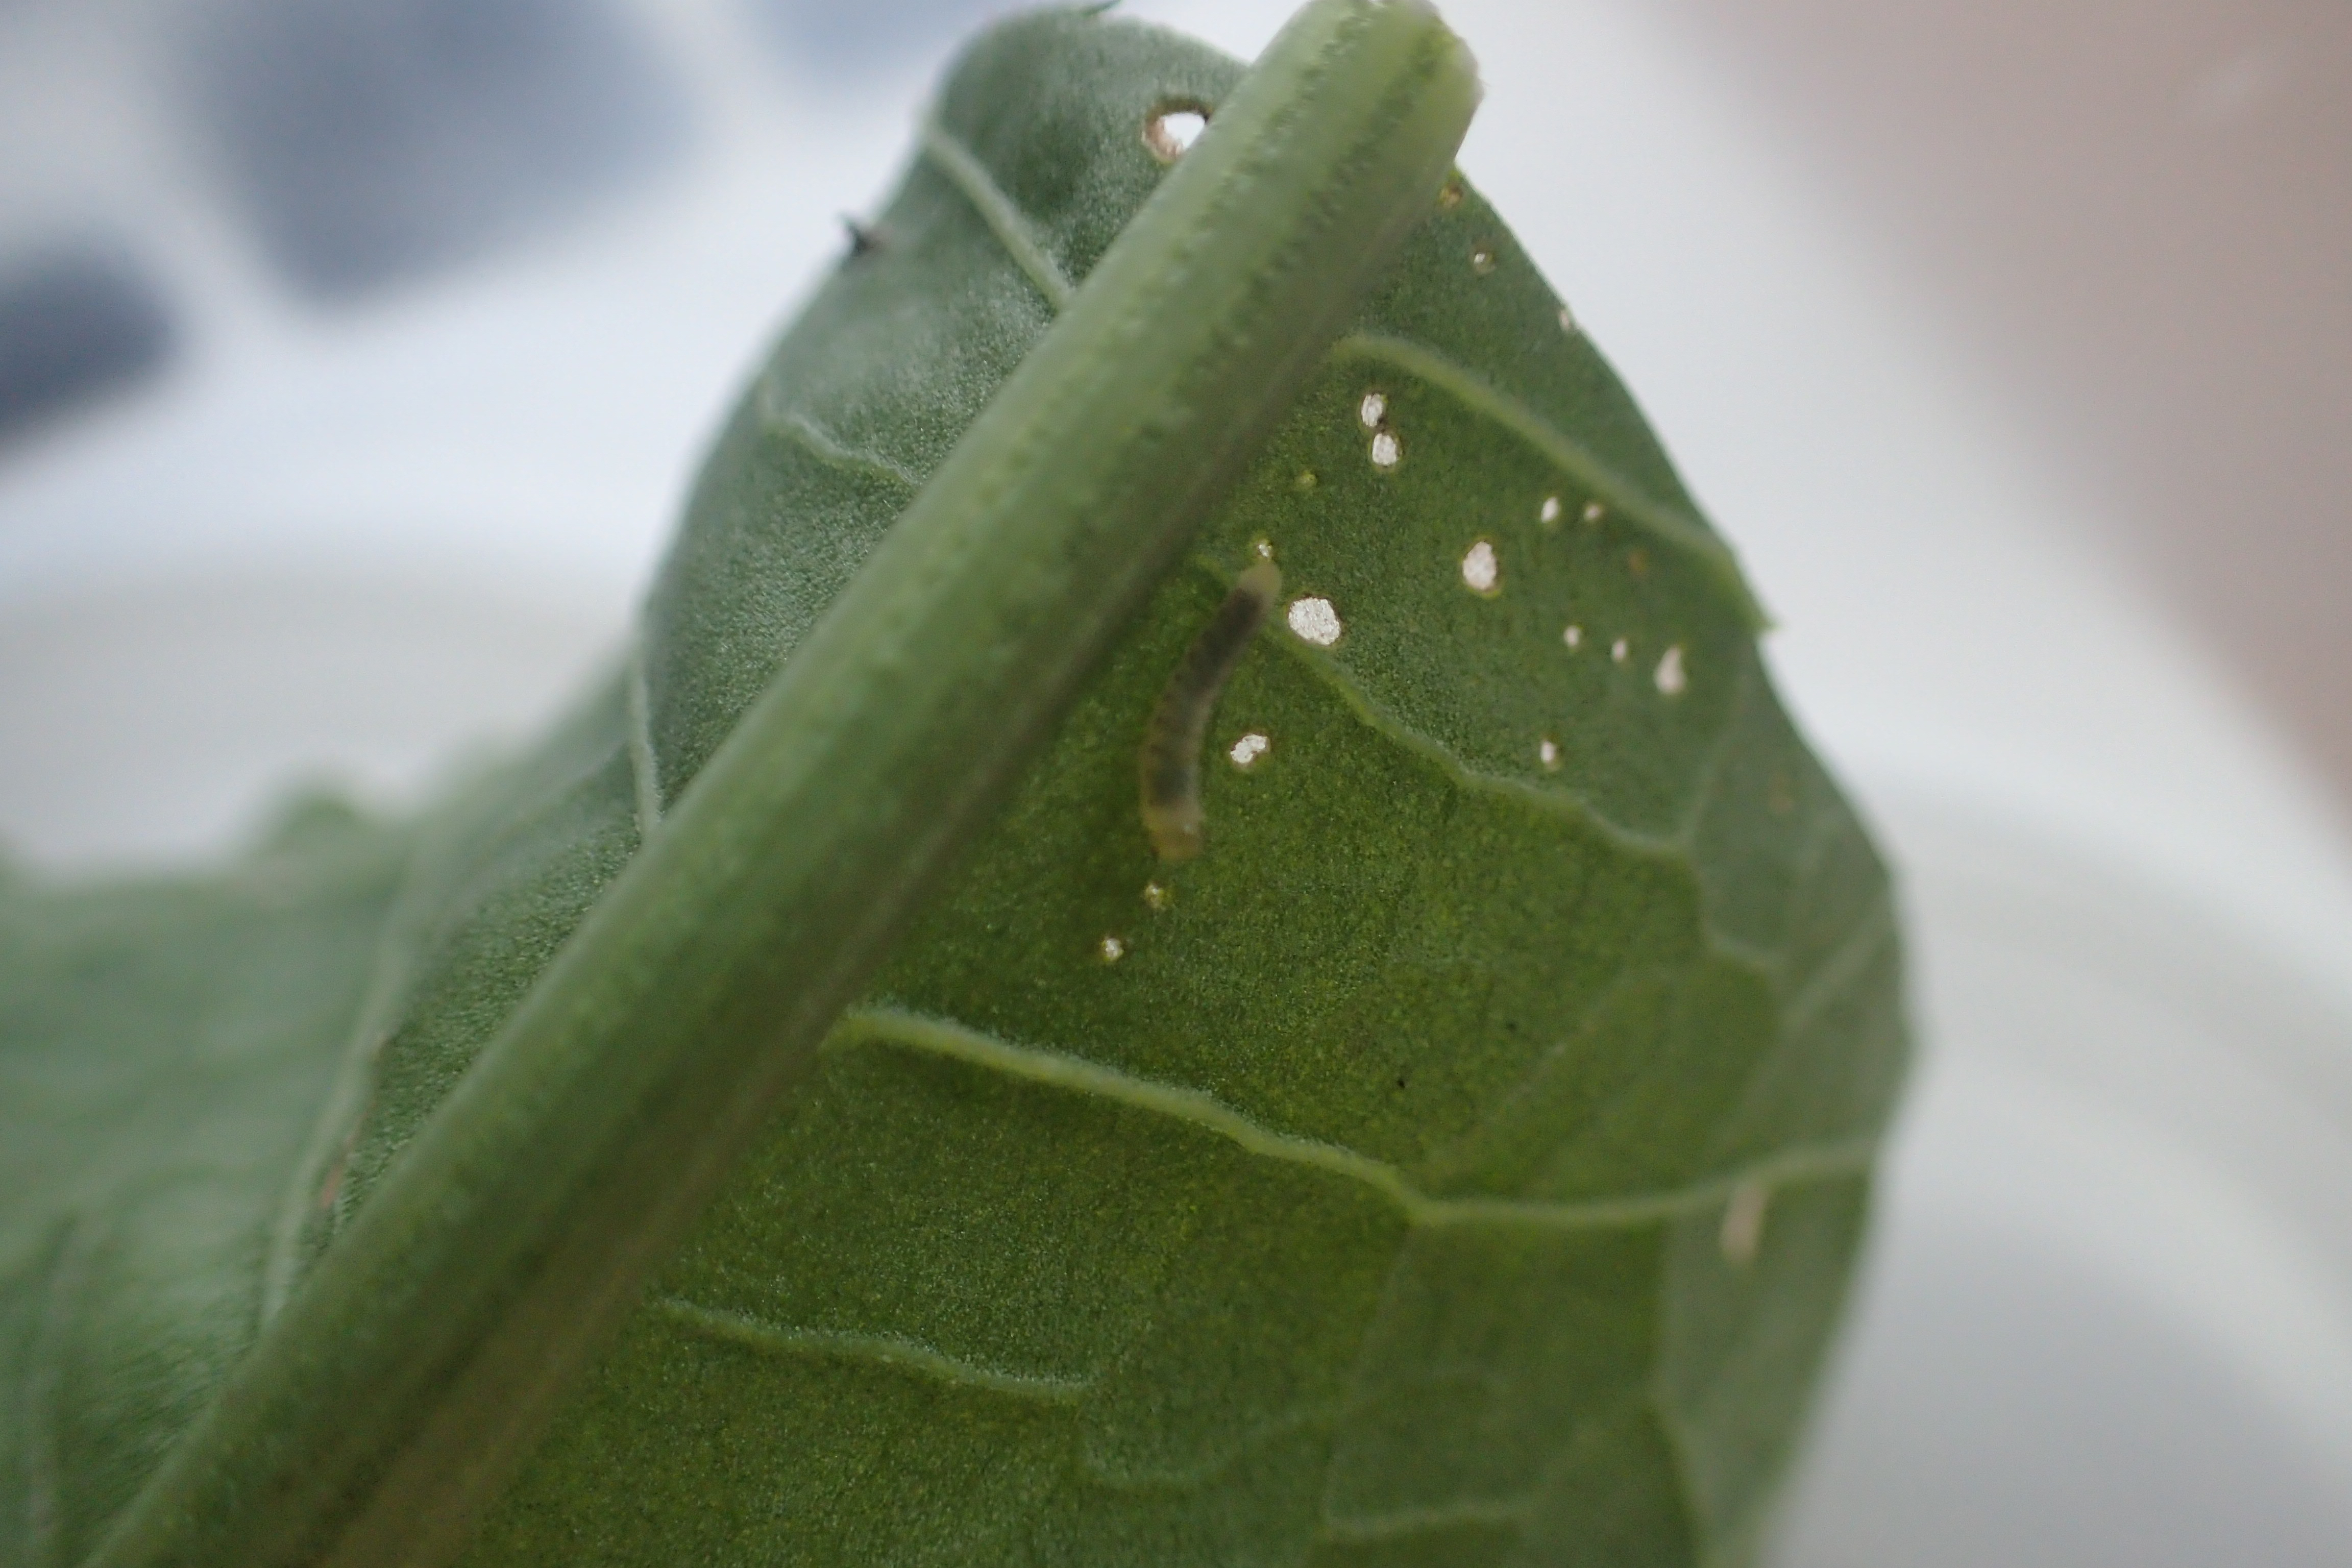
\includegraphics[width=5cm]{photo/hagurohabachi1.JPG}
    \caption{スイバの葉裏でよく見つかったハグロハバチと思われる幼虫}
    \label{pic-hagurohabachi}
  \end{center}
\end{figure}

そのまま, 公園の奥の方にスイバがまばらに生えている方に向かったところ, ほとんど葉がないスイバの, かなり上の方に, ぼてっとした幼虫が写真\ref{pic-sitting-on-branch}のように, とまっているのを発見(以下幼虫1). 
\begin{figure}[htbp]
  \begin{center}
    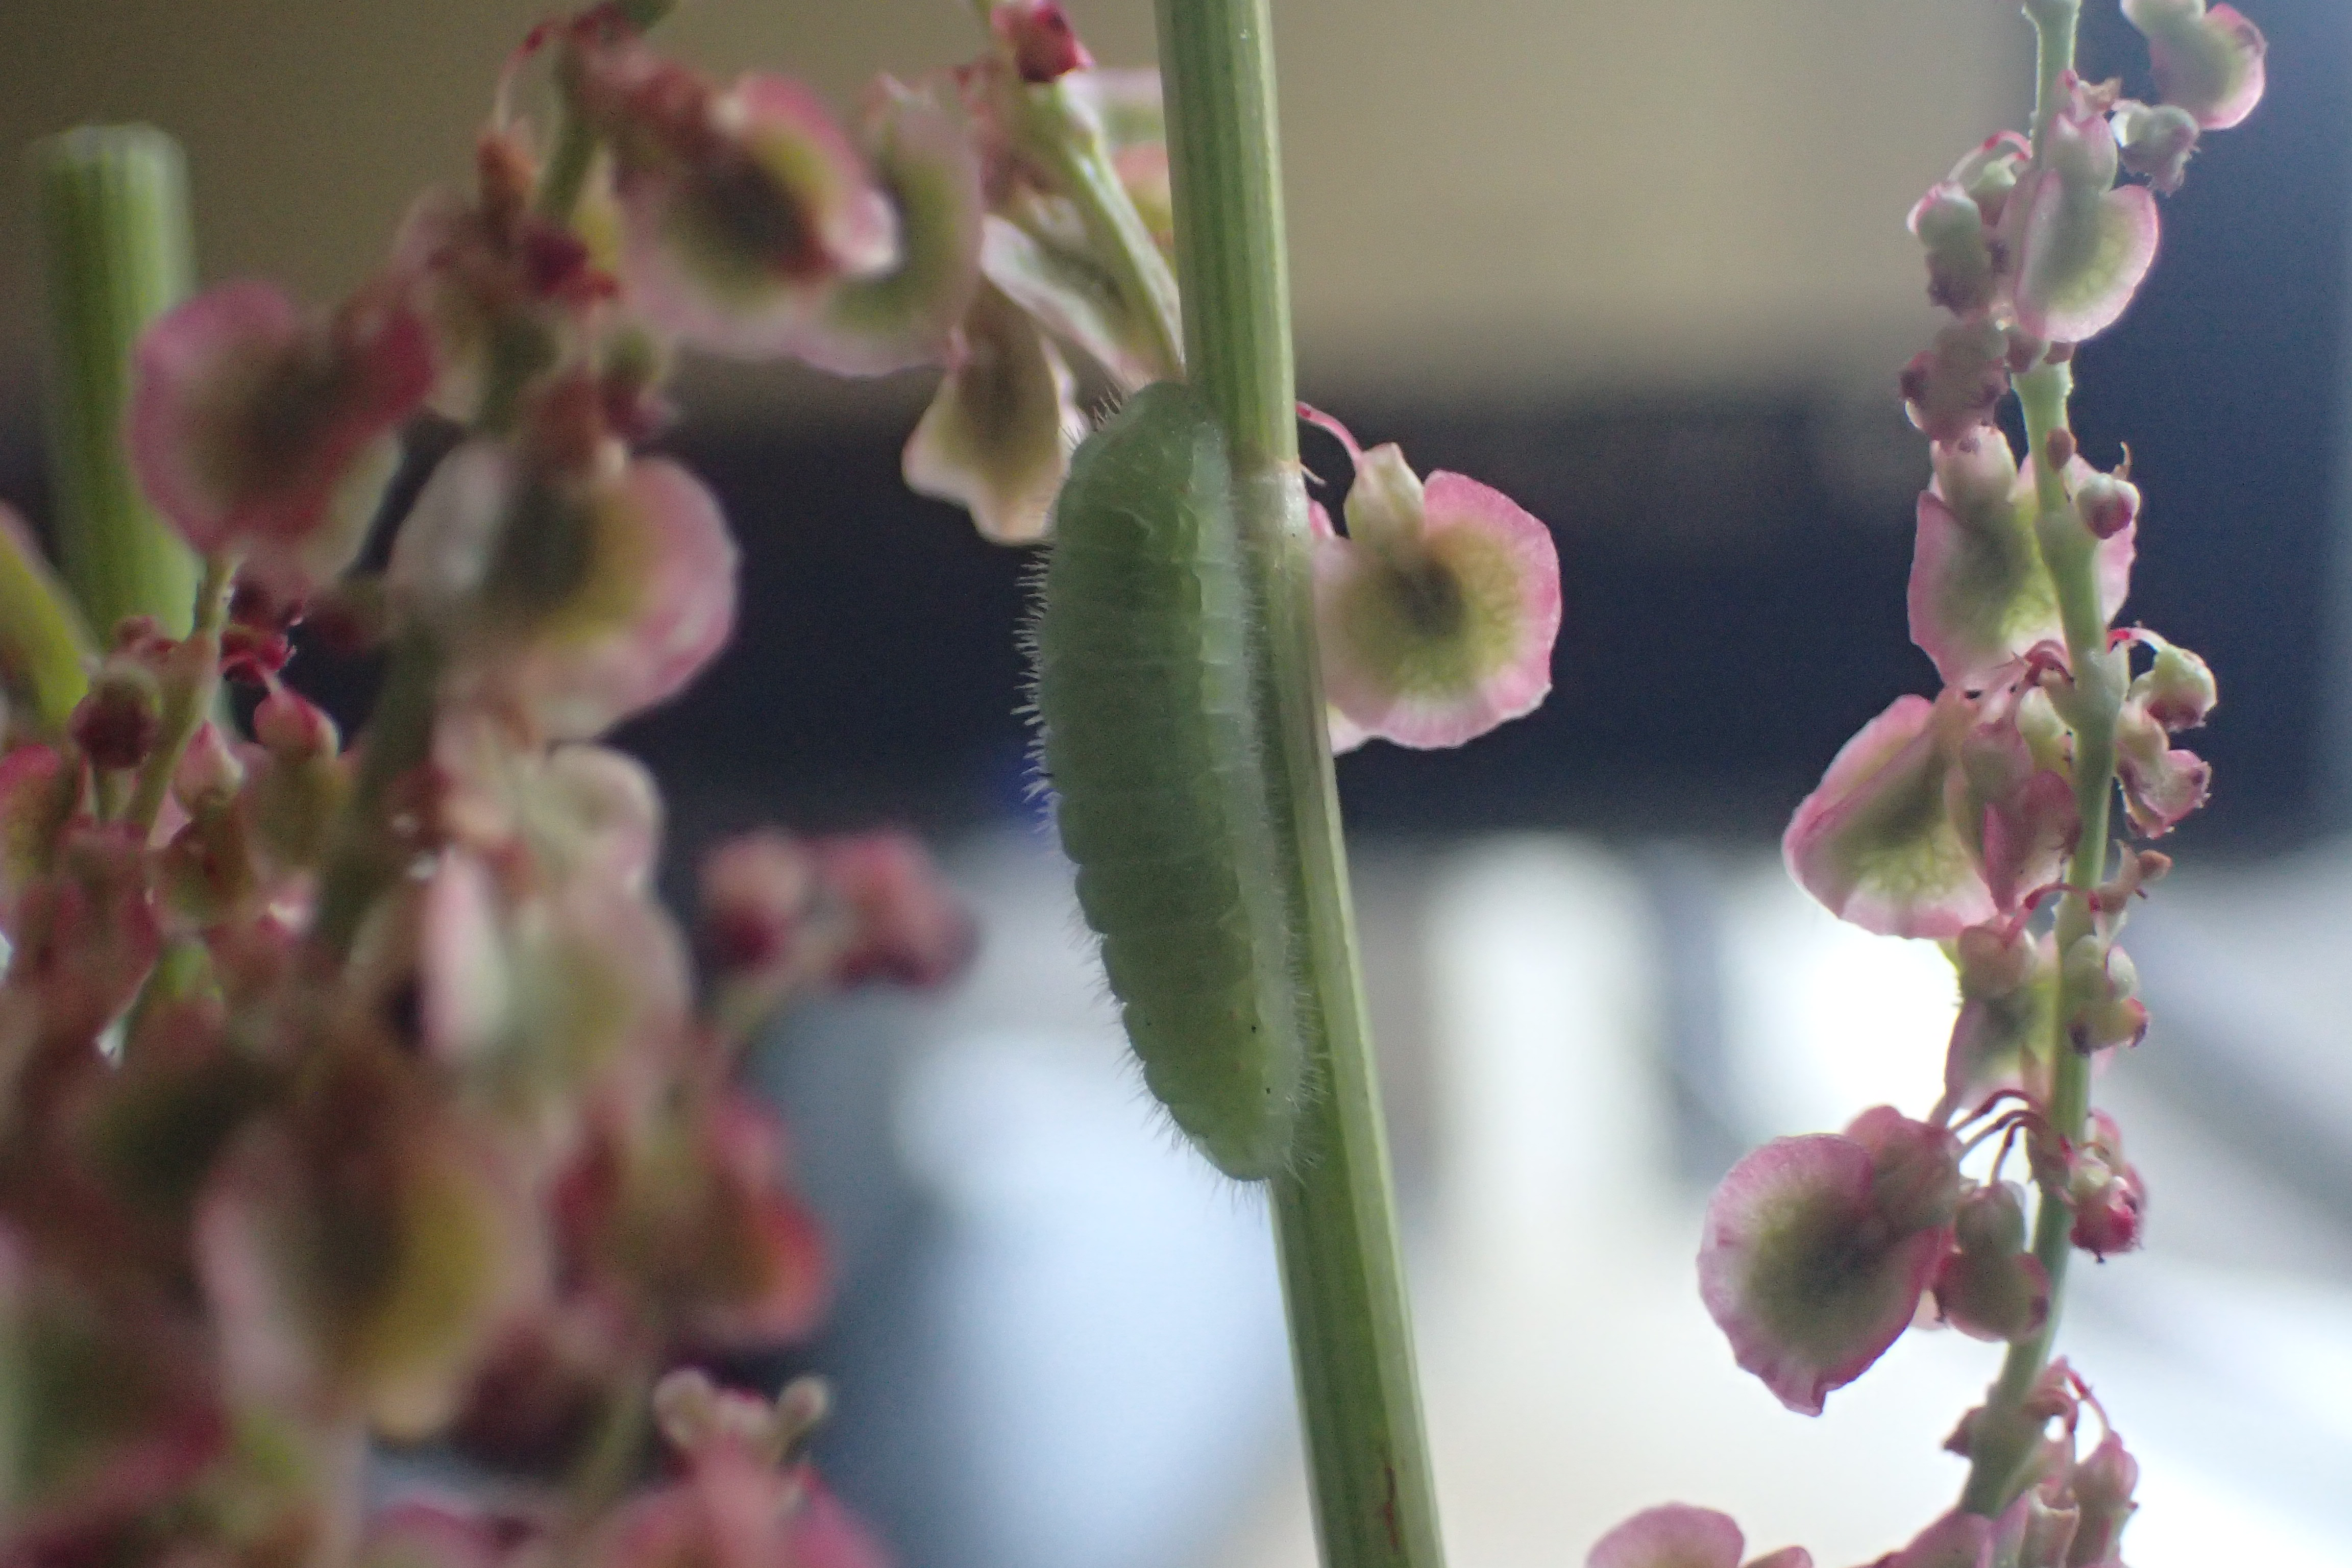
\includegraphics[width=5cm]{photo/sitting_on_branch.JPG}
    \caption{スイバの枝で静止していた幼虫}
    \label{pic-sitting-on-branch}
  \end{center}
\end{figure}

同様なポイントを探したところ, すぐ2匹目(以下幼虫2)が見つかった. 
写真\ref{pic-field}のような, 割とひらけた場所であっさり見つかるようだ. 
\begin{figure}[htbp]
  \begin{center}
    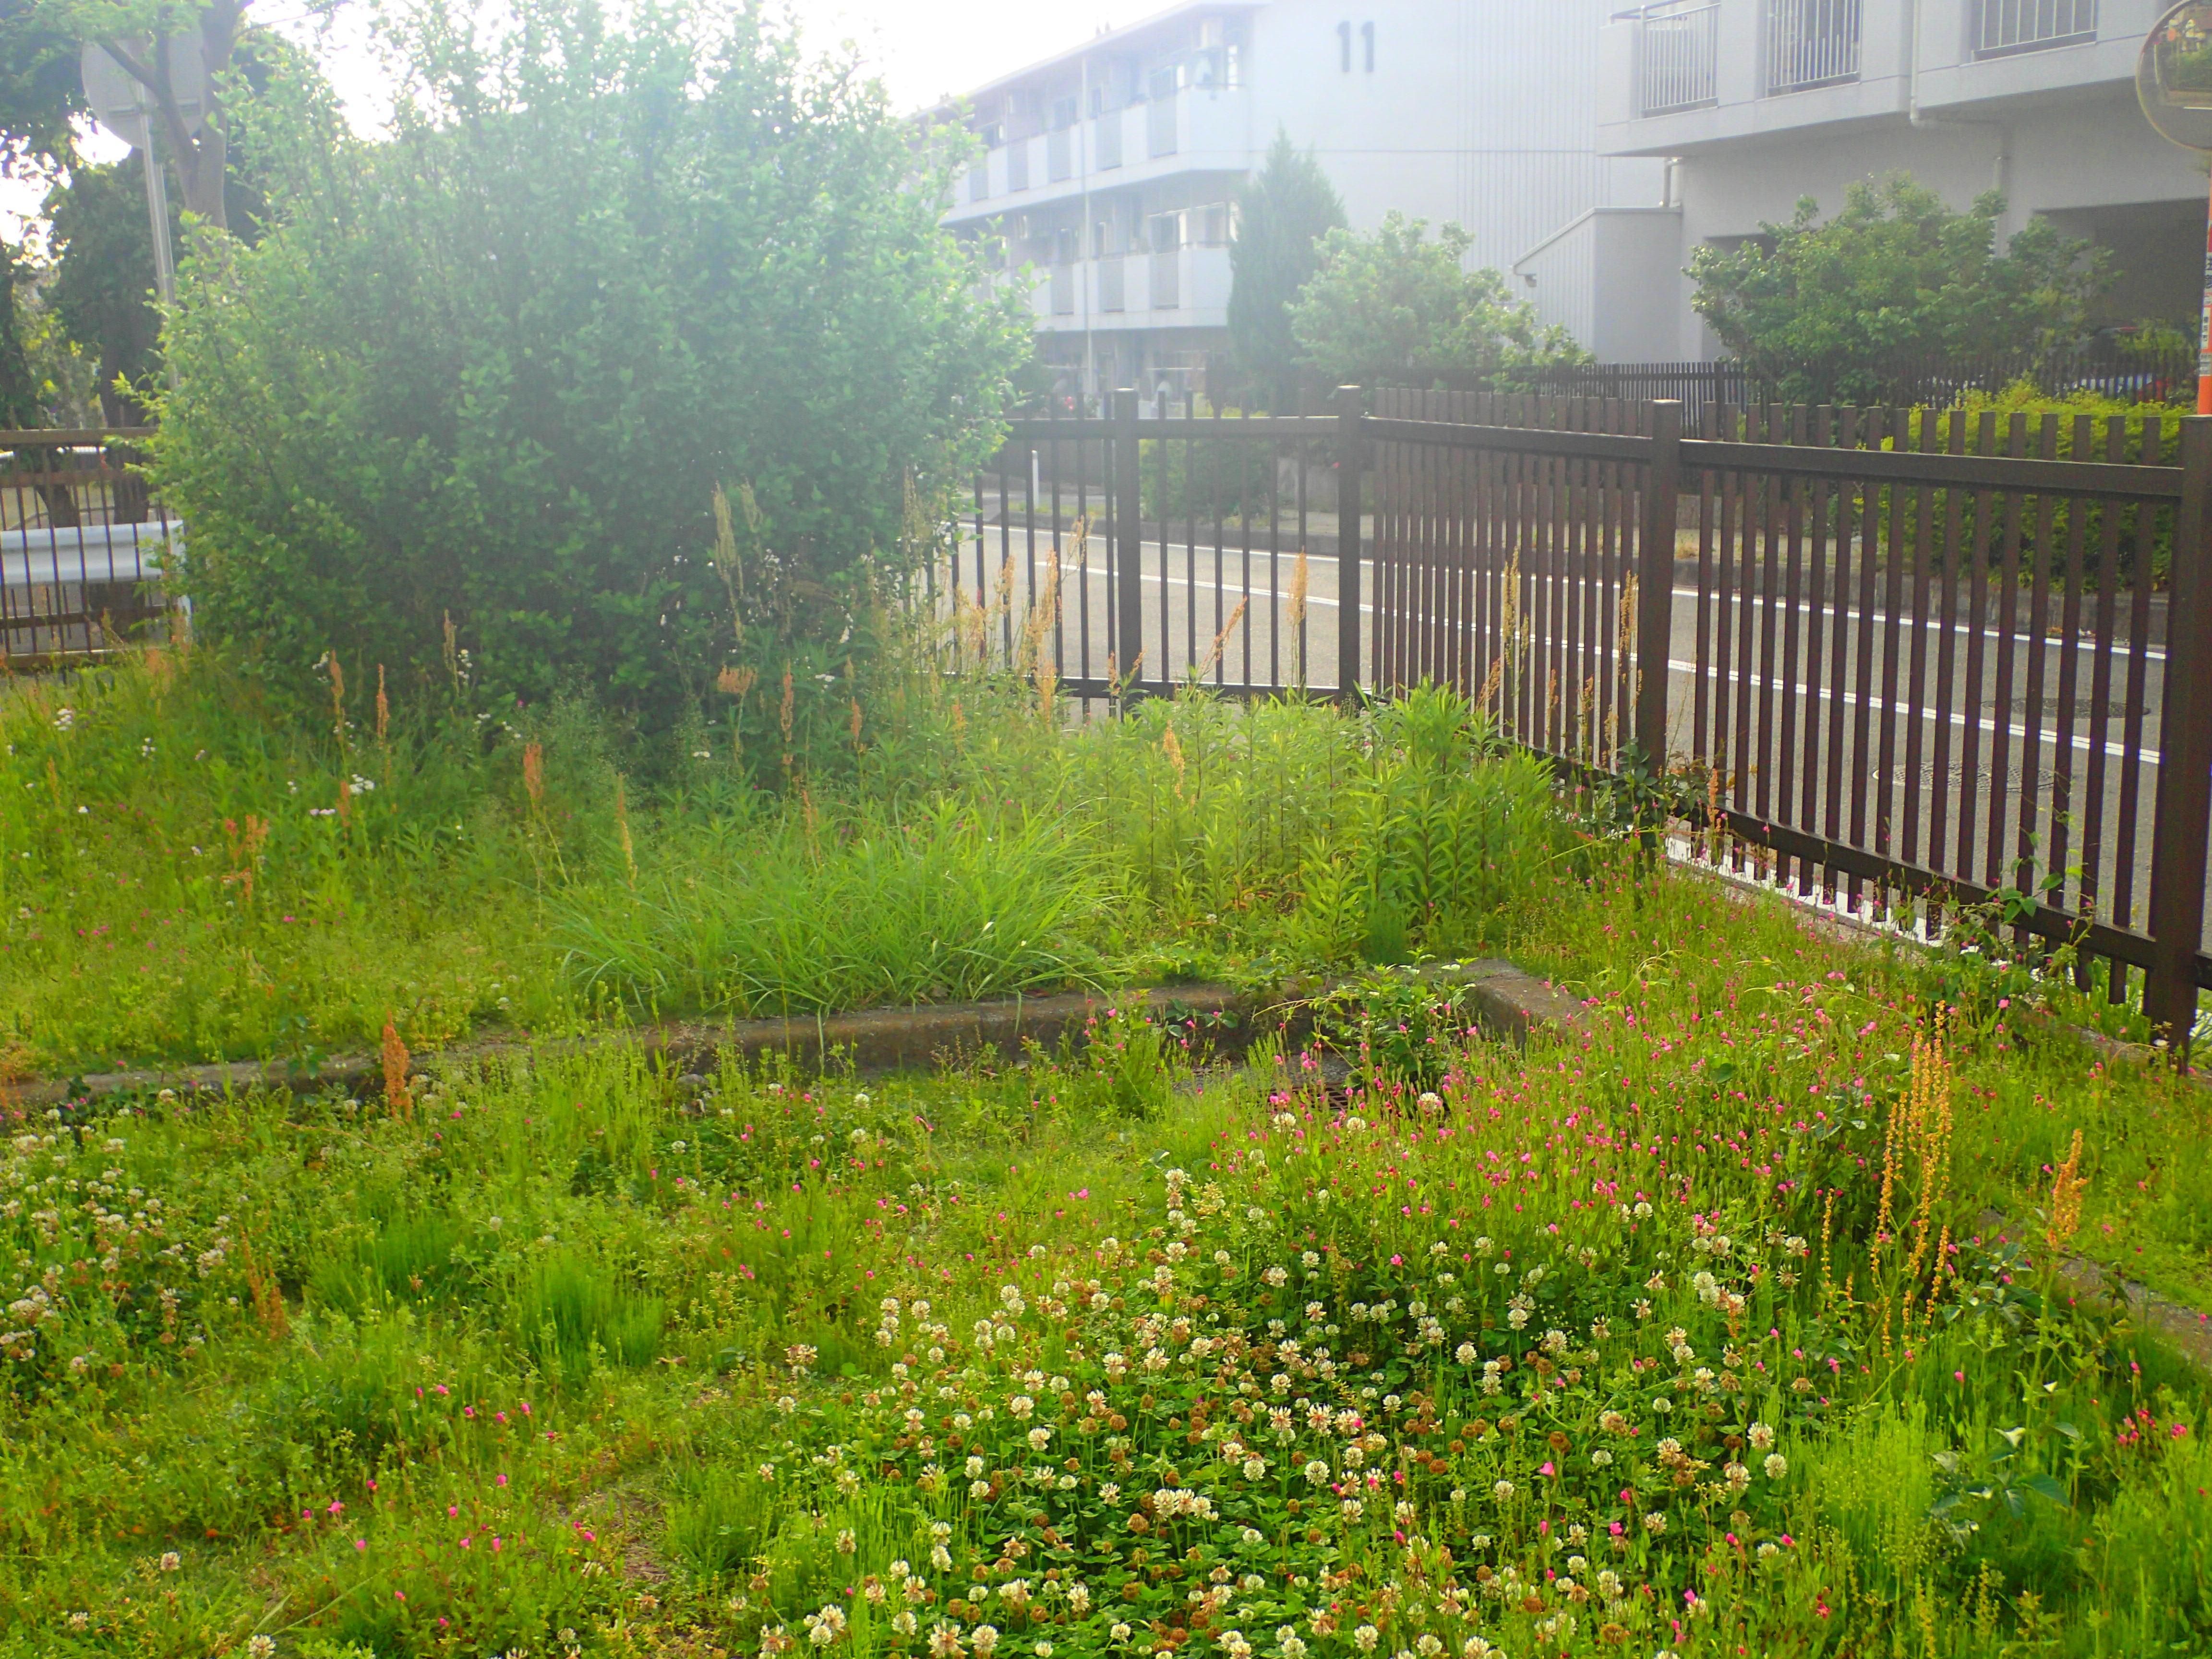
\includegraphics[width=5cm]{photo/park.JPG}
  \end{center}
  \caption{幼虫を発見した公園}
  \label{pic-field}
\end{figure}
幼虫1は, 1cm以上のサイズで, 幼虫2も, 1cm 弱のサイズで, どちらも終齢か, 4齢程度の幼虫と思われる. 
この時期は, 発生サイクル的に, 終齢が多い可能性がある. また, 終齢の幼虫は, 葉裏より, 花を食する可能性がある. 

\subsection{16時半:飼育環境の構築}
まずは, 採集時のスイバが乾燥しないように, 水を満たしたケースにさしたところ, そのわずかな振動で, 幼虫がぽろっと落ちた. 
その後, 幼虫は花によじ登ろうとしているように見えたが, 素直によじ登るというよりも, 頭を振りながら身をよじる動作をしていた. その動作のせいか, 登りかけては落ちるのを繰り返していた. 
脚で食草にしがみつく力は, アゲハ属の幼虫に比べると, 極端に弱いと推測される. 
また, それゆえに, 糸を吐き, 足場を作ろうとして, 妙な動作をしていたのではないかと推測される. 
\begin{figure}[htbp]
  \begin{center}
    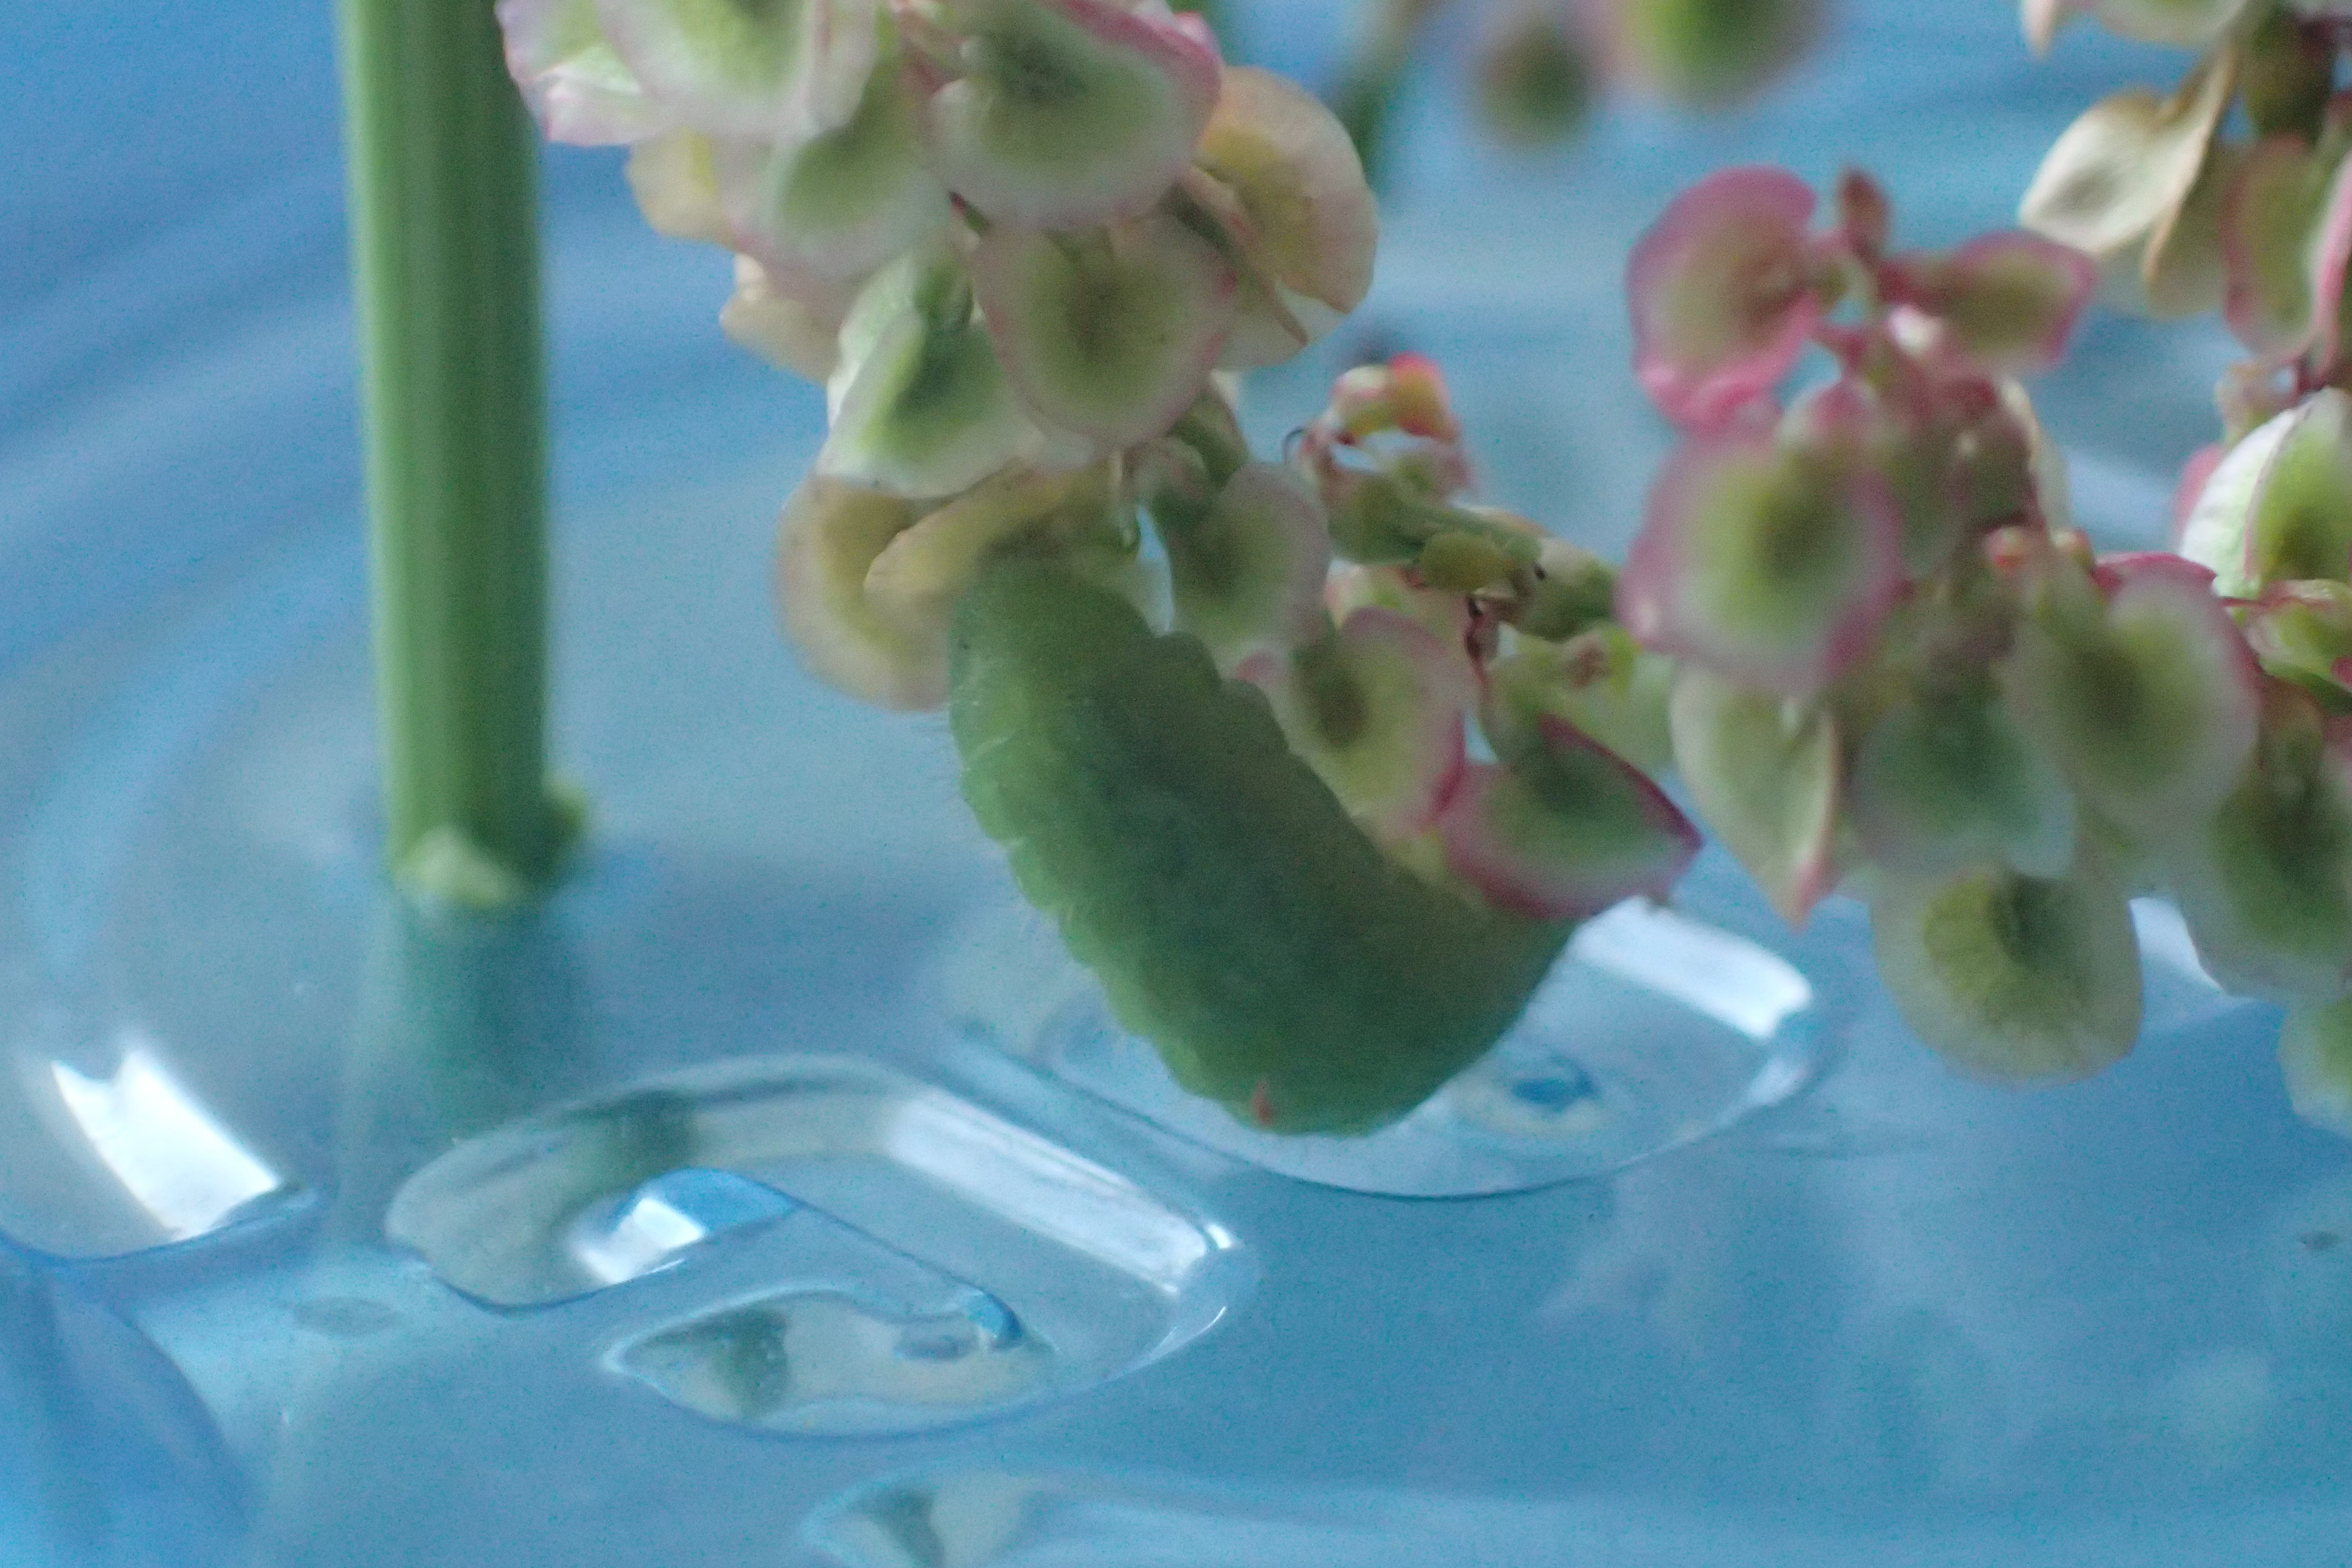
\includegraphics[width=5cm]{photo/try_to_climb.JPG}
    \caption{スイバの花によじ登ろうとする幼虫}
    \label{pic-try-to-climb}
  \end{center}
\end{figure}

\subsection{17時:飼育ケージの変更}
本来であれば, 自然界と同じように, スイバの花が垂直に上に伸びている状況を再現した方がよいと考えたが, 
枝から落下した幼虫があまりにも枝に戻ることができないのと, 世間のベニシジミ飼育のブログなどで, 枝を寝かせた状態で飼育しているものがほとんどであることから, 
枝を寝かせる方向にした. 捨てる予定であった, ガラスの耐熱ボウルを綺麗に洗浄し, スイバの枝に, 湿らせたキッチンペーパーを被せ, 
その上からアルミホイルでくるみ, 写真\ref{pic-environment}のような状況にした. 
\begin{figure}[htbp]
  \begin{center}
    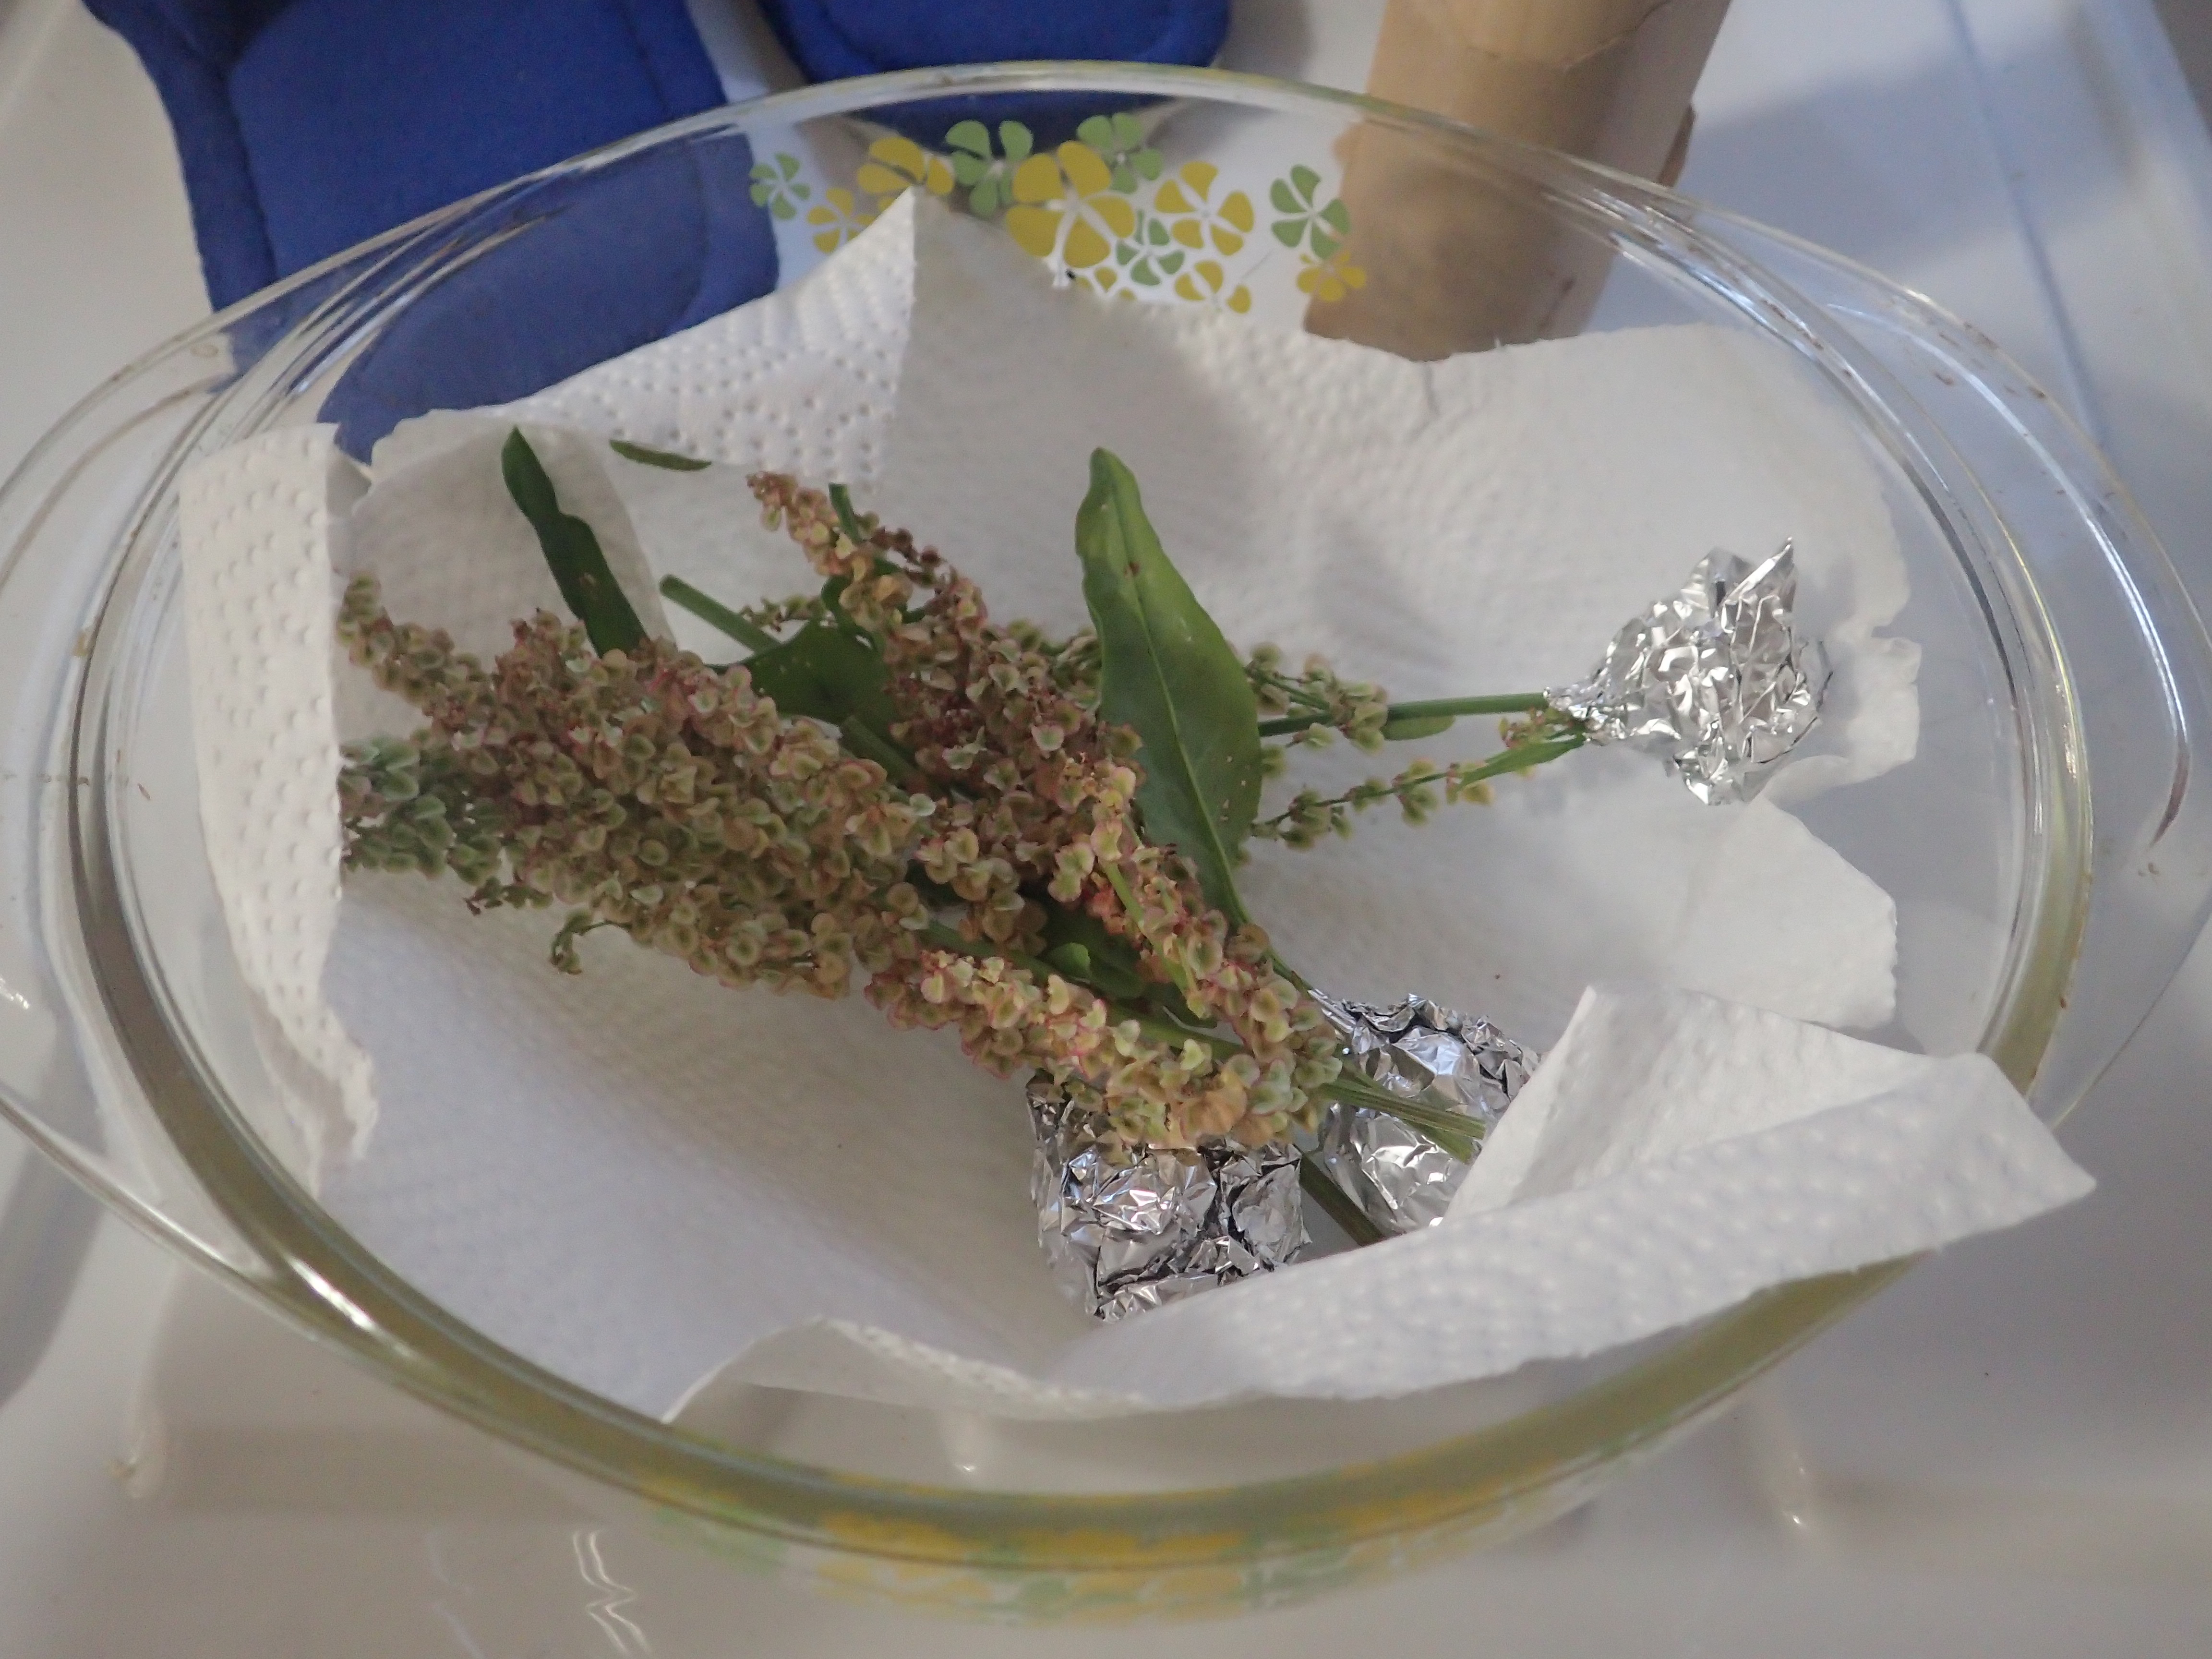
\includegraphics[width=5cm]{photo/environment.JPG}
    \caption{ガラスボウルによる飼育環境}
    \label{pic-environment}
  \end{center}
\end{figure}
また, ガラスボウルの底に, どうしてもスイバから漏れた水がたまり, 幼虫の溺死の危険があるため, 
底にはキッチンペーパーを敷いた. さすがの幼虫も, キッチンペーパーならば足が滑らないのか, 歩きやすそうに動いていた. 
その後, まだ外が少し明るかったので, 太陽光の代わりに, 爬虫類用のUVBランプに日没までの30分程度当てた. 
日本の環境にしては少し紫外線量が多いように思われたが, ガラス越しなので, 半減しているはずで, 問題はないと思われる. 

\subsection{18時:幼虫の移動}
食草の上を移動していた幼虫が, 2匹ともキッチンペーパーに降り, 移動を始めた. 
どこに移動するか見ていると, 写真\ref{pic-environment}の左上(よく見ると紙の裏から体がはみ出している)ように, やたらと紙の裏, 折れ曲がったところなどに移動して, そこで静止する様子が見られた. 
おそらく, 休む時は, 葉などの裏に隠れる習性からの行動であろうと思われる. 

\subsection{20時:活動の再開}
キッチンペーパーの裏でそのまま静止して翌朝まで寝てしまうのかと思ったが, 1時間程度しか静止しておらず, また移動し, 食草を食べている様子が確認できた. 
おそらく, 夜間でも, 短時間の休息と移動を繰り返すことで, 天敵に見つかる可能性を下げているのであろうと思われる. 
人間や, 犬猫と違い, 夜間にずっと寝ている, ということは無いようだ. 

\subsection{23時:糞の観察}
糞は, やや明るめの焦げ茶色で, 1mm程度の樽型のものが10個ほど確認できた. 

\newpage
\section{5/12の記録}
\subsection{9時:特に異常なし}
思いの外大量の糞をしていたので, 古い食草を捨てるとともに, 掃除. 
昨日, 枝に登るのに苦労していた個体も, しっかり枝に捕まって静止していた. 
寸法を測定したところ, どちらも15mm*5mm程度で, 思ったより寸法差はなかった. 
葉が食われていたが, 表面だけを舐めるような食痕ではなく, 写真\ref{Larba-day2-2}のように, アゲハのような食痕であった. 
他のブログなどと矛盾するが, 与えている葉が, 柔らかい若い葉であることが要因なのかもしれない. 

\begin{figure}[htbp]
  \begin{minipage}{0.5\hsize}
    \begin{center}
      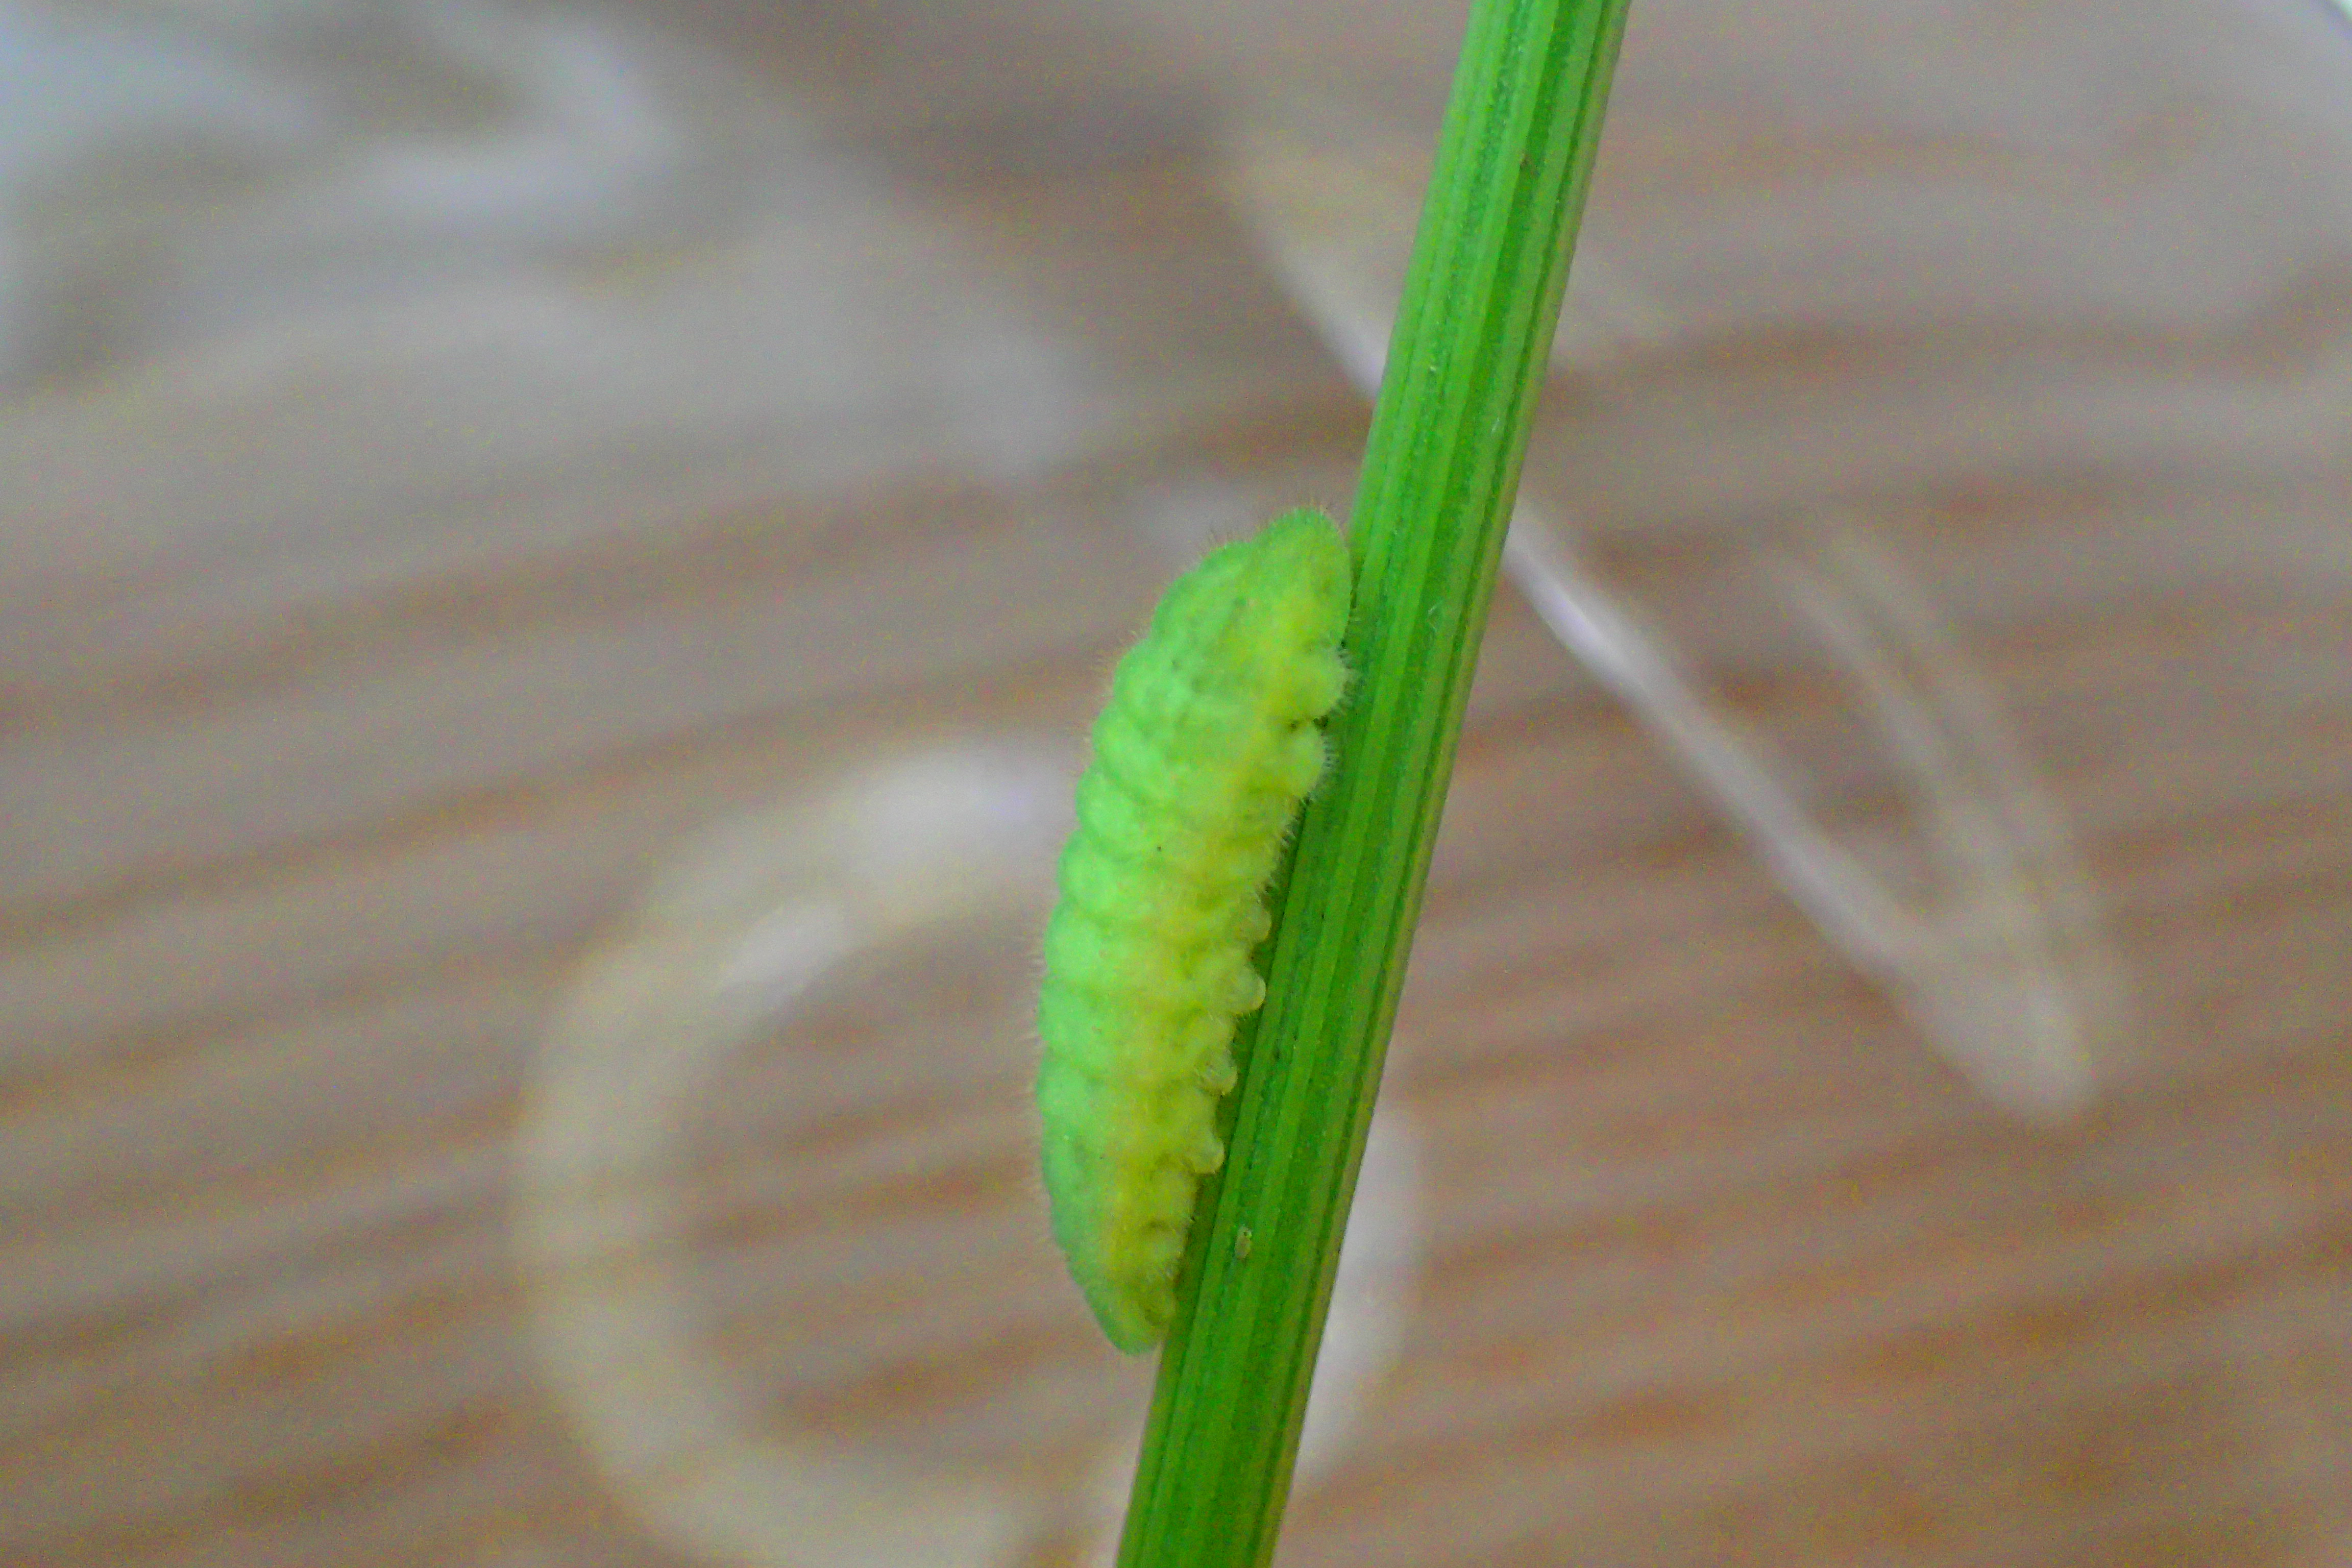
\includegraphics[width=5cm]{photo2/Larva1.JPG}
    \end{center}
    \caption{幼虫1の状態}
    \label{Larba-day2-1}
  \end{minipage}
  \begin{minipage}{0.5\hsize}
    \begin{center}
      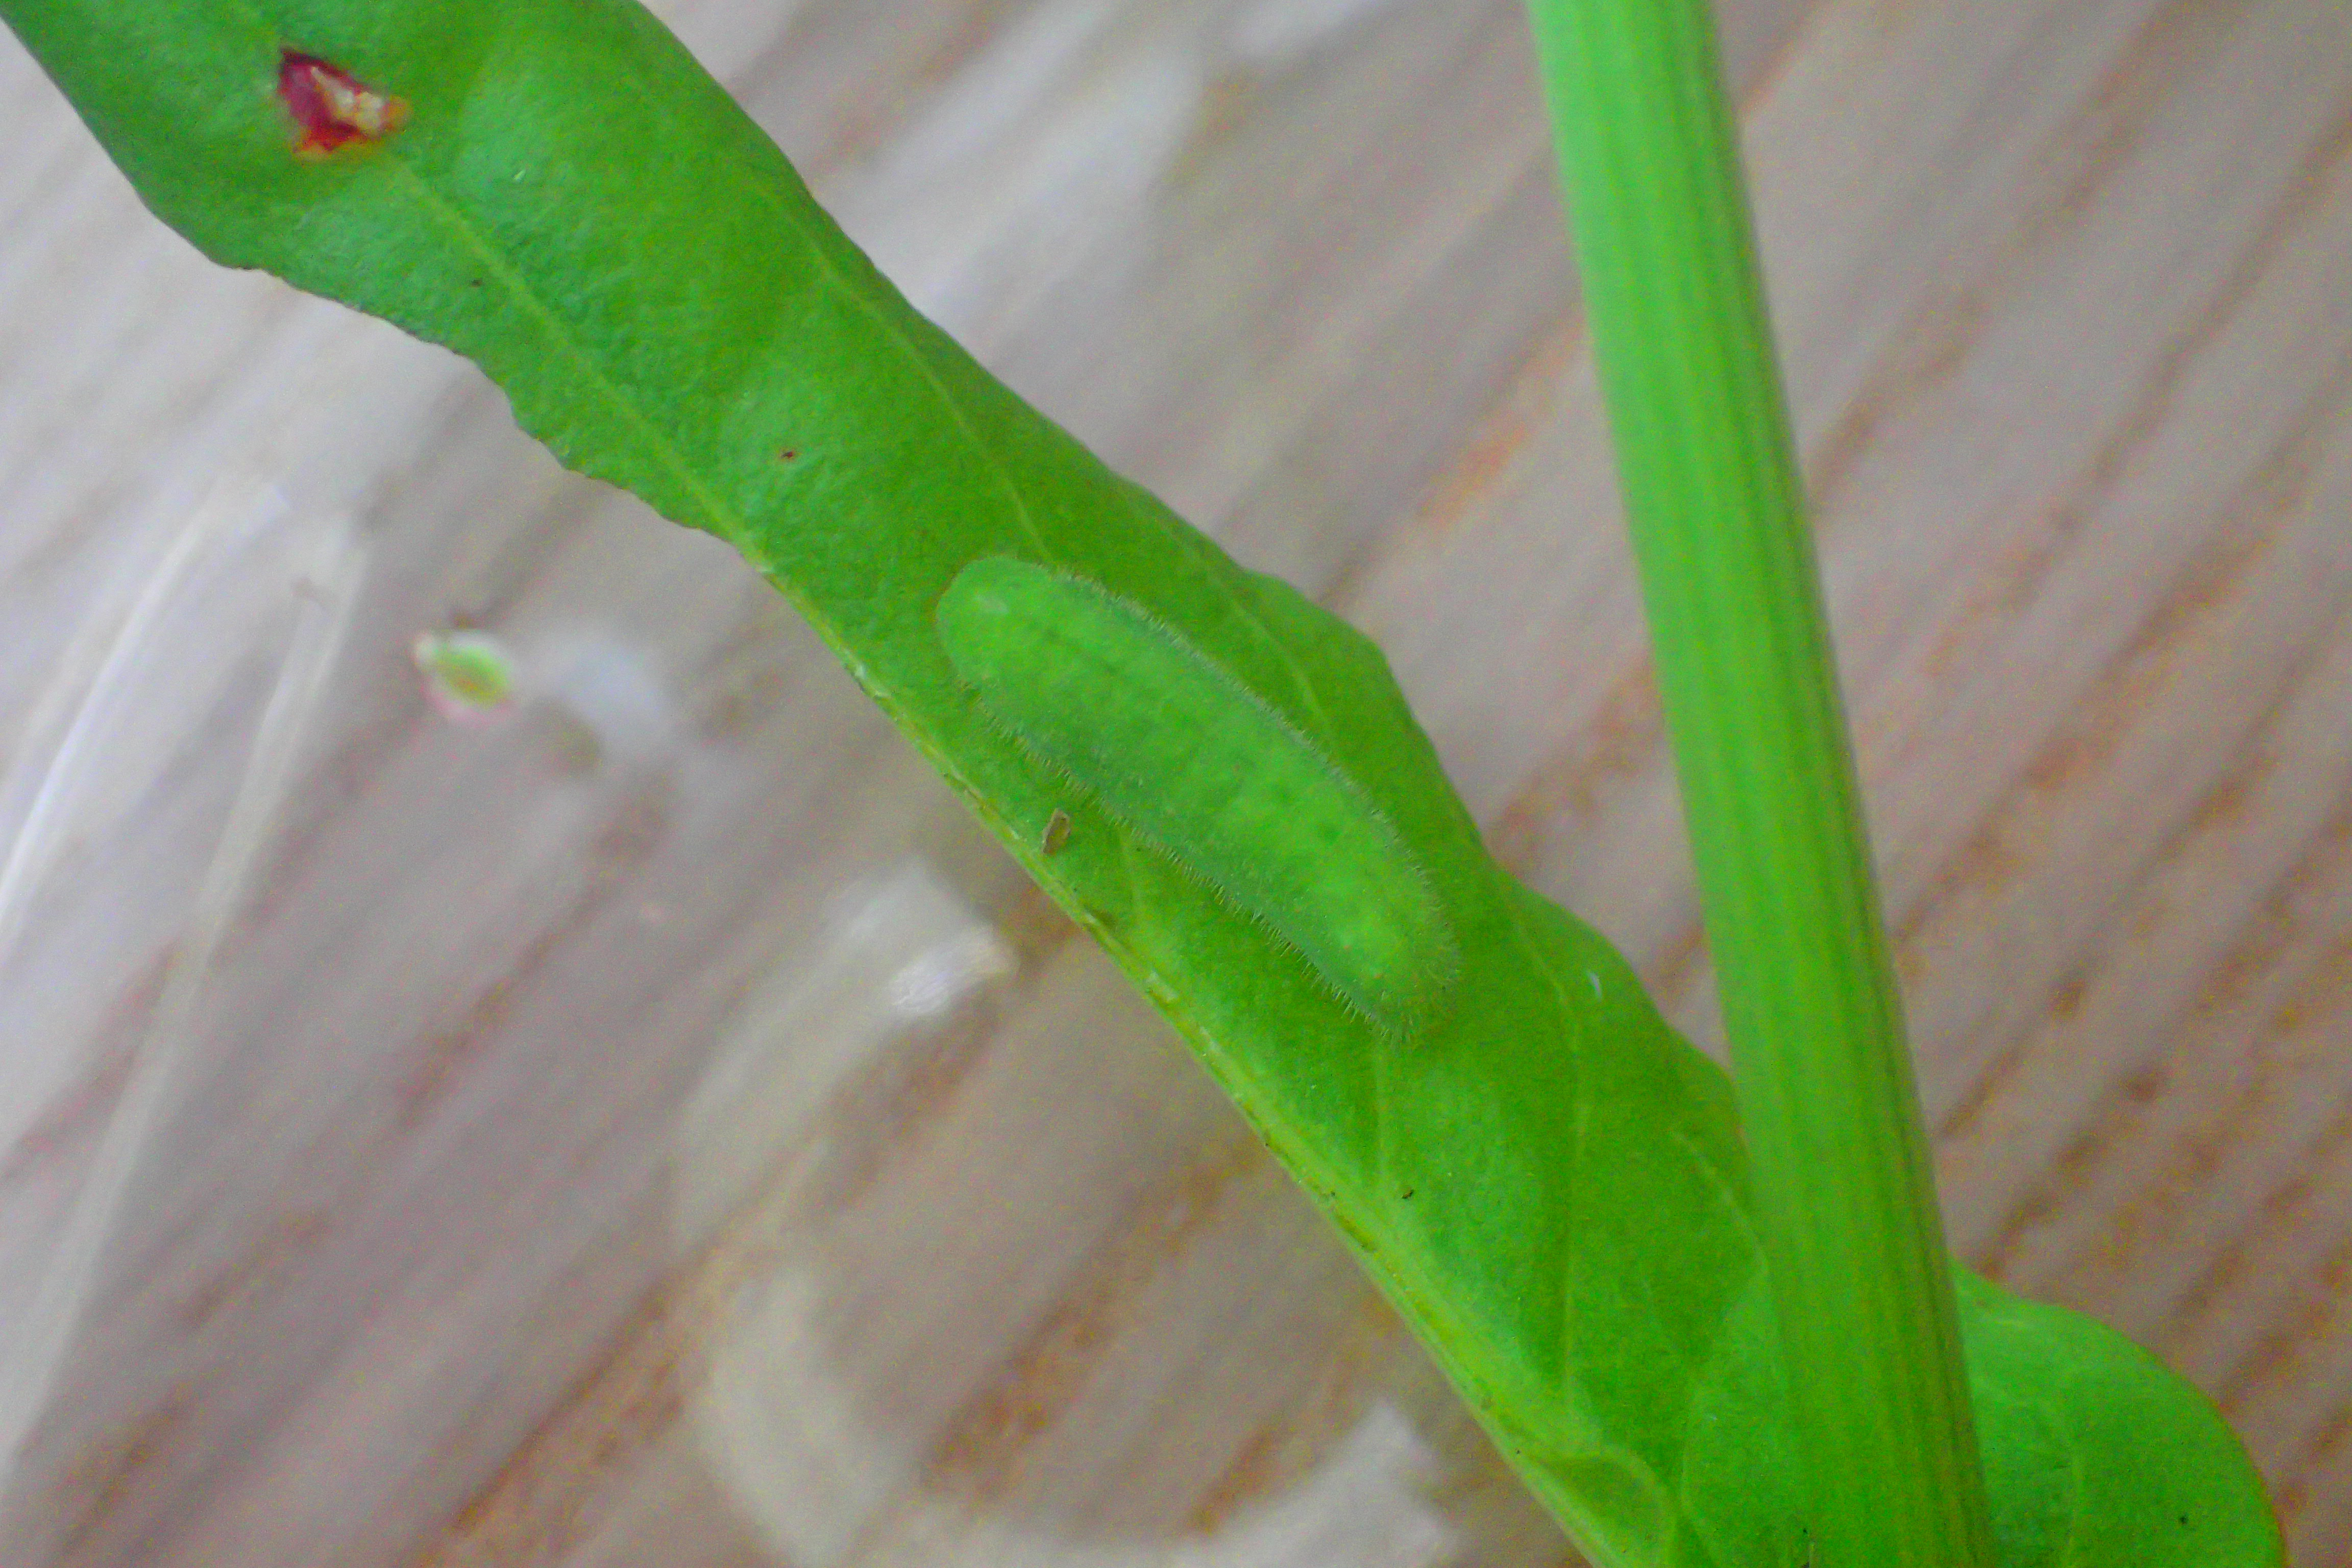
\includegraphics[width=5cm]{photo2/Larva2.JPG}
    \end{center}
    \caption{幼虫2の状態}
    \label{Larba-day2-2}
  \end{minipage}
\end{figure}

\subsection{15時:餌の採取と幼虫の居場所}
幼虫の採集場所と同じところに, 新しい餌用のスイバを取りに行ったついでに, 
幼虫を探した. 簡単に, 同じ苗で2匹見つかったが, やはりどちらも, 花に近いところの枝, 花の中で見つかった. 
やはり, 幼虫はあまり葉にいないのだろうか. 
家に帰り, ケージ内の幼虫がどこにいるか見たところ, 2匹とも花を避け, 葉の上にべったりとくっついていた. 
単純に花, 葉というより, 鉛直方向に上を目指す傾向があるだけなのか. 
よくわからない. 

\subsection{16時:鶴見川堤防のギシギシで幼虫を探す}
会社に行く用事を済ませたのち, 鶴見川沿いの堤防に群生するギシギシに幼虫がいないか探してみた. 
鶴見川の堤防は, 写真\ref{pic-Tsurumi-River}のような, ギシギシの群生があちこちに見られ, ベニシジミの食草は豊富である. 
\begin{figure}[htbp]
  \begin{center}
    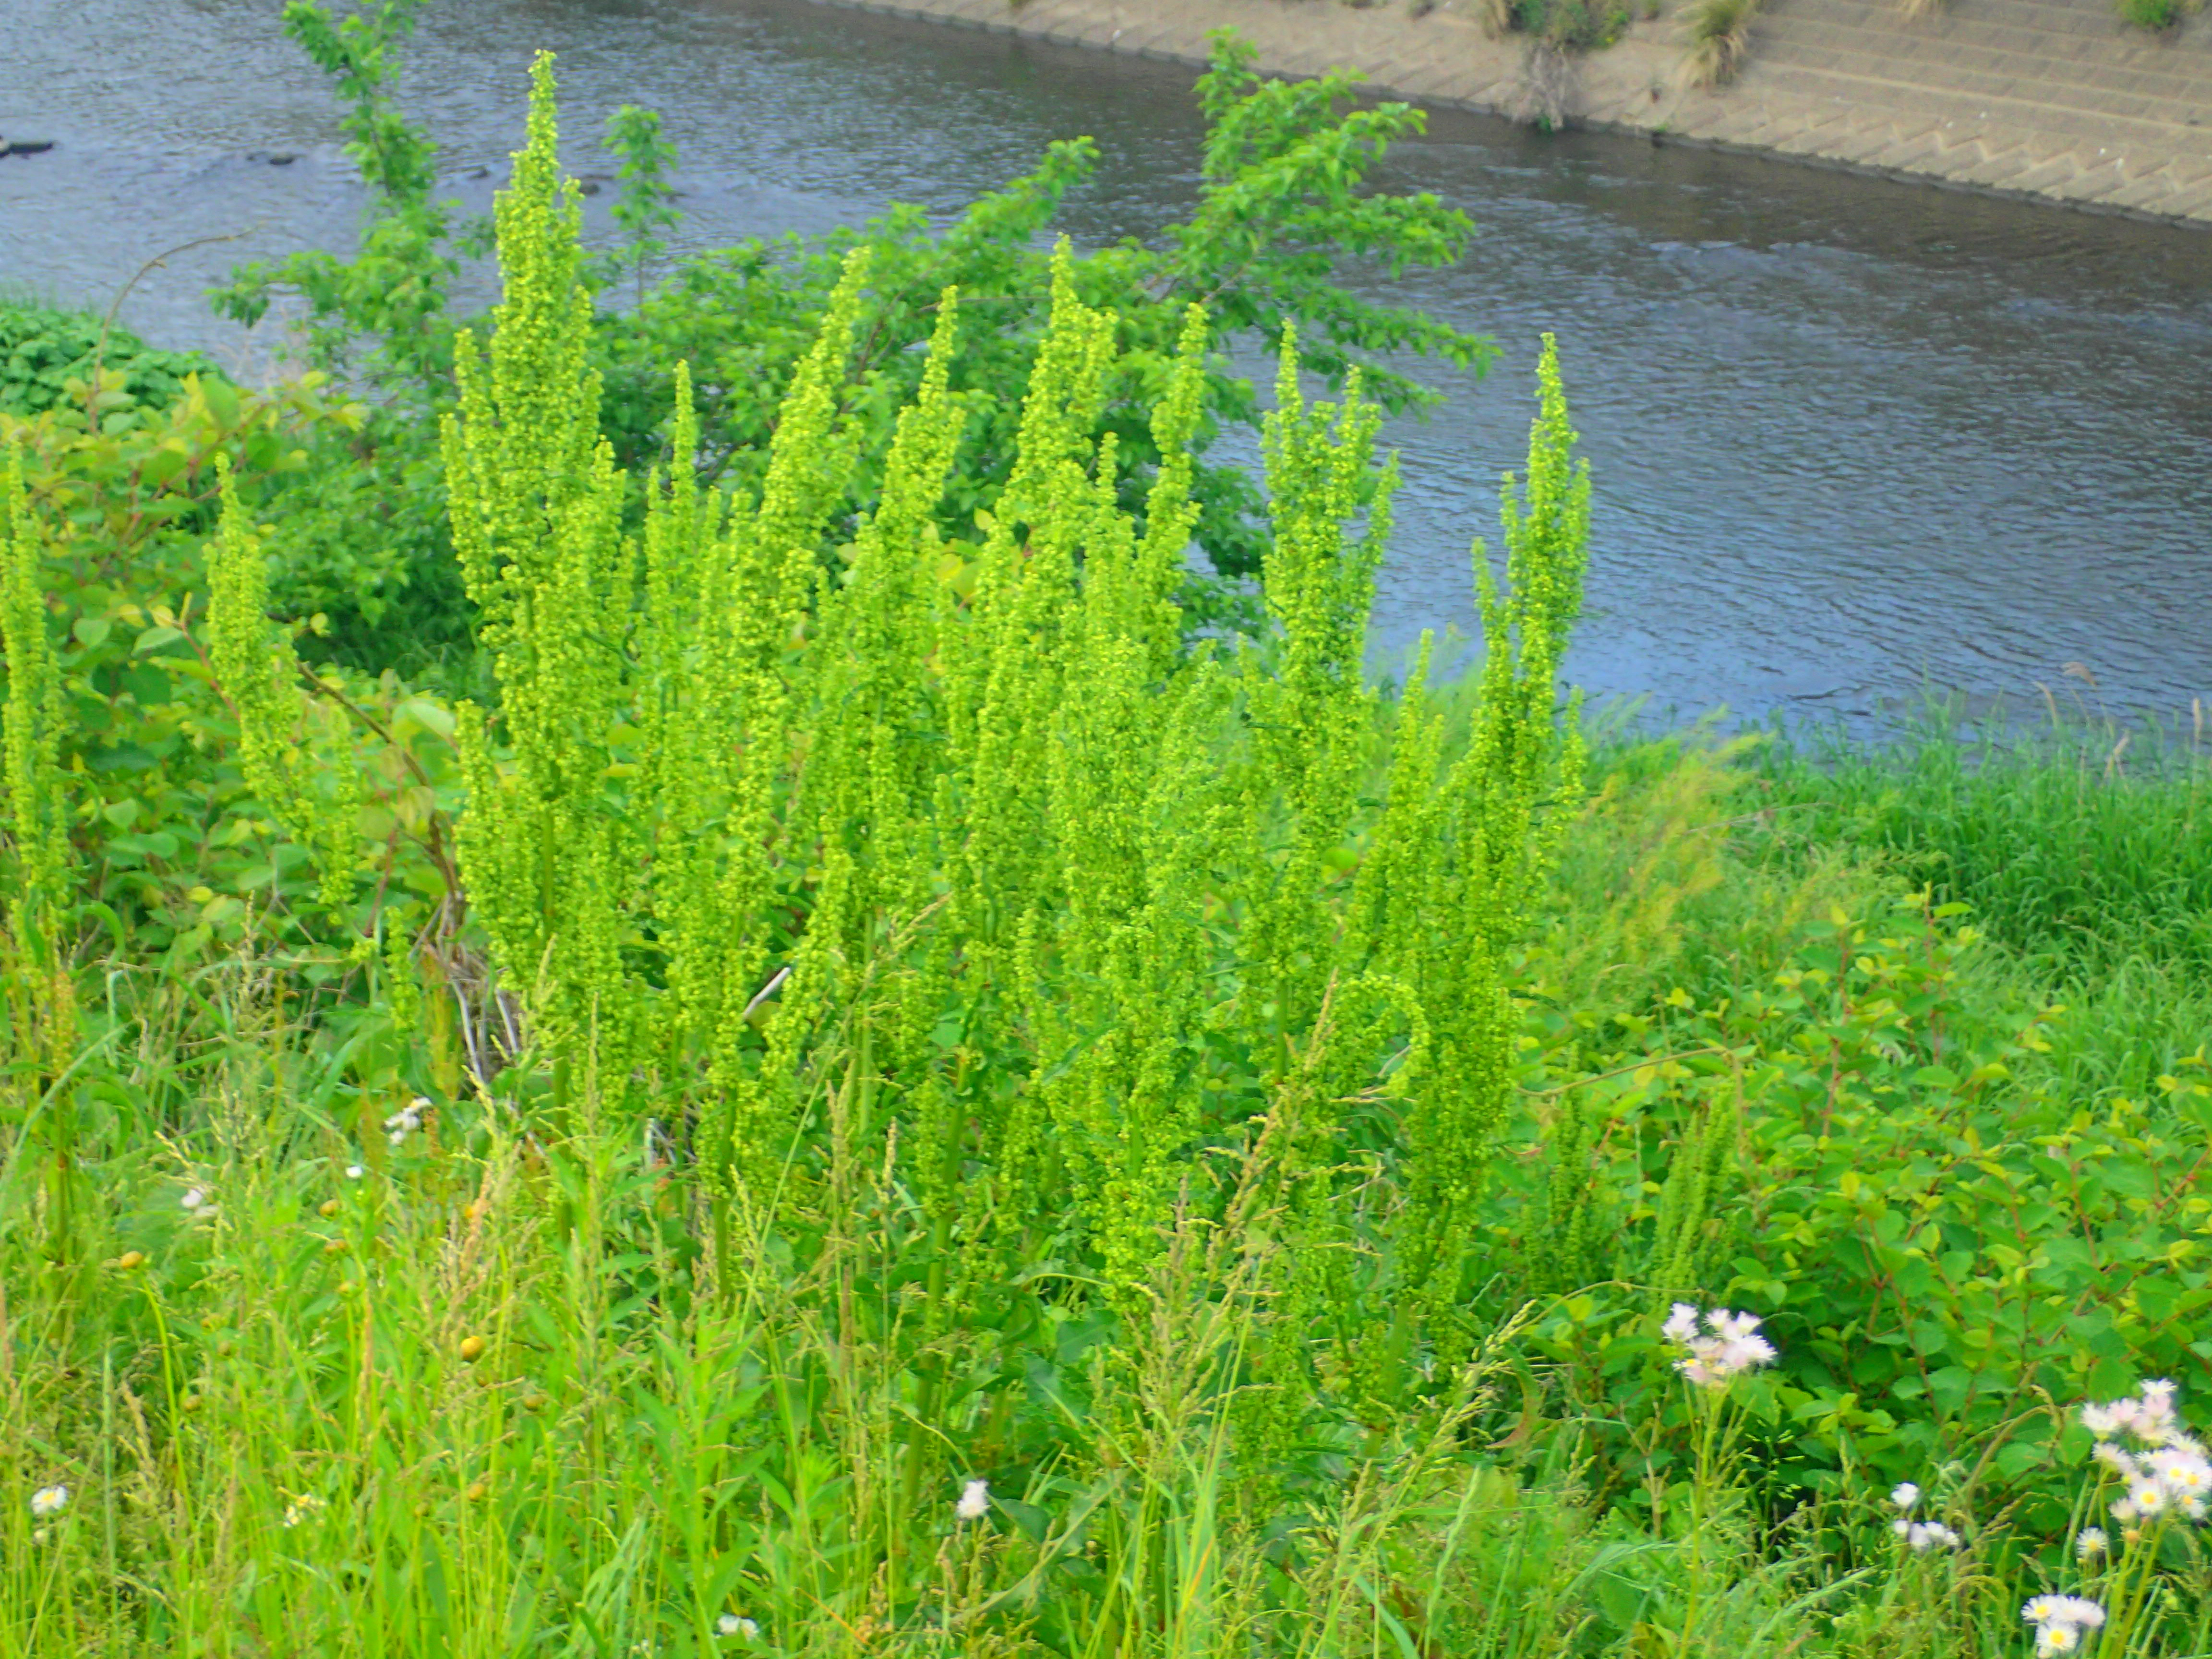
\includegraphics[width=5cm]{photo2/TsurumiRiver.JPG}
  \end{center}
  \caption{ギシギシの群生}
  \label{pic-Tsurumi-River}
\end{figure}
また, 定期的な草刈りこそはいるものの, 自然環境としては良好で, 様々な植物が生えている. 
ところが, 公園ではあっさり見つかった幼虫が, どれだけ探しても見つからなかった. 
ハグロハバチの幼虫ですら, 見つかりはしたが, 公園と比べると極端に数が少なかった. 
理由はわからないが, 状況証拠として, 
\begin{itemize}
  \item 鶴見川の堤防は, スイバも存在するが, ギシギシが極端に多い
  \item 鶴見川の堤防は, ギシギシ, スイバ以外に, 背の高い植物が多い
  \item 鶴見川の堤防は, いつも割と強い風が吹いている
\end{itemize}
というような環境要因があり, どうもベニシジミは, ギシギシよりはスイバを好み, 割とひらけていて草がまばらな, 風のそれほど強くない環境を好むのかもしれない. 
特に, 風については, ベニシジミ幼虫の, しがみつく力の弱さからすると嫌がりそうな気がする. 
また, ギシギシの葉は, スイバの葉よりも明らかに固そうで, 幼虫が食す上では, あまり好まれそうにない. 

\subsection{19時:特に異常なし}
糞の掃除, 餌の交換を実施. 相変わらず幼虫は葉の上にいる. 自然界と何が違うのか. 彼らが花に向かわない理由が, 
今の所, 苗が鉛直に立っているか否かしか想像できない. 
ついでに, 鶴見川堤防沿いの, ギシギシの葉も餌として追加してみた. 結局どちらの葉におちつくか楽しみだ. 

\section{5/13の記録}
\subsection{9時:特に異常なし}
餌を見たところ, ギシギシには全く食いついていなかった. 
やはりスイバの方が好きなよう.

\subsection{13時:幼虫にダメージを与えてしまったか}
朝から, 日光に当てる目的で, 外にケースを出していたが, 
ガラスボウルの特性により, 中に熱気がこもり, サウナ状態になっていた. 
スイバはしおれ, 幼虫も何やら元気がない. 

\subsection{19時:幼虫のダメージは深刻かもしれない}
幼虫が, 動いてはいるものの, やたら体を丸めたり捻ったりして, 体勢がおかしいのと, 餌をあまり食っていない. 
ふんが, 下痢のようになっている. 葉に戻しても, すぐ丸まってひっくり返る. ちょっとまずい. 

\subsection{23時:とりあえず体勢はおちついている}
体勢は水平なまま落ち着いているが, 餌をくったり糞をした形跡がない. 体液なのか, 下痢なのかわからないが, 
赤茶色いシミがあちこちにある. とりあえず明日から外に出すのはやめる. 

\section{5/14の記録}
\subsection{9時:もう死んでいるかも}
まったく動かず, 餌も食べていない. 糞の排出もない. 赤茶色の汁も少し出ている. 
もうダメかもしれない. 高熱のダメージがよほど大きかったか. 

\subsection{16時:追加の2匹を捕獲}
新しく2匹を捕獲した. サイズ感からすると, 3齢か4齢といったところ(以下幼虫3,4). 

\subsection{18時:まだ生きている}
餌を食わない, 糞を出さないことには変わりないが, 汁はでていない. 
死んでいると思われた2匹が, 非常に緩慢な動作ではあるものの, 移動をしている. 
餌を食わない時点で, 長くはないように思われるが, もしかすると持ち直すかもしれない. 要経過観察. 

\section{5/15の記録}
\subsection{10時:生きているが・・・}
相変わらず餌食い, 糞はない. 汁はもう出ていない.
もう死んだかと思っていたが, よ〜く目を凝らしていると, 少しだけ動いているのと, 
光を当てると反応して動く. 休眠という行為である可能性を信じたい. 
幼虫3, 4は相変わらず元気だが, 幼虫1,2が元気だった頃と比べて, 葉に対する無関心さがひどい. 

同じ公園の中から, 比較的若くて食べやすそうな葉をチョイスしているのだが, もっぱら花ばかり食べている. 

\subsection{17時:餌の中に投下するも}
幼虫1は, もう全く動かない. 幼虫2は, 目に見えるような動作こそないものの, 
しばらくほっとくと, なかなかの距離を移動しており, 明らかに生きている. しかし餌食い, 糞はない. 
こちらにも, 花を与え, 花の中においてやった. 
幼虫3, 4は, 新しい花を与えるとすぐそちらに移動して食い始めた. 彼らは心配なさそう. 

\subsection{22時:なぜ餌から離れようとする}
幼虫1はもう完全に移動がない. 幼虫2はやはり移動こそするものの, なぜか食草から距離を取ろうとする. 
\begin{figure}[htbp]
  \begin{center}
    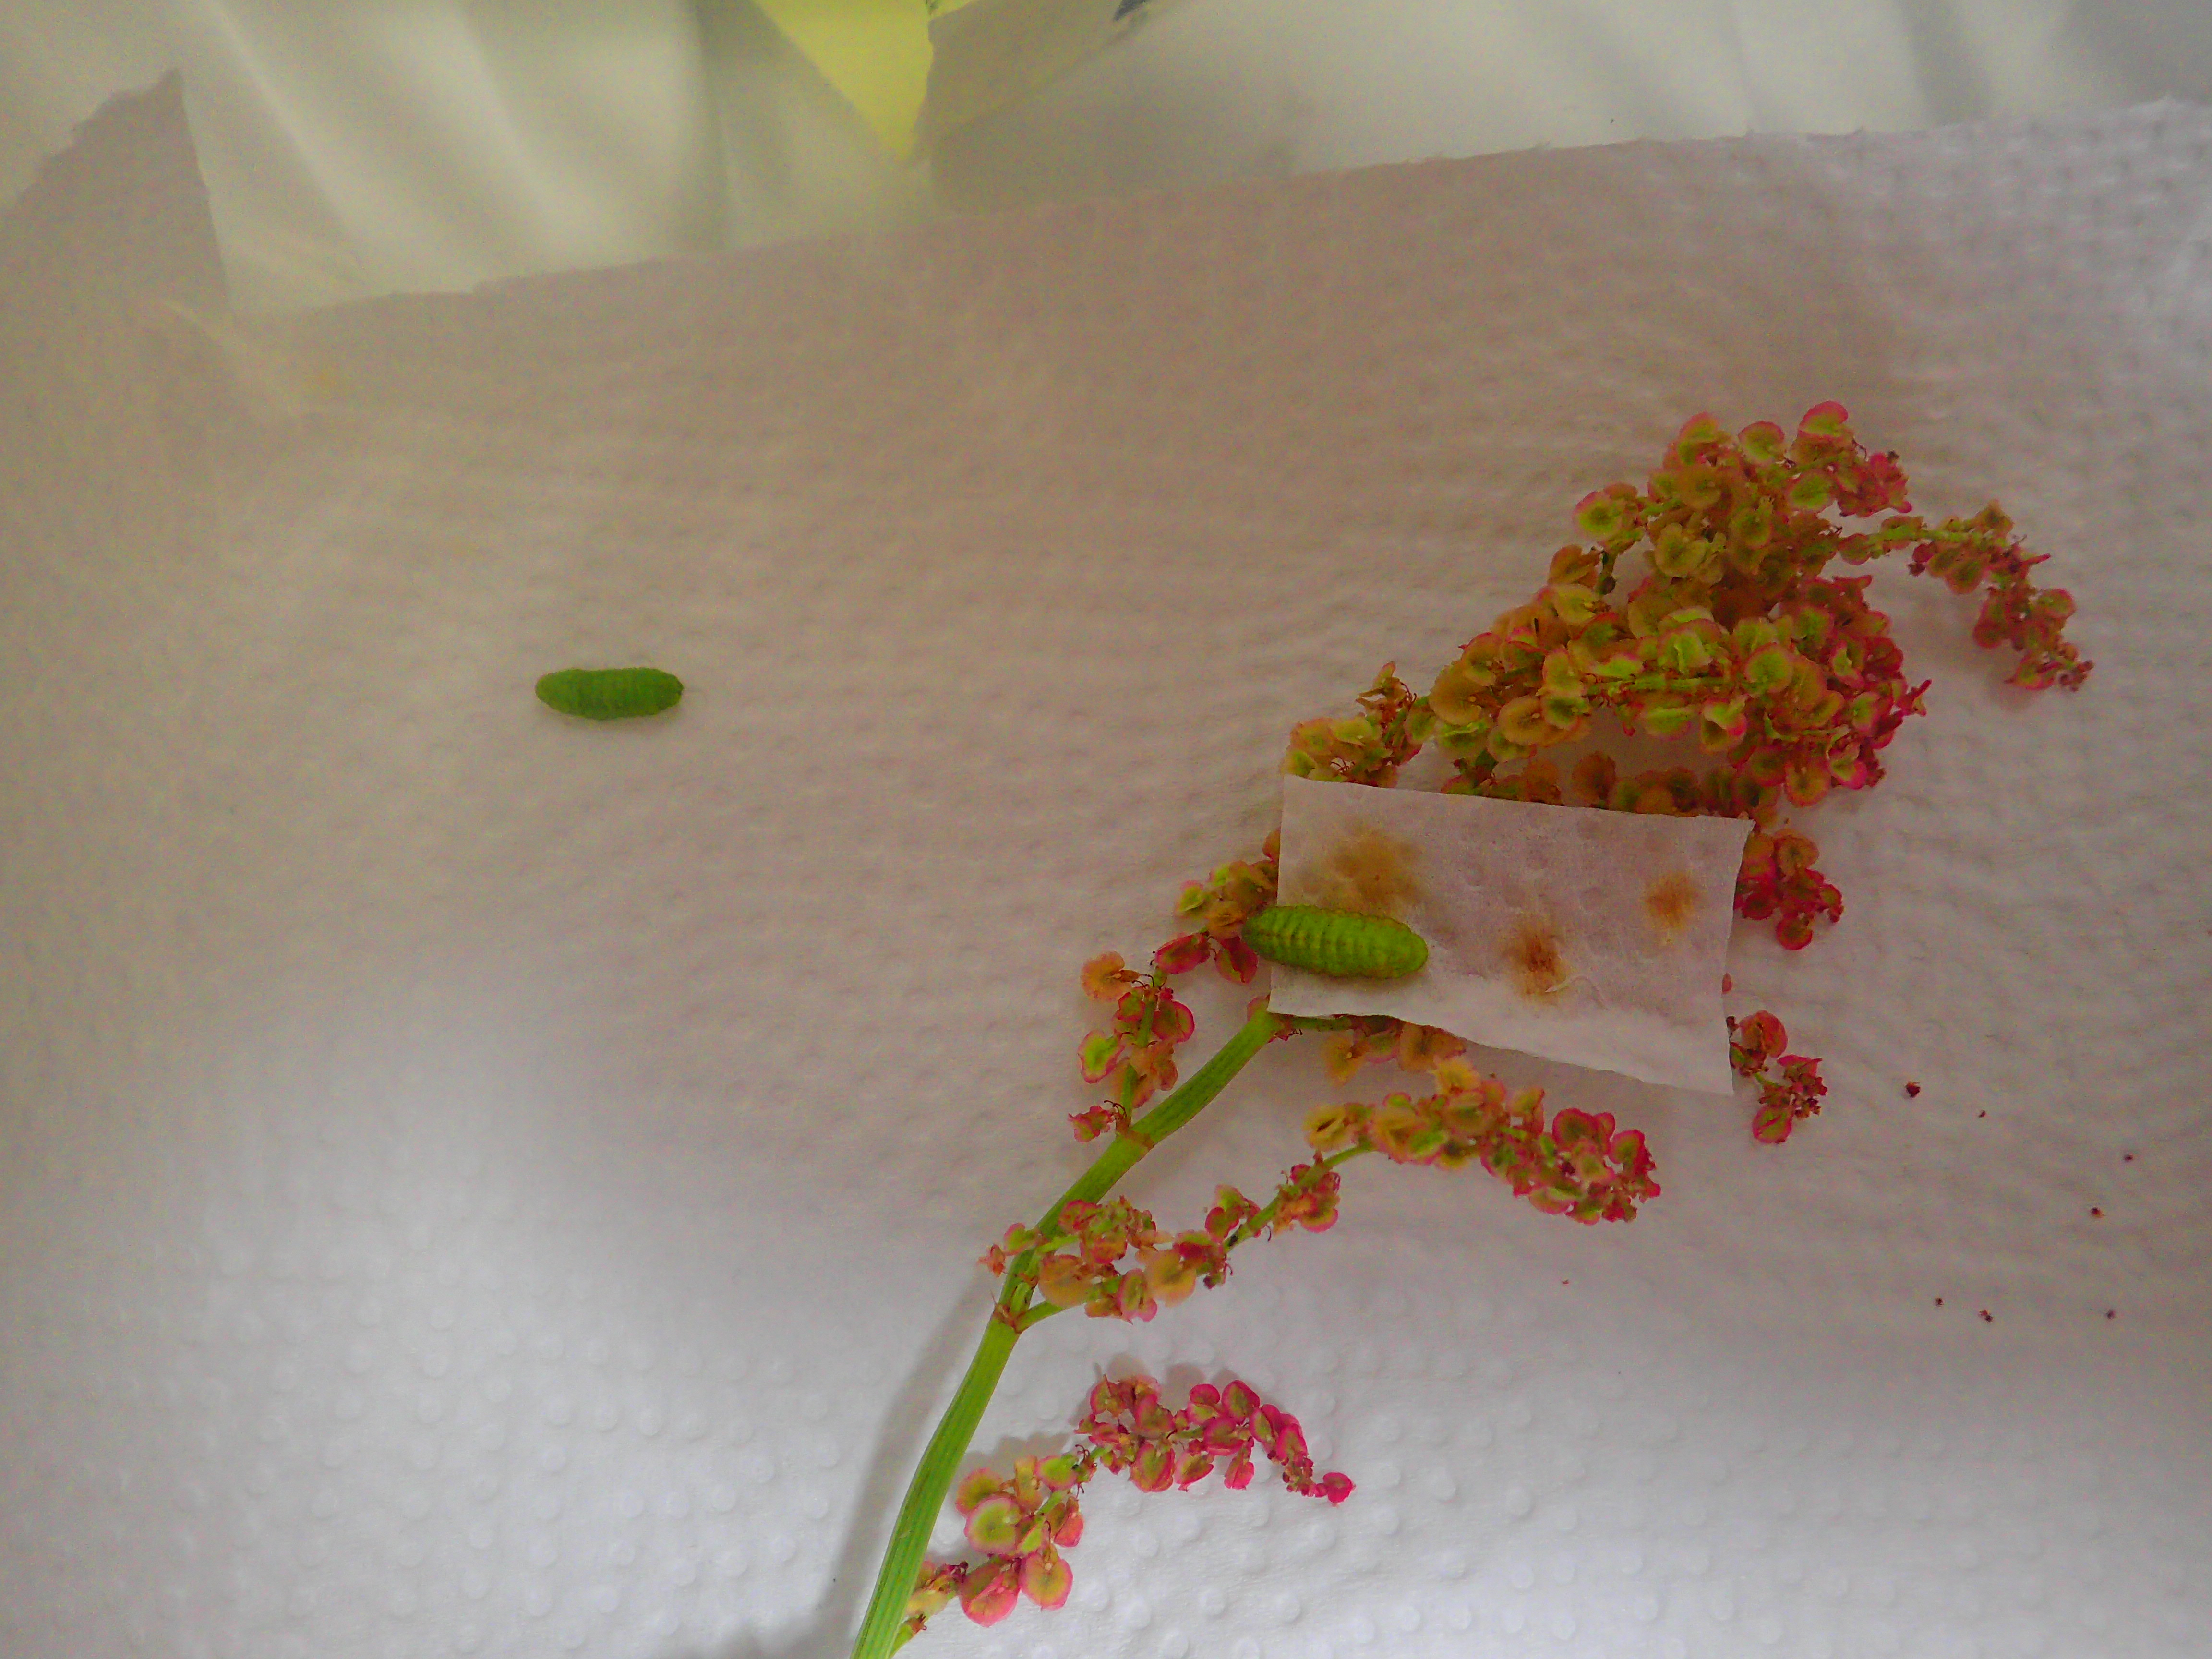
\includegraphics[width=5cm]{photo3/LarvaAwayFromFeed.JPG}
  \end{center}
  \caption{幼虫が食草から離れようとする}
  \label{pic-LarvaAwayFromFeed}
\end{figure}
この動作がなんなのかわからないが, 高熱で脳がやられたか, 何かの予兆かだろう. 
幼虫3, 4はあいかわらずもりもり食べている. この2匹は確実に蝶にしたい. 

\section{5/16の記録}
\subsection{10時:おそらく死んでいる}
幼虫1, 2とも全く動かない. 幼虫1は色も黒ずんできた. 明日判断しよう. 
幼虫2も, 動きはない. もうダメだと思われる. 

\subsection{15時:蛹になるか}
幼虫3が急にいなくなったと思ったら, キッチンペーパーの裏に移動した. 
何やら縮こまっているので, 前蛹と思われる. 意外と早かった. 

\subsection{22時:前蛹の様子がどうも変}
幼虫3の前蛹が, 異様に小さい. また, この状態に入ってから変化がなさすぎるのと, 変な色に変化してきた. 
具体的には黄色がかかっている. さらに, 片方だけに, 黒い大きな斑点が見られる. 
寄生されている可能性が高い. やはり野外で捕獲した幼虫はこんなものか. 
\begin{figure}[htbp]
  \begin{center}
    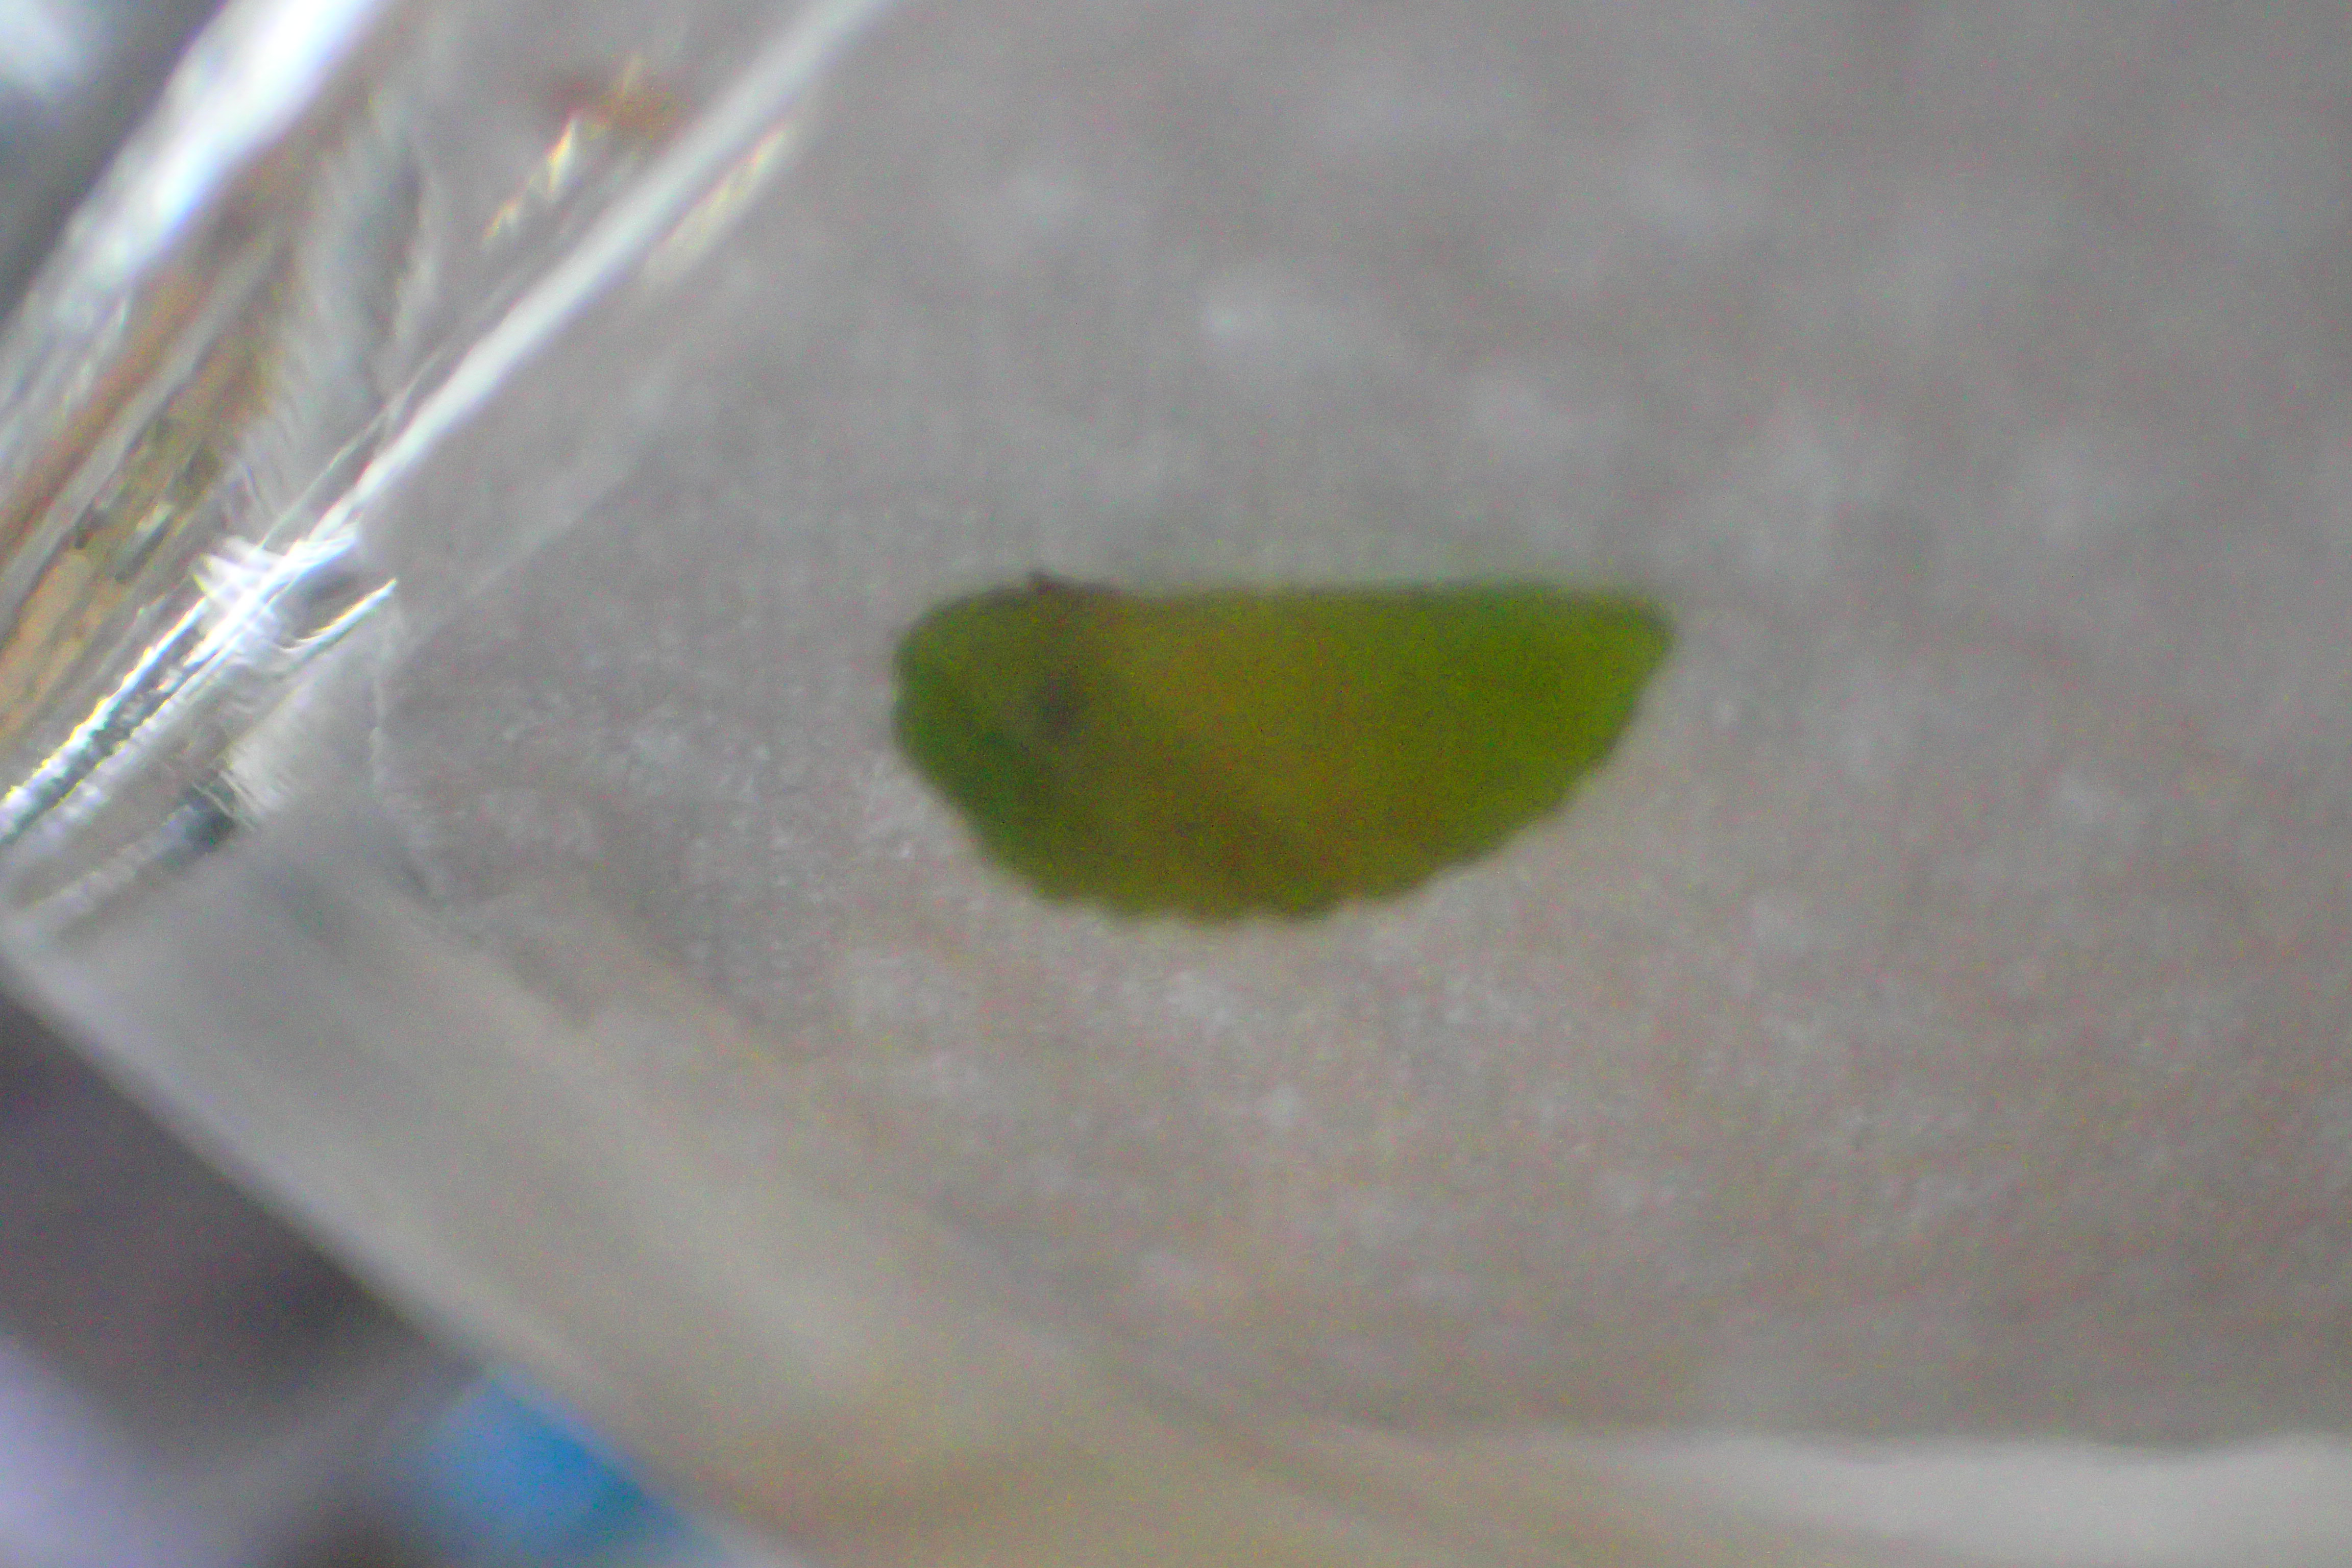
\includegraphics[width=5cm]{photo3/Larva4_prePupa.JPG}
  \end{center}
  \caption{前蛹が寄生されている可能性}
\end{figure}

\section{5/17の記録}
\subsection{12時:死亡判断}
もう完全に幼虫1, 2は動かないし, 明らかに干からびている. 死亡と判断した.

\begin{figure}[htbp]
  \begin{minipage}{0.5\hsize}
    \begin{center}
      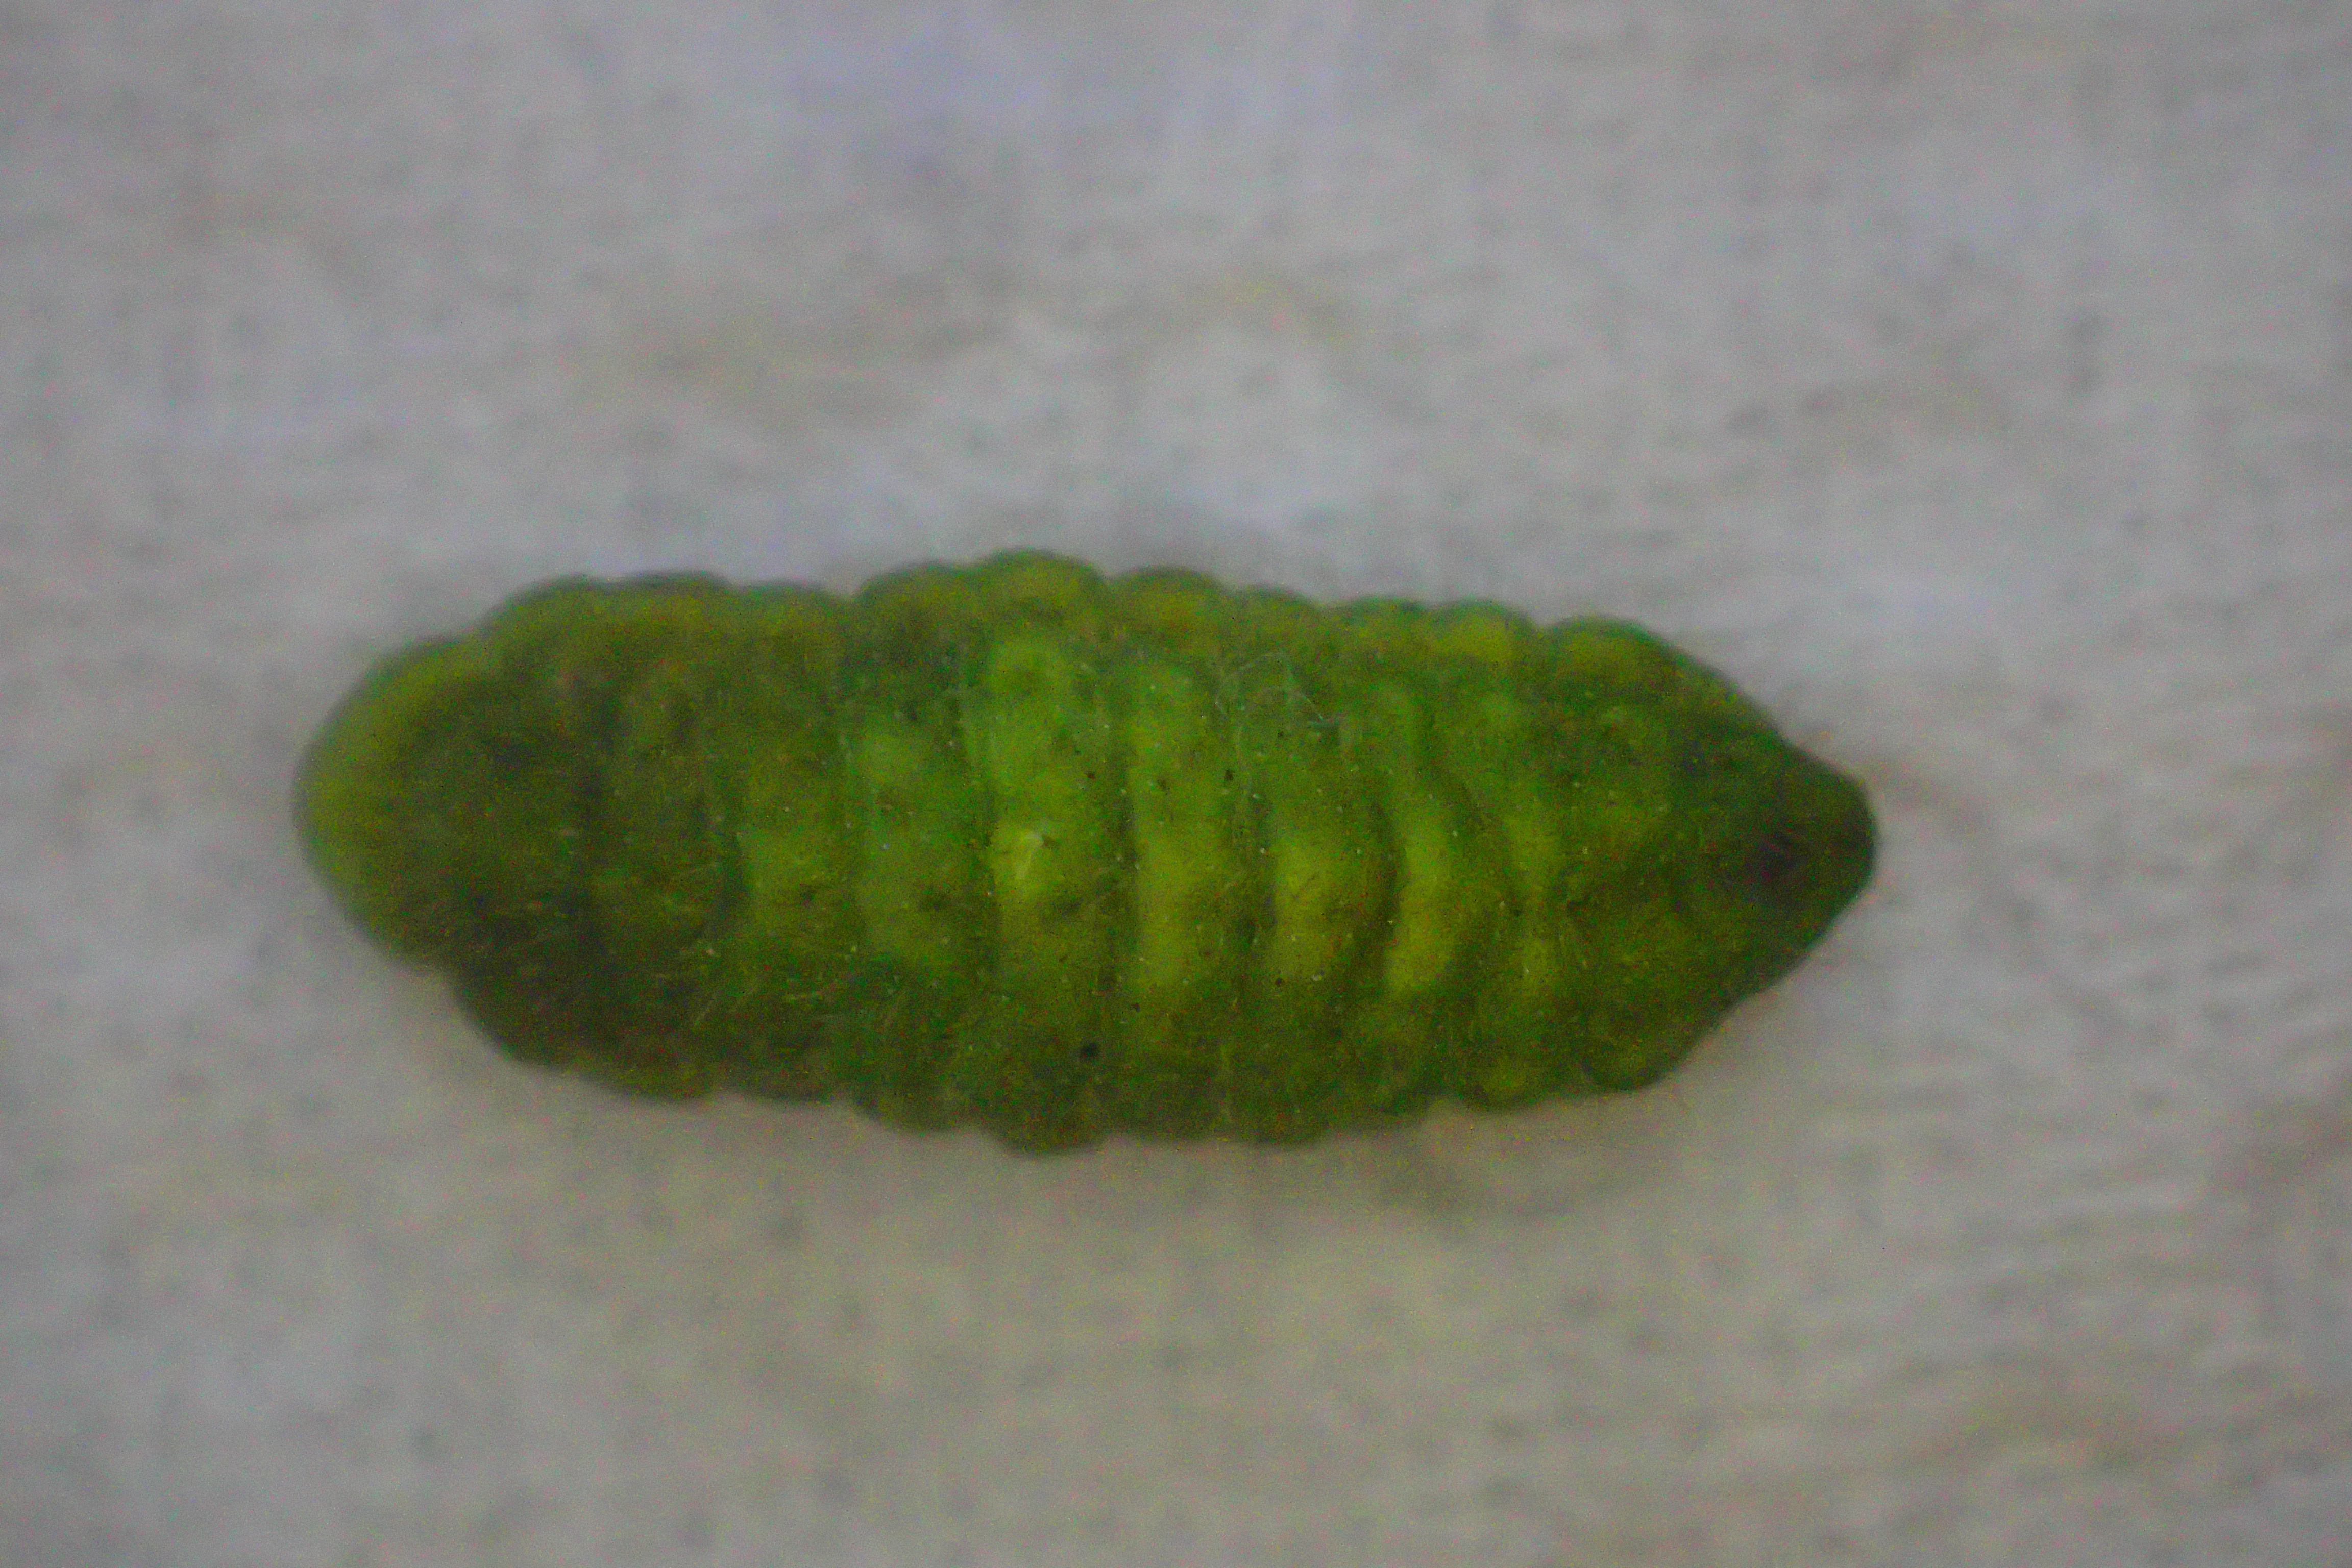
\includegraphics[width=5cm]{photo4/Larva1Dead.JPG}
    \end{center}
    \caption{幼虫1の死亡}
    \label{Larba1Dead}
  \end{minipage}
  \begin{minipage}{0.5\hsize}
    \begin{center}
      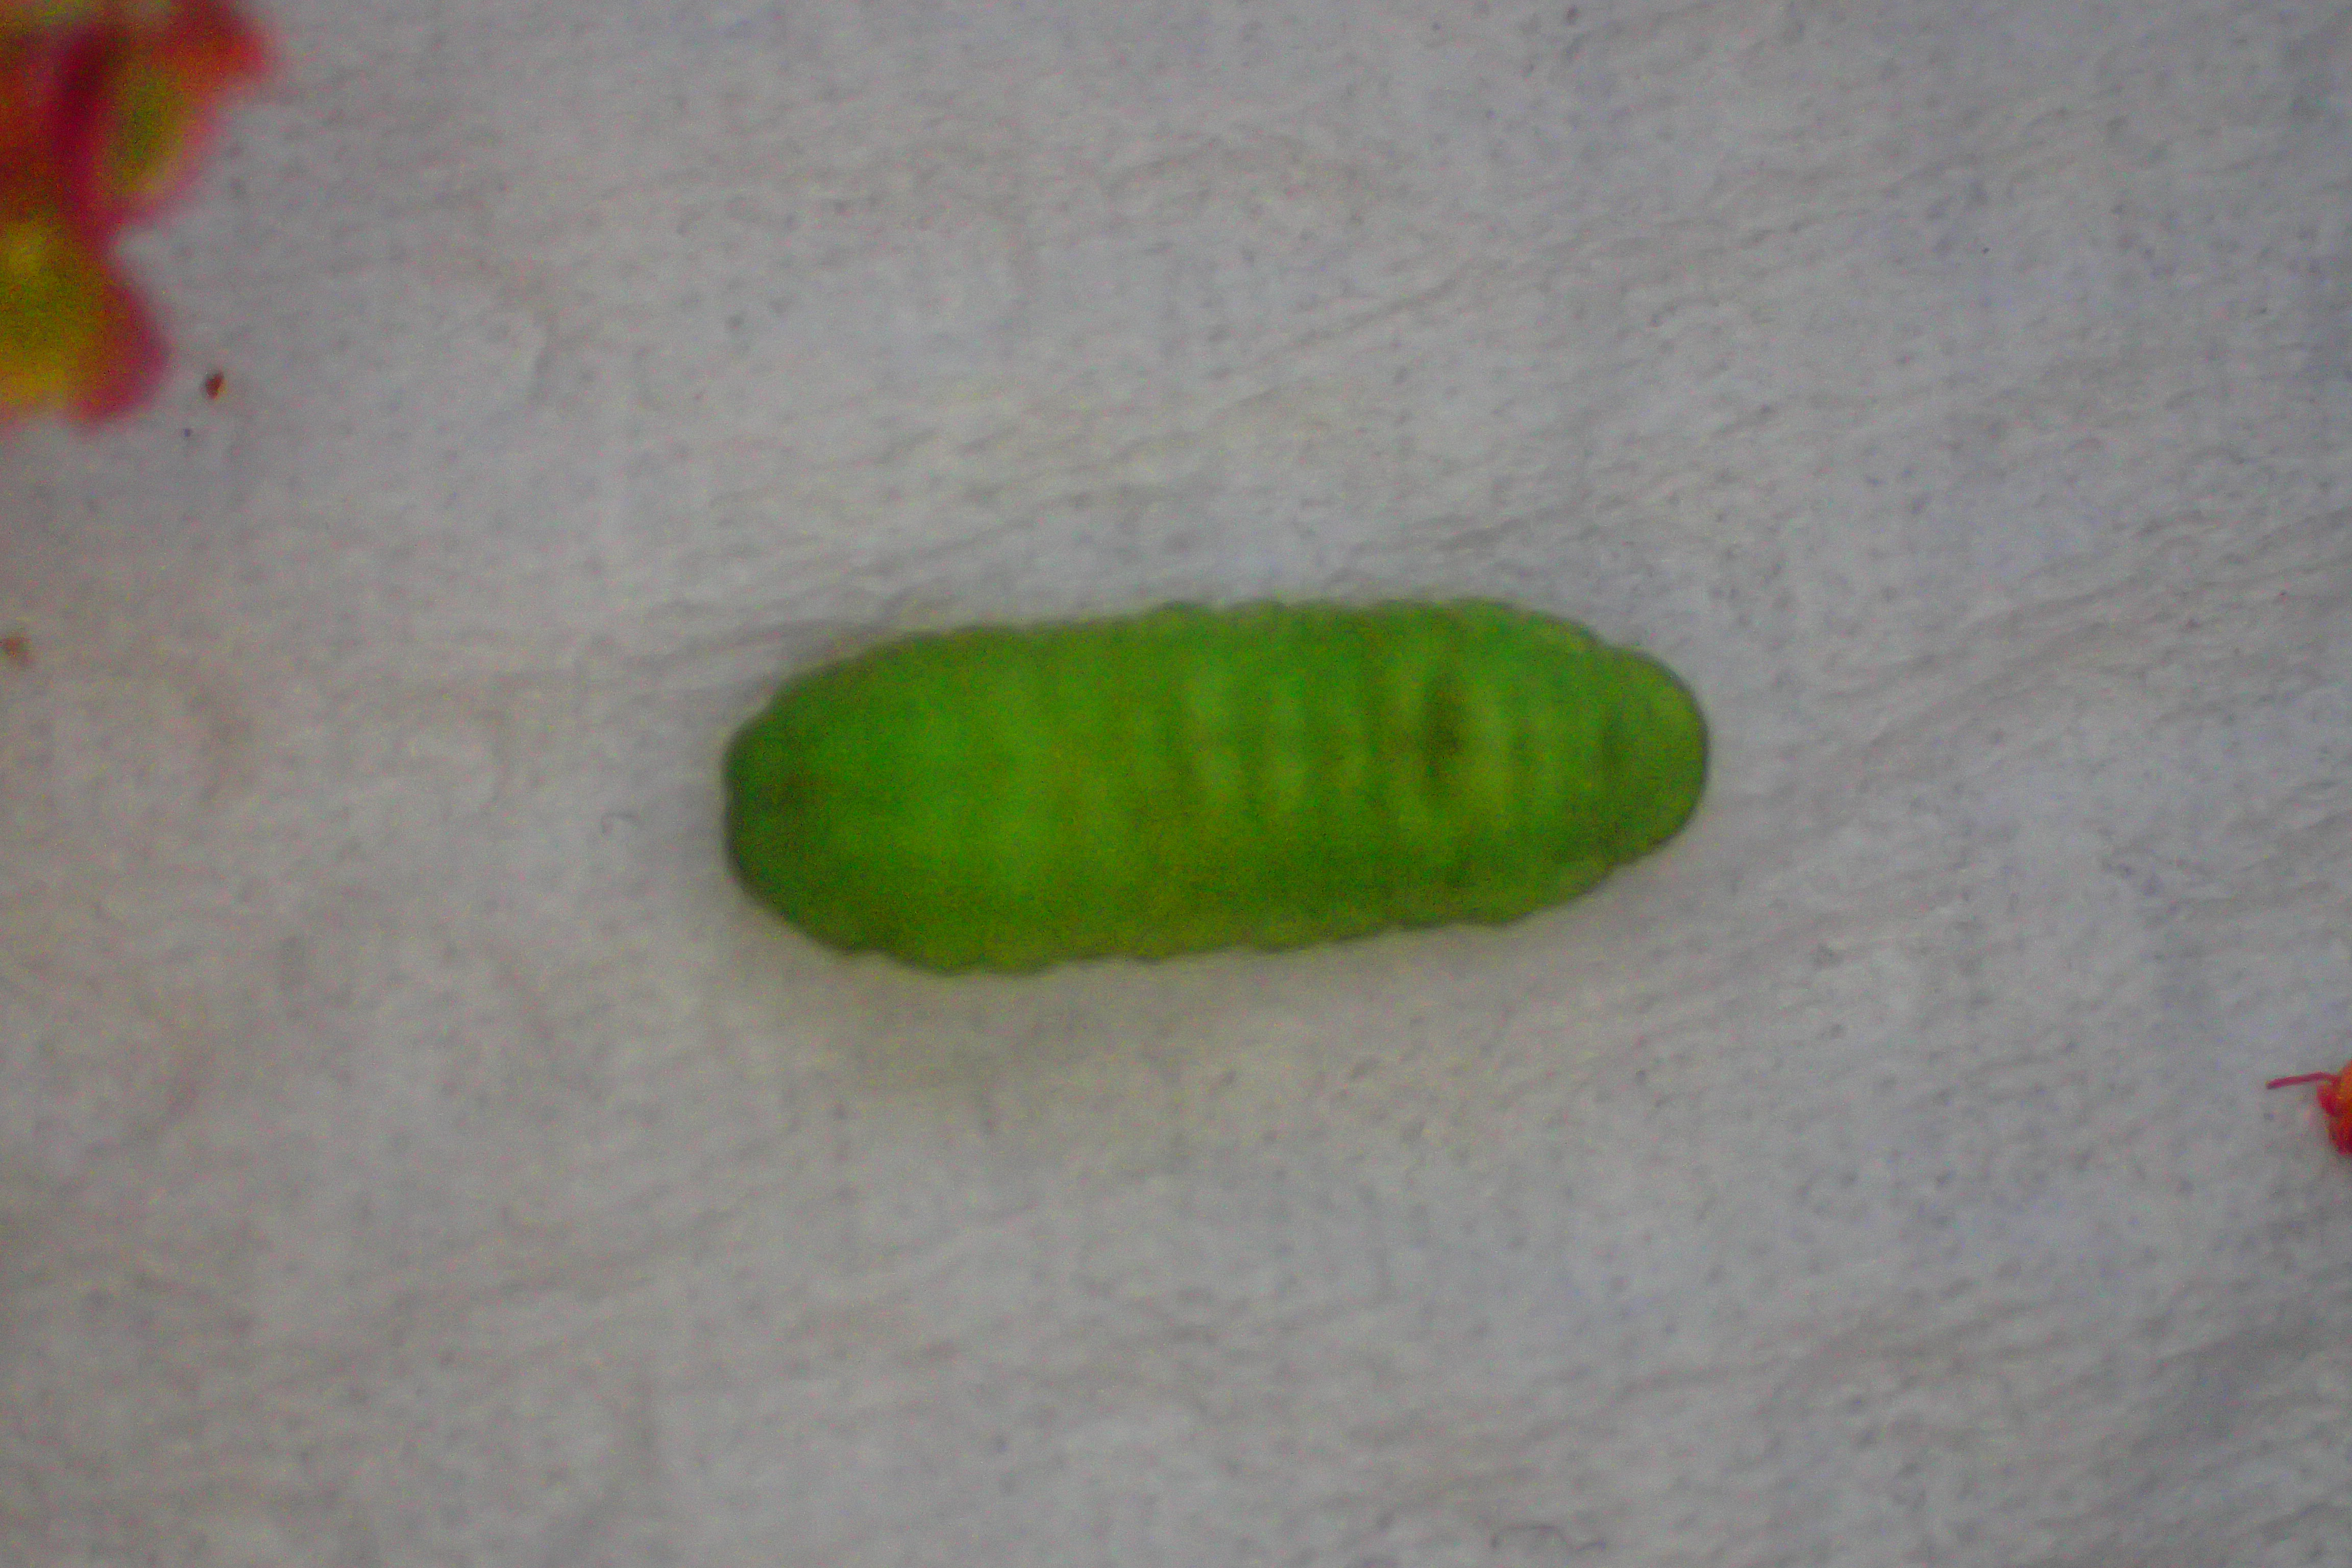
\includegraphics[width=5cm]{photo4/Larva2Dead.JPG}
    \end{center}
    \caption{幼虫2の死亡}
    \label{Larba2Dead}
  \end{minipage}
\end{figure}

幼虫3の前蛹は, ますます色が黄色がかってきており, 黒い斑点も大きくなってきた. 
おそらく, 中にハチ, もしくはハエがいる. 

\begin{figure}[htbp]
  \begin{center}
    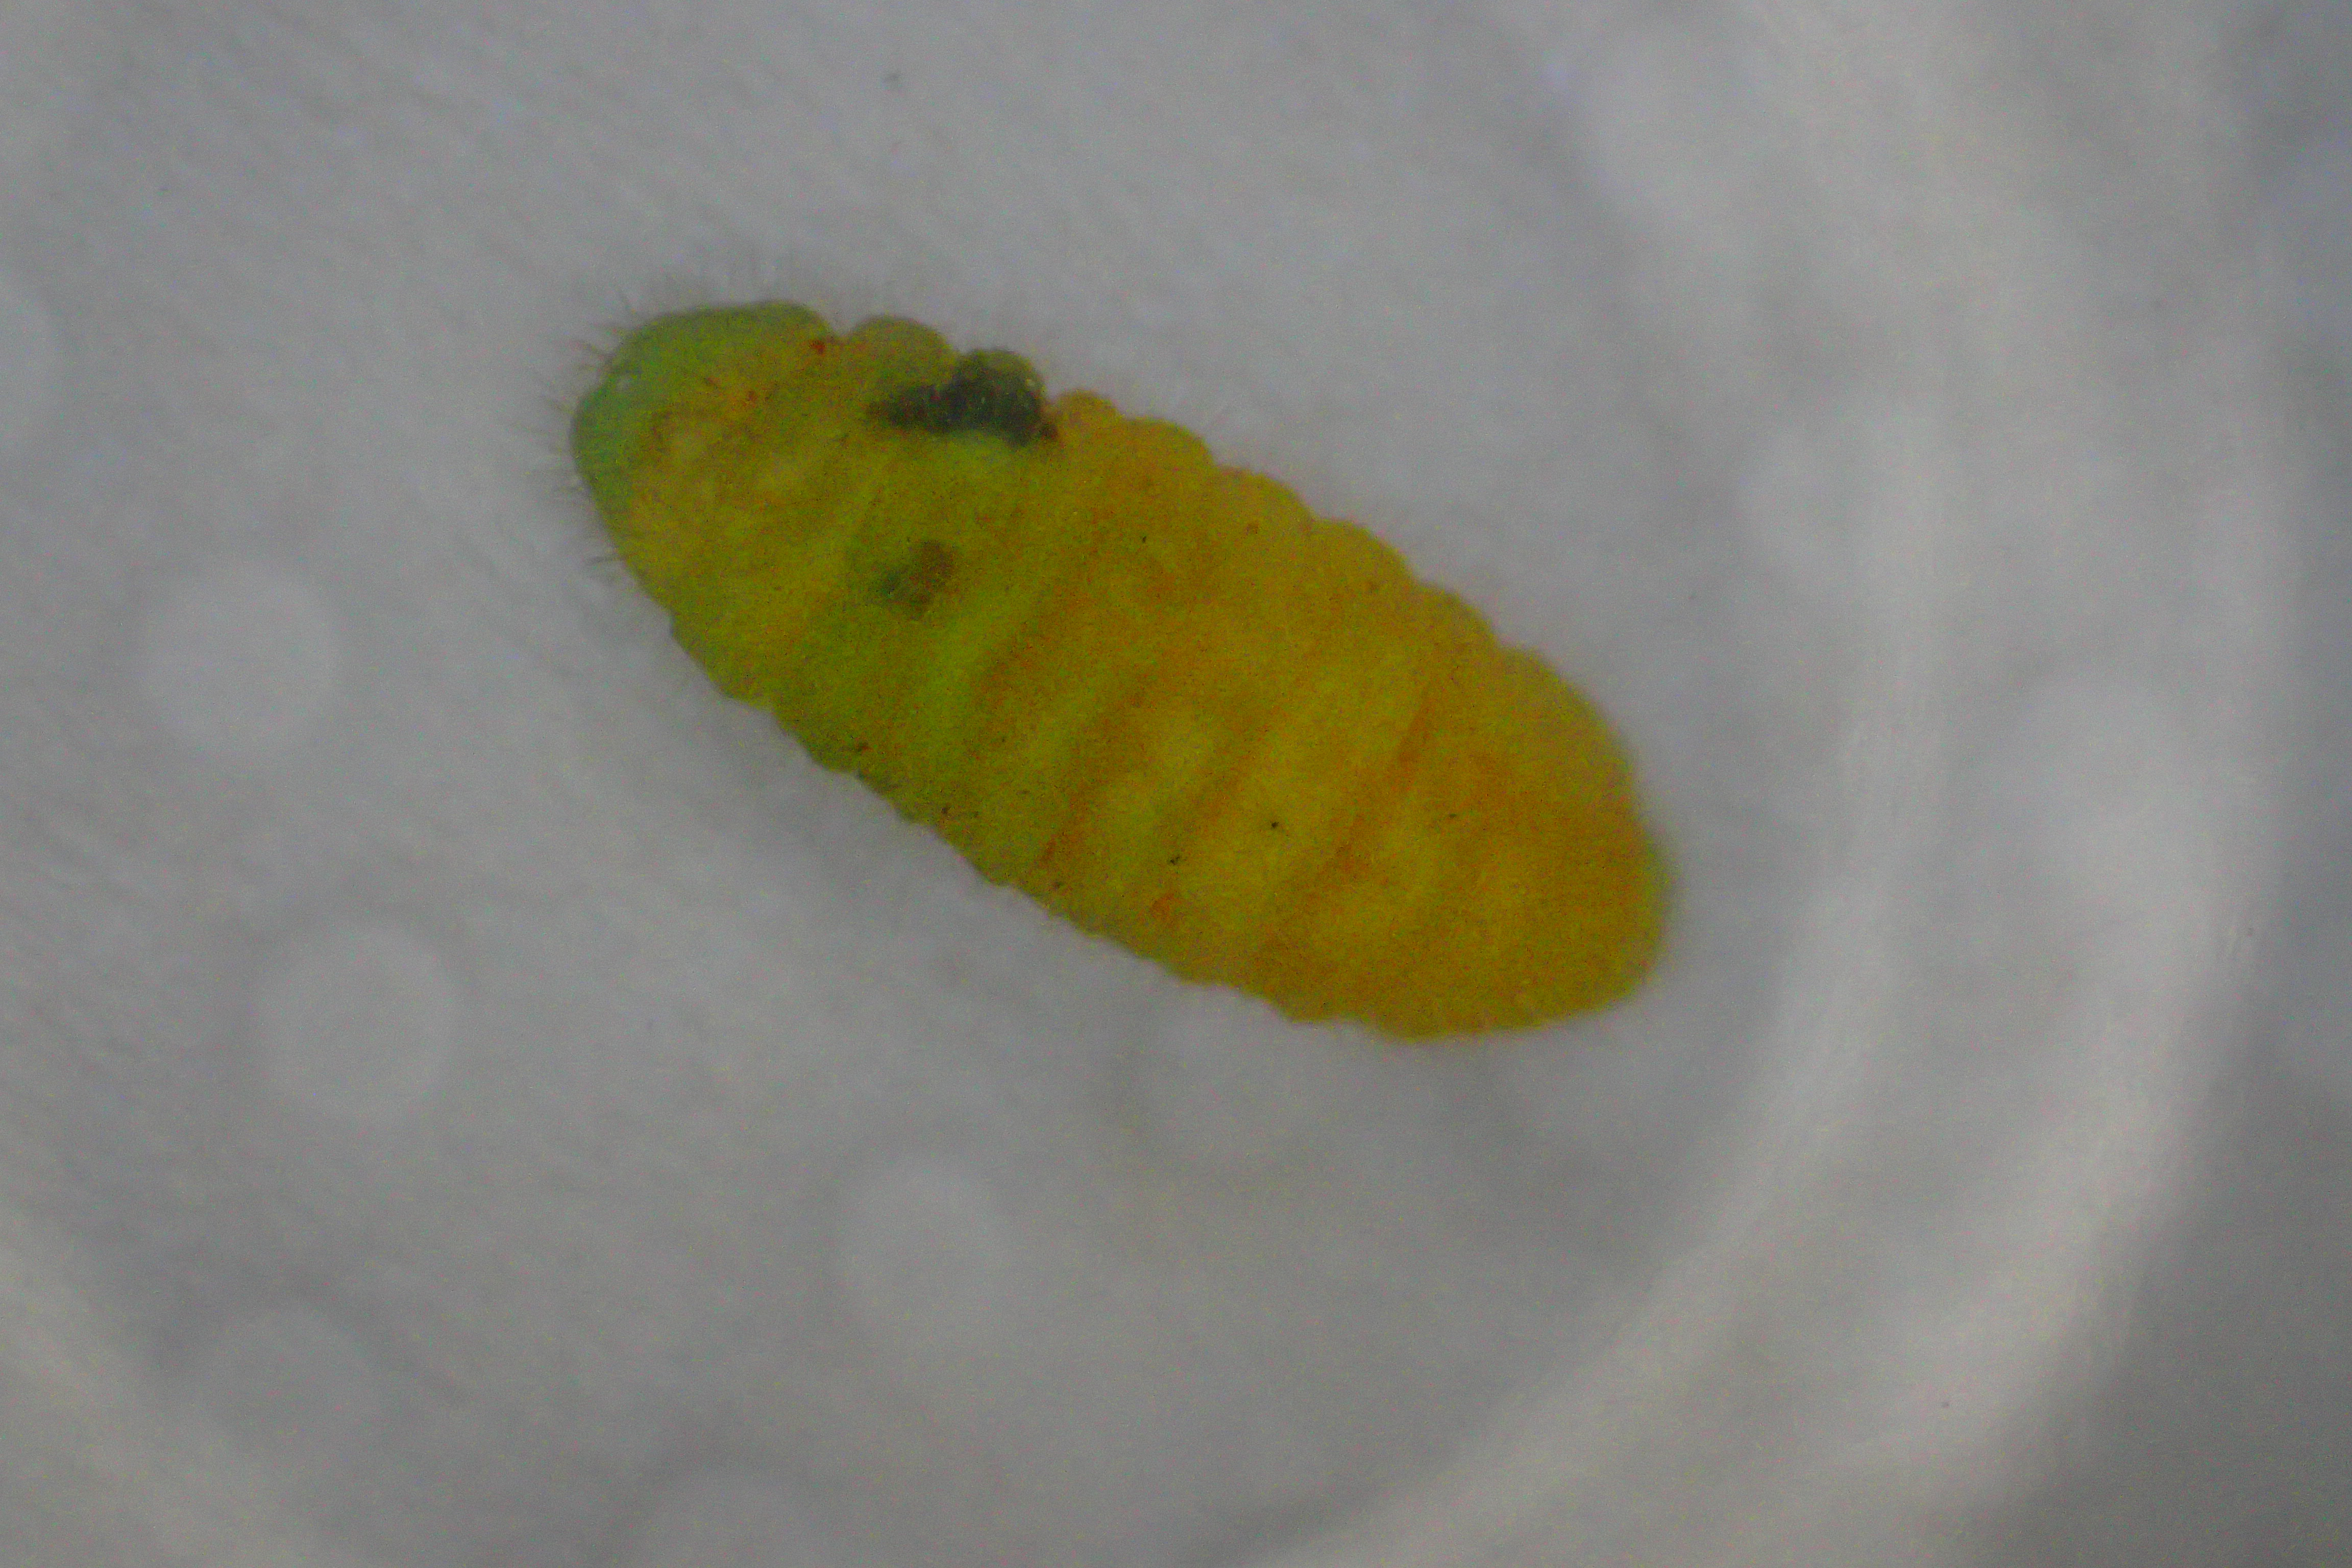
\includegraphics[width=5cm]{photo4/pupa_parasited.JPG}
  \end{center}
  \caption{前蛹が黄色く変色し, 黒い斑点が目立つようになってきた}
\end{figure}

\subsection{15時:2匹確保}
四季の森公園にて, 計3匹の幼虫を見つけた. 一匹はおそらく終齢(以後幼虫5), もう2匹は2齢程度. 2齢のうち1匹は, 捕獲中に落下してしまったので, 計2匹捕獲. 終齢は, 例のごとく花に貪りついていたが, 2齢の幼虫(以後幼虫6)はどちらも割と苗の中段付近の枝で見つかった. 
割と, 若い幼虫のほうが, 葉裏にいるのかもしれない. 
\begin{figure}[htbp]
  \begin{minipage}{0.5\hsize}
    \begin{center}
      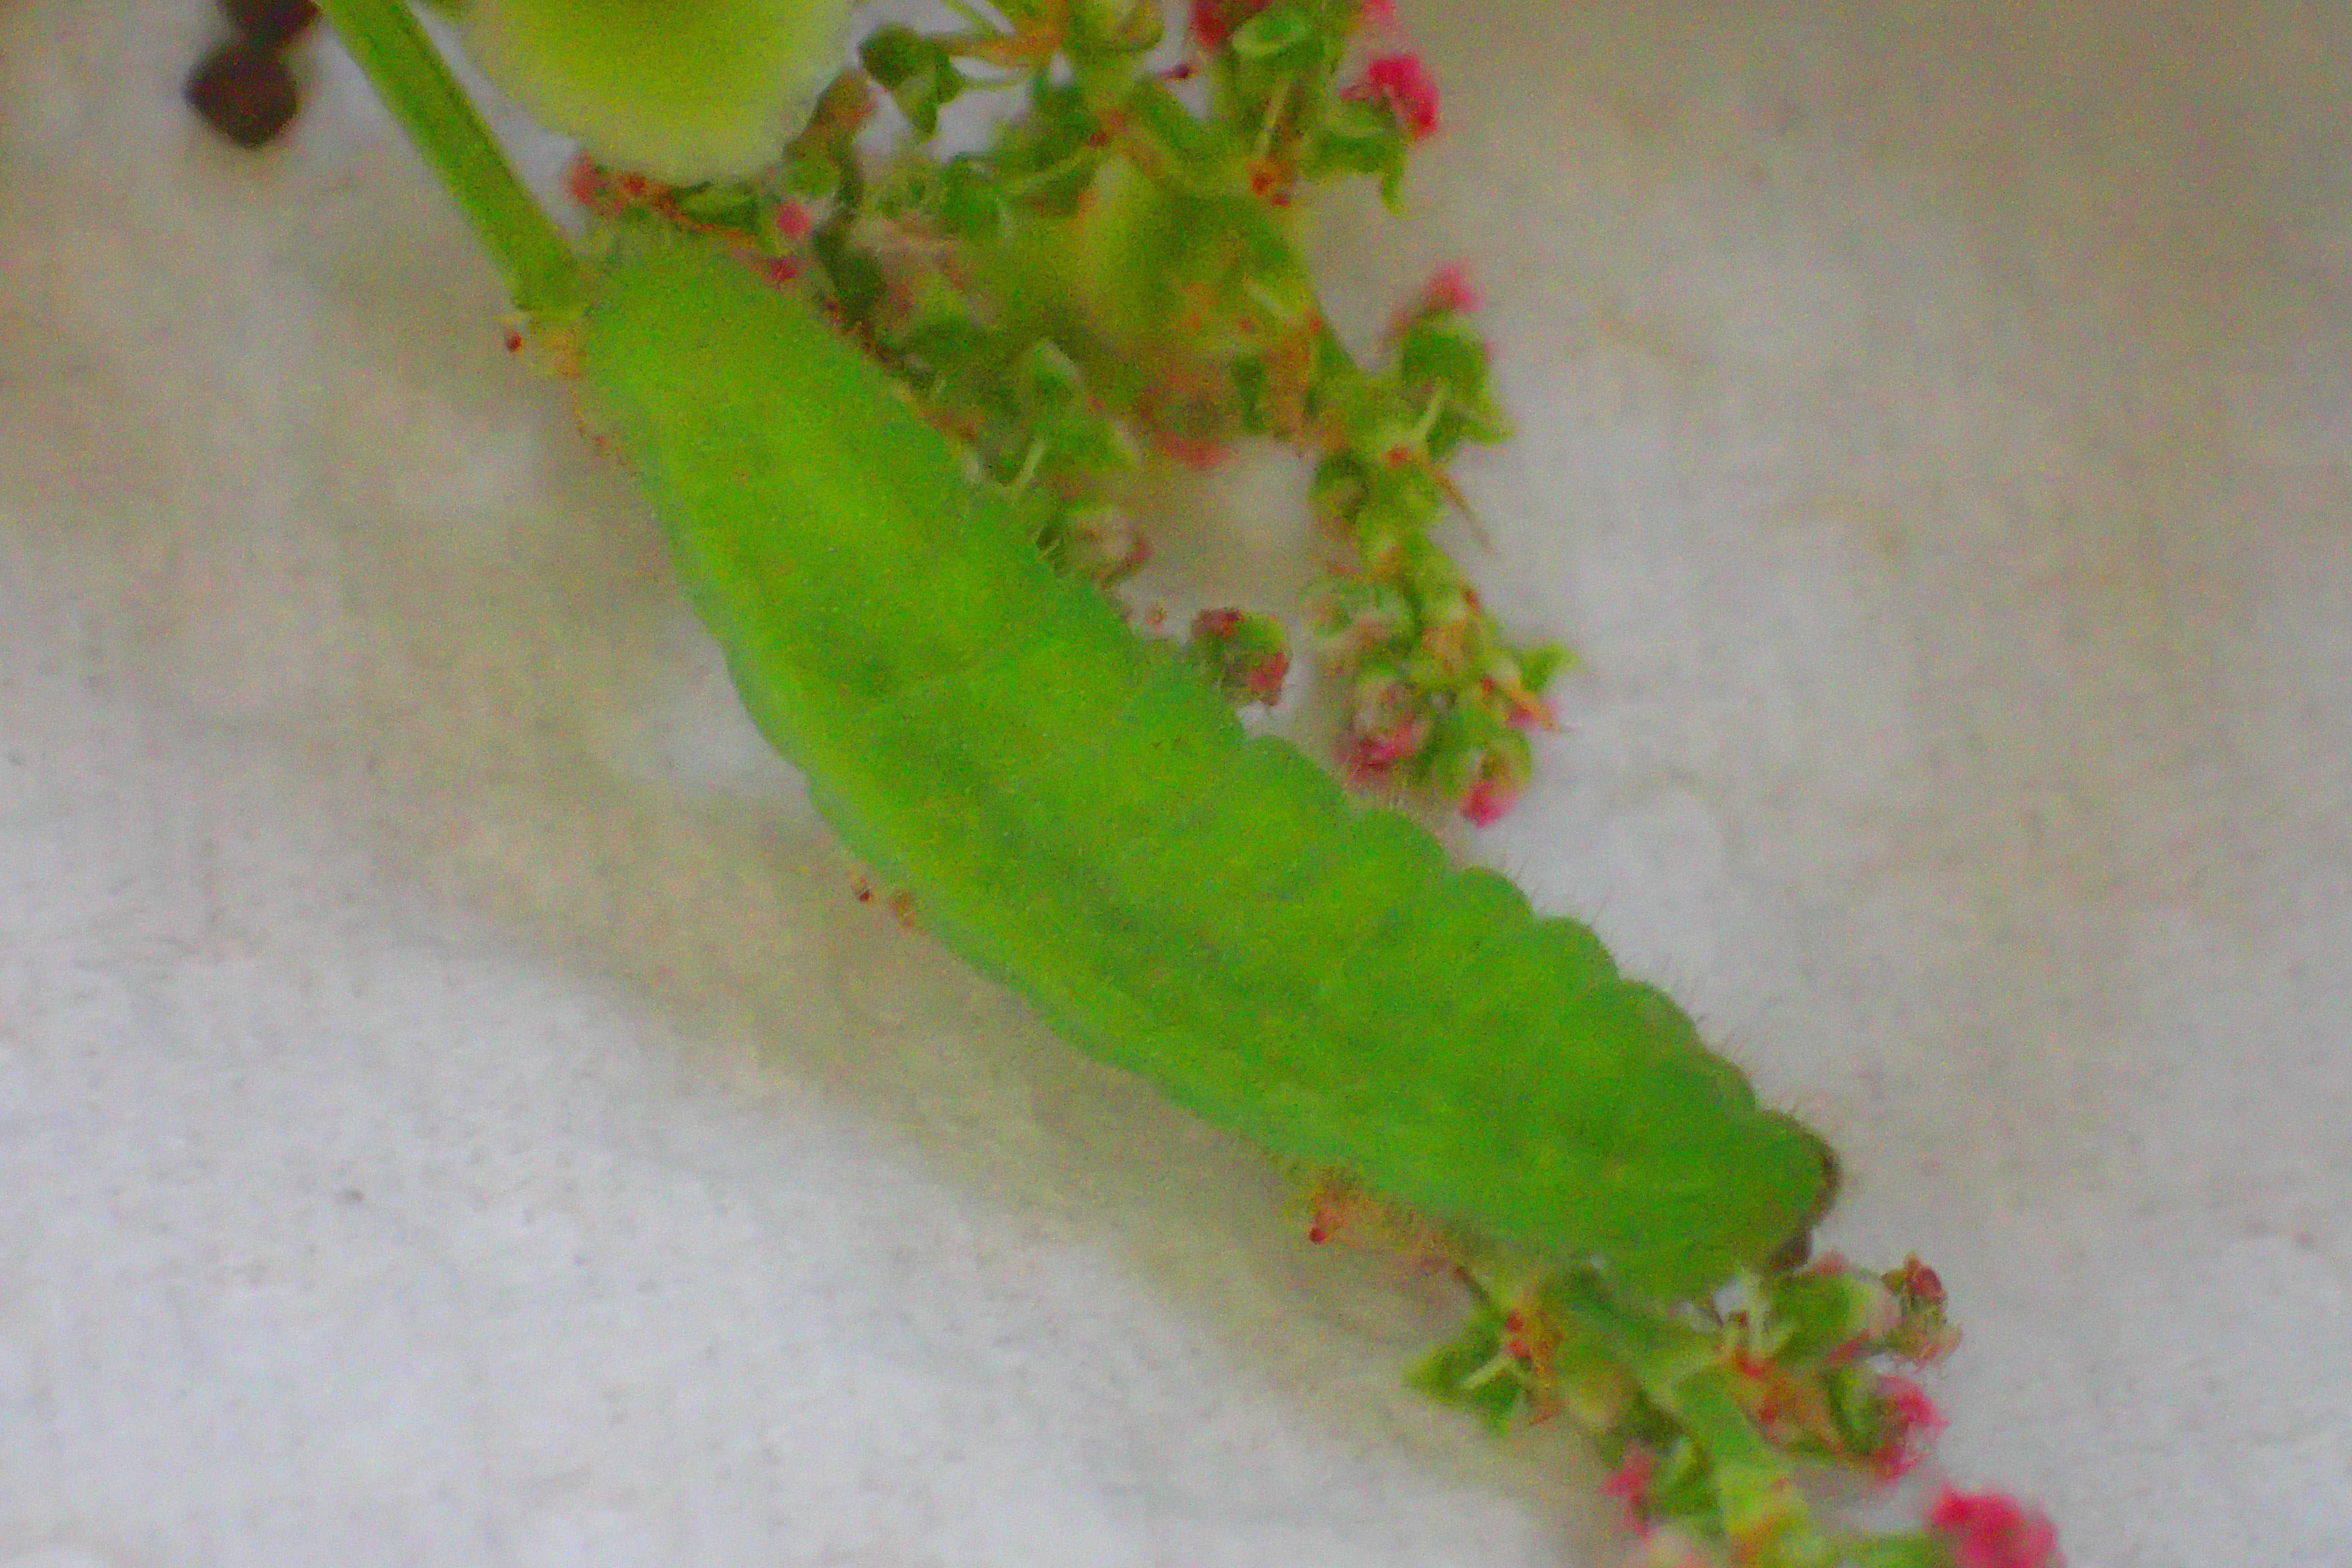
\includegraphics[width=5cm]{photo4/Larva5.JPG}
    \end{center}
    \caption{幼虫5}
  \end{minipage}
  \begin{minipage}{0.5\hsize}
    \begin{center}
      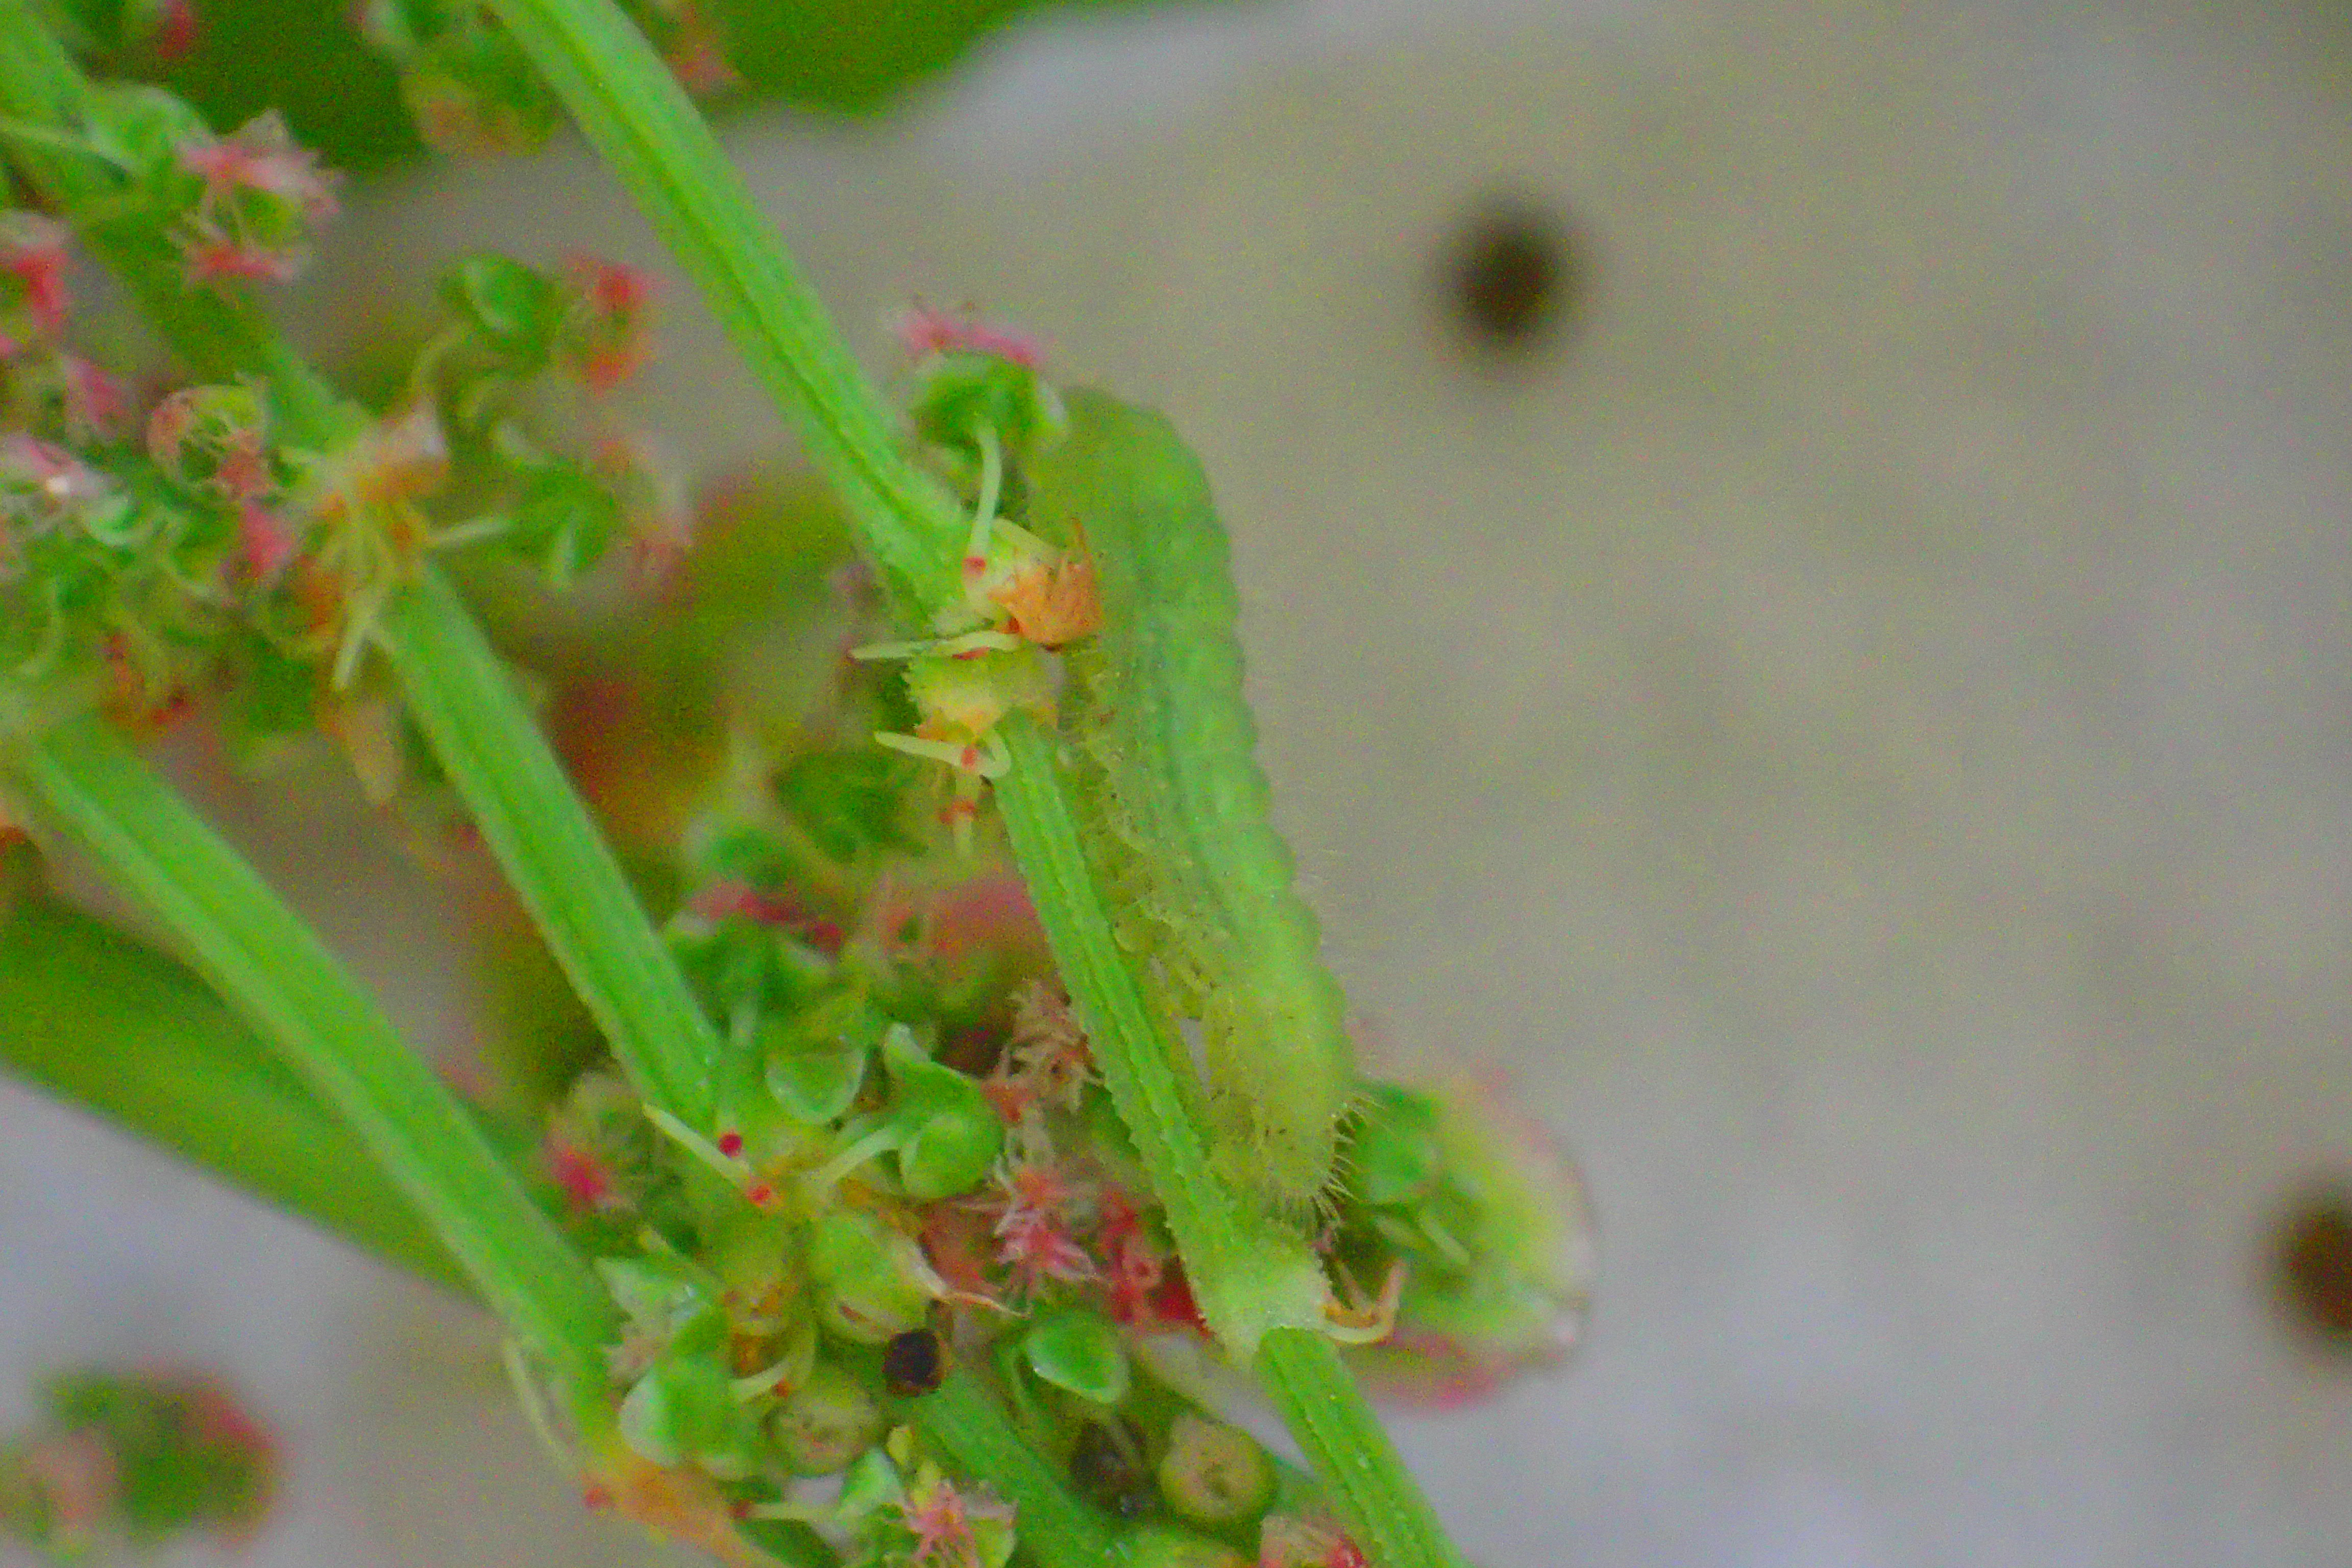
\includegraphics[width=5cm]{photo4/Larva6.JPG}
    \end{center}
    \caption{幼虫6}
  \end{minipage}
\end{figure}

\subsection{16時:蛆虫がでてきた}
幼虫3の前蛹を別ケースに移動しておいたが, ケースを見ると, 黄色い蛆虫が高速に移動していた. 
もう少し気づくのが遅かったら, 家の中を這っていたことだろう. 
案の定, 黒い斑点があったところに穴が空き, 蛆虫が出てきたようだ. 
ハエかハチか, 正体を見極めてもいいが, そこまでするのもケースの無駄なので, 水中で死んでもらうことにした. 
\begin{figure}[htbp]
  \begin{minipage}{0.5\hsize}
    \begin{center}
      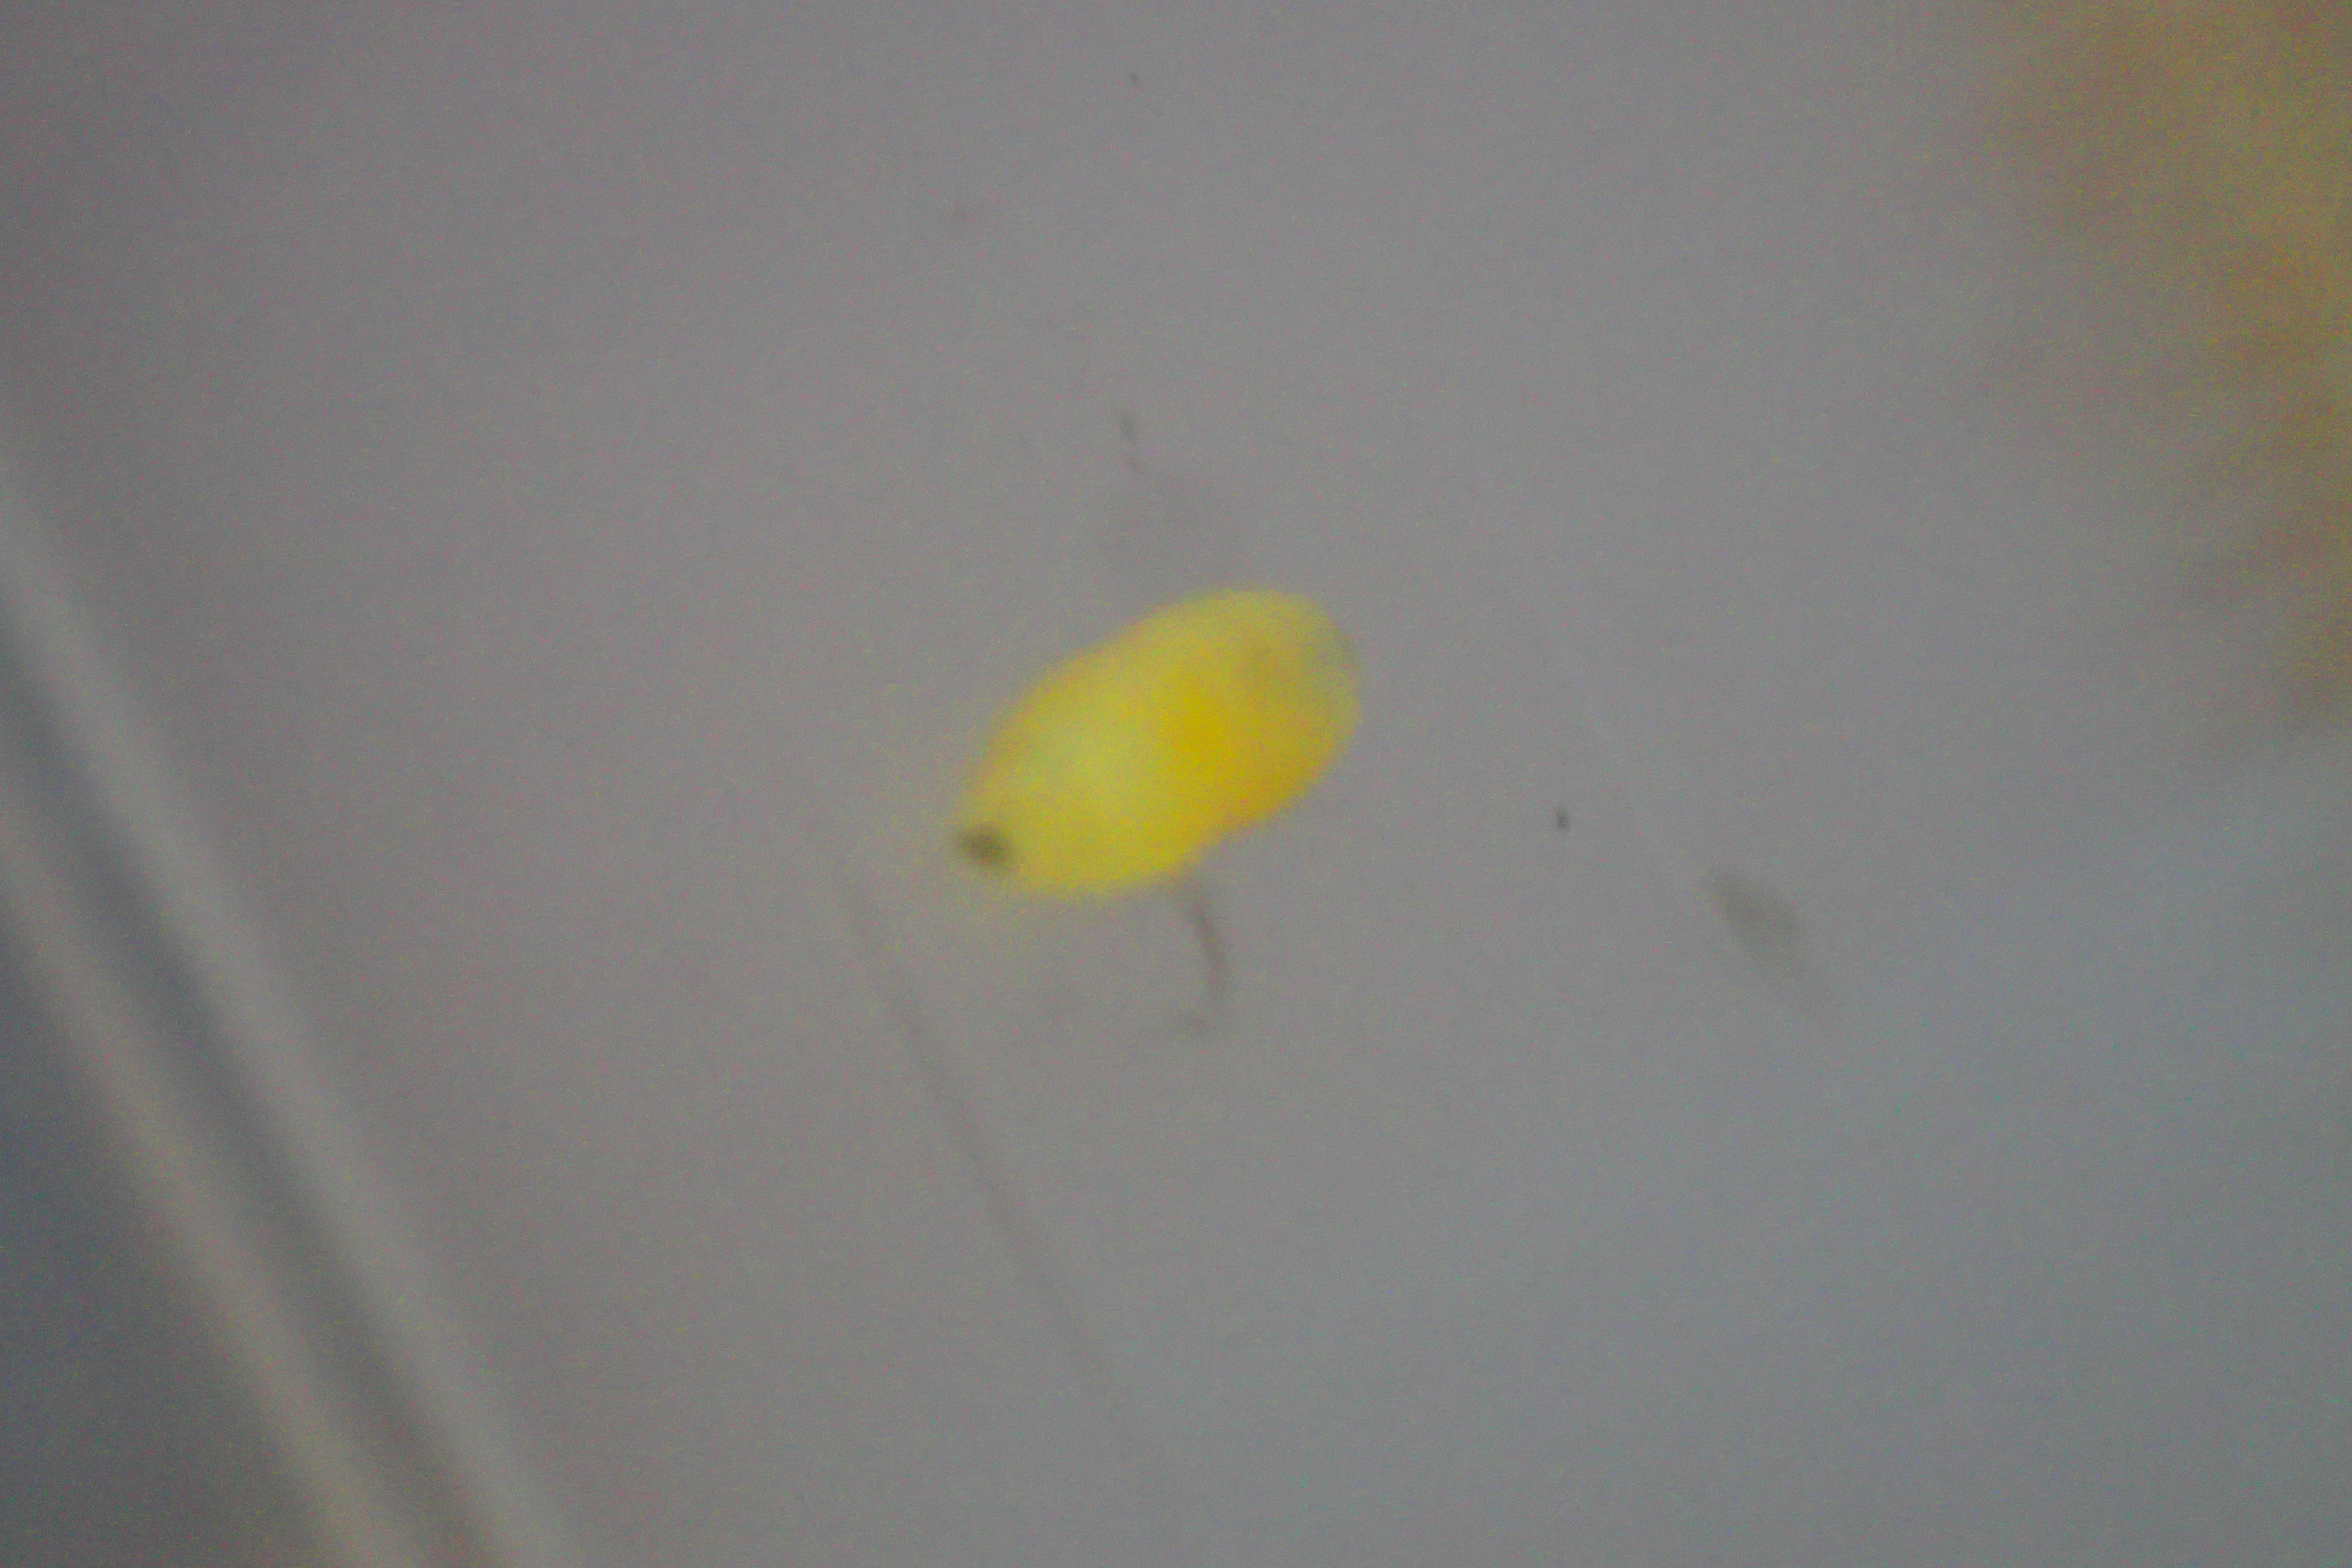
\includegraphics[width=5cm]{photo4/maggot.JPG}
    \end{center}
    \caption{蛆虫}
  \end{minipage}
  \begin{minipage}{0.5\hsize}
    \begin{center}
      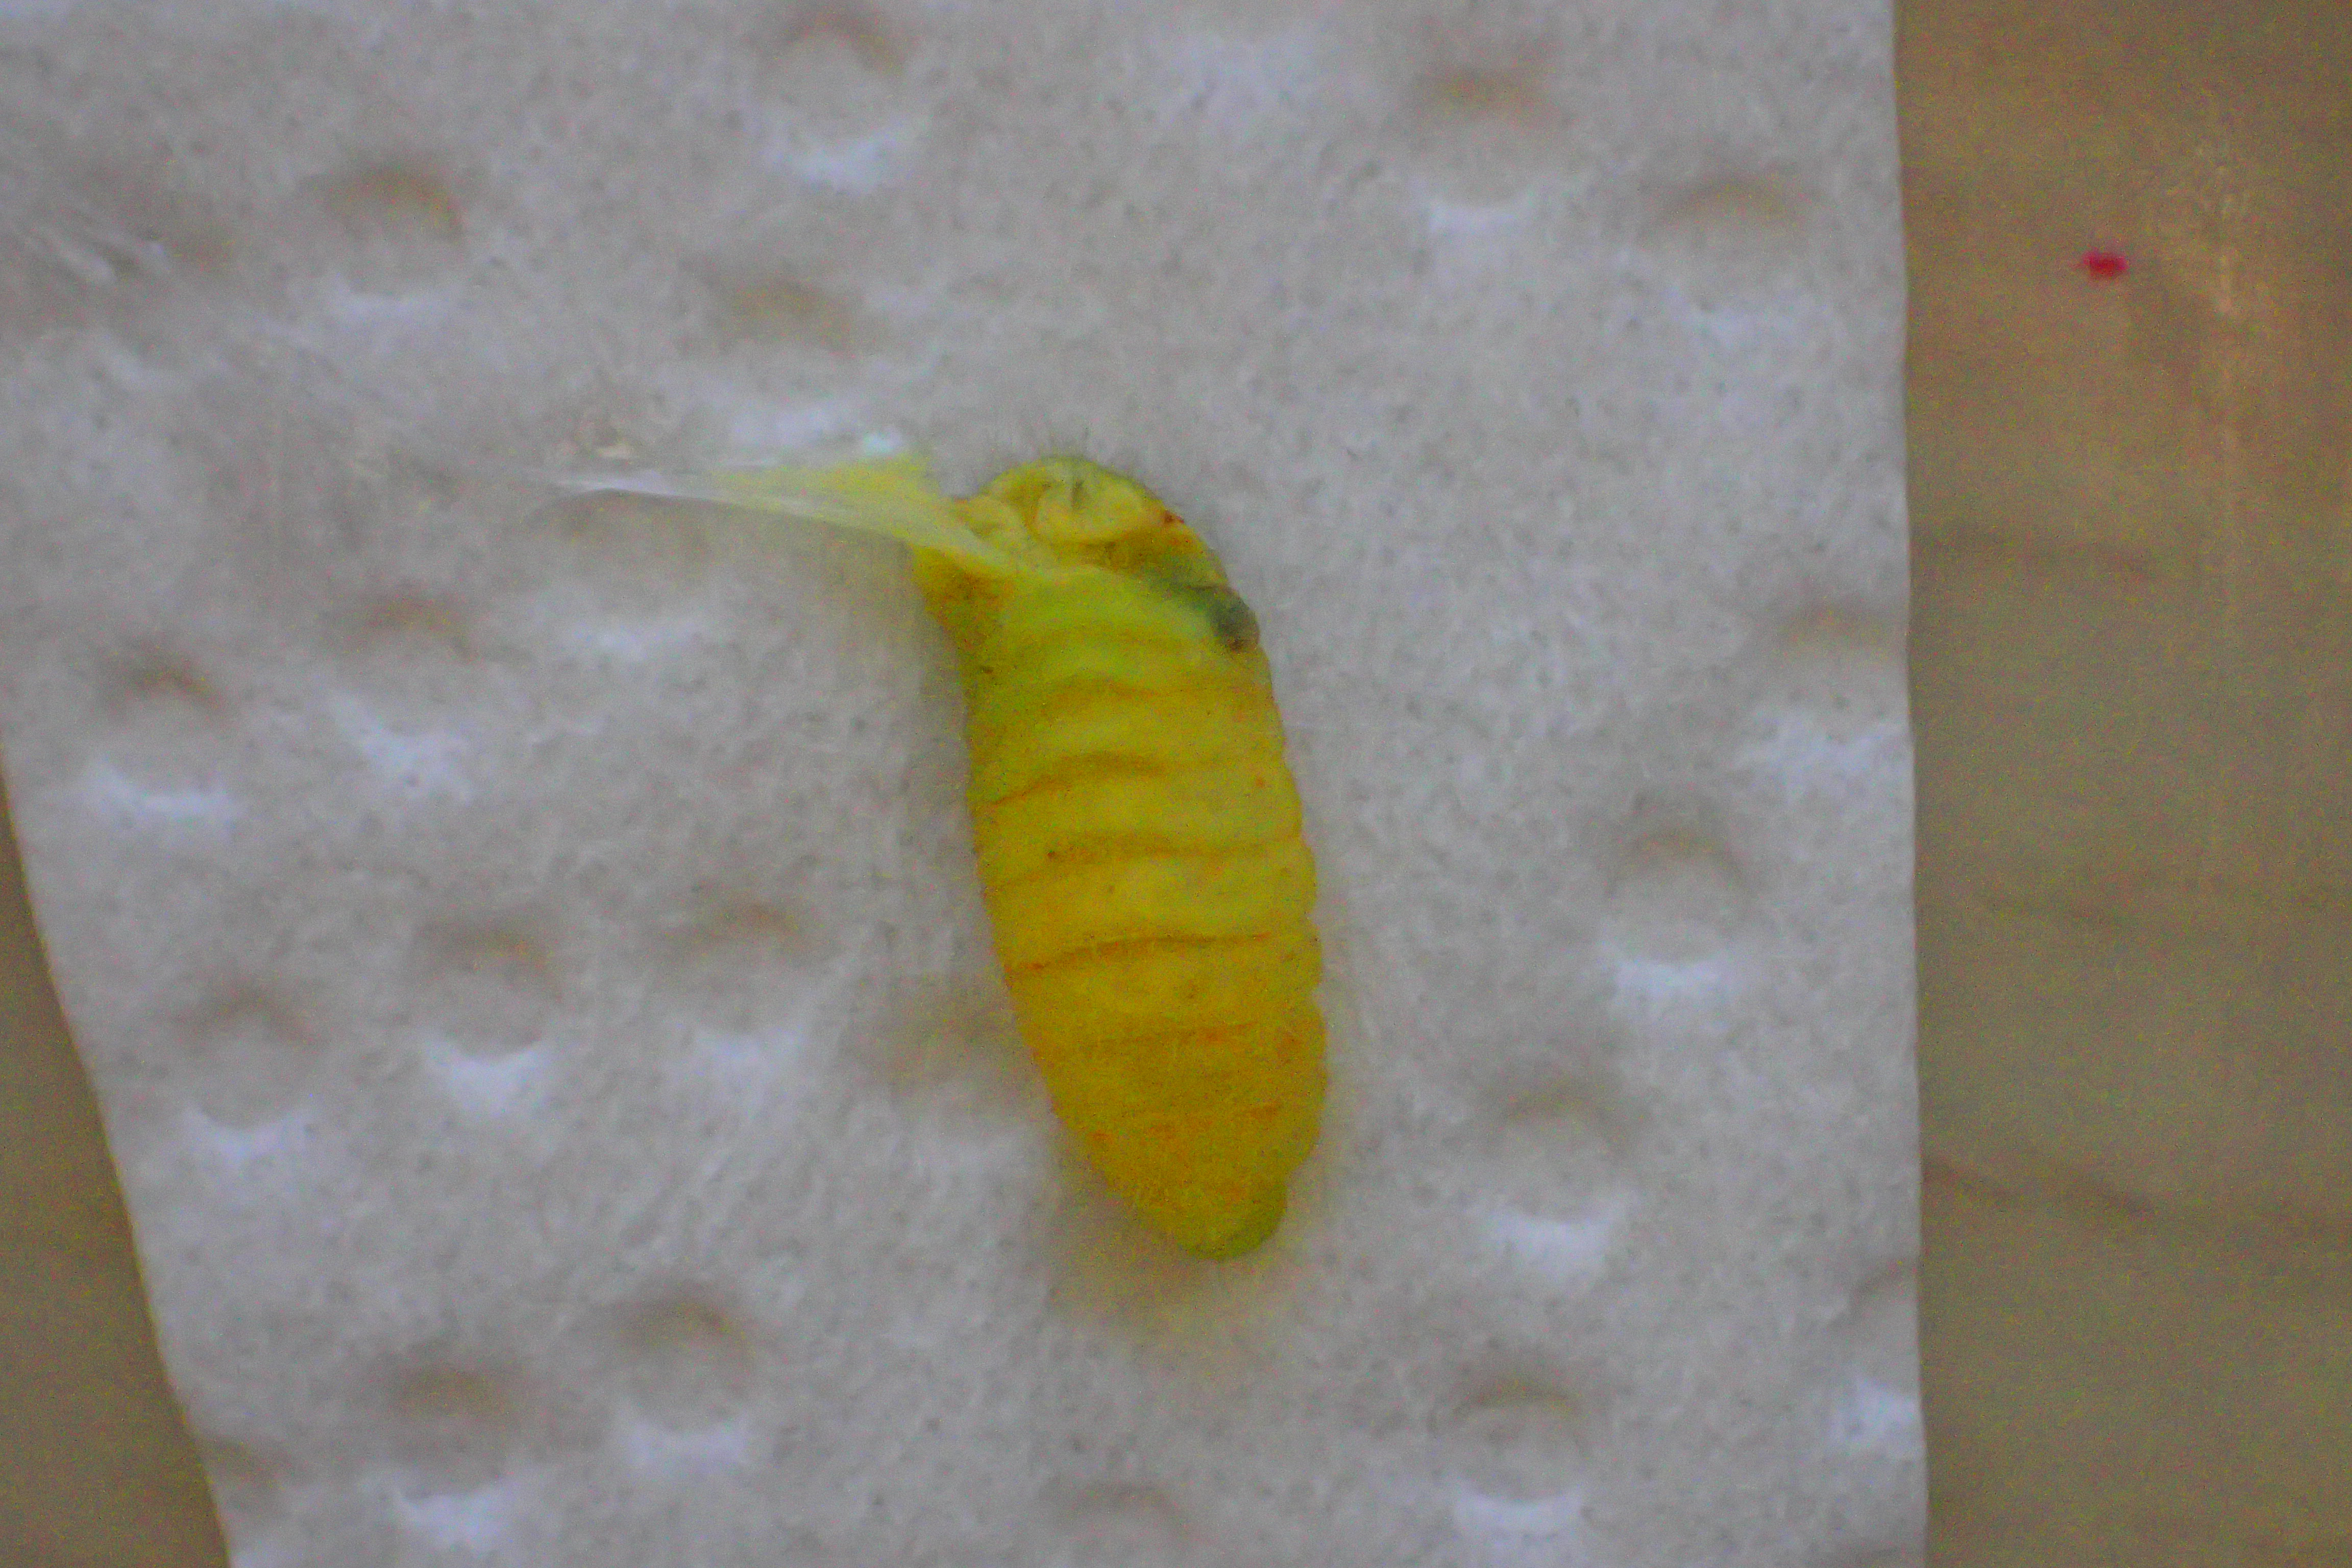
\includegraphics[width=5cm]{photo4/pupaDead.JPG}
    \end{center}
    \caption{寄生虫が出た後の蛹}
  \end{minipage}
\end{figure}

\subsection{17時:蛆虫がまだ生きている}
蛆虫の生命力の高さはしっていたが, 無酸素状態で1時間以上たっているのに, まだ水中で動いている. 
たいしたものだ. 

\subsection{22時:幼虫4が前蛹になった}
夕方より, 幼虫4が, やたらと食草を離れ, ケースの中をうろつくようになったので, 
もしかしたらと思っていたが, ガラスボウルの蓋に糸を貼り, 前蛹になった. 
今回は, 特にきになる斑点もないのと, たまたまガラスボウルに付いてくれたので, 観察がしやすく, 
体内を何かが蠢く様子もないので, おそらく成功だ. 
キッチンペーパーには, あちこちに, 水分を多量に含んだと思われる糞の痕跡があった. 
2時間程度全く動かなかったが, その後, 糸による足場の強化をし, 完全に動かなくなった. 
\begin{figure}[htbp]
  \begin{center}
    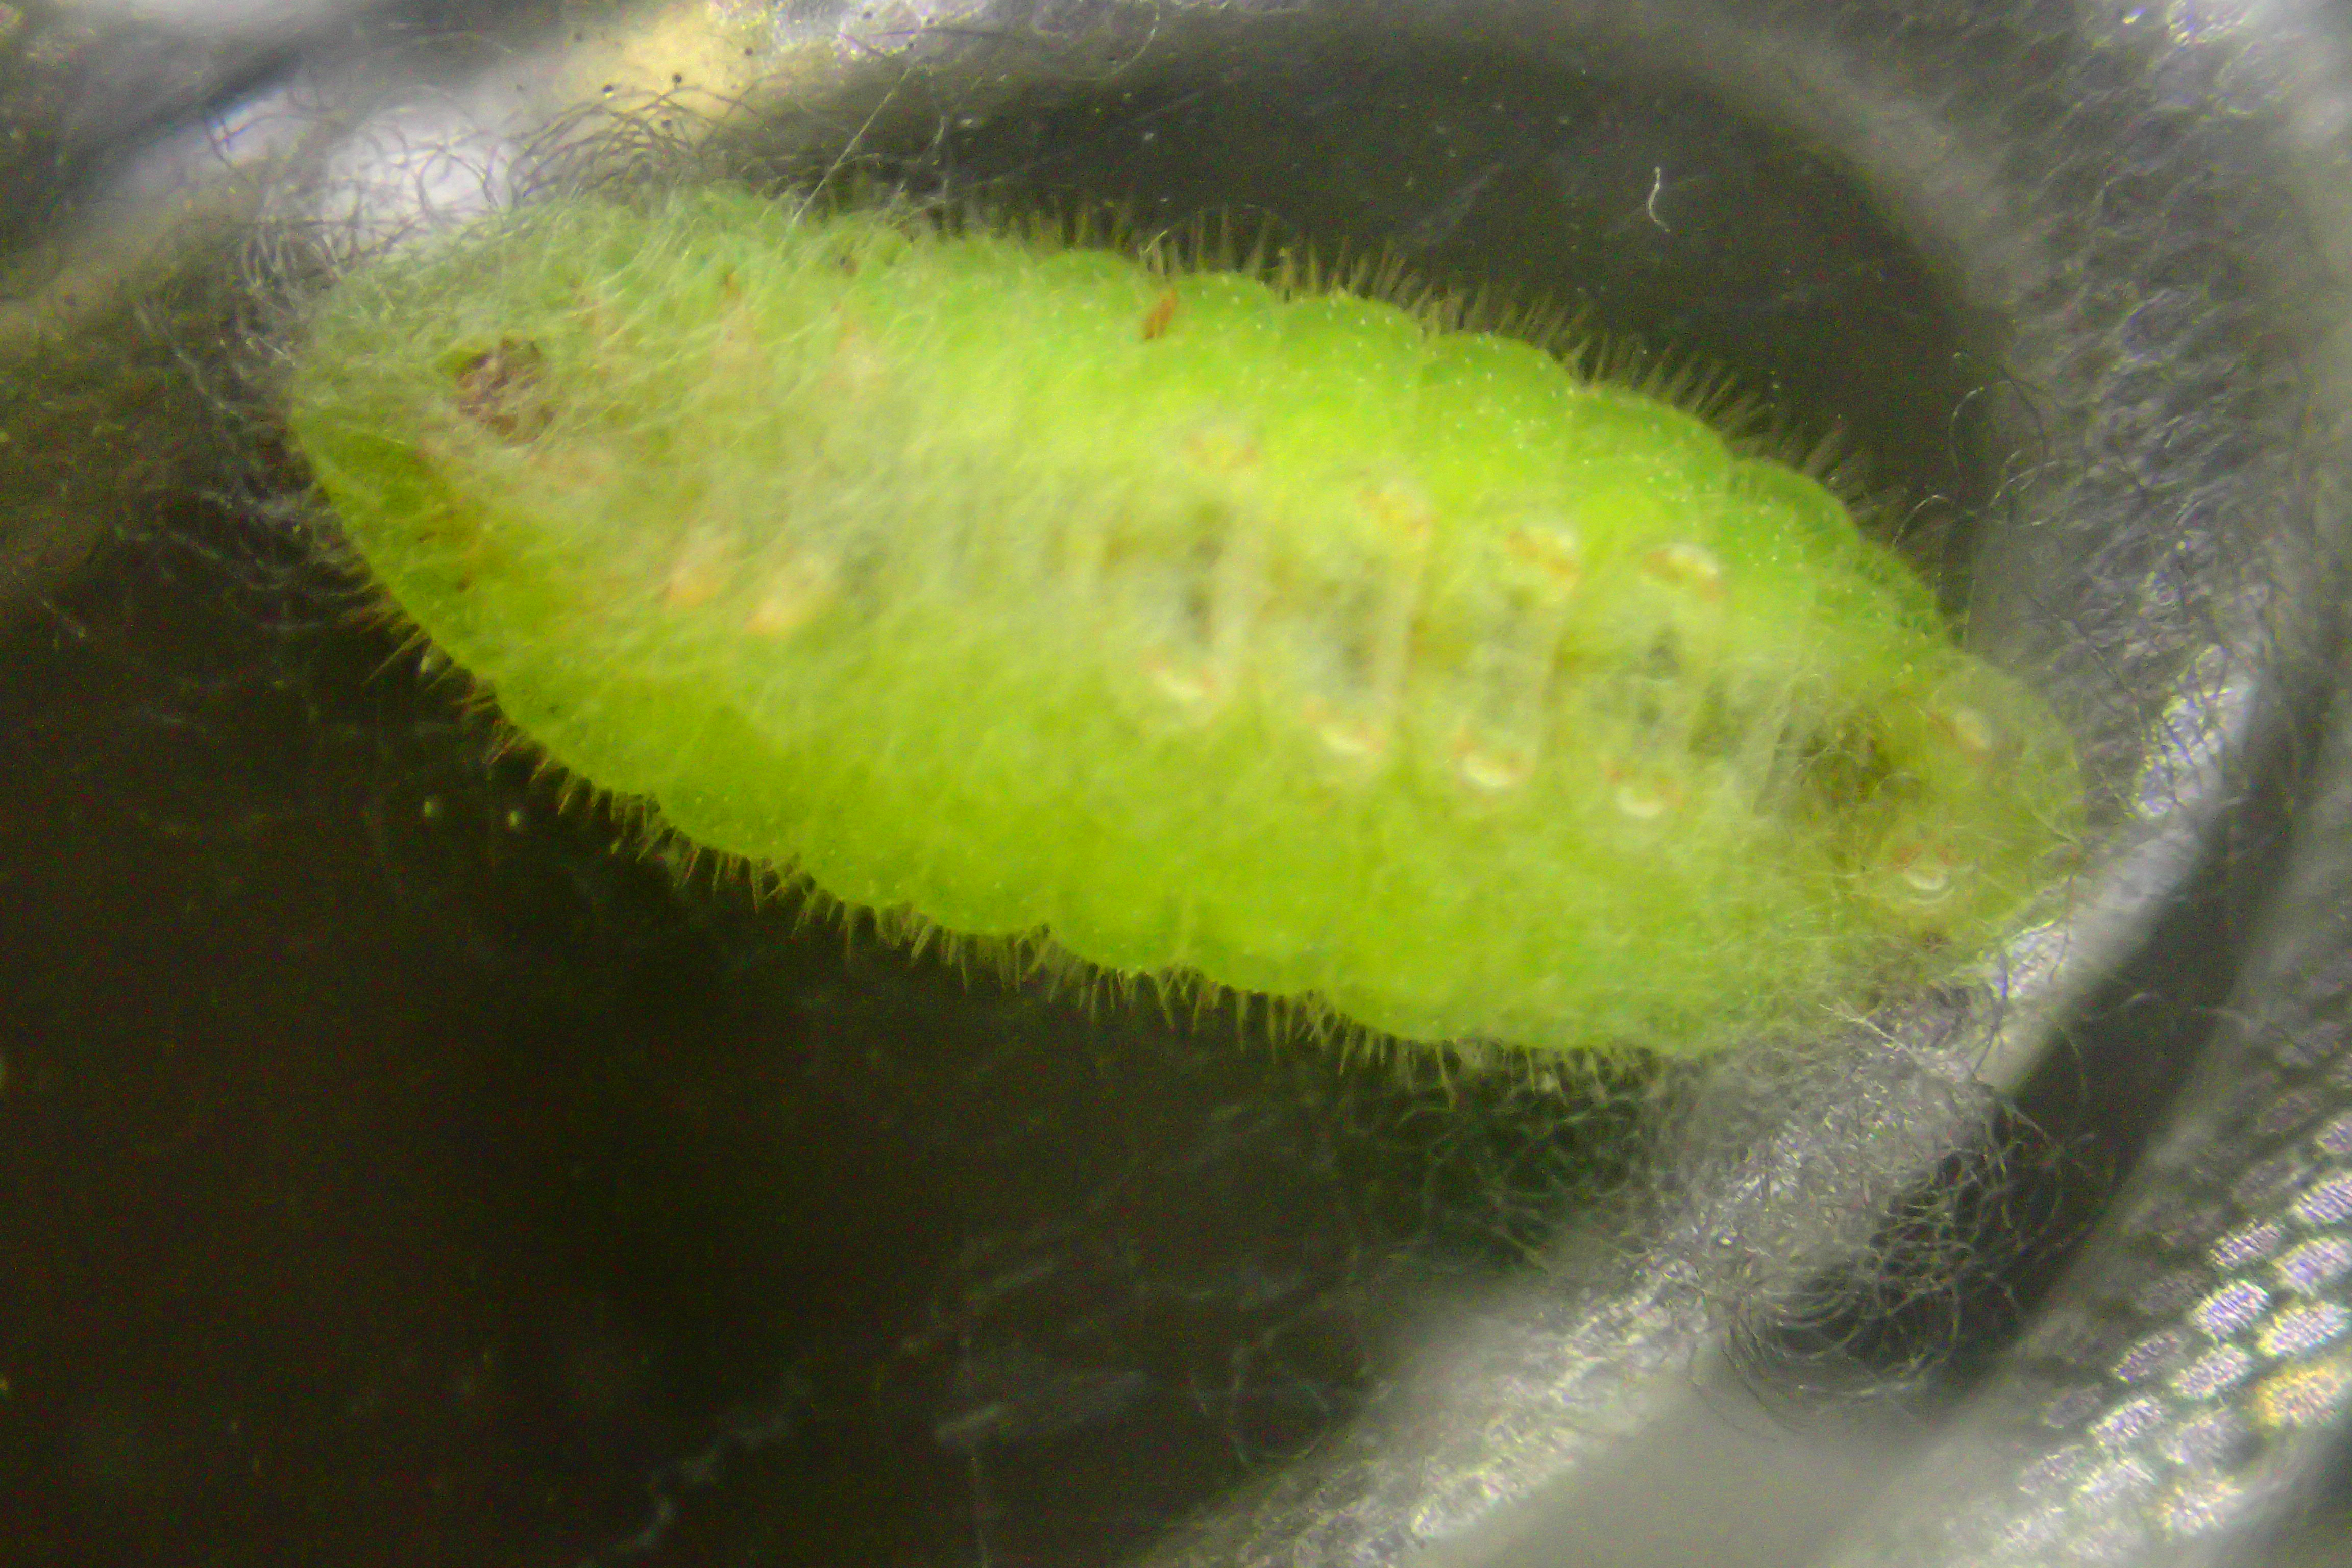
\includegraphics[width=5cm]{photo4/prePupa.JPG}
  \end{center}
  \caption{幼虫4が前蛹になった}
\end{figure}

\subsection{23時:幼虫5が前蛹になった, と思われる}
幼虫5が, 少し気になる動きをした. 先に死んだ2匹にも見られた動作だが, 
丸まったり, 伸びたり, という, もがいているようにも見える動作である. 
これは, こいつも危ないか, と思っていたが, その後動作は落ち着いたようで, ただ, キッチンペーパーの上に落ち着いていた. 
よく見ると, 頭部付近に, 細い筋が見られ, おそらく, 体を固定する糸ではないかと思われる. 
光を当てても反応しないし, 尾の方を見ると, 水分を出した糞の跡があり, うまくいっていれば, 前蛹, 
ダメであれば, 寄生中が体内でうごめき出した可能性がある. 
いずれにしろ, 明日になればわかる. 

\section{5/18の記録}
\subsection{10時:前蛹ではなかった}
昨日, もう一匹が前蛹になったと思っていたが, 今朝見ると普通に葉の上にいた. 
多分ただの休眠期間であったのだろう. まぎらわしい. 
最初の前蛹は, 明らかに蛹に形状が変わってきており, 今晩にでも変化するのではないだろうか. 

\subsection{15時:異常なし}
幼虫4の前蛹は, まだ幼虫の形をしているが, 前の寄生されていたやつのように, 変色したり, 染みが出てきたりはしておらず, おそらくもう少し時間がかかるのか. 
幼虫5も, 葉に張り付いてはいるものの活動がほとんどなく, 蛹化もまもなくだろう. 

\subsection{22時:異常なし}
幼虫4の前蛹は, まだ変化がない. 幼虫5は, やはり食草から離れ, いろいろなところを動き回っている. 前蛹も近い. 
一点気になるとすると, 幼虫5の頭部に近い側にある, 筋である. なんでもなければよいが. 

\begin{figure}[htbp]
  \begin{center}
    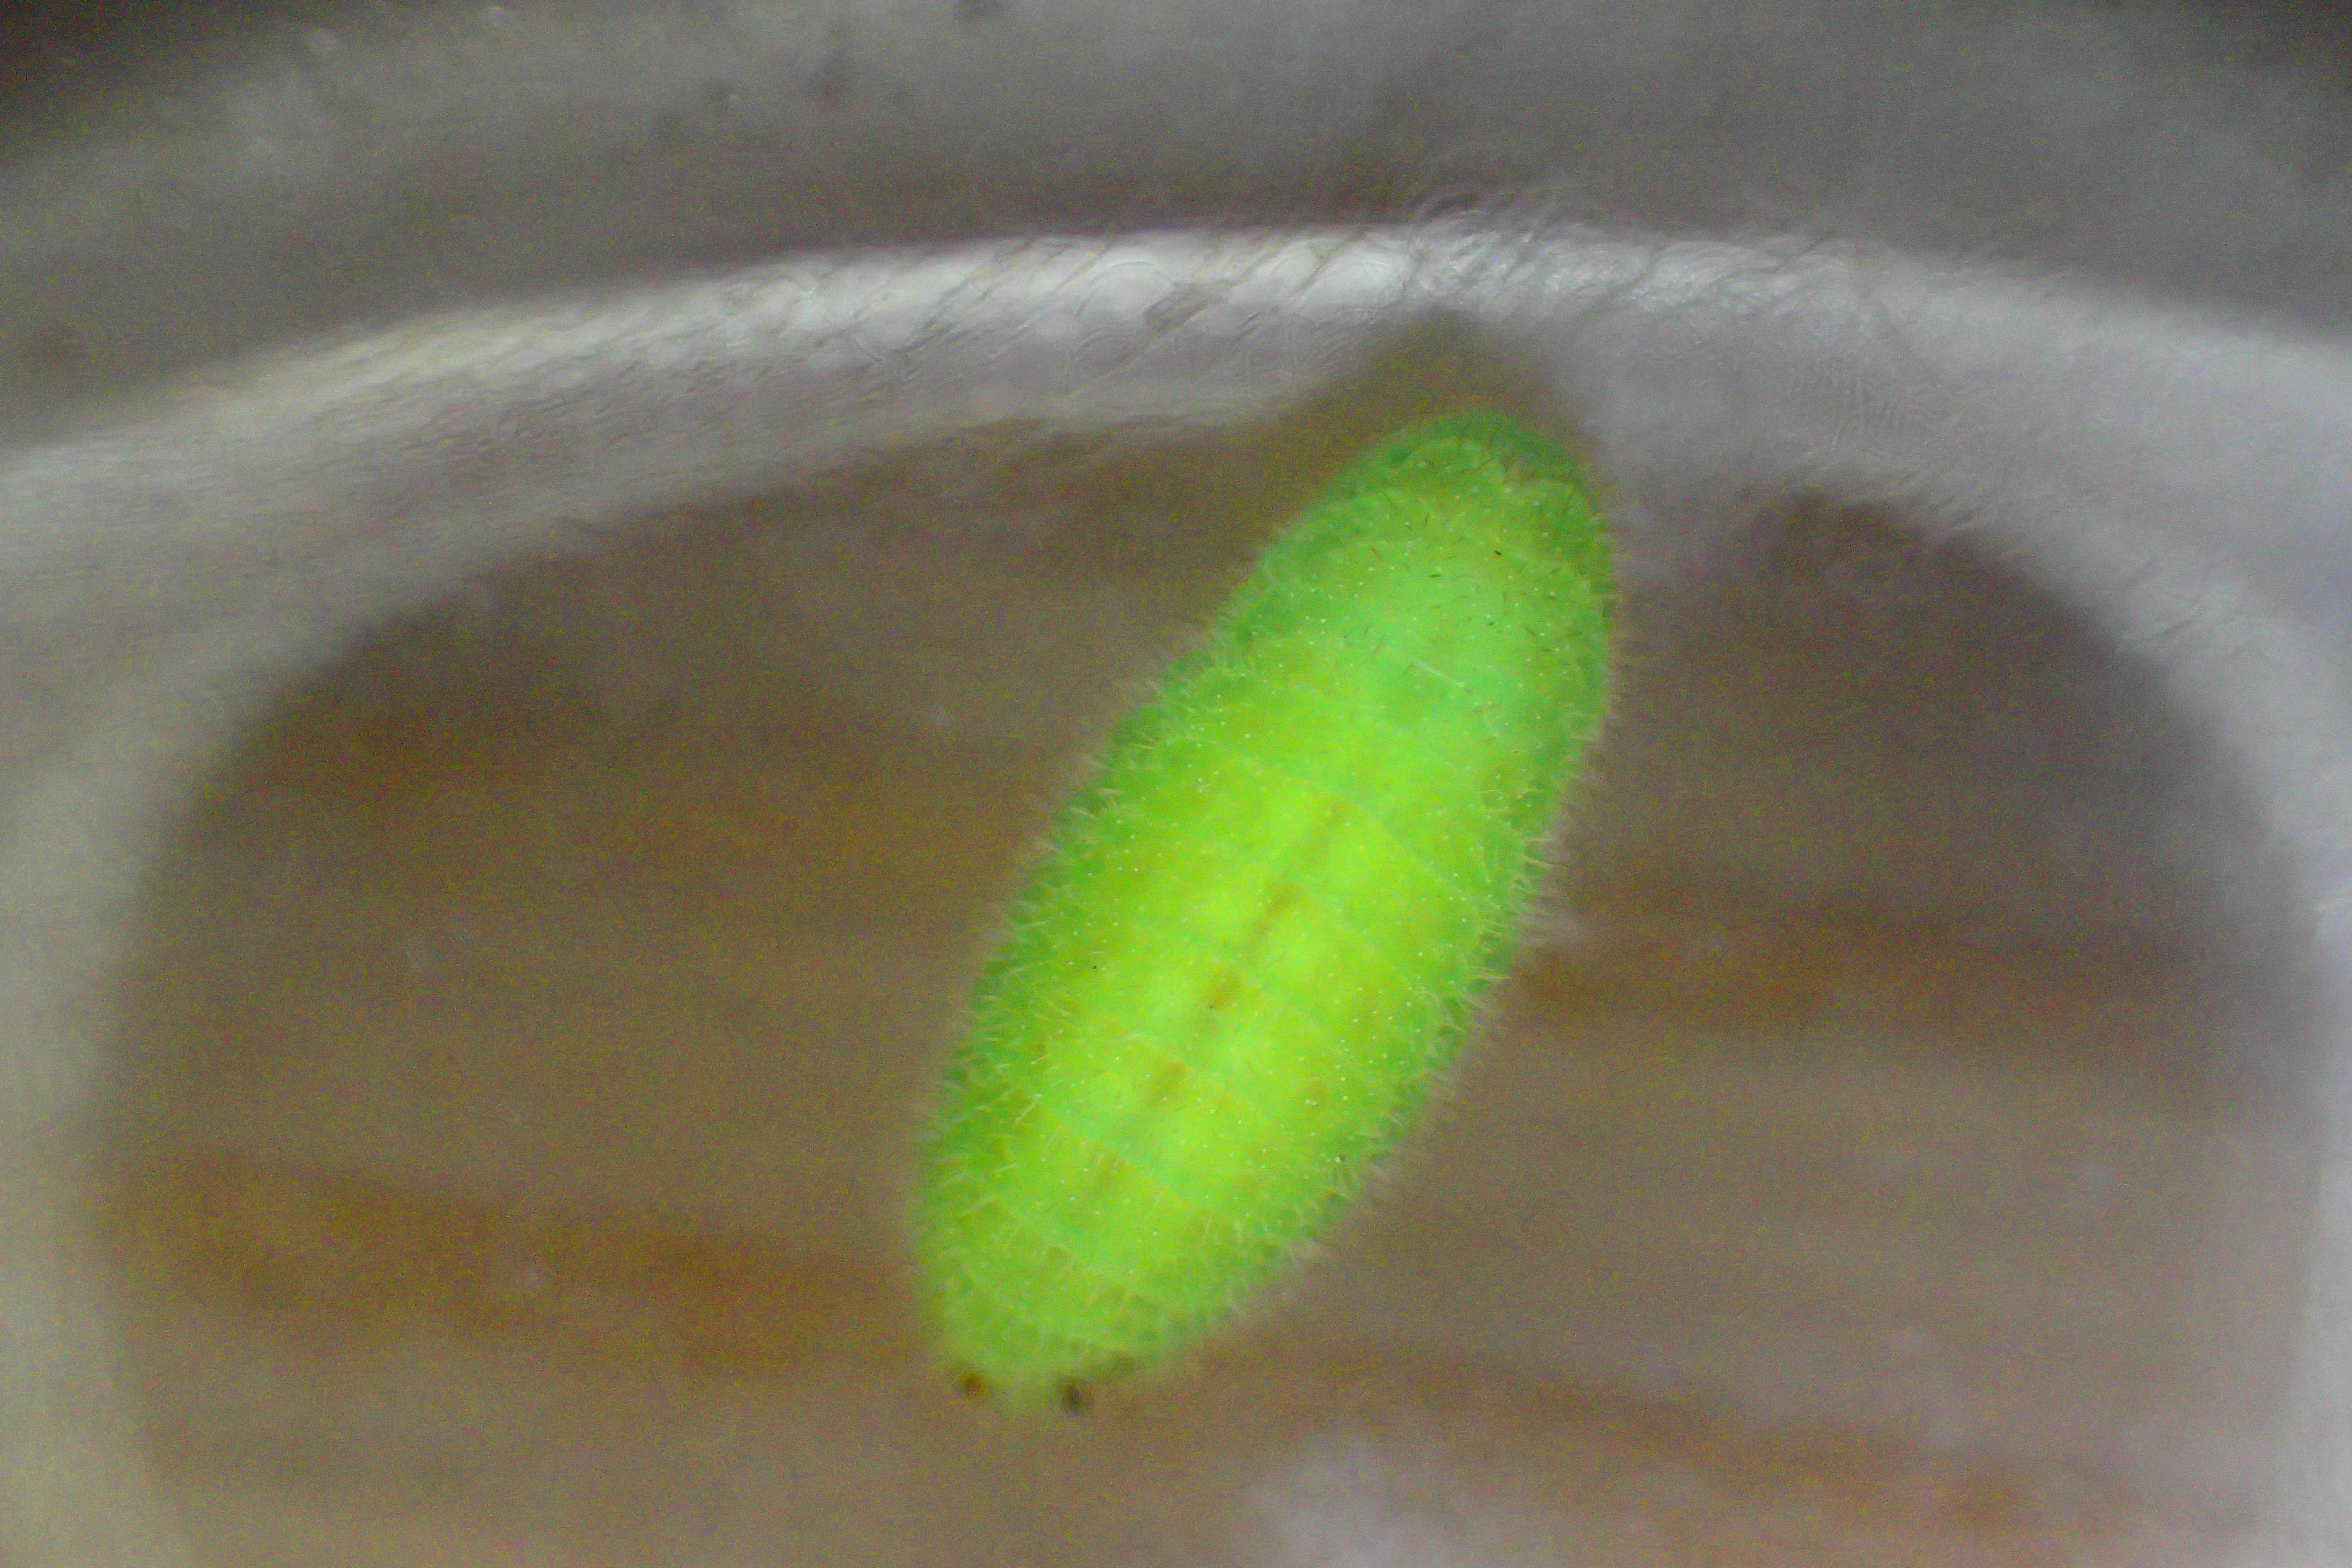
\includegraphics[width=5cm]{photo5/Larva4-prePupa.JPG}
  \end{center}
  \caption{幼虫4の前蛹はまだ変化なし}
\end{figure}

\begin{figure}[htbp]
  \begin{center}
    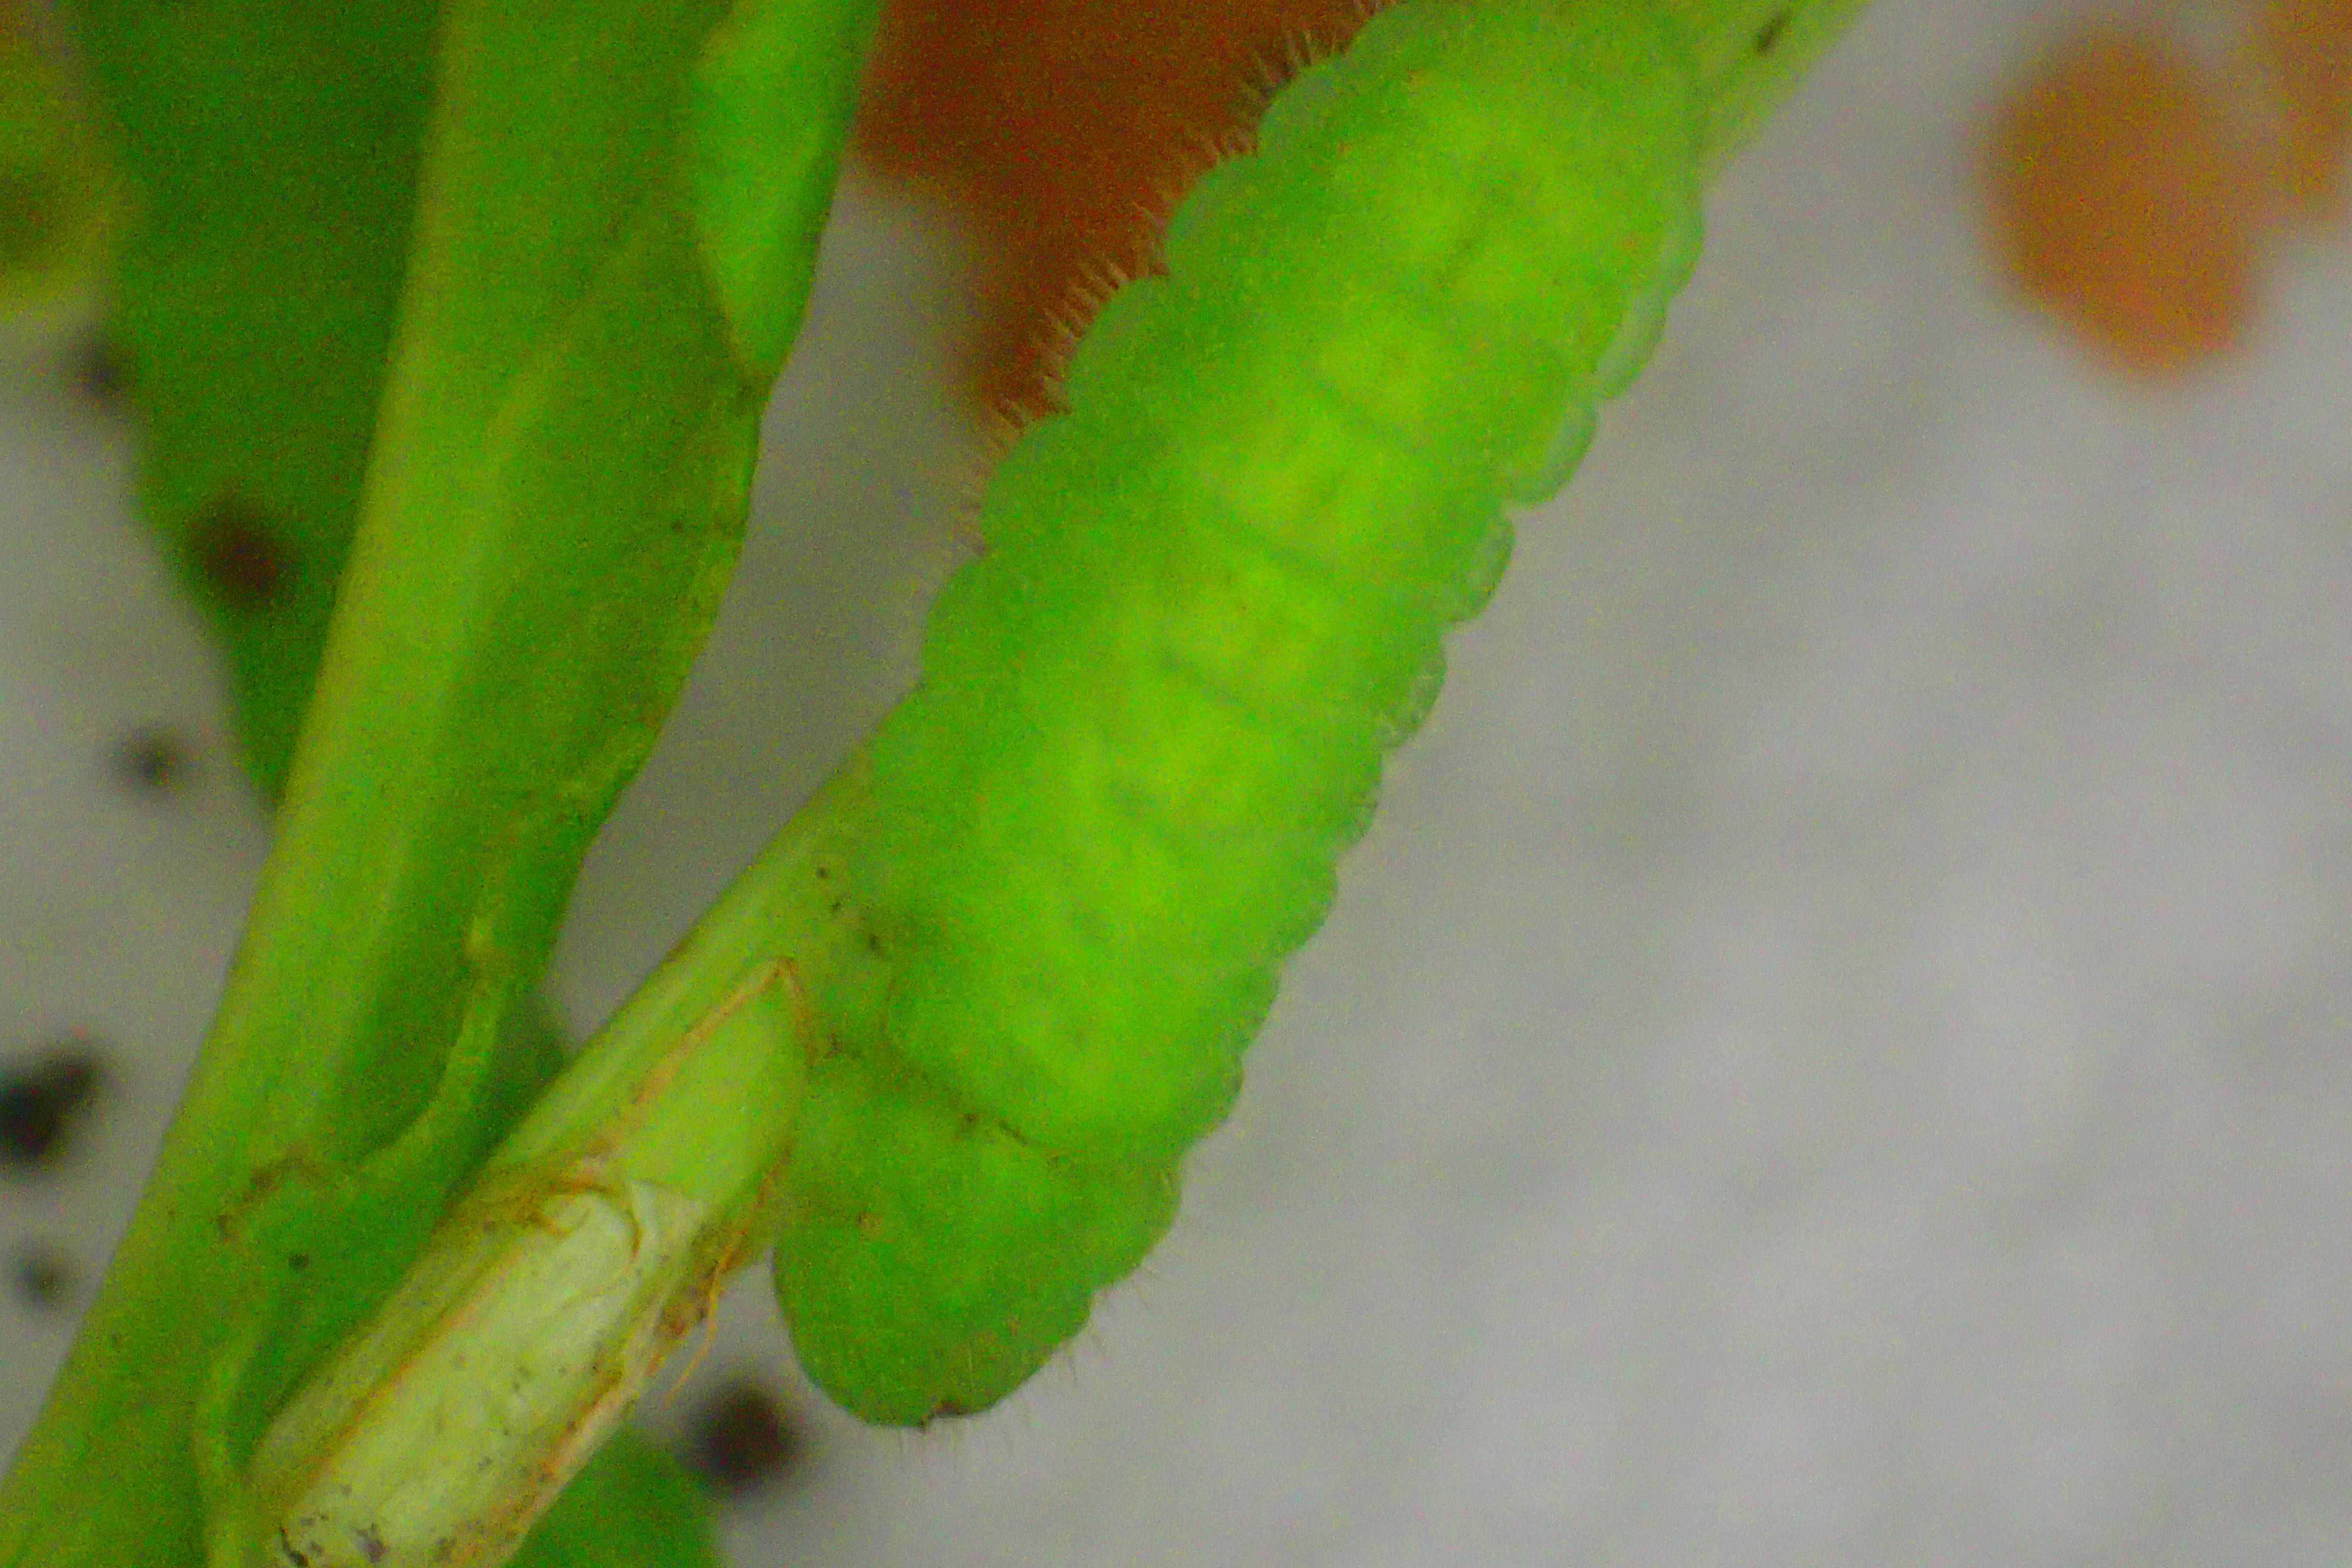
\includegraphics[width=5cm]{photo5/Larva5.JPG}
  \end{center}
  \caption{幼虫5の頭部に近い方に筋がある}
\end{figure}

\section{5/19の記録}
\subsection{10時:幼虫4が蛹化した}
起きて見ると, 幼虫4が蛹化していた. 脱ぎ捨てた皮が, 下に落ちていた. とりあえず無事成功. 
幼虫5, 6はあいかわらずである. 

\begin{figure}[htbp]
  \begin{center}
    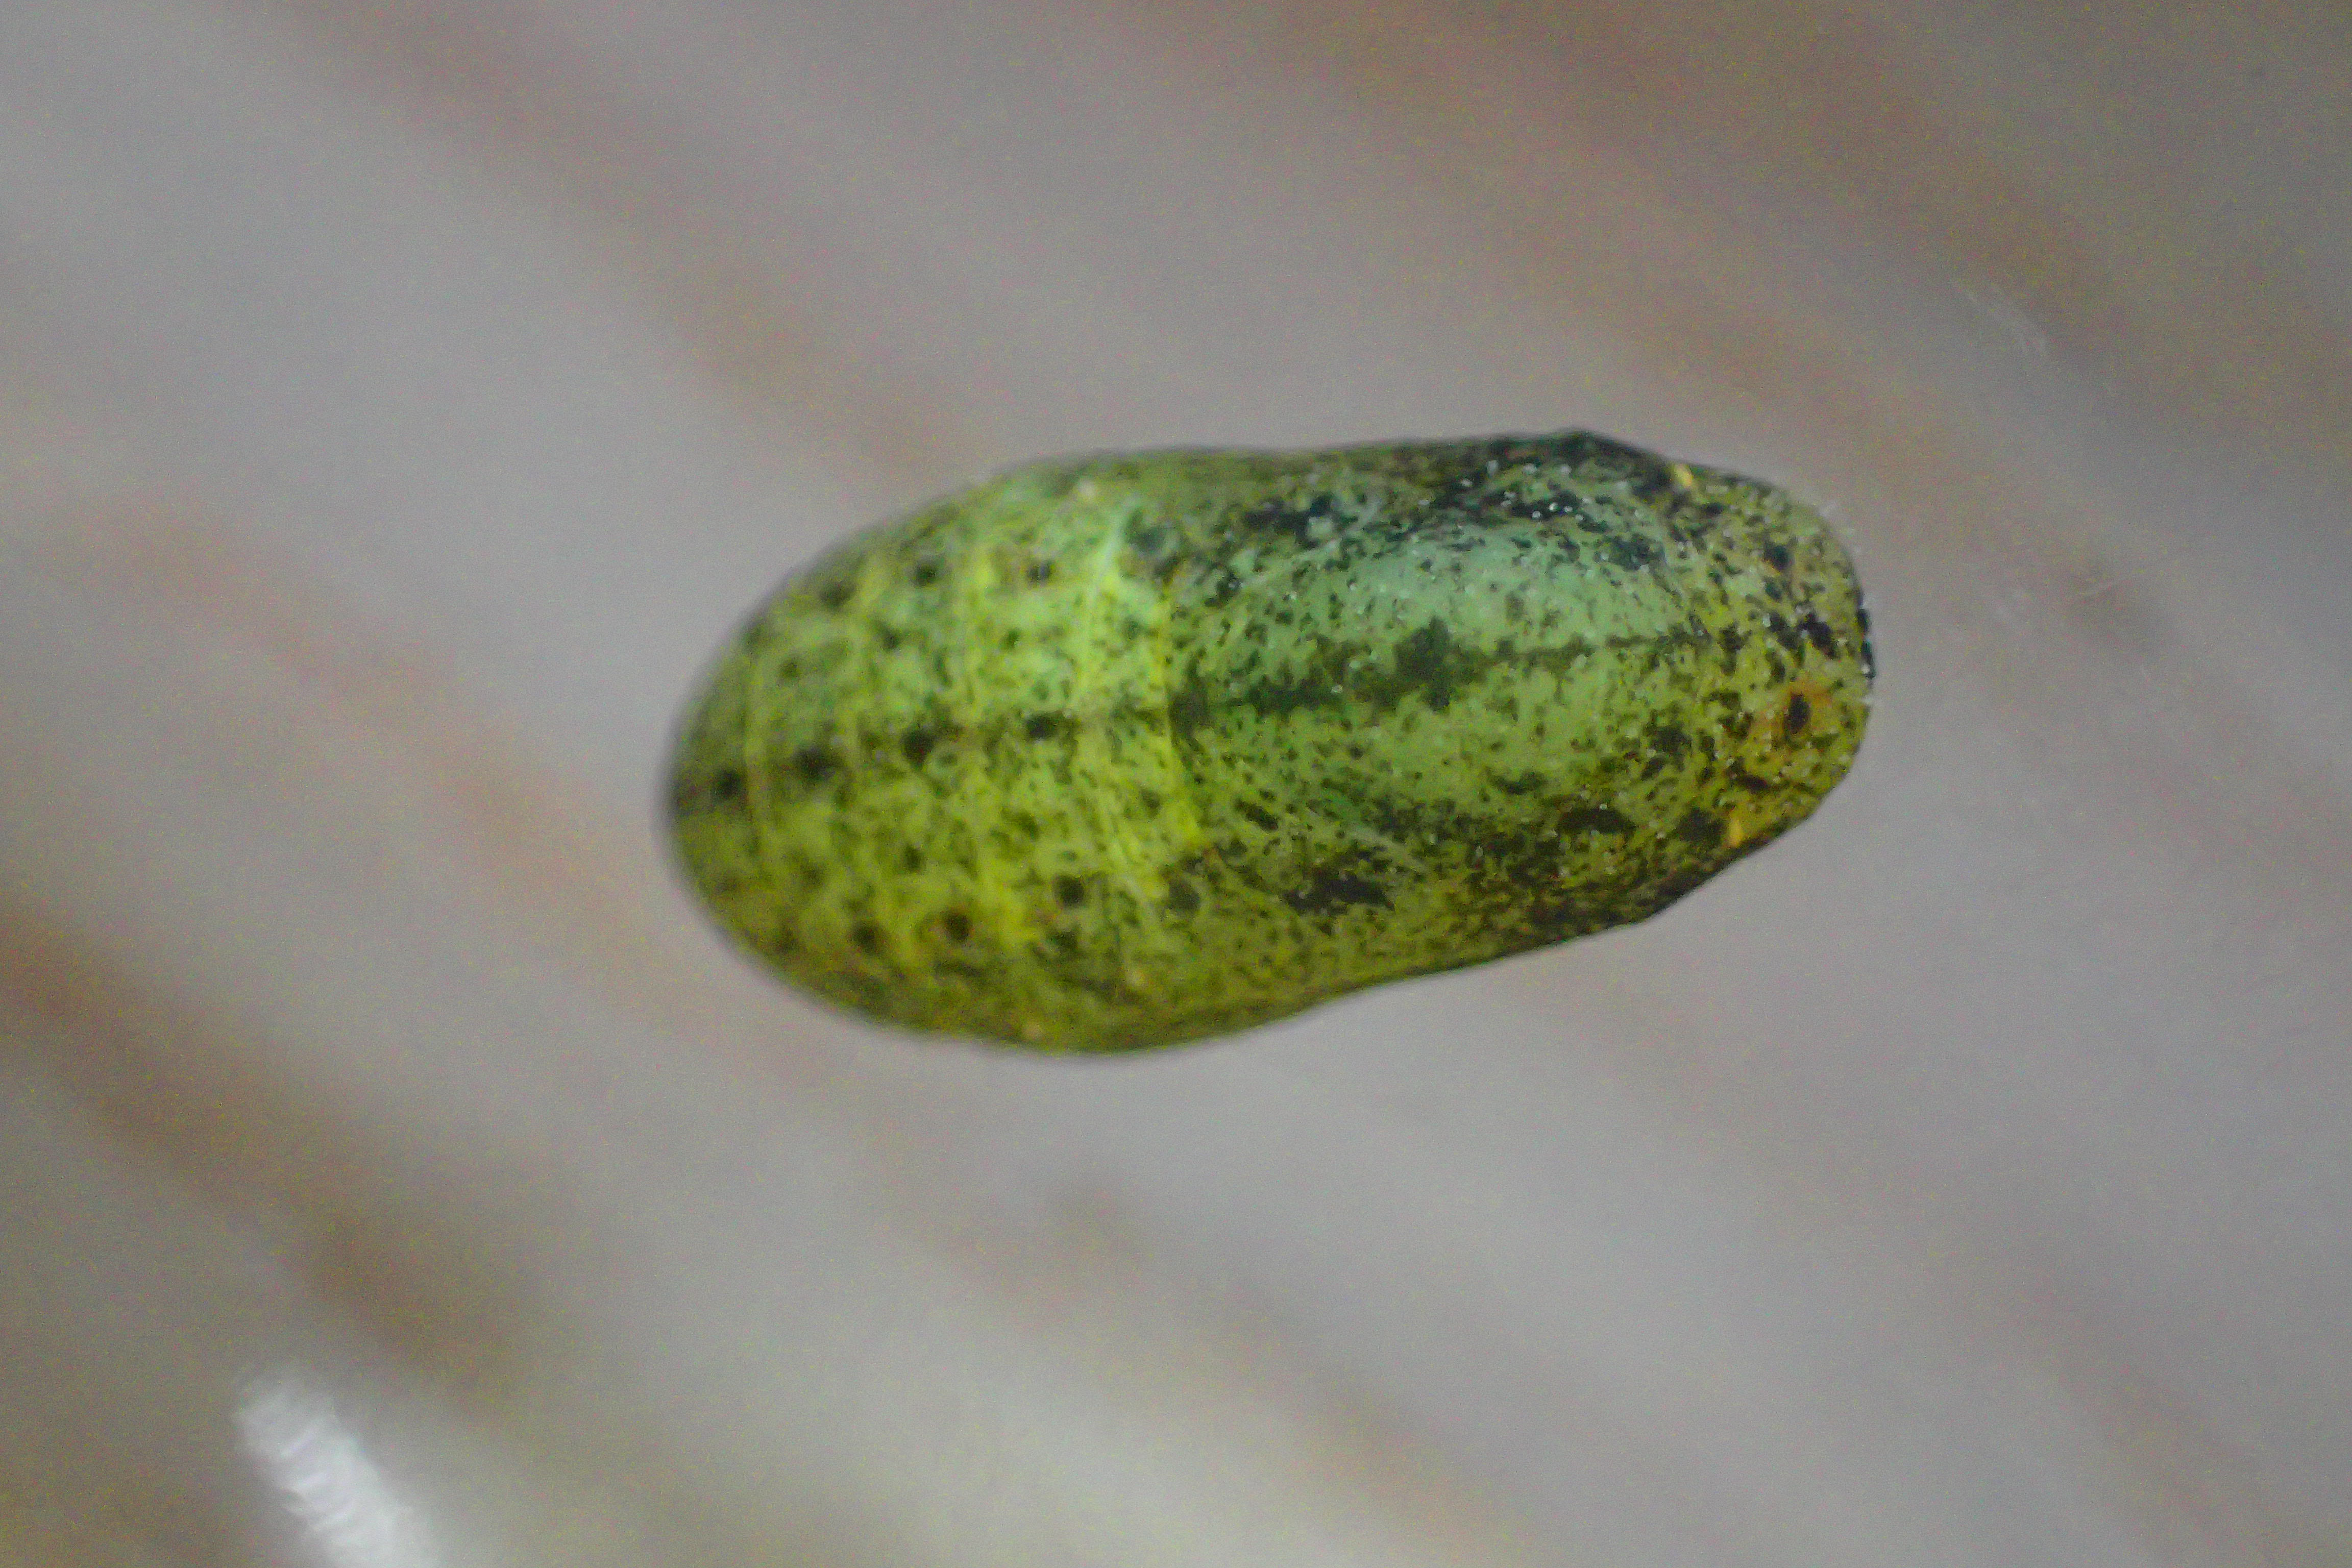
\includegraphics[width=5cm]{photo6/Larva4-pupa1.JPG}
  \end{center}
  \caption{幼虫4の蛹}
\end{figure}

\begin{figure}[htbp]
  \begin{center}
    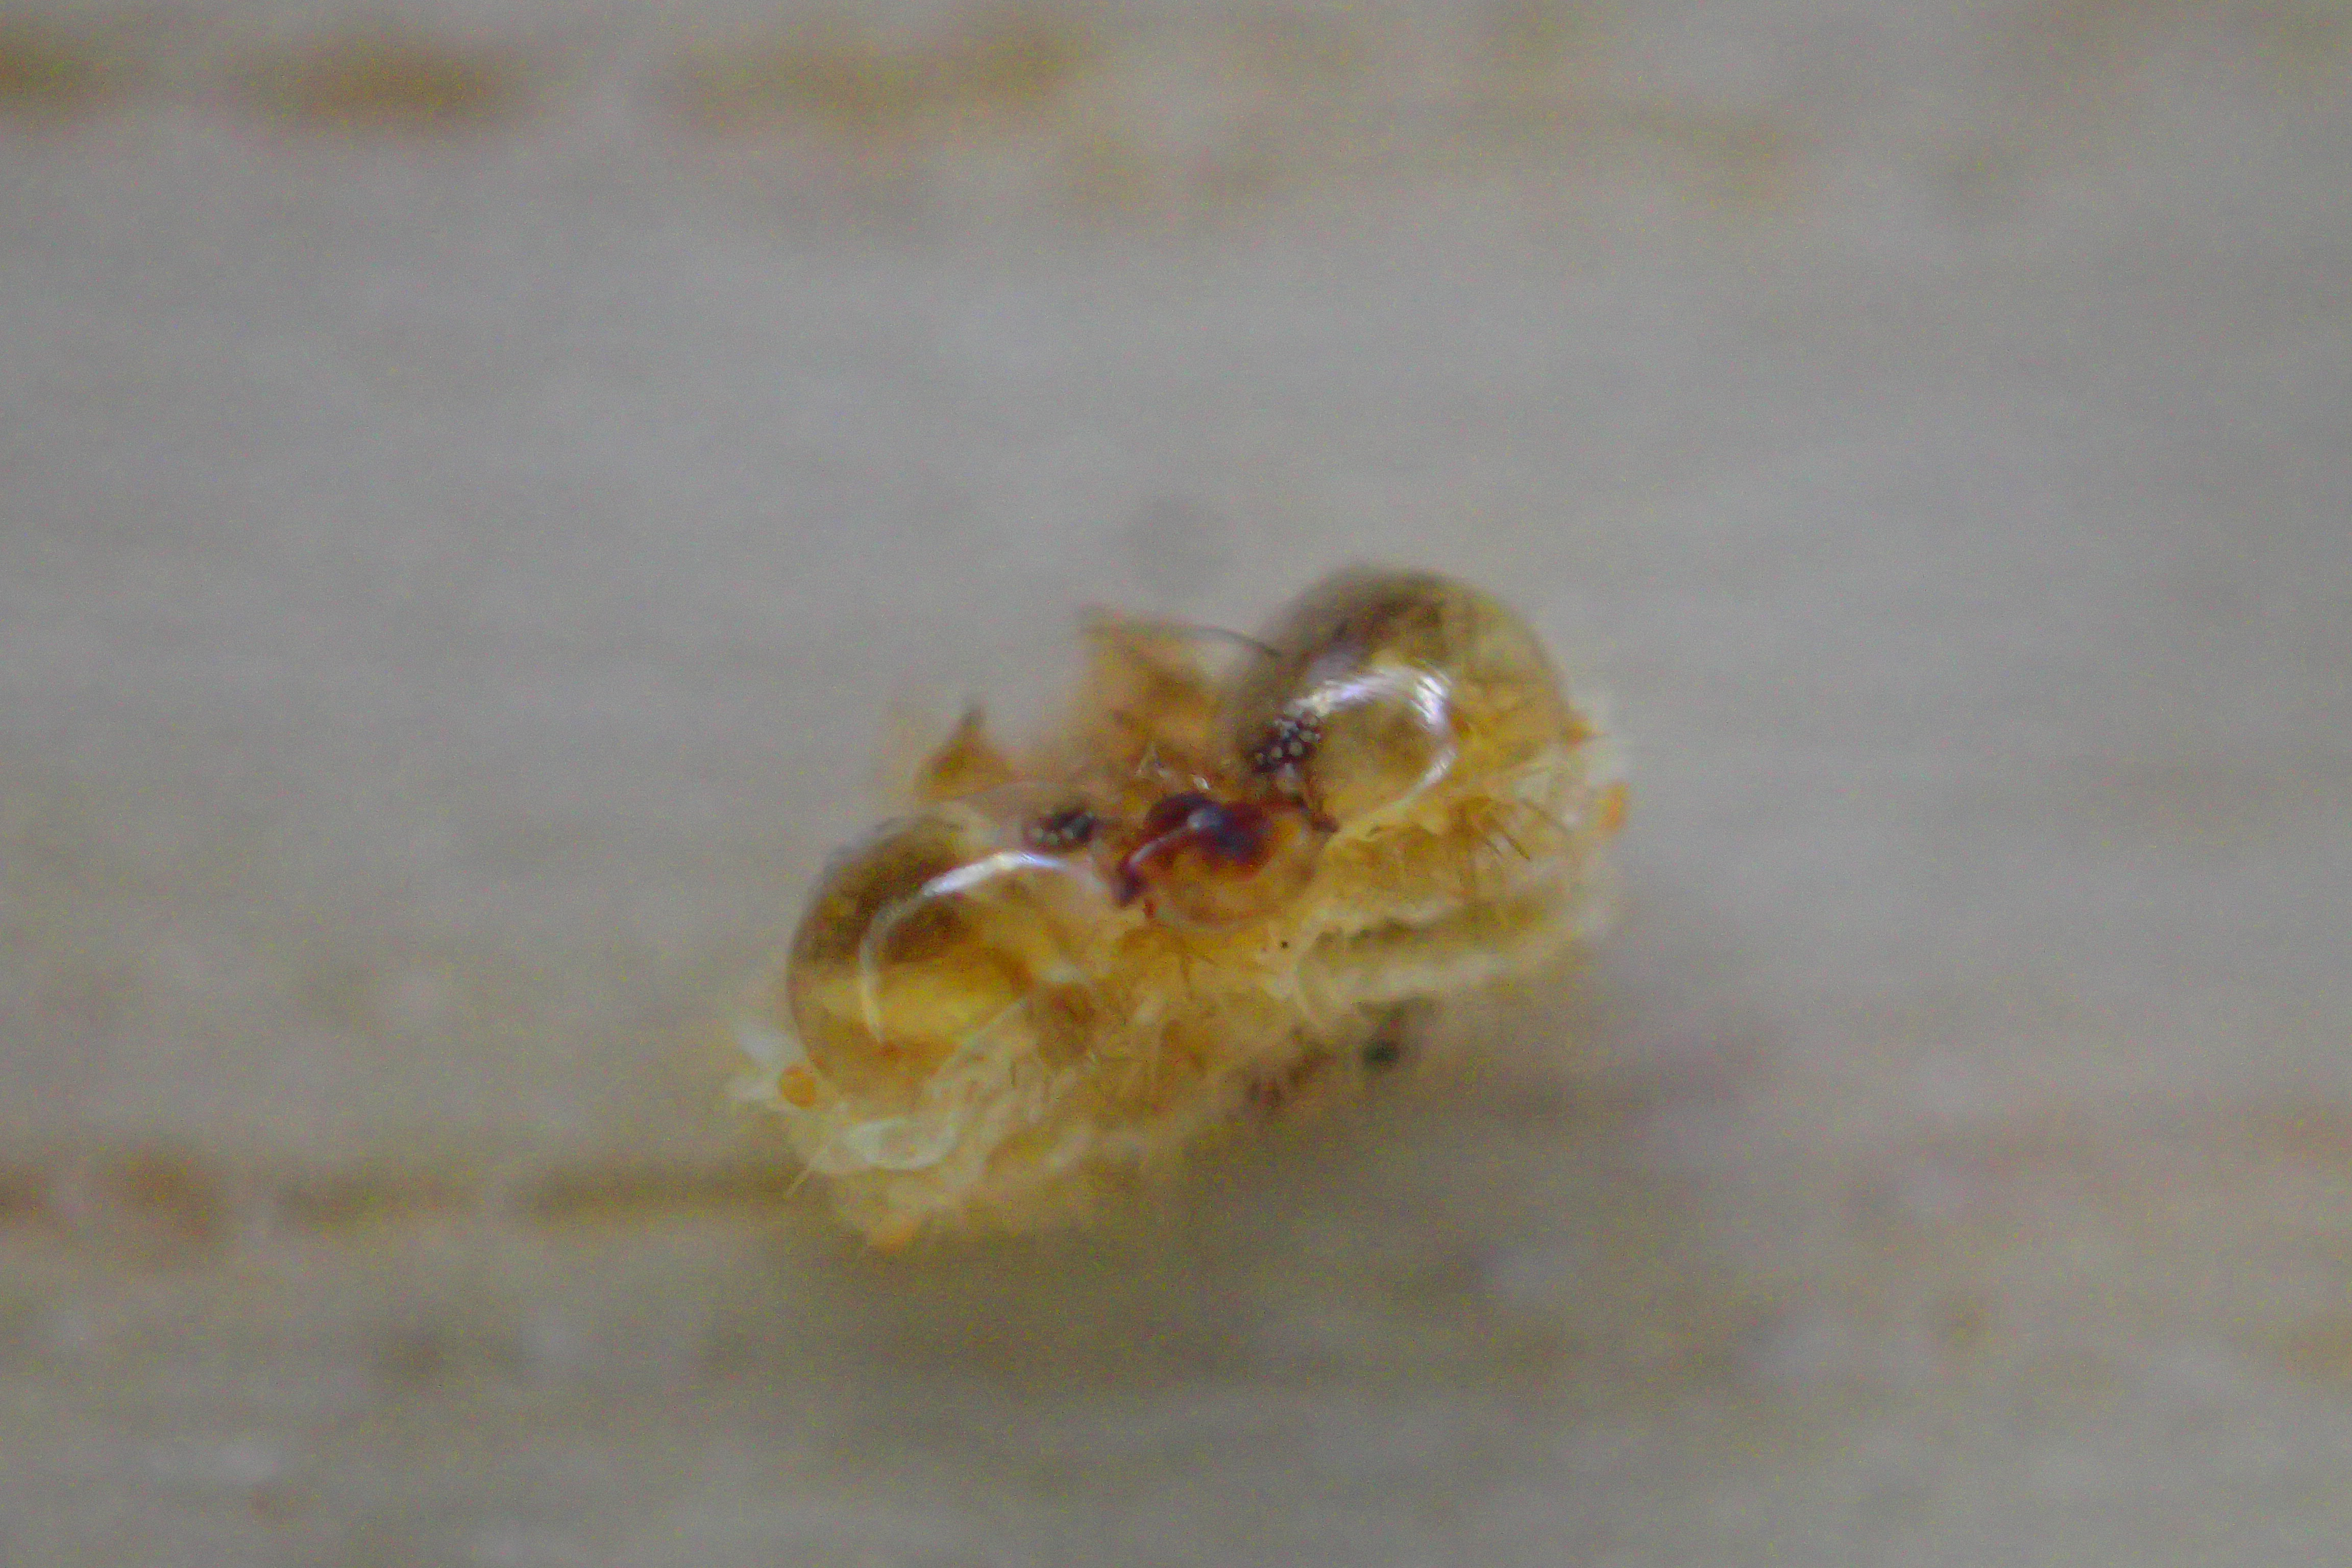
\includegraphics[width=5cm]{photo6/Larva4-oldSkin.JPG}
  \end{center}
  \caption{幼虫4の脱皮}
\end{figure}

\subsection{14時:異常なし}
幼虫4の蛹は, 心なしか, 朝よりも色味が黒い部分が多くなり, 蛹らしい見た目に変化しているように見える. 
幼虫5は, 餌から離れ, キッチンペーパーの上で静止しているが, 体勢的に, まだ前蛹ではなく, 休眠中であろう. 
幼虫6も, 餌からな離れ, キッチンペーパーの上で静止している. こちらも休眠か. 
幼虫4のようにガラスボウルで蛹になられるのも管理上微妙なので, 落ち葉に見立てて, 画用紙を切ったものをいれてやった. 

\begin{figure}[htbp]
  \begin{center}
    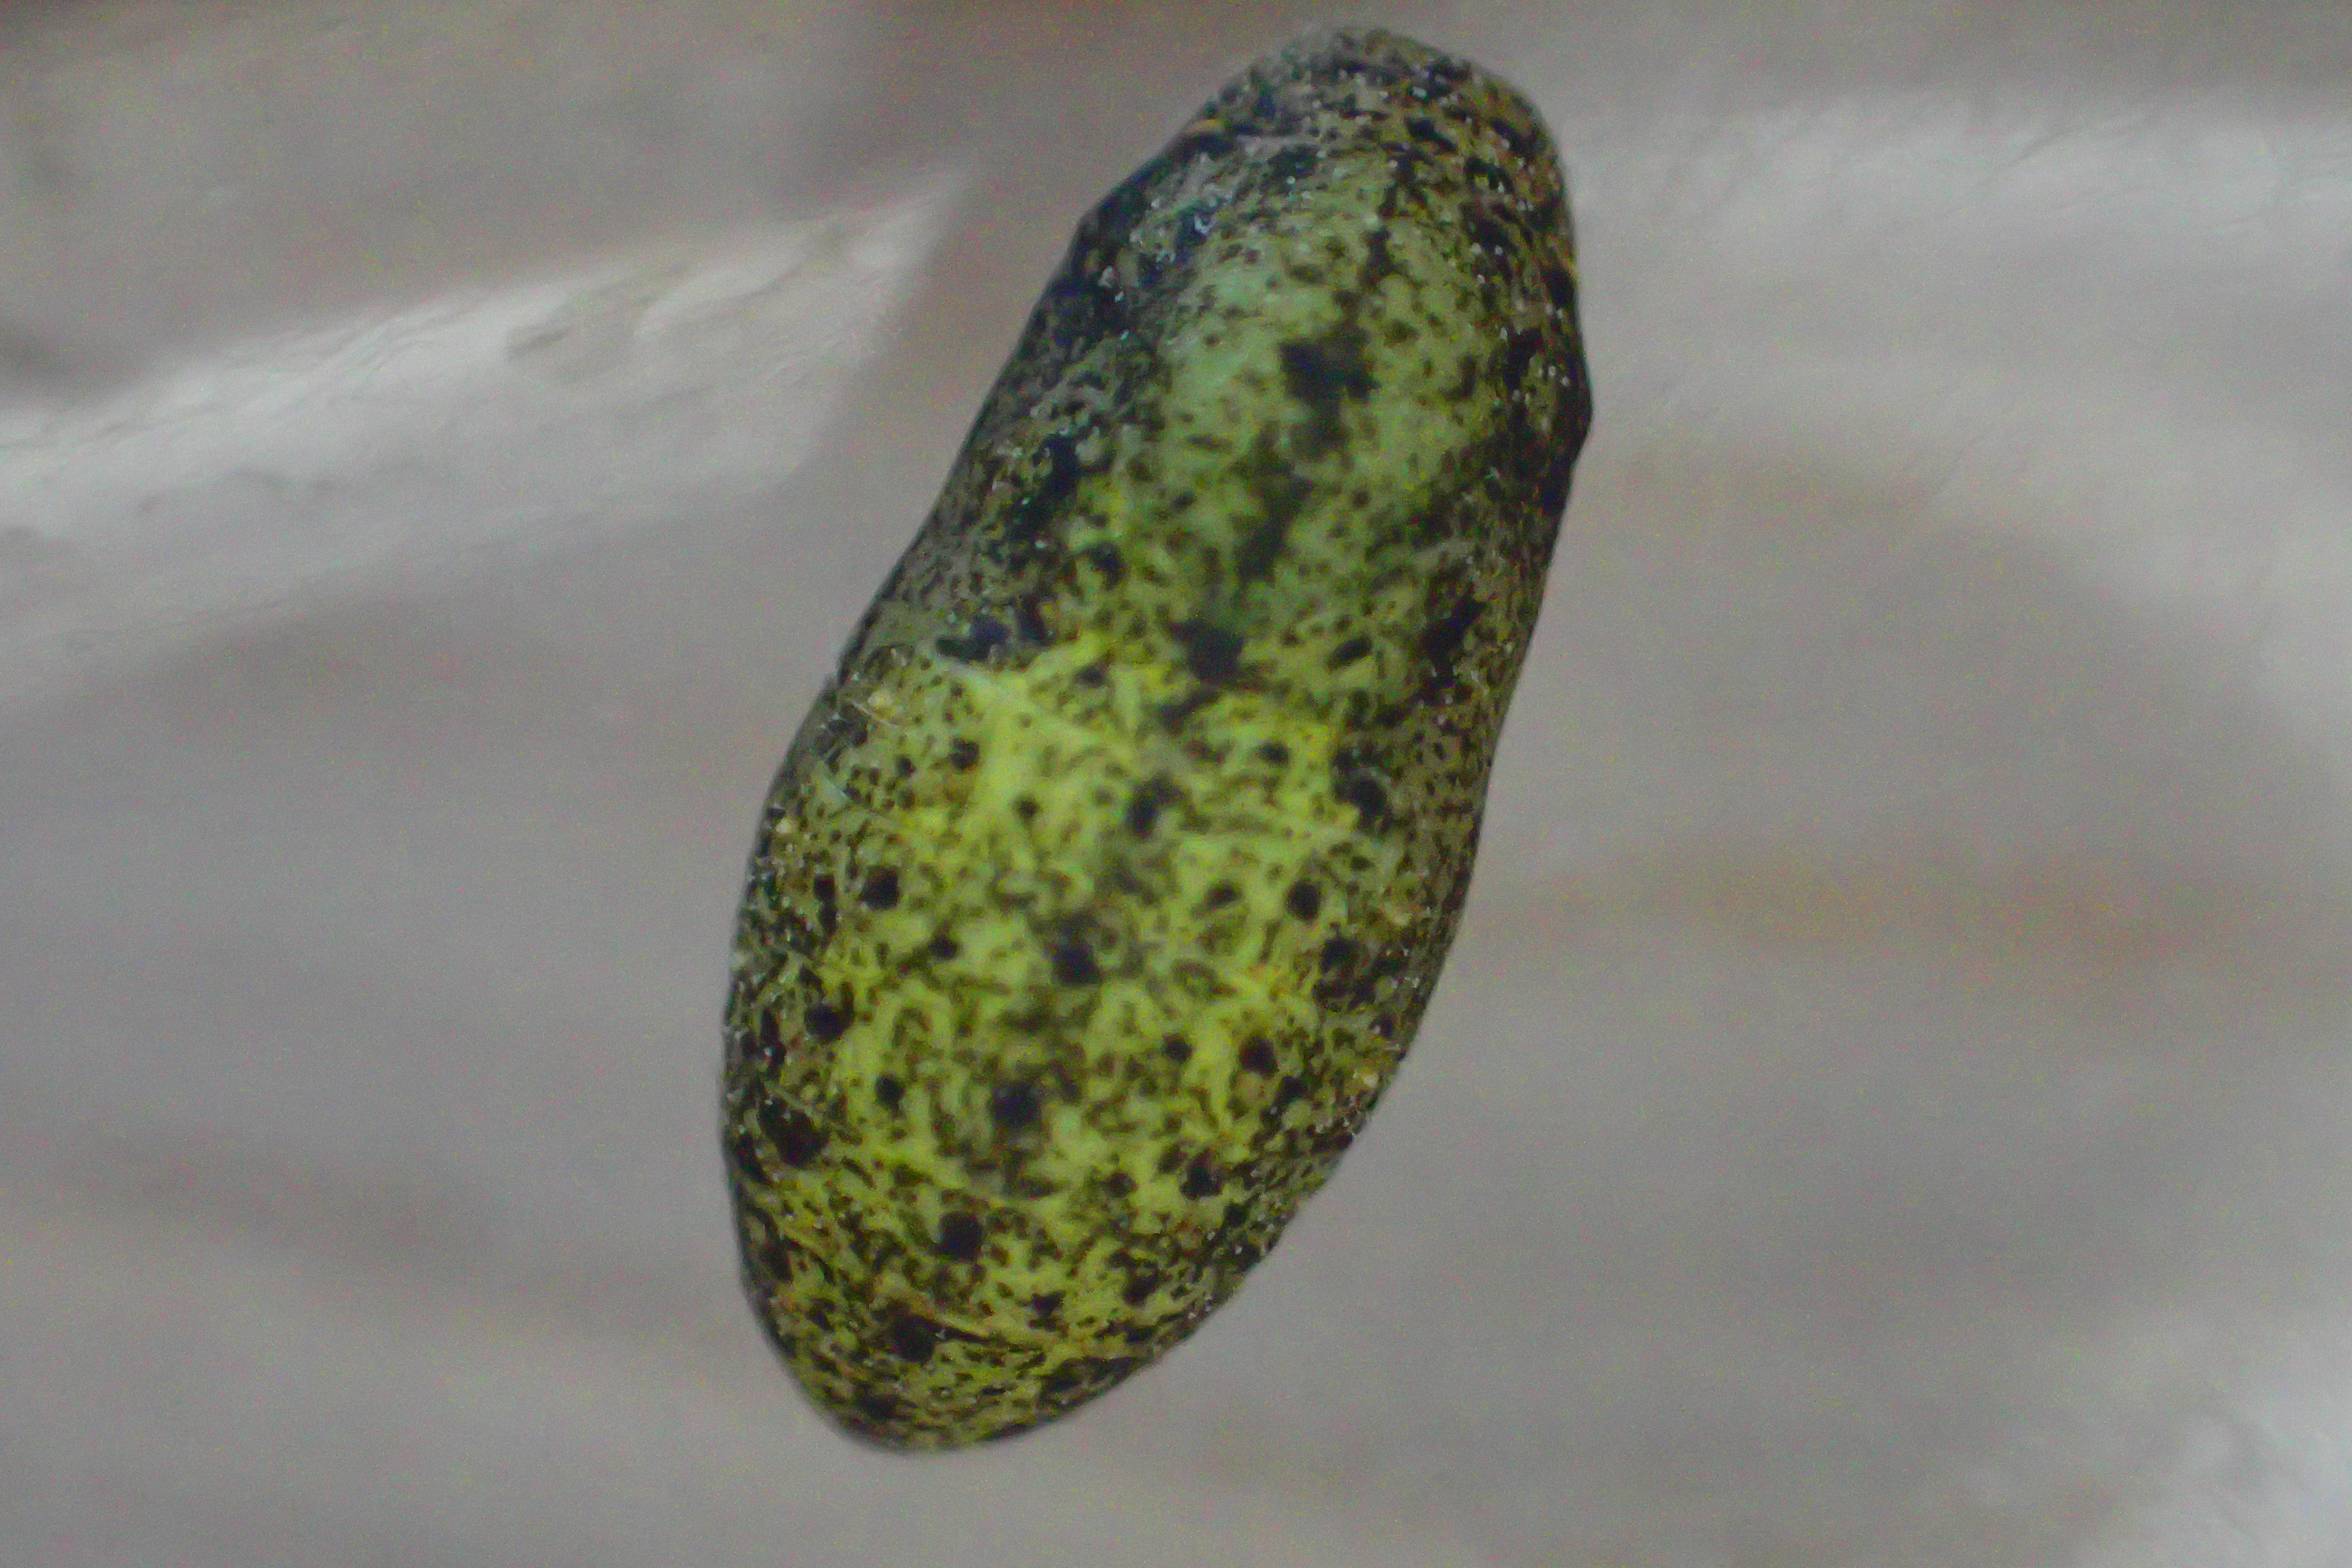
\includegraphics[width=5cm]{photo6/Larva4-pupa2.JPG}
  \end{center}
  \caption{幼虫4の蛹がここなしか黒く}
\end{figure}

\subsection{19時:異常無し}
幼虫4の蛹は明らかに黒くなってきた. 
幼虫5は, 相変わらずうろうろしているが, 蛹化する場所が決まらないのだろうか. 糞もほとんど出していない. 
幼虫6は, キッチンペーパーの上で静止したまま動かない. 脱皮が近い休眠状態か. 

\subsection{24時:異常無し}
幼虫5, 6ともにじっとして動かない. 死んでいる風ではないが少し気になる. 

\section{5/20の記録}
\subsection{10時:異常無し}
幼虫5は, 結局まだ葉を食べている. 幼虫6は全く動かない. 
幼虫4の蛹は, あれからほとんど変化がない. 

\subsection{11時:幼虫6が脱皮した}
あまりに動かないので心配していたが, ふと見ると移動しており, 脱皮の皮があった. 
アゲハなどと比べると結構ゆっくりであるようだ. 結局2日近く動いていなかった. 

\begin{figure}[htbp]
  \begin{center}
    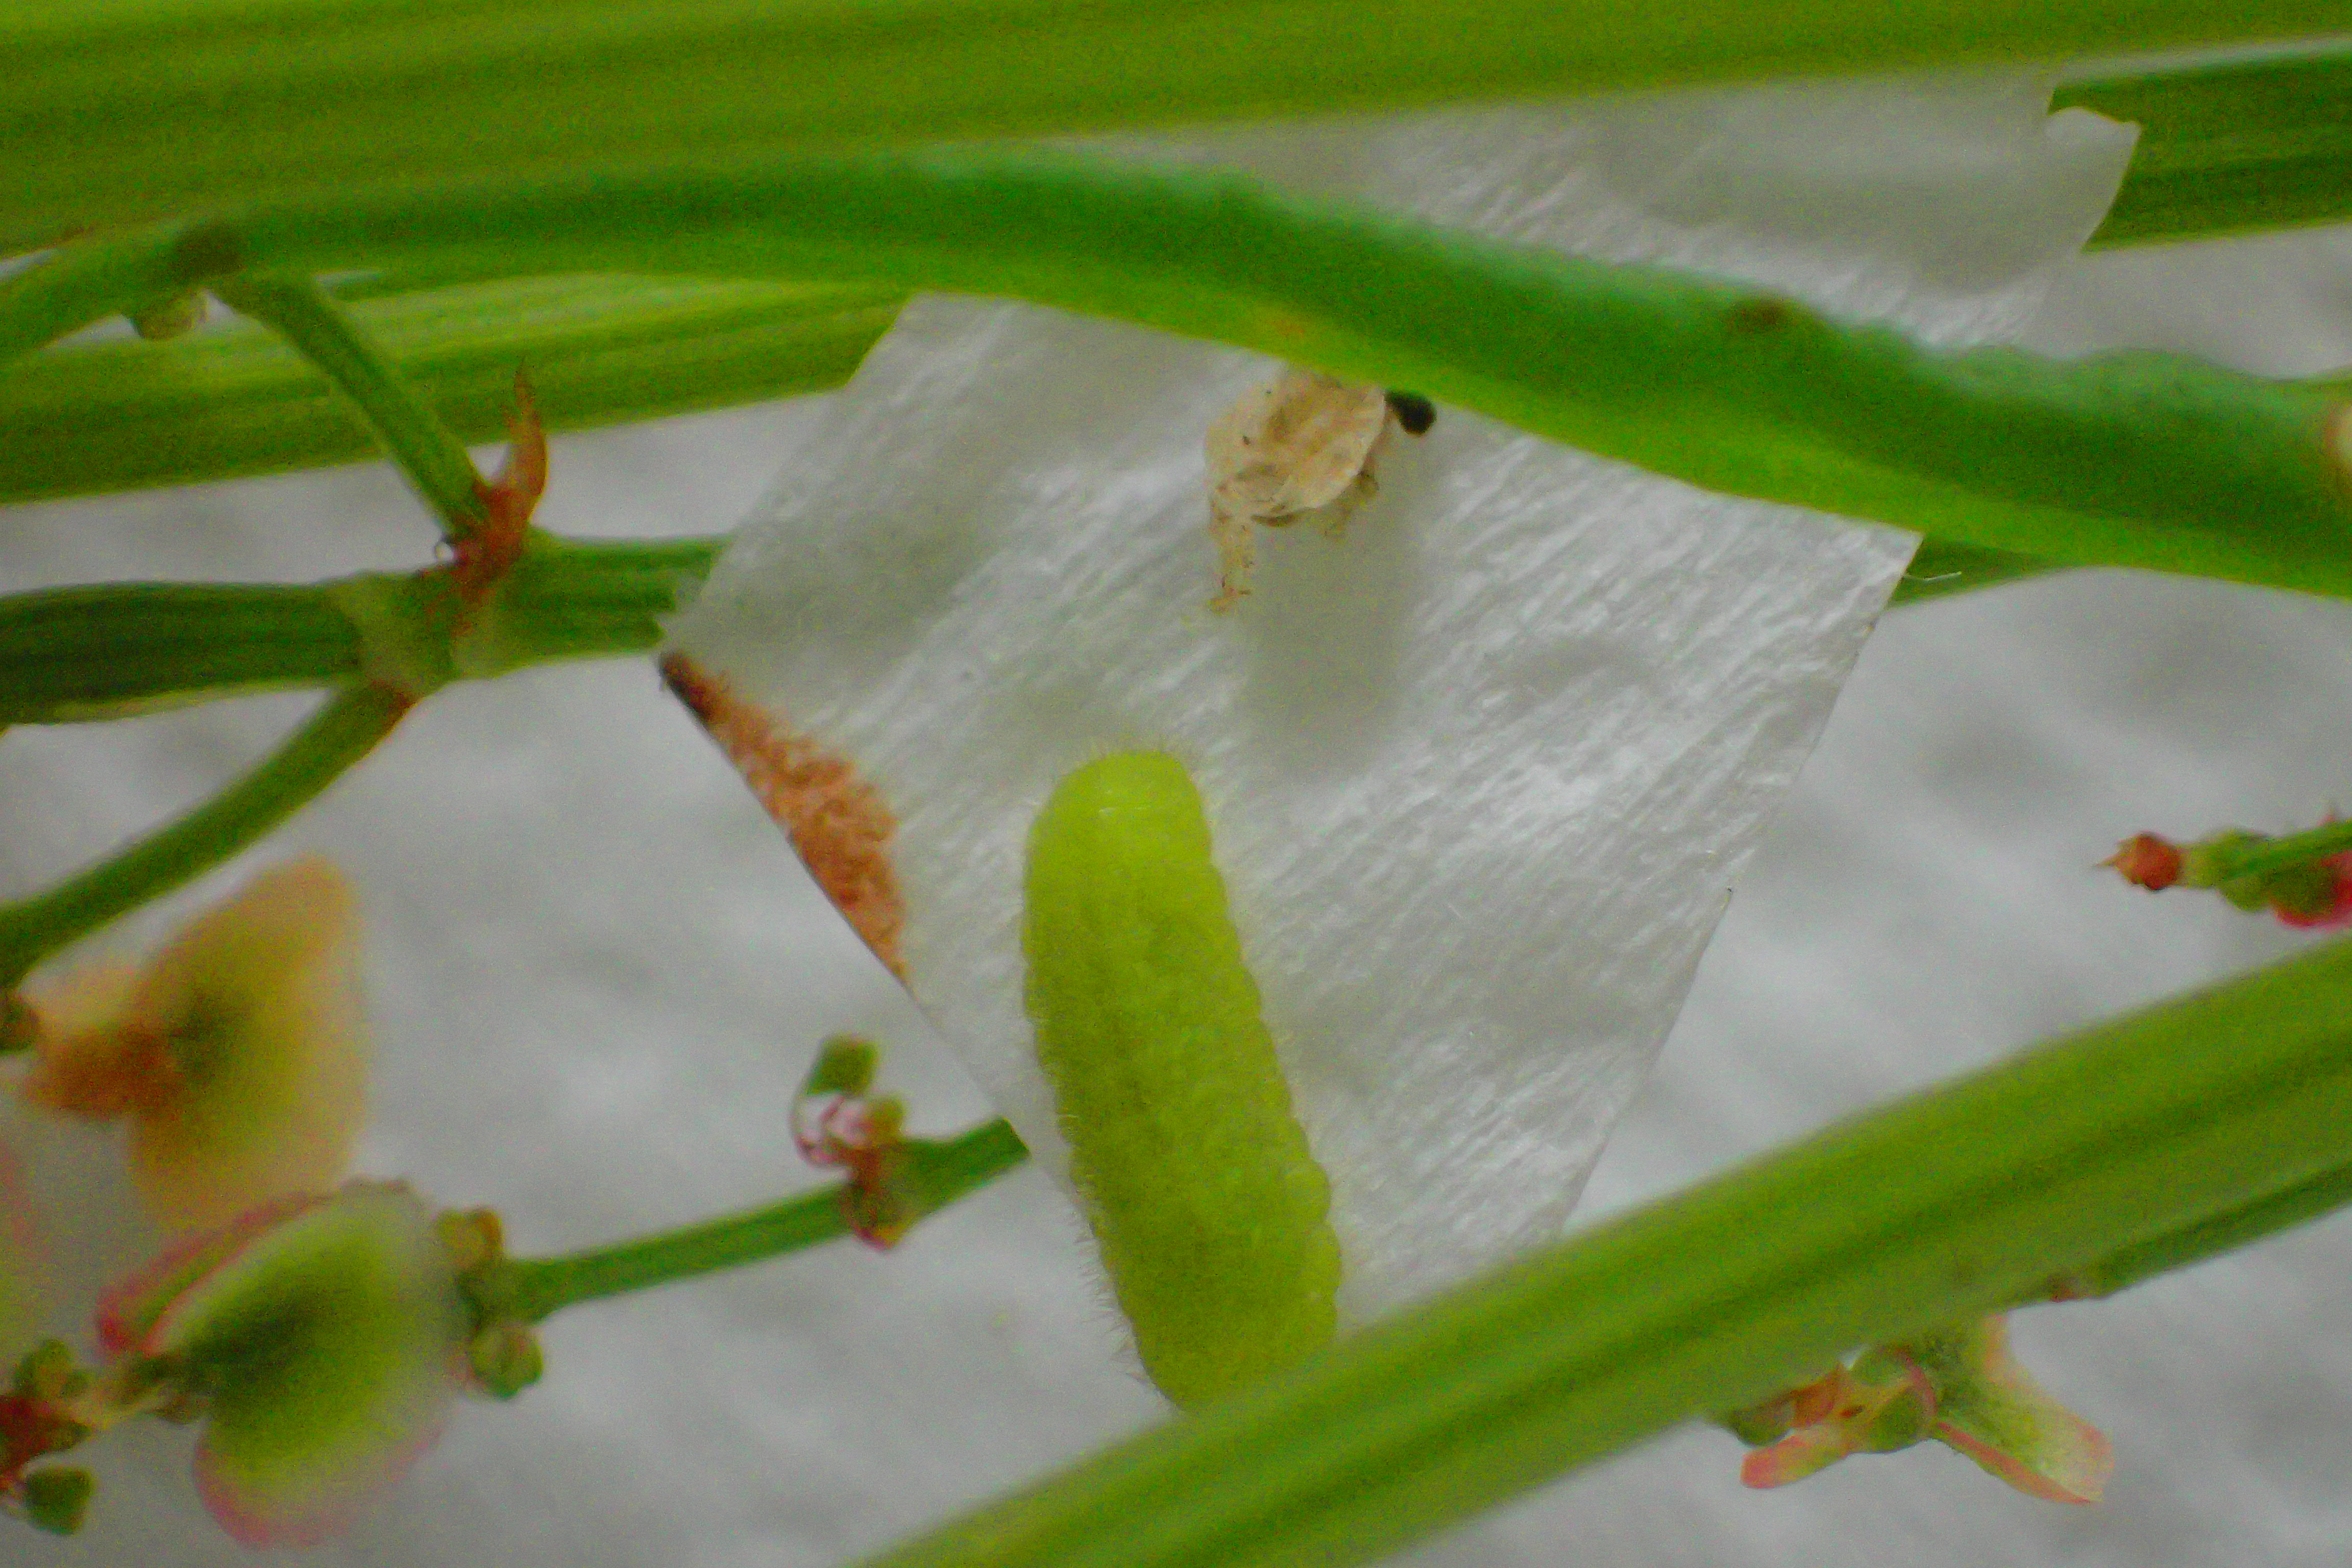
\includegraphics[width=5cm]{photo7/Larva6-Molting.JPG}
  \end{center}
  \caption{幼虫6が脱皮していた}
\end{figure}

\subsection{15時:幼虫6が動き出した}
脱皮後, しばらく動いていなかった幼虫6が移動を開始した. 脱皮後も, しばらく動かない期間があるようだ. 

\subsection{20時:異常無し}
幼虫5は相変わらず落ち着きなくあちこち移動して, そろそろ蛹化か, と思わせておいて結局葉を食っているという動作をつづけている. 幼虫6は, 食草の上を色々移動し, 糞も見られる. 

\begin{figure}[htbp]
  \begin{center}
    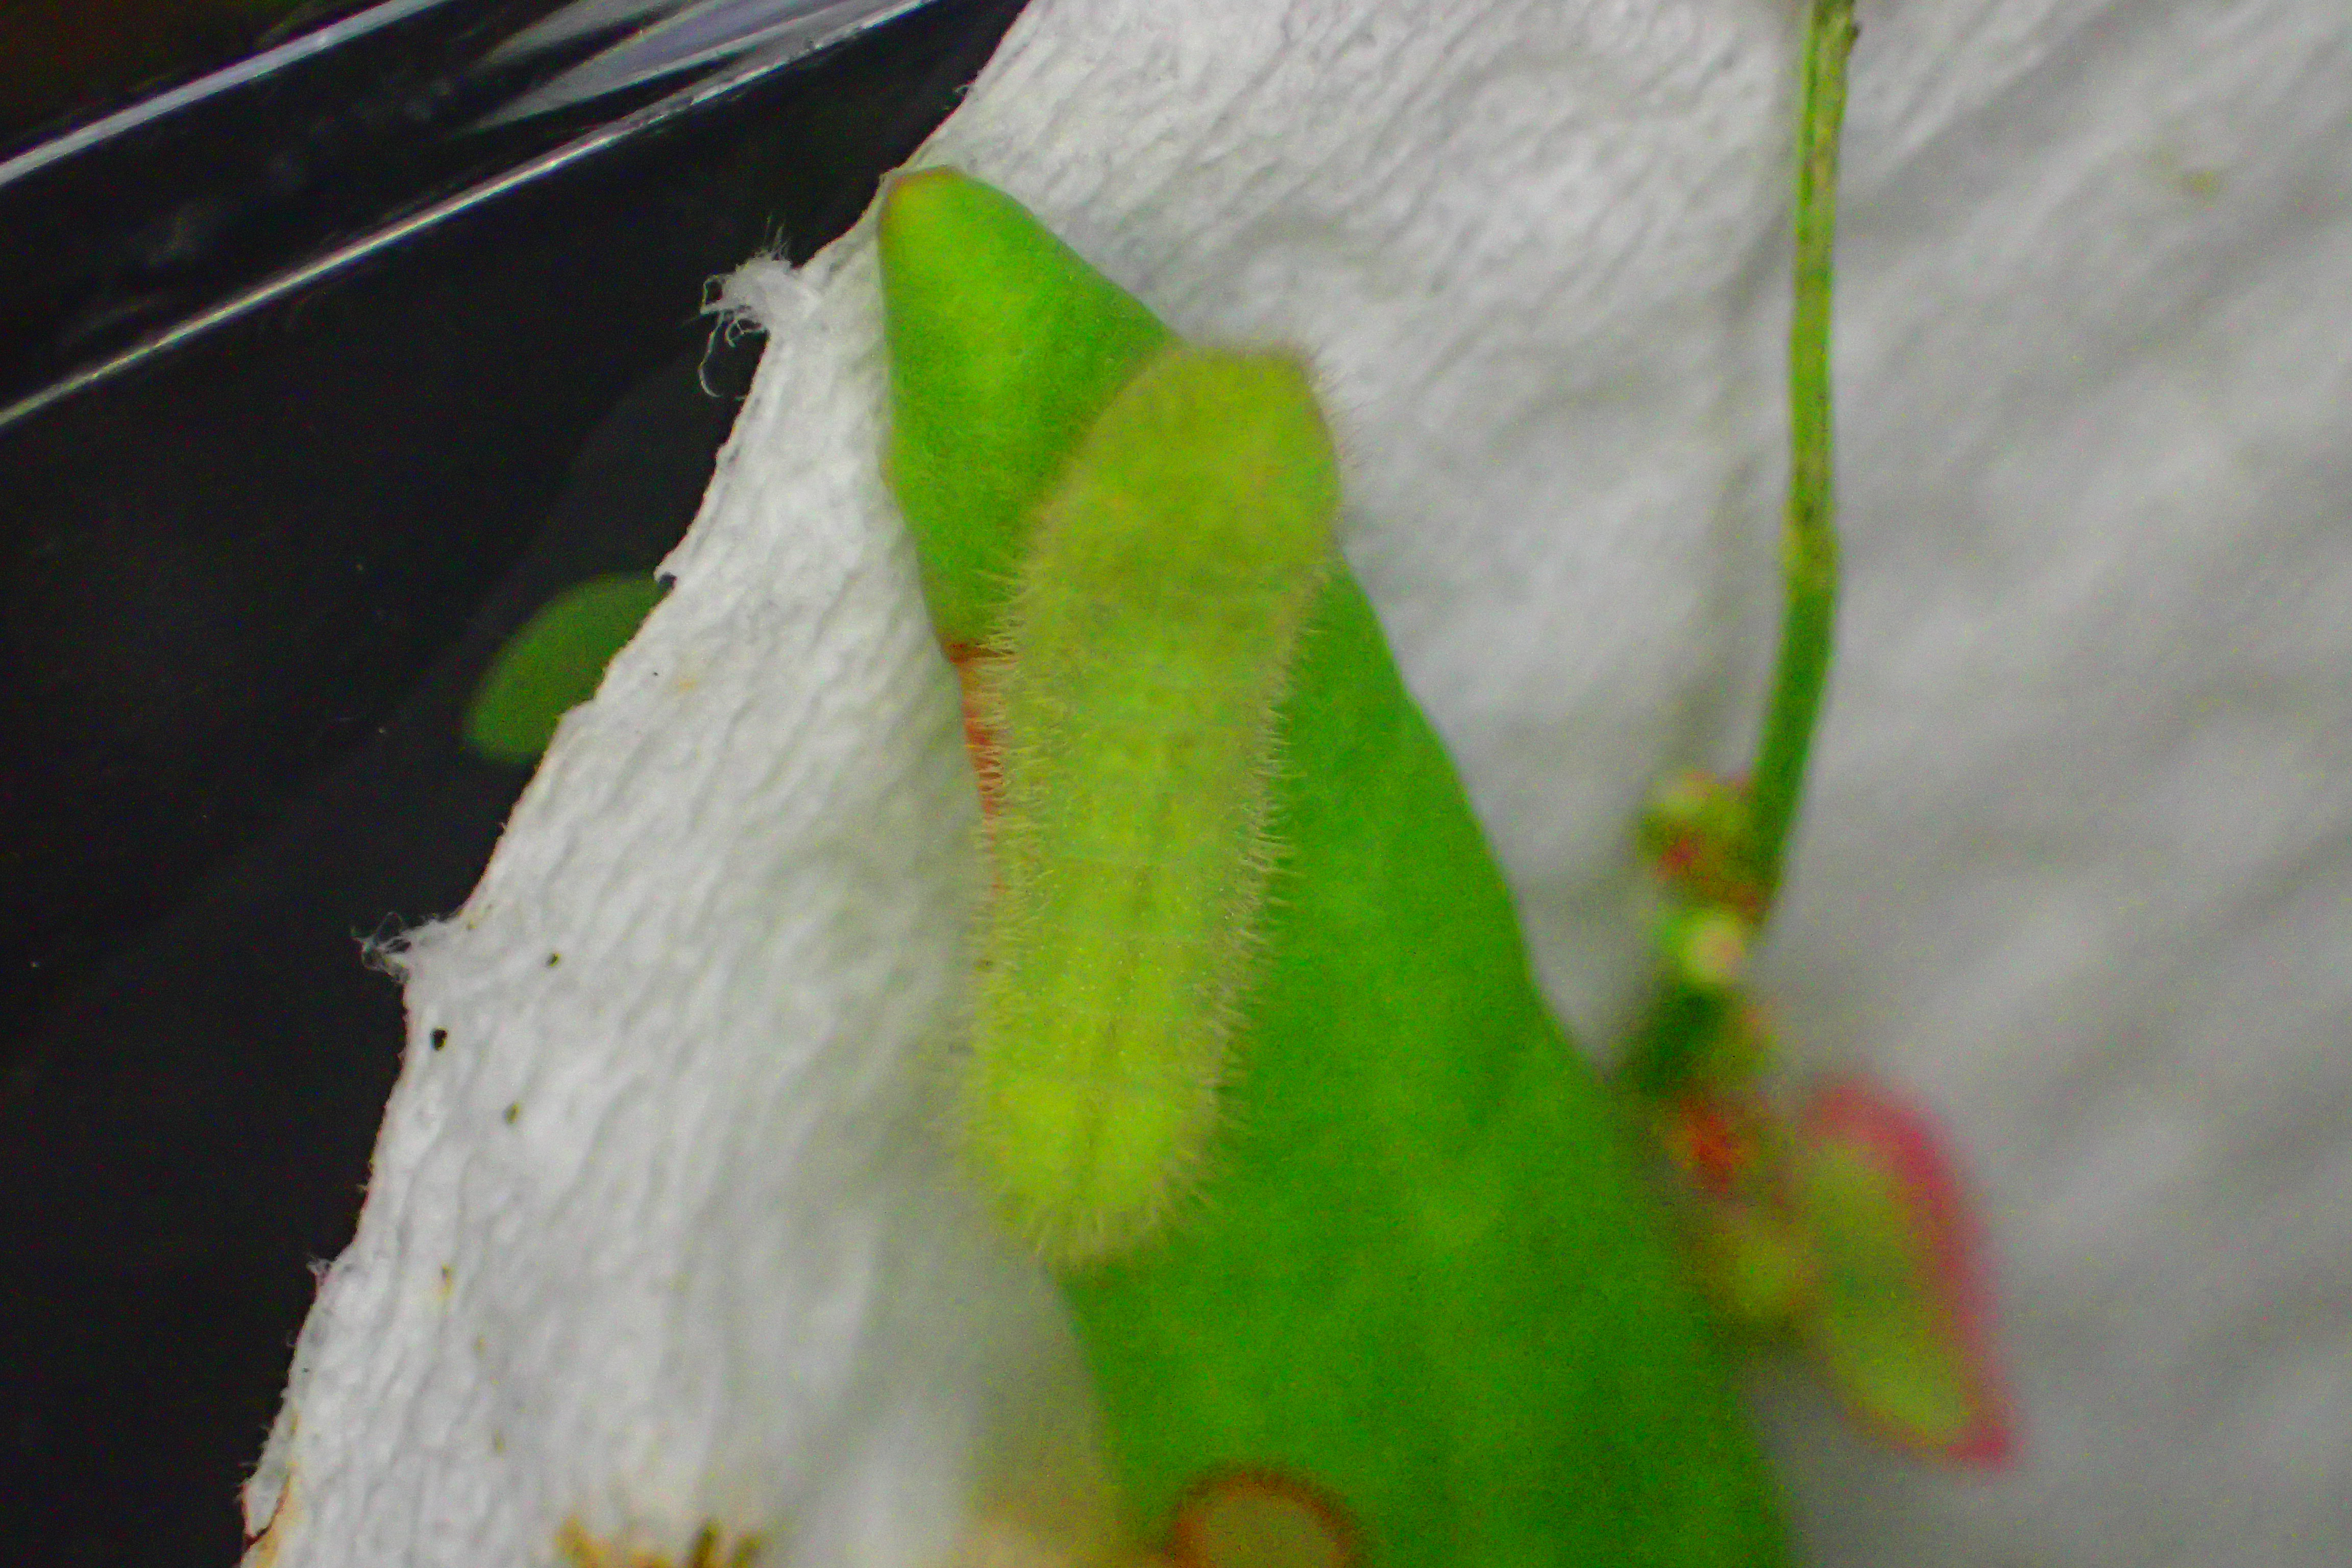
\includegraphics[width=5cm]{photo7/Larva6-Eating.JPG}
  \end{center}
  \caption{幼虫6が食草に移動した}
\end{figure}

\begin{figure}[htbp]
  \begin{center}
    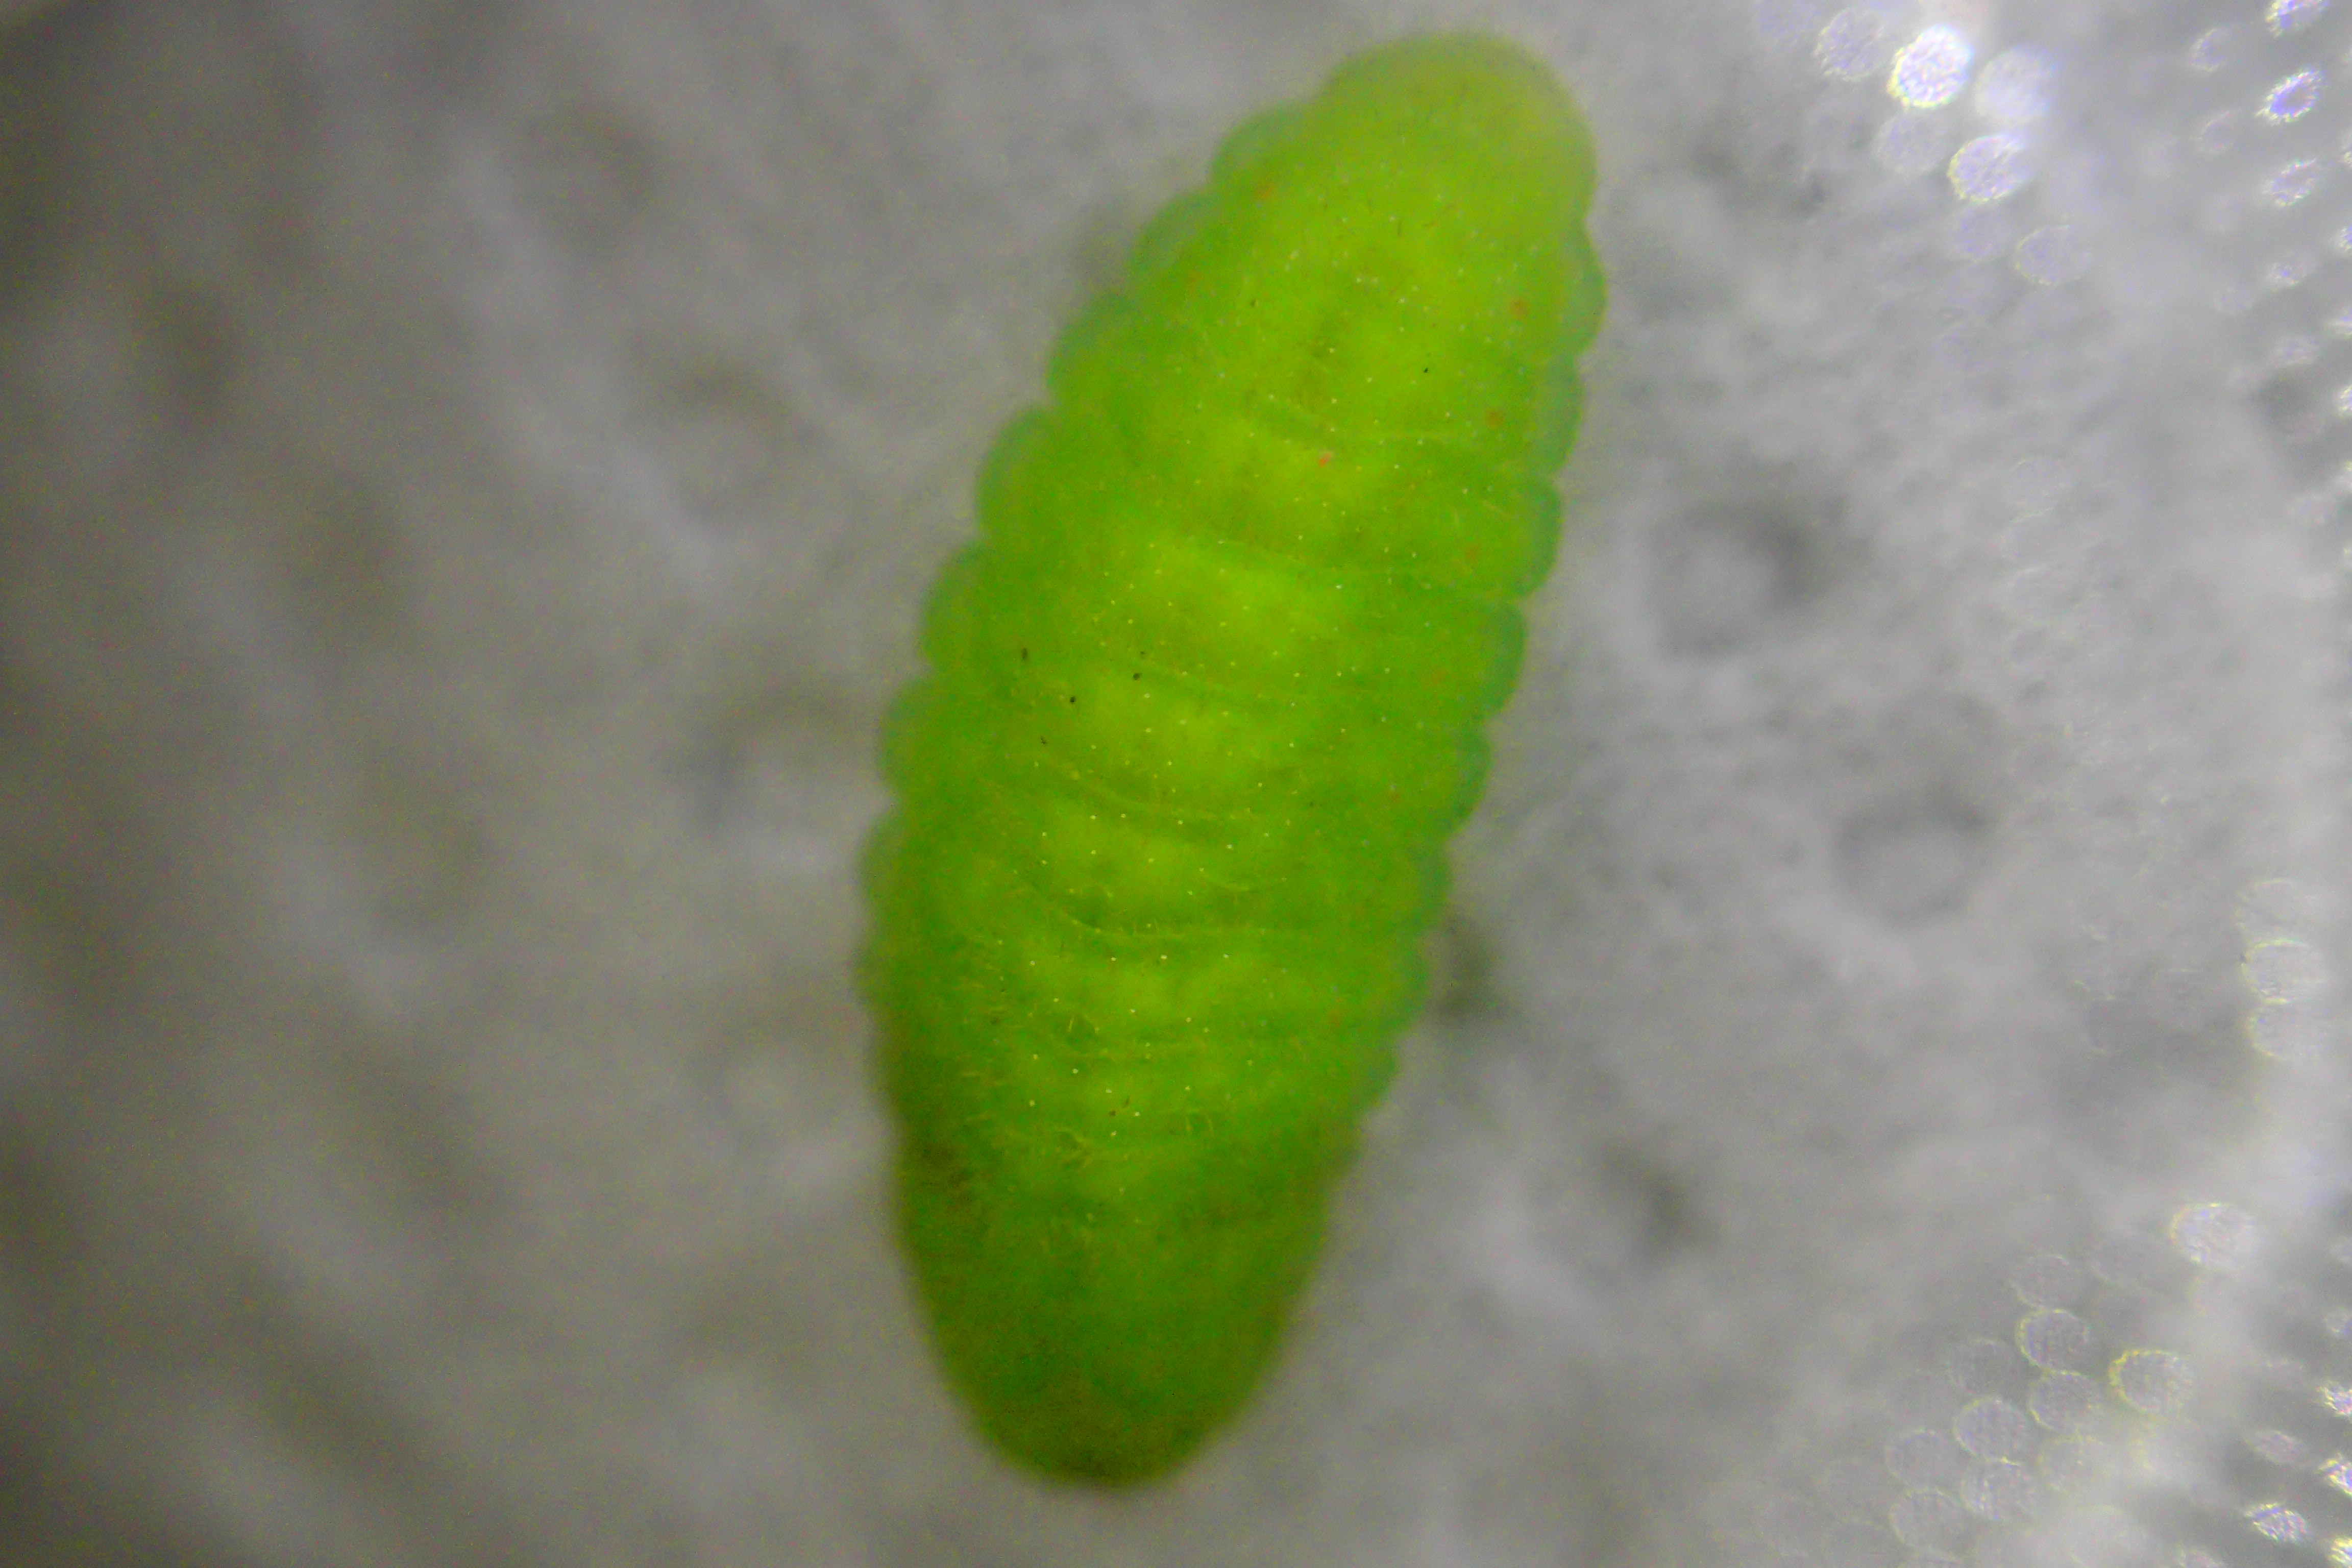
\includegraphics[width=5cm]{photo7/Larva5-Moving.JPG}
  \end{center}
  \caption{幼虫5がせわしなく動く}
\end{figure}

\section{5/21の記録}
\subsection{22時:幼虫5はようやく前蛹っぽい}
幼虫5が, キッチンペーパーのまがりによりできたくぼみの中で小さく縮こまったまま動かなくなった. 
ようやく前蛹か. 
幼虫6は, 脱皮後の休息も終わって, 忙しなく動き回っている. 

\begin{figure}[htbp]
  \begin{center}
    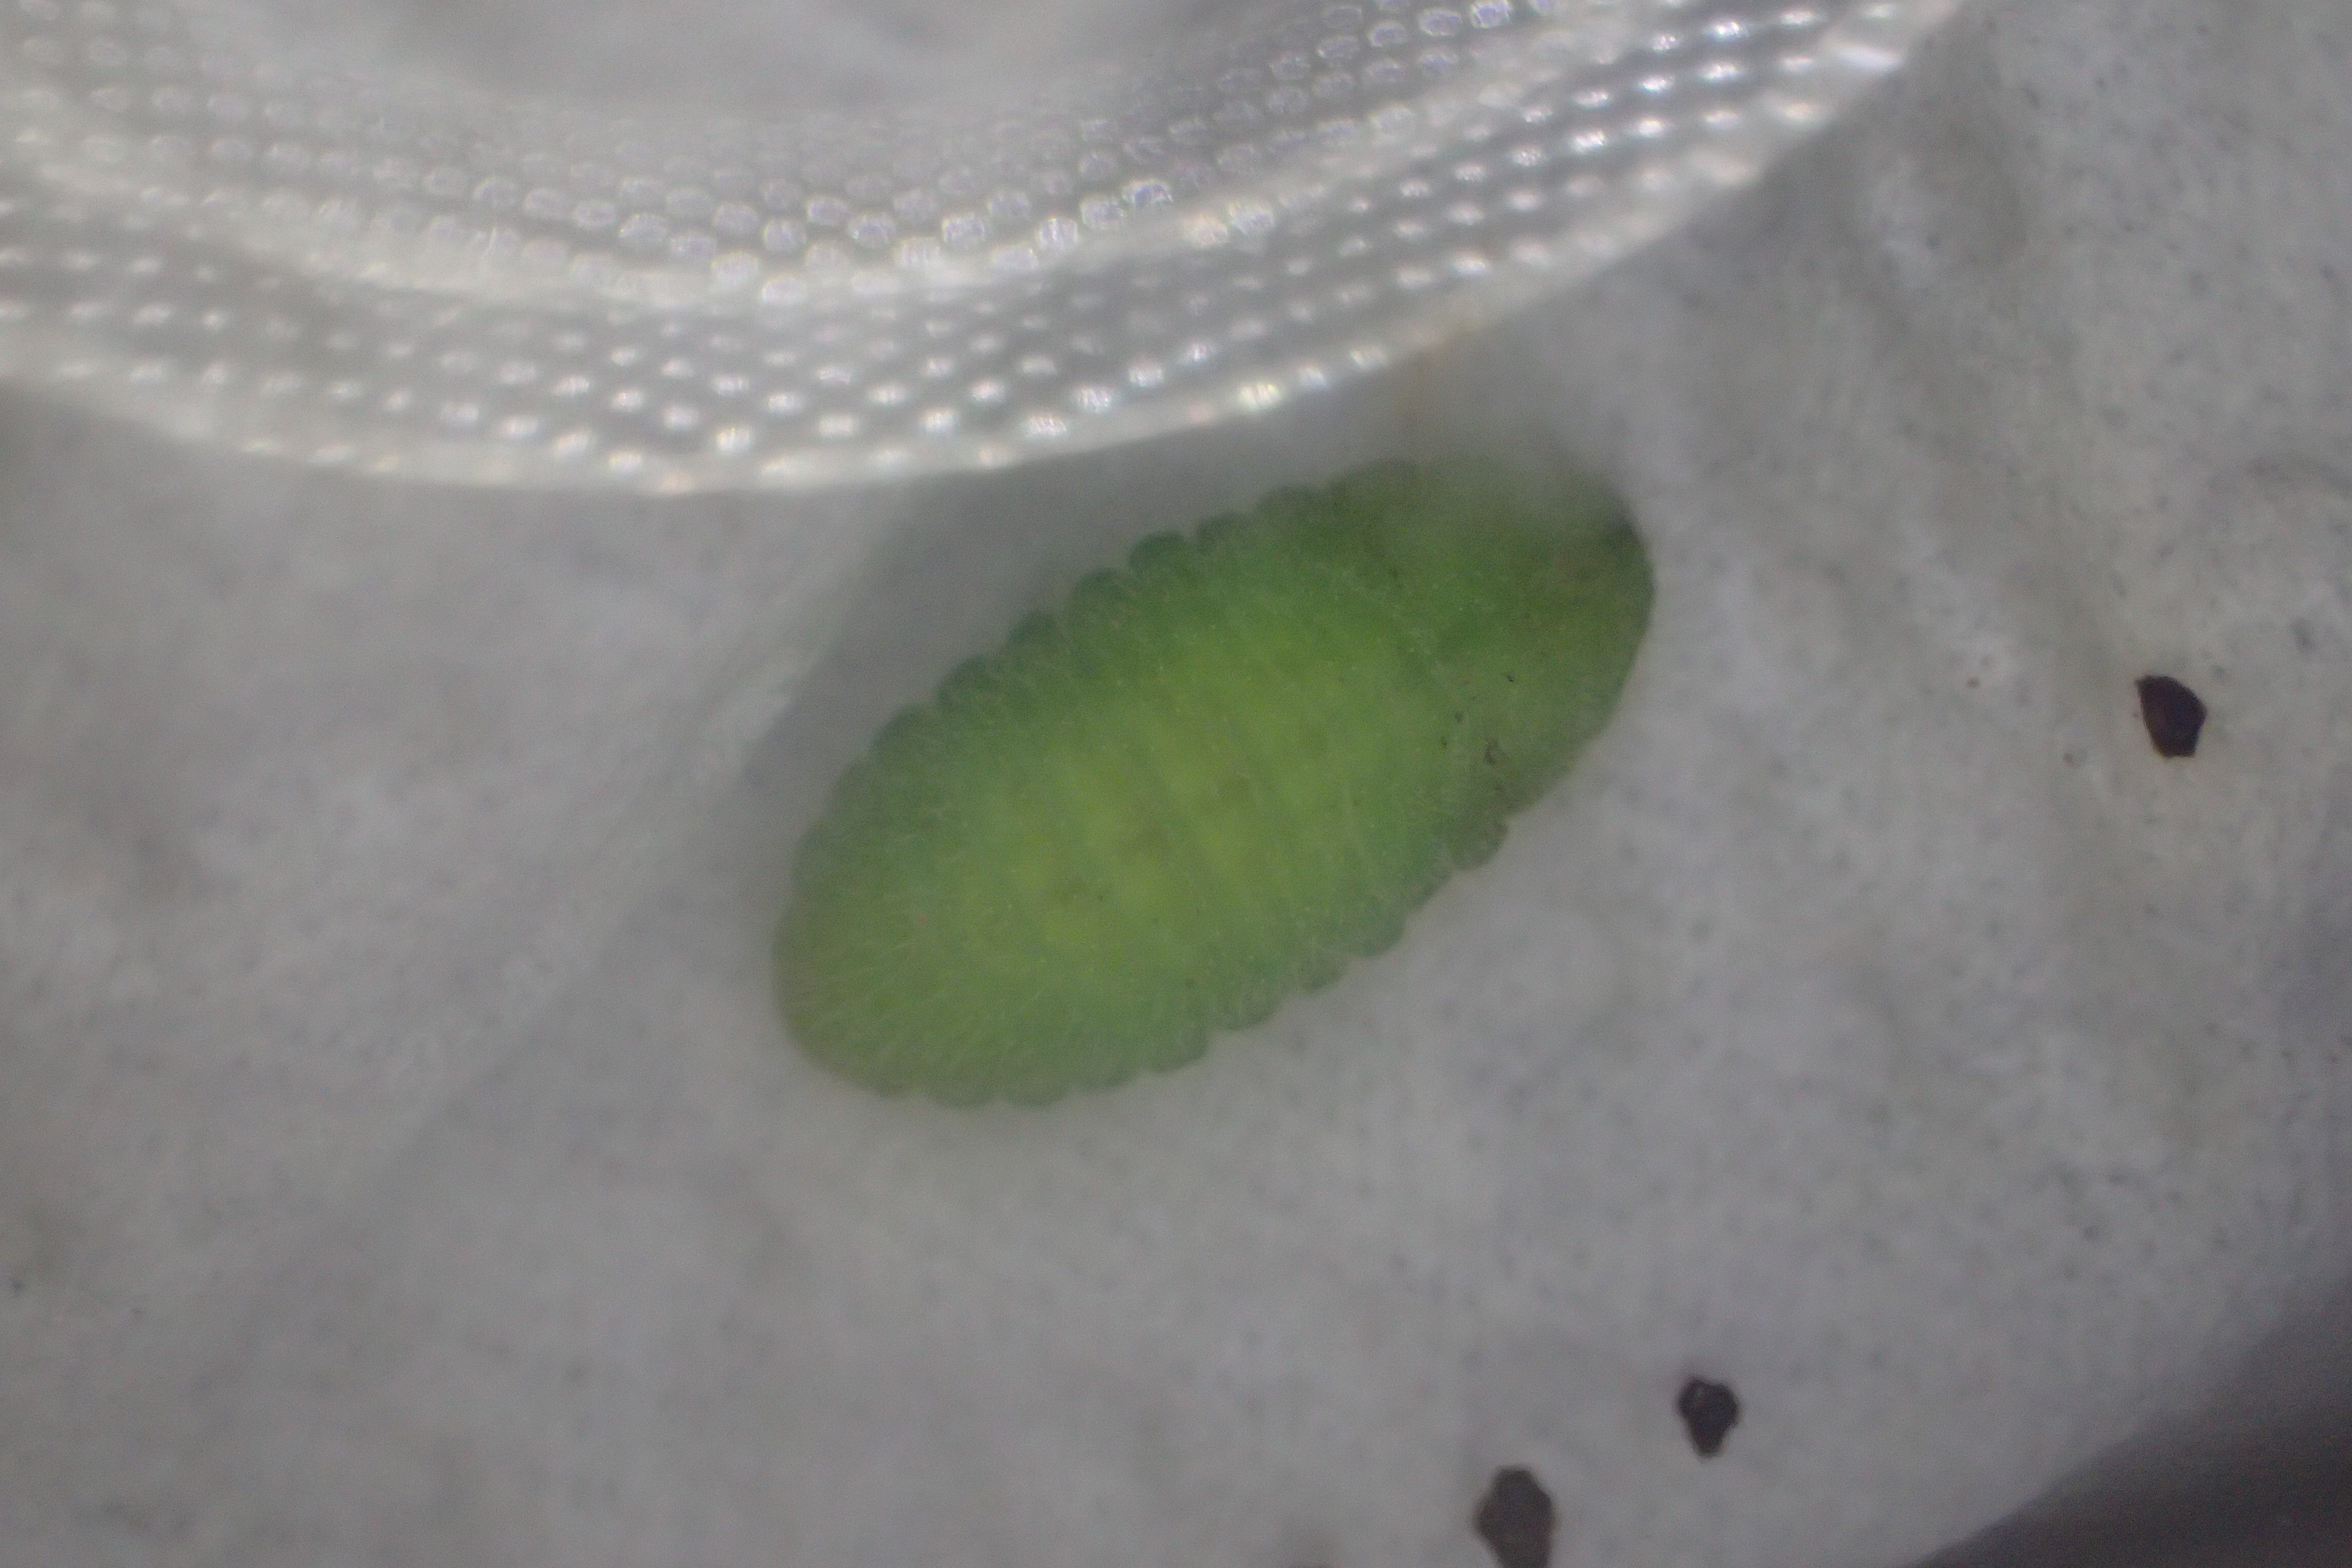
\includegraphics[width=5cm]{photo8/Larva5-prePupa.JPG}
  \end{center}
  \caption{幼虫5が前蛹}
\end{figure}

\section{5/22の記録}
特段変化は何も無し

\section{5/23の記録}
\subsection{10時:幼虫5の前蛹が少し変化}
より背中が丸くなり, 筋が目立つようになってきて, 若干黄色味を帯びてきた. 蛆虫が出てきた時の色とは違う. 
幼虫6は, 水分糞をだしたようだ. 終齢幼虫の蛹化前でなくとも, あるようだ. 

\begin{figure}[htbp]
  \begin{center}
    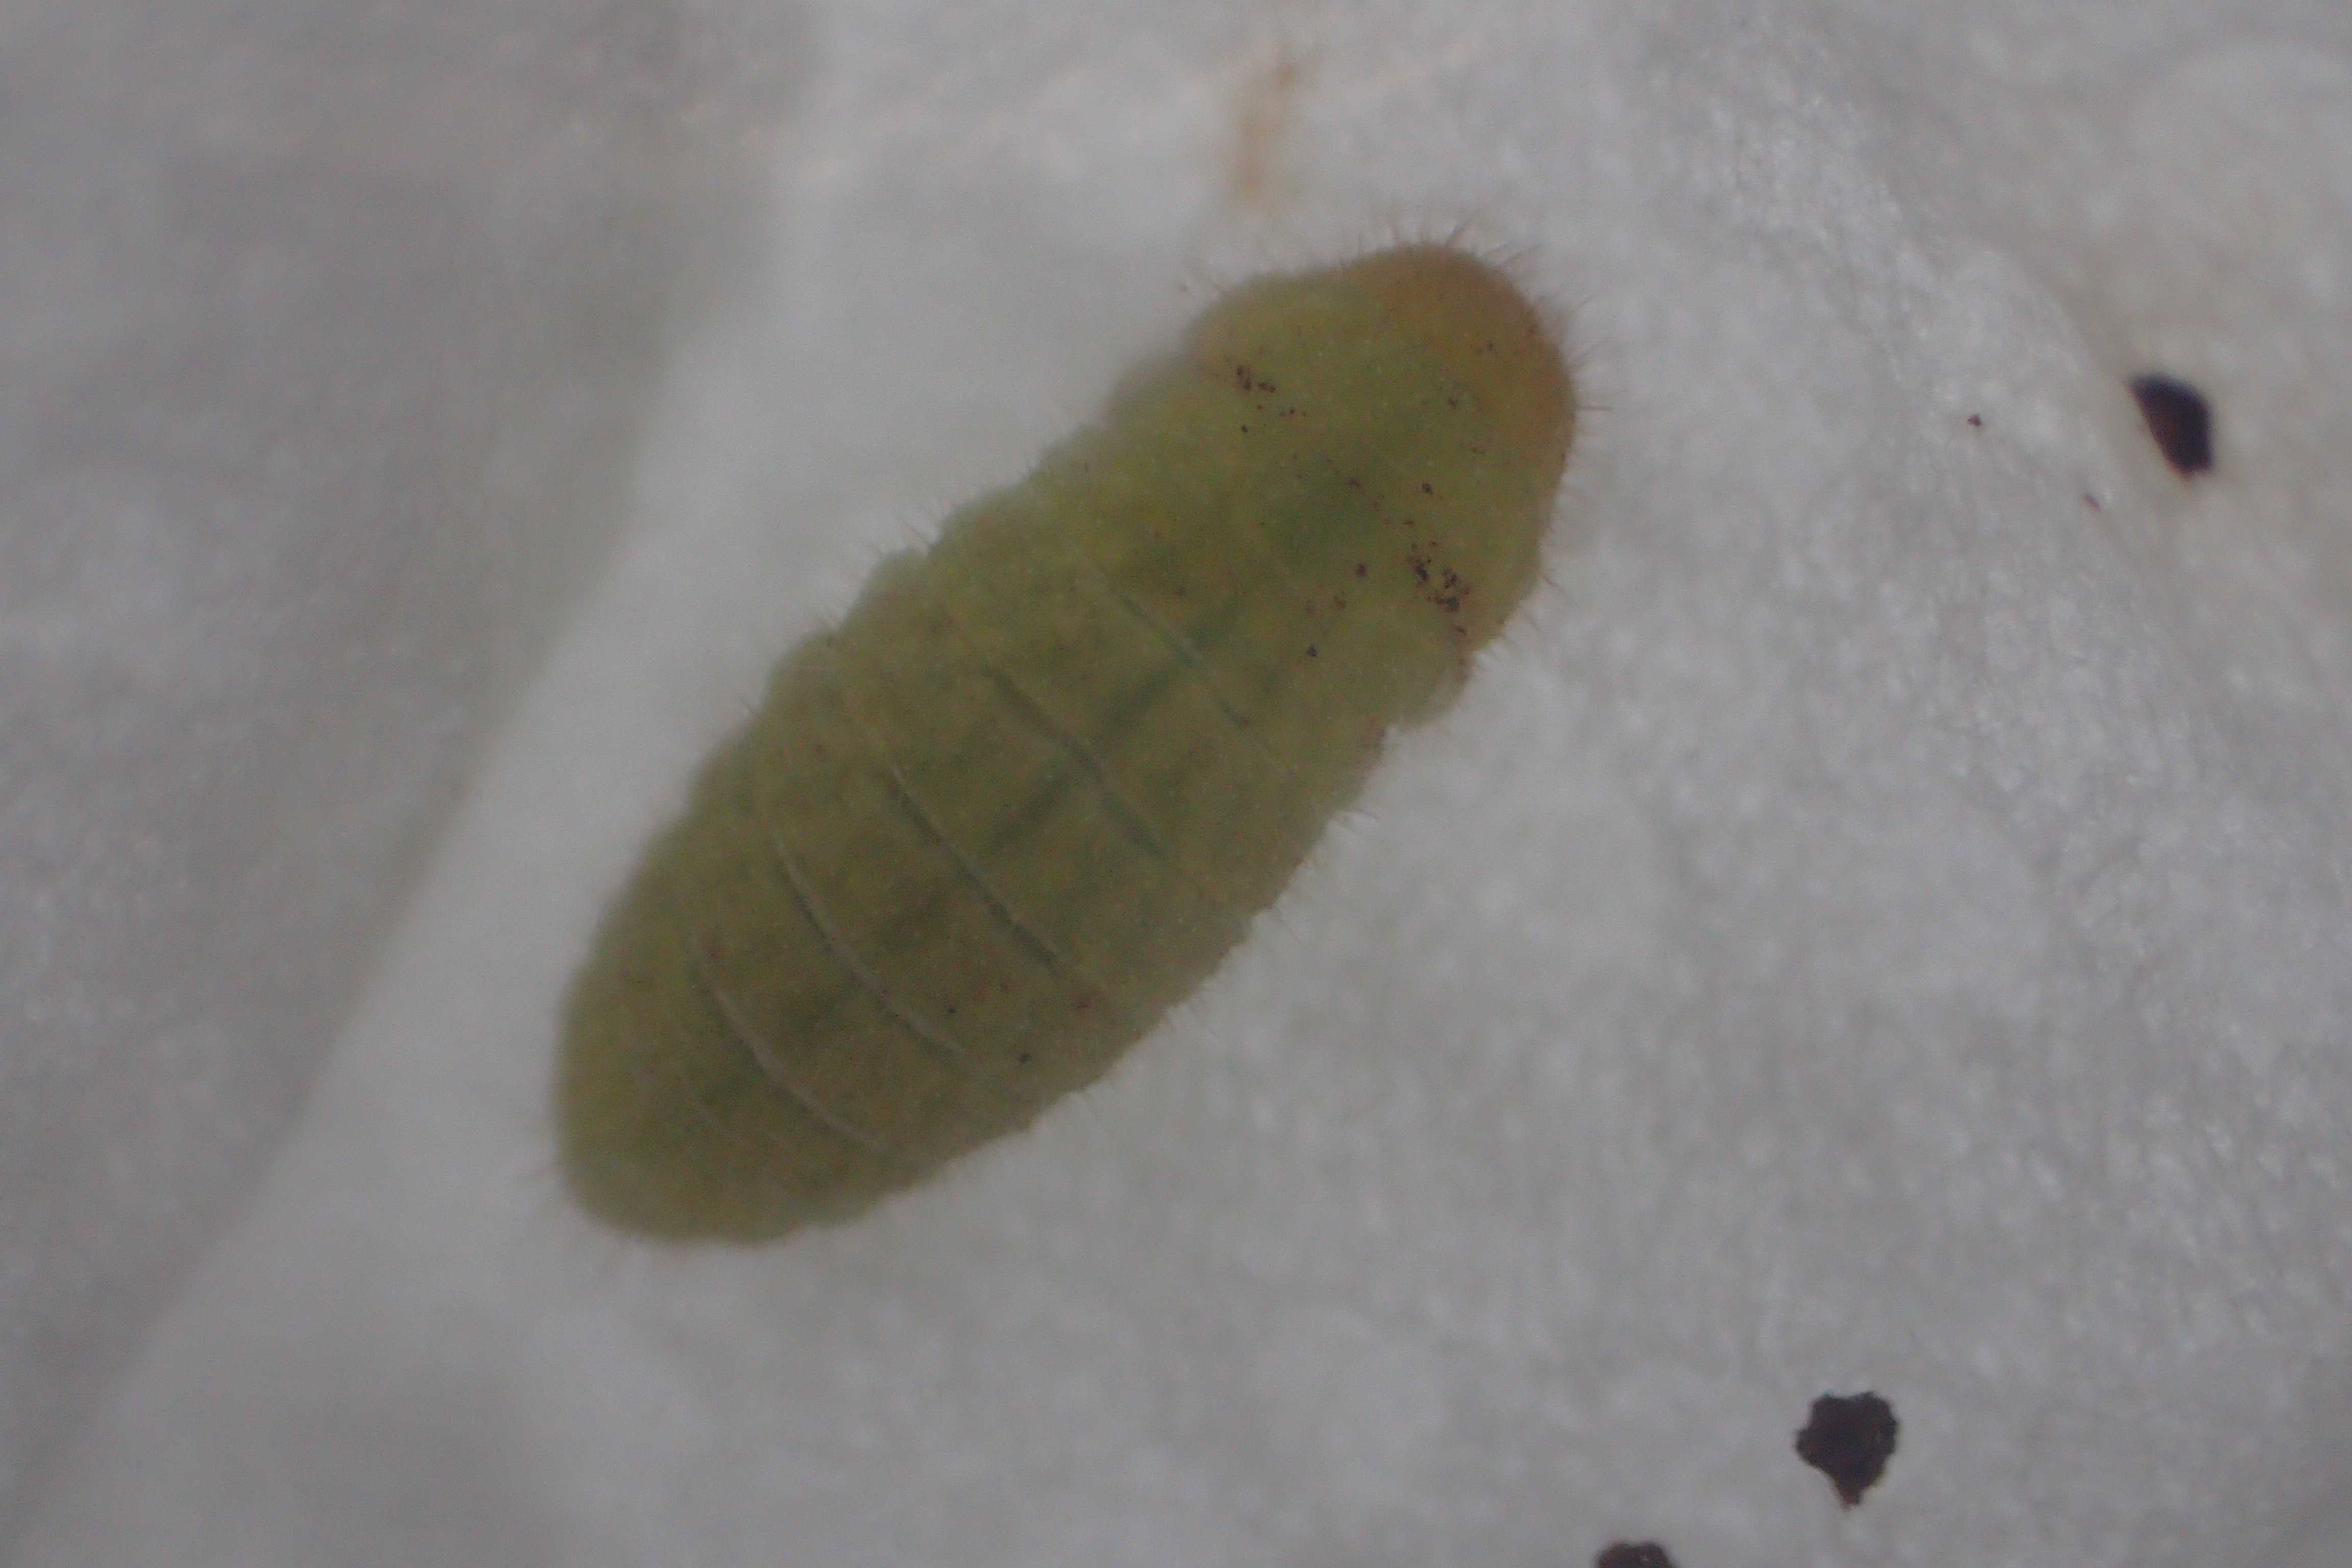
\includegraphics[width=5cm]{photo9/Larva5-prePupa.JPG}
  \end{center}
  \caption{幼虫5の前蛹が変化してきた}
\end{figure}

\subsection{12時:幼虫5が蛹化}
目を離した隙に脱皮が終了し, 完全に蛹になっていた.

\begin{figure}[htbp]
  \begin{center}
    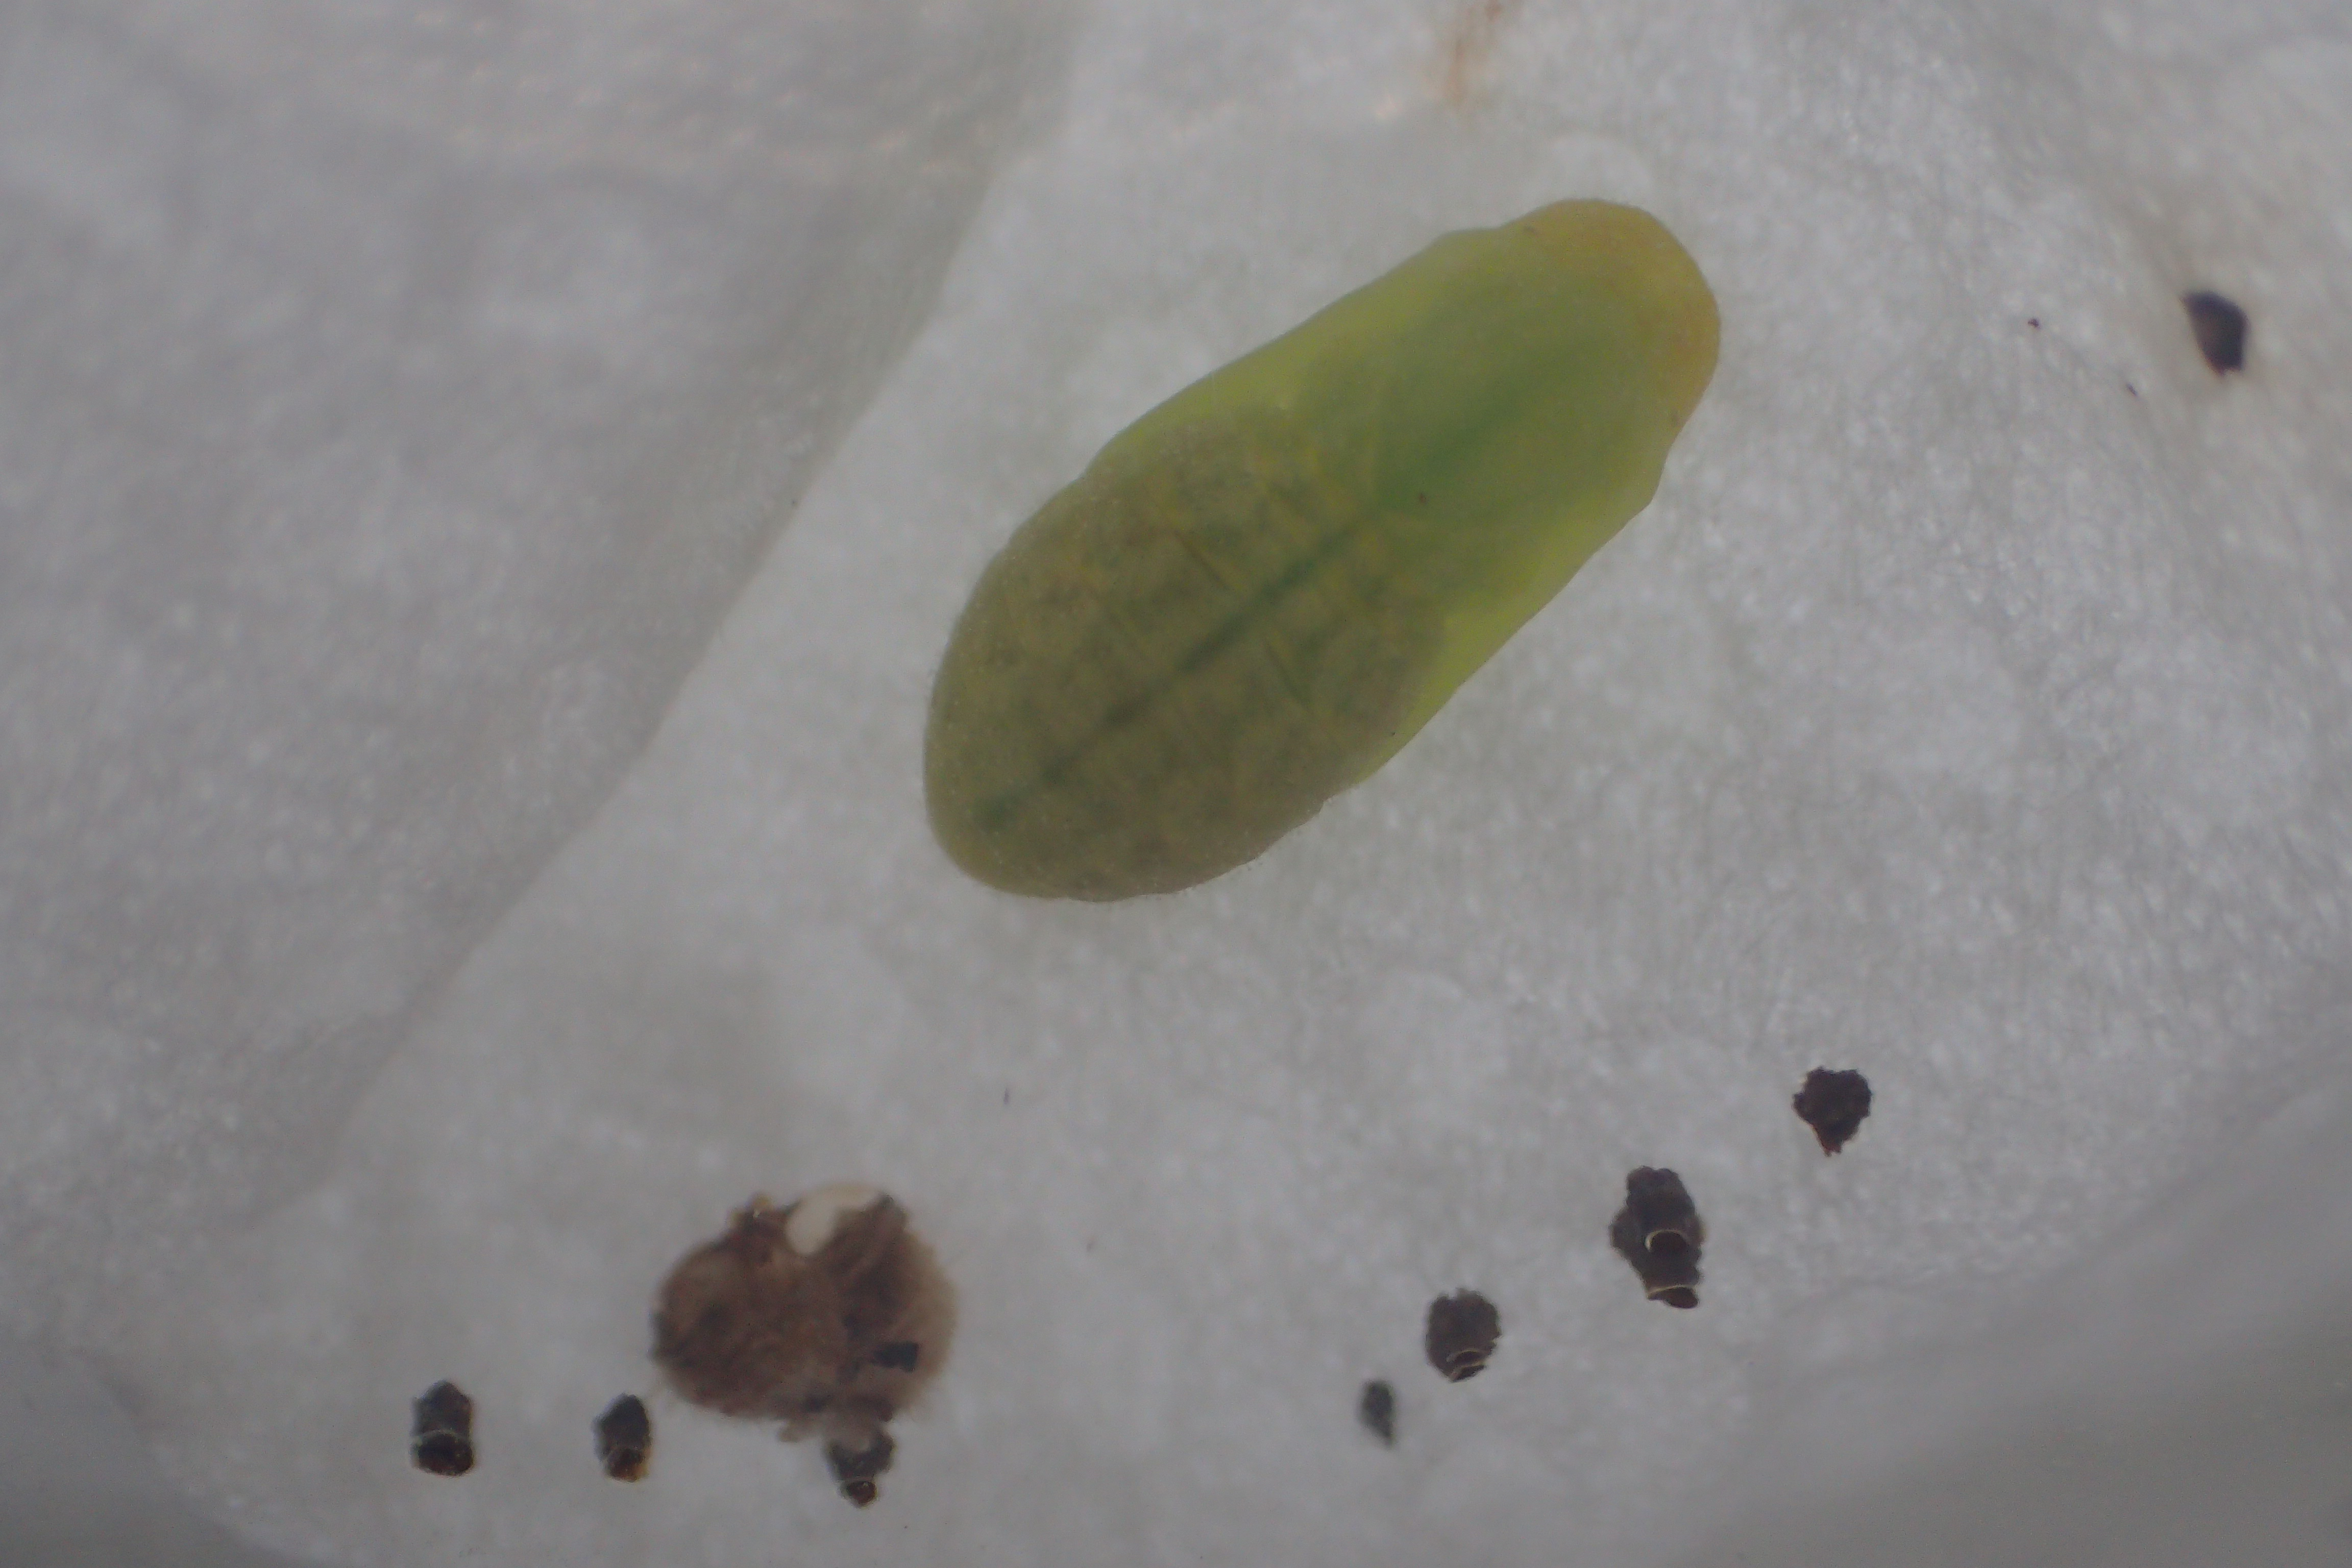
\includegraphics[width=5cm]{photo9/Larva5-pupa.JPG}
  \end{center}
  \caption{幼虫5が蛹になった}
\end{figure}

\subsection{18時:幼虫6が動かない}
幼虫6が, 水様の糞を出して以降, まったく動かない. 少しきになるが, 幼虫1,2 の時の反省と, 脱皮時の休眠期間を考慮し, 
変に触らず見守ることとする. 

\section{5/24の記録}
\subsection{23時の記録}
幼虫6はまったく動かない上に, どんどん小さくなっていく. おそらく死んでいるのであろう. 
幼虫1,2は, 高温多湿で殺してしまったが, 幼虫6については, 思い当たる節としては, 脱皮直後に, 2日ほど, 
気温がやたら下がった日があり, これの影響ではないかと考えられる. 
脱皮直後という極めて体力が消耗している時の気温の変化に耐えられなかったのだろうか. 
人間で言うところのいわゆる風邪とでもいうのか. 非常に弱い. 
やはり, 羽化までの成功率をあげるには, 温湿度の管理, UVA程度のほどよい紫外線の照射など, かなり精密に
環境制御をしてやらないといけないか. 

\section{5/27の記録}
幼虫6はもう完全にかさかさになり, ごみのようになってしまった. 
幼虫4の蛹が, 色が突然黒くなった. 羽化の前兆だ. 
羽化に備えて, 蛹の周りのガラスでは足場として不安定なので, キッチンペーパーで足場を作成してやった. 明日には羽化するだろう. 


\begin{figure}[htbp]
  \begin{center}
    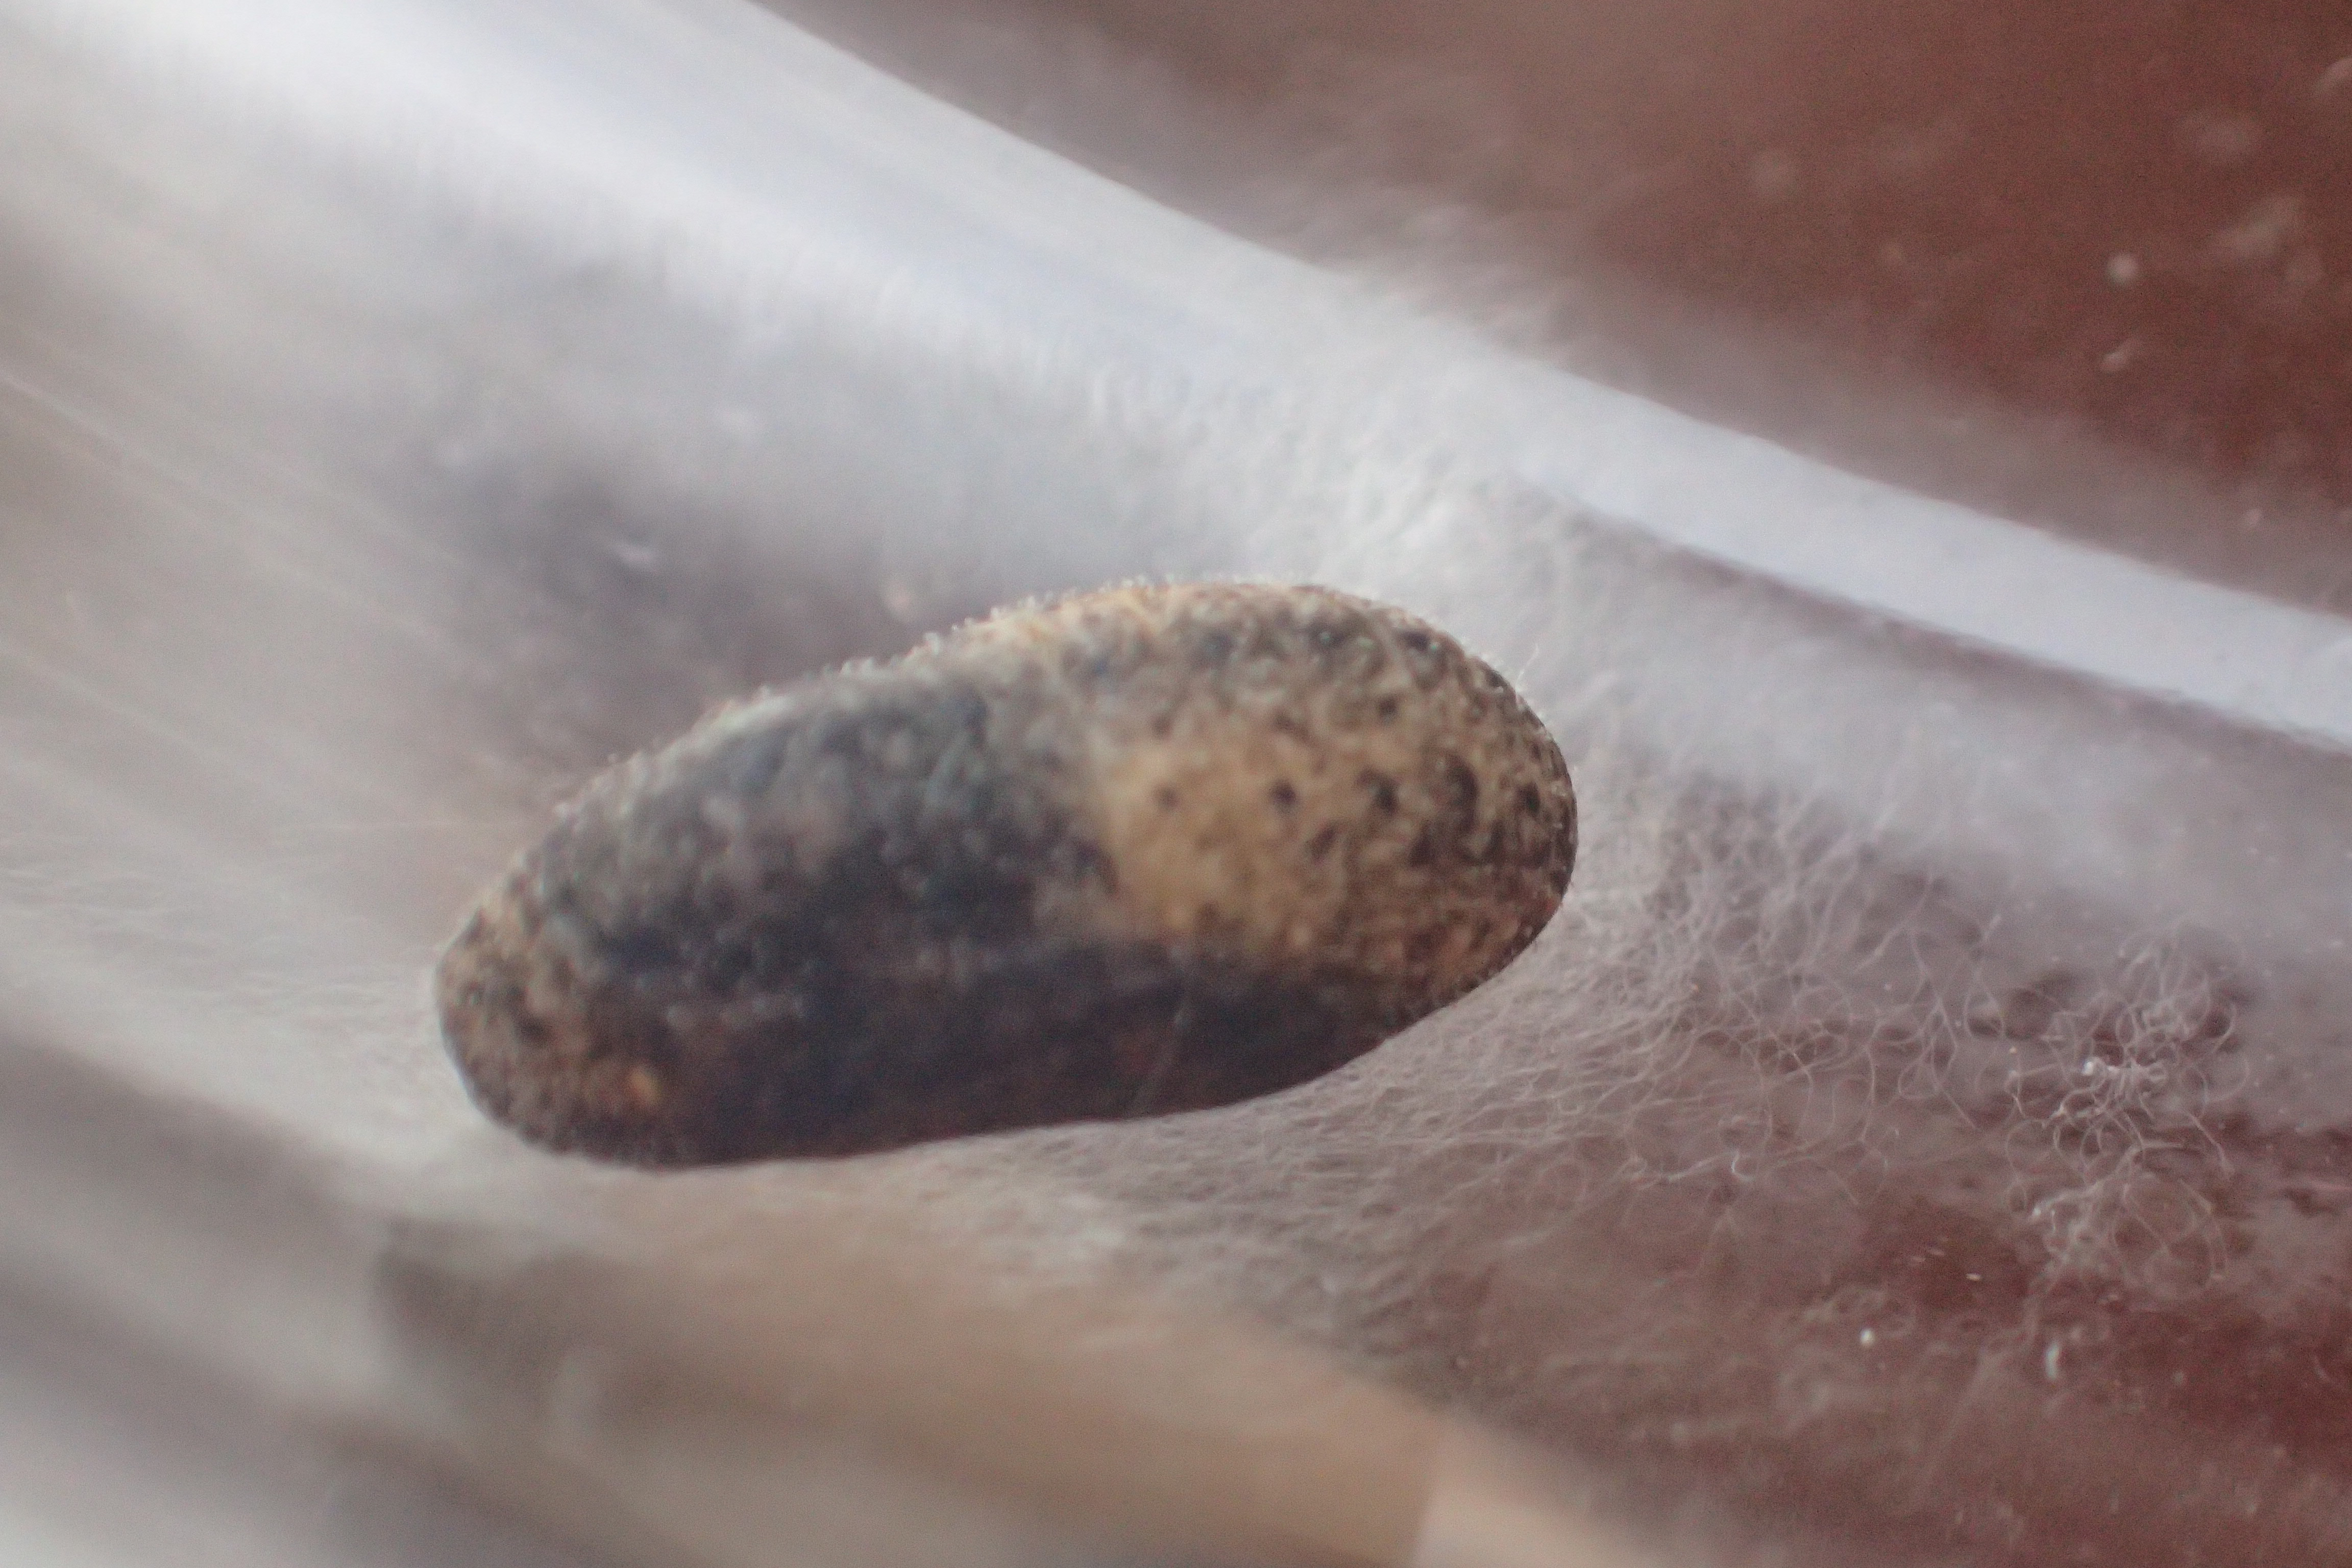
\includegraphics[width=5cm]{photo11/Larva4-pupa1.JPG}
  \end{center}
  \caption{幼虫4の蛹の色が変わってきた}
\end{figure}

\begin{figure}[htbp]
  \begin{center}
    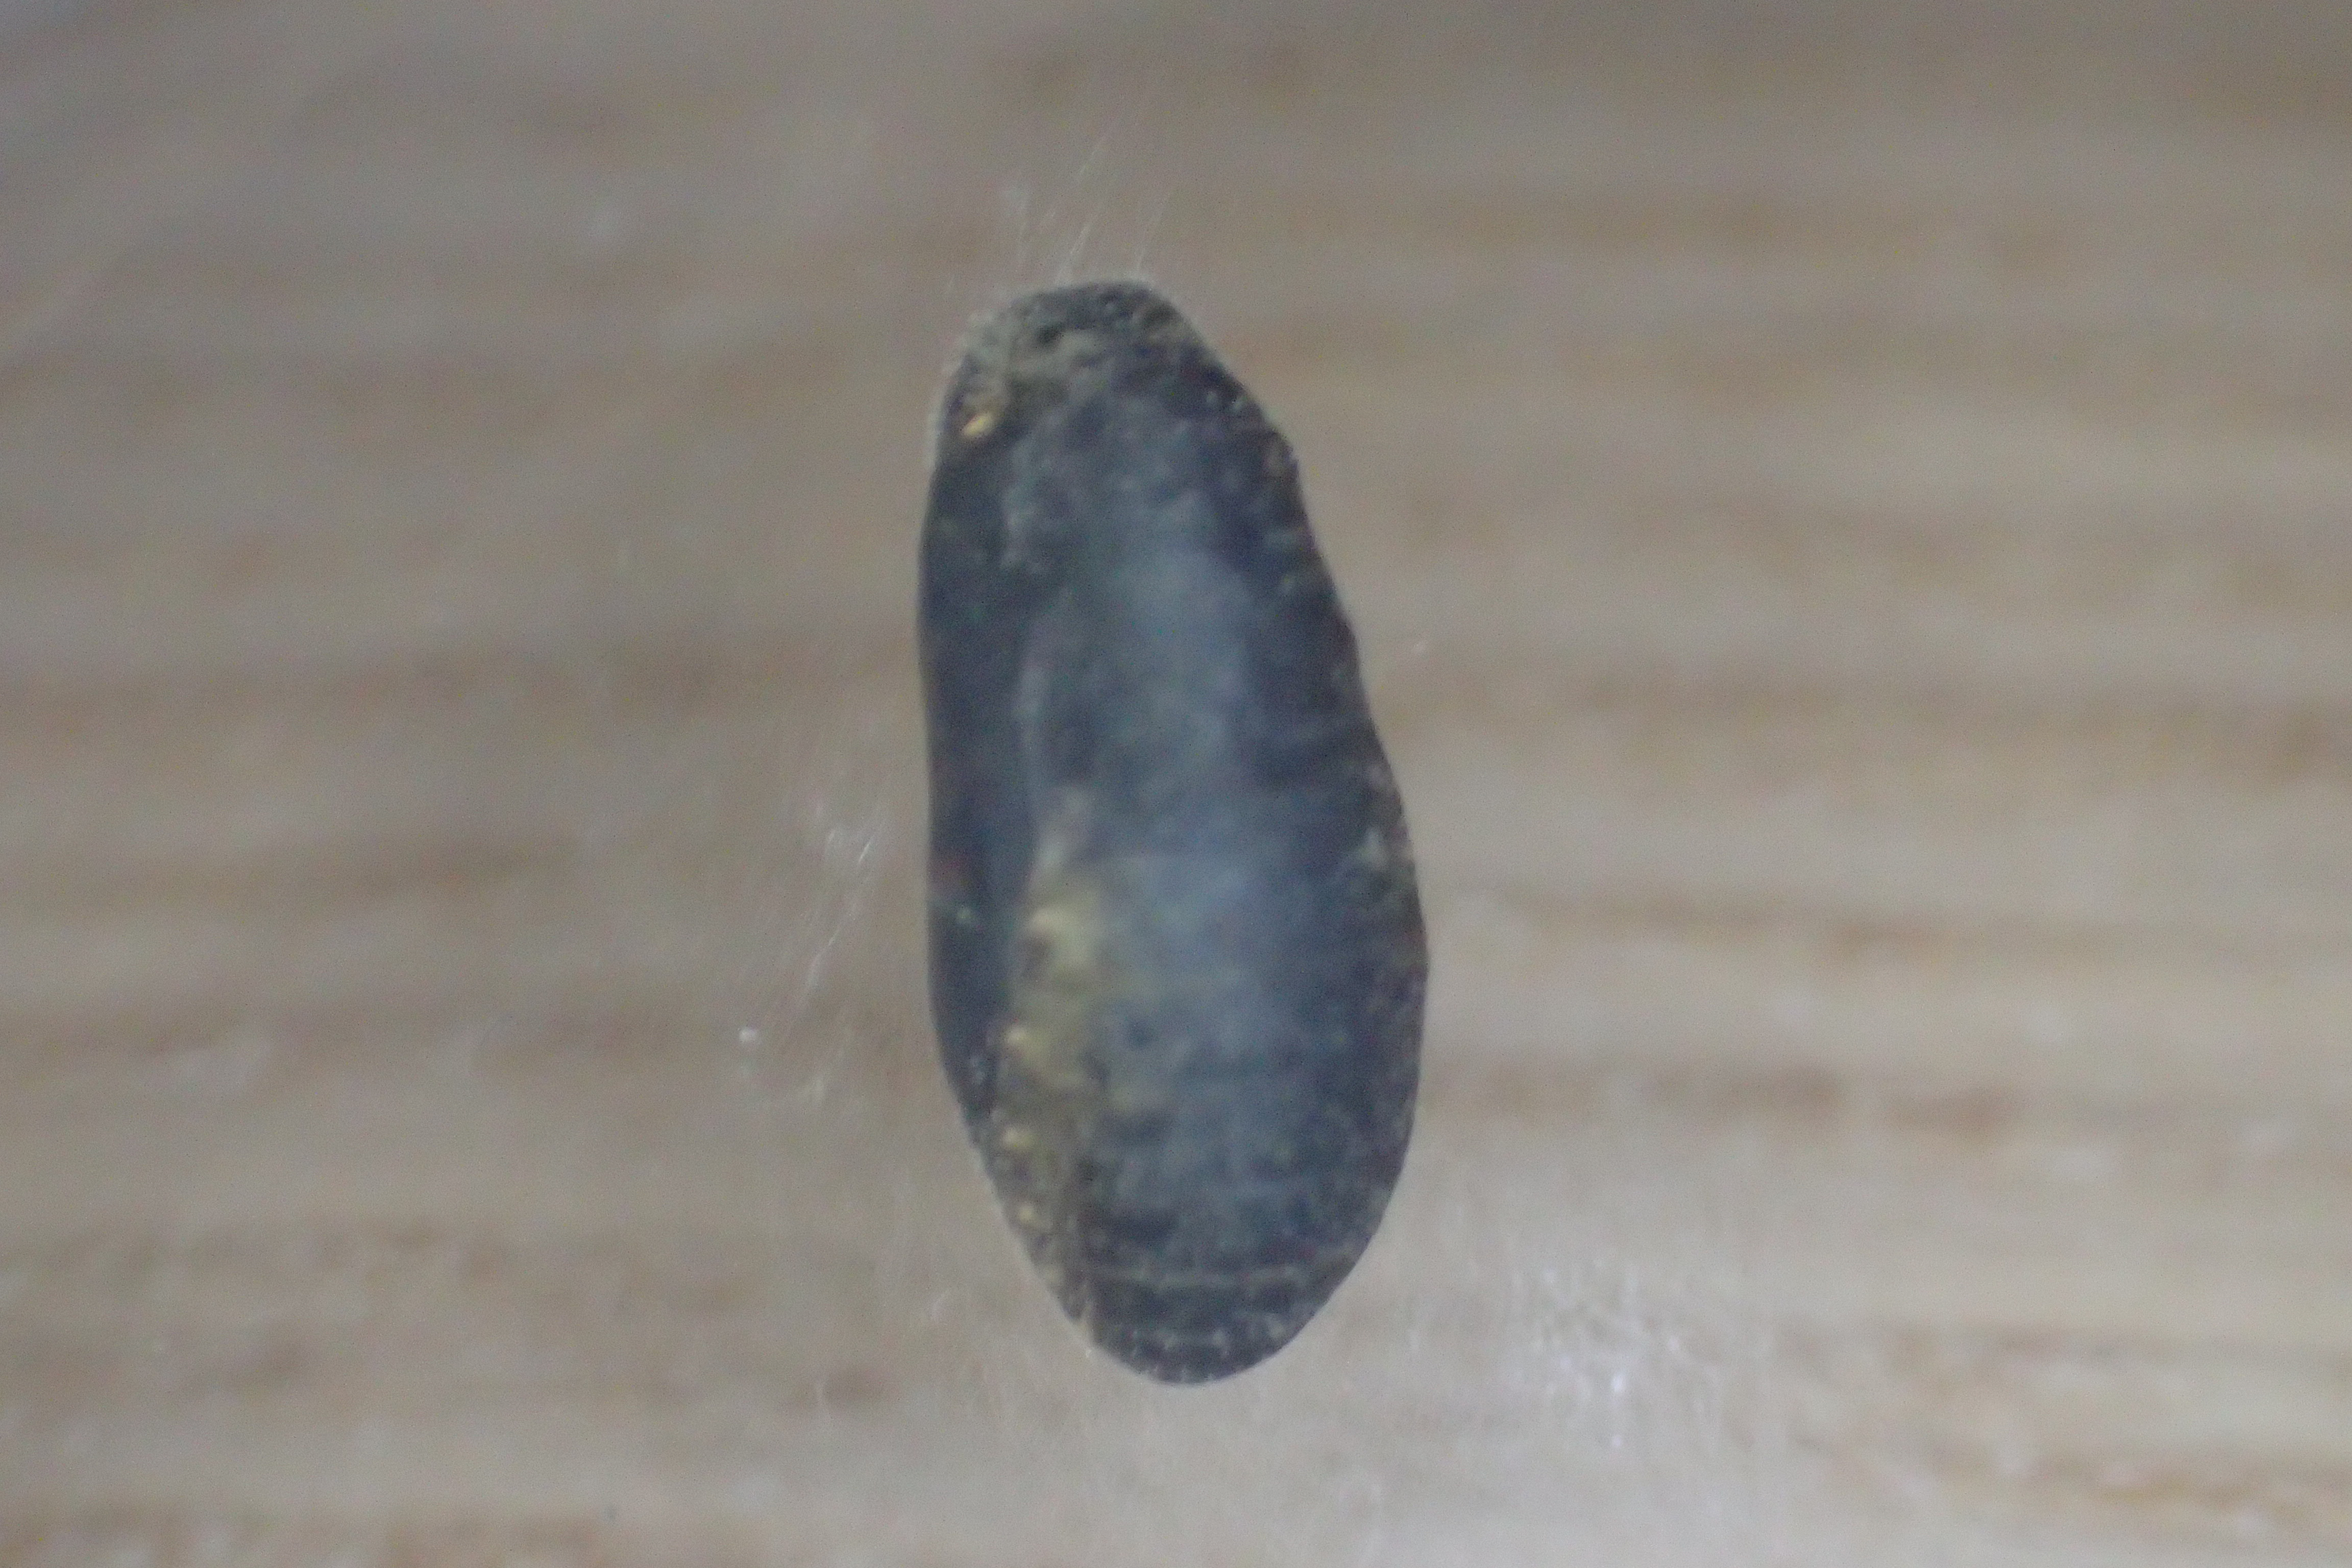
\includegraphics[width=5cm]{photo11/Larva4-pupa2.JPG}
  \end{center}
  \caption{幼虫4の蛹の色が一気に黒くなった}
\end{figure}

\begin{figure}[htbp]
  \begin{center}
    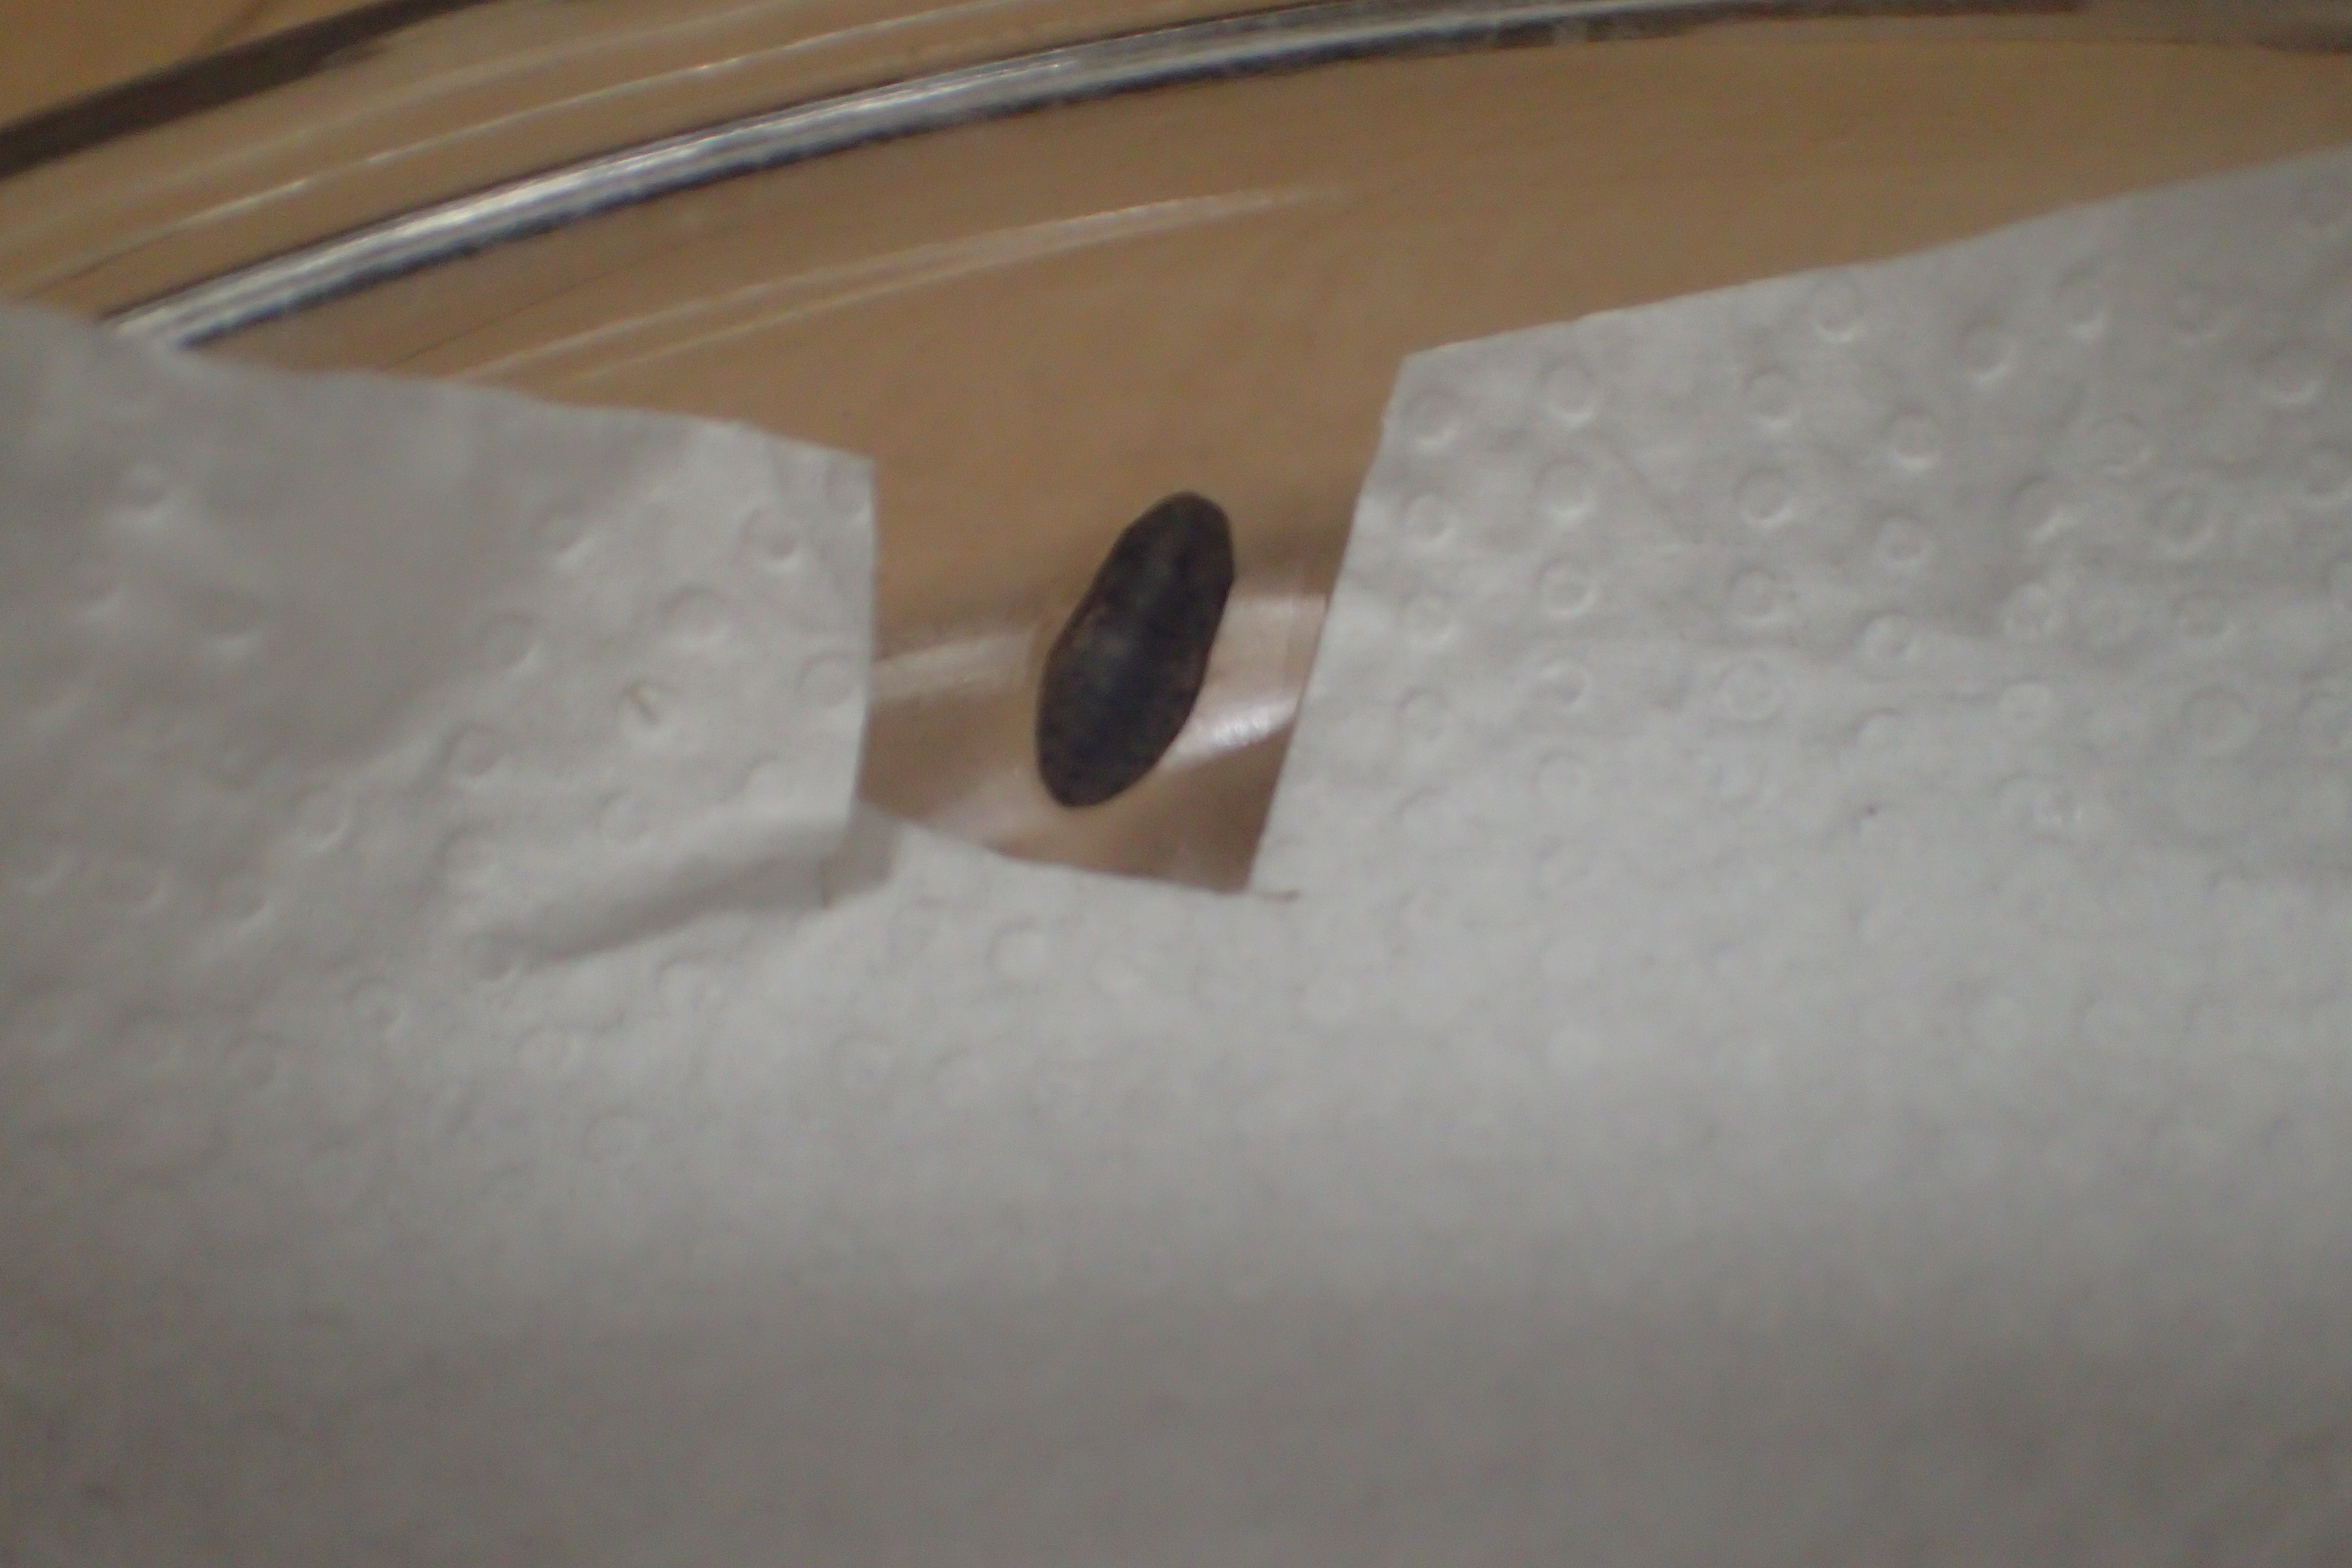
\includegraphics[width=5cm]{photo11/Larva4-pupa3.JPG}
  \end{center}
  \caption{幼虫4の羽化に備えて足場作成}
\end{figure}

\section{5/28の記録}
\subsection{10時:羽化していた}
幼虫4から羽化しており, すでに羽も伸びきっていた. 
あまり動きは活発ではないが, 飼育個体のような小ささもなく, 綺麗に羽化している. 
生殖器の形から, オスであると推測されたが, 羽をなかなか開いてくれないので鱗粉のパターンでの識別は不能. 

\begin{figure}[htbp]
  \begin{center}
    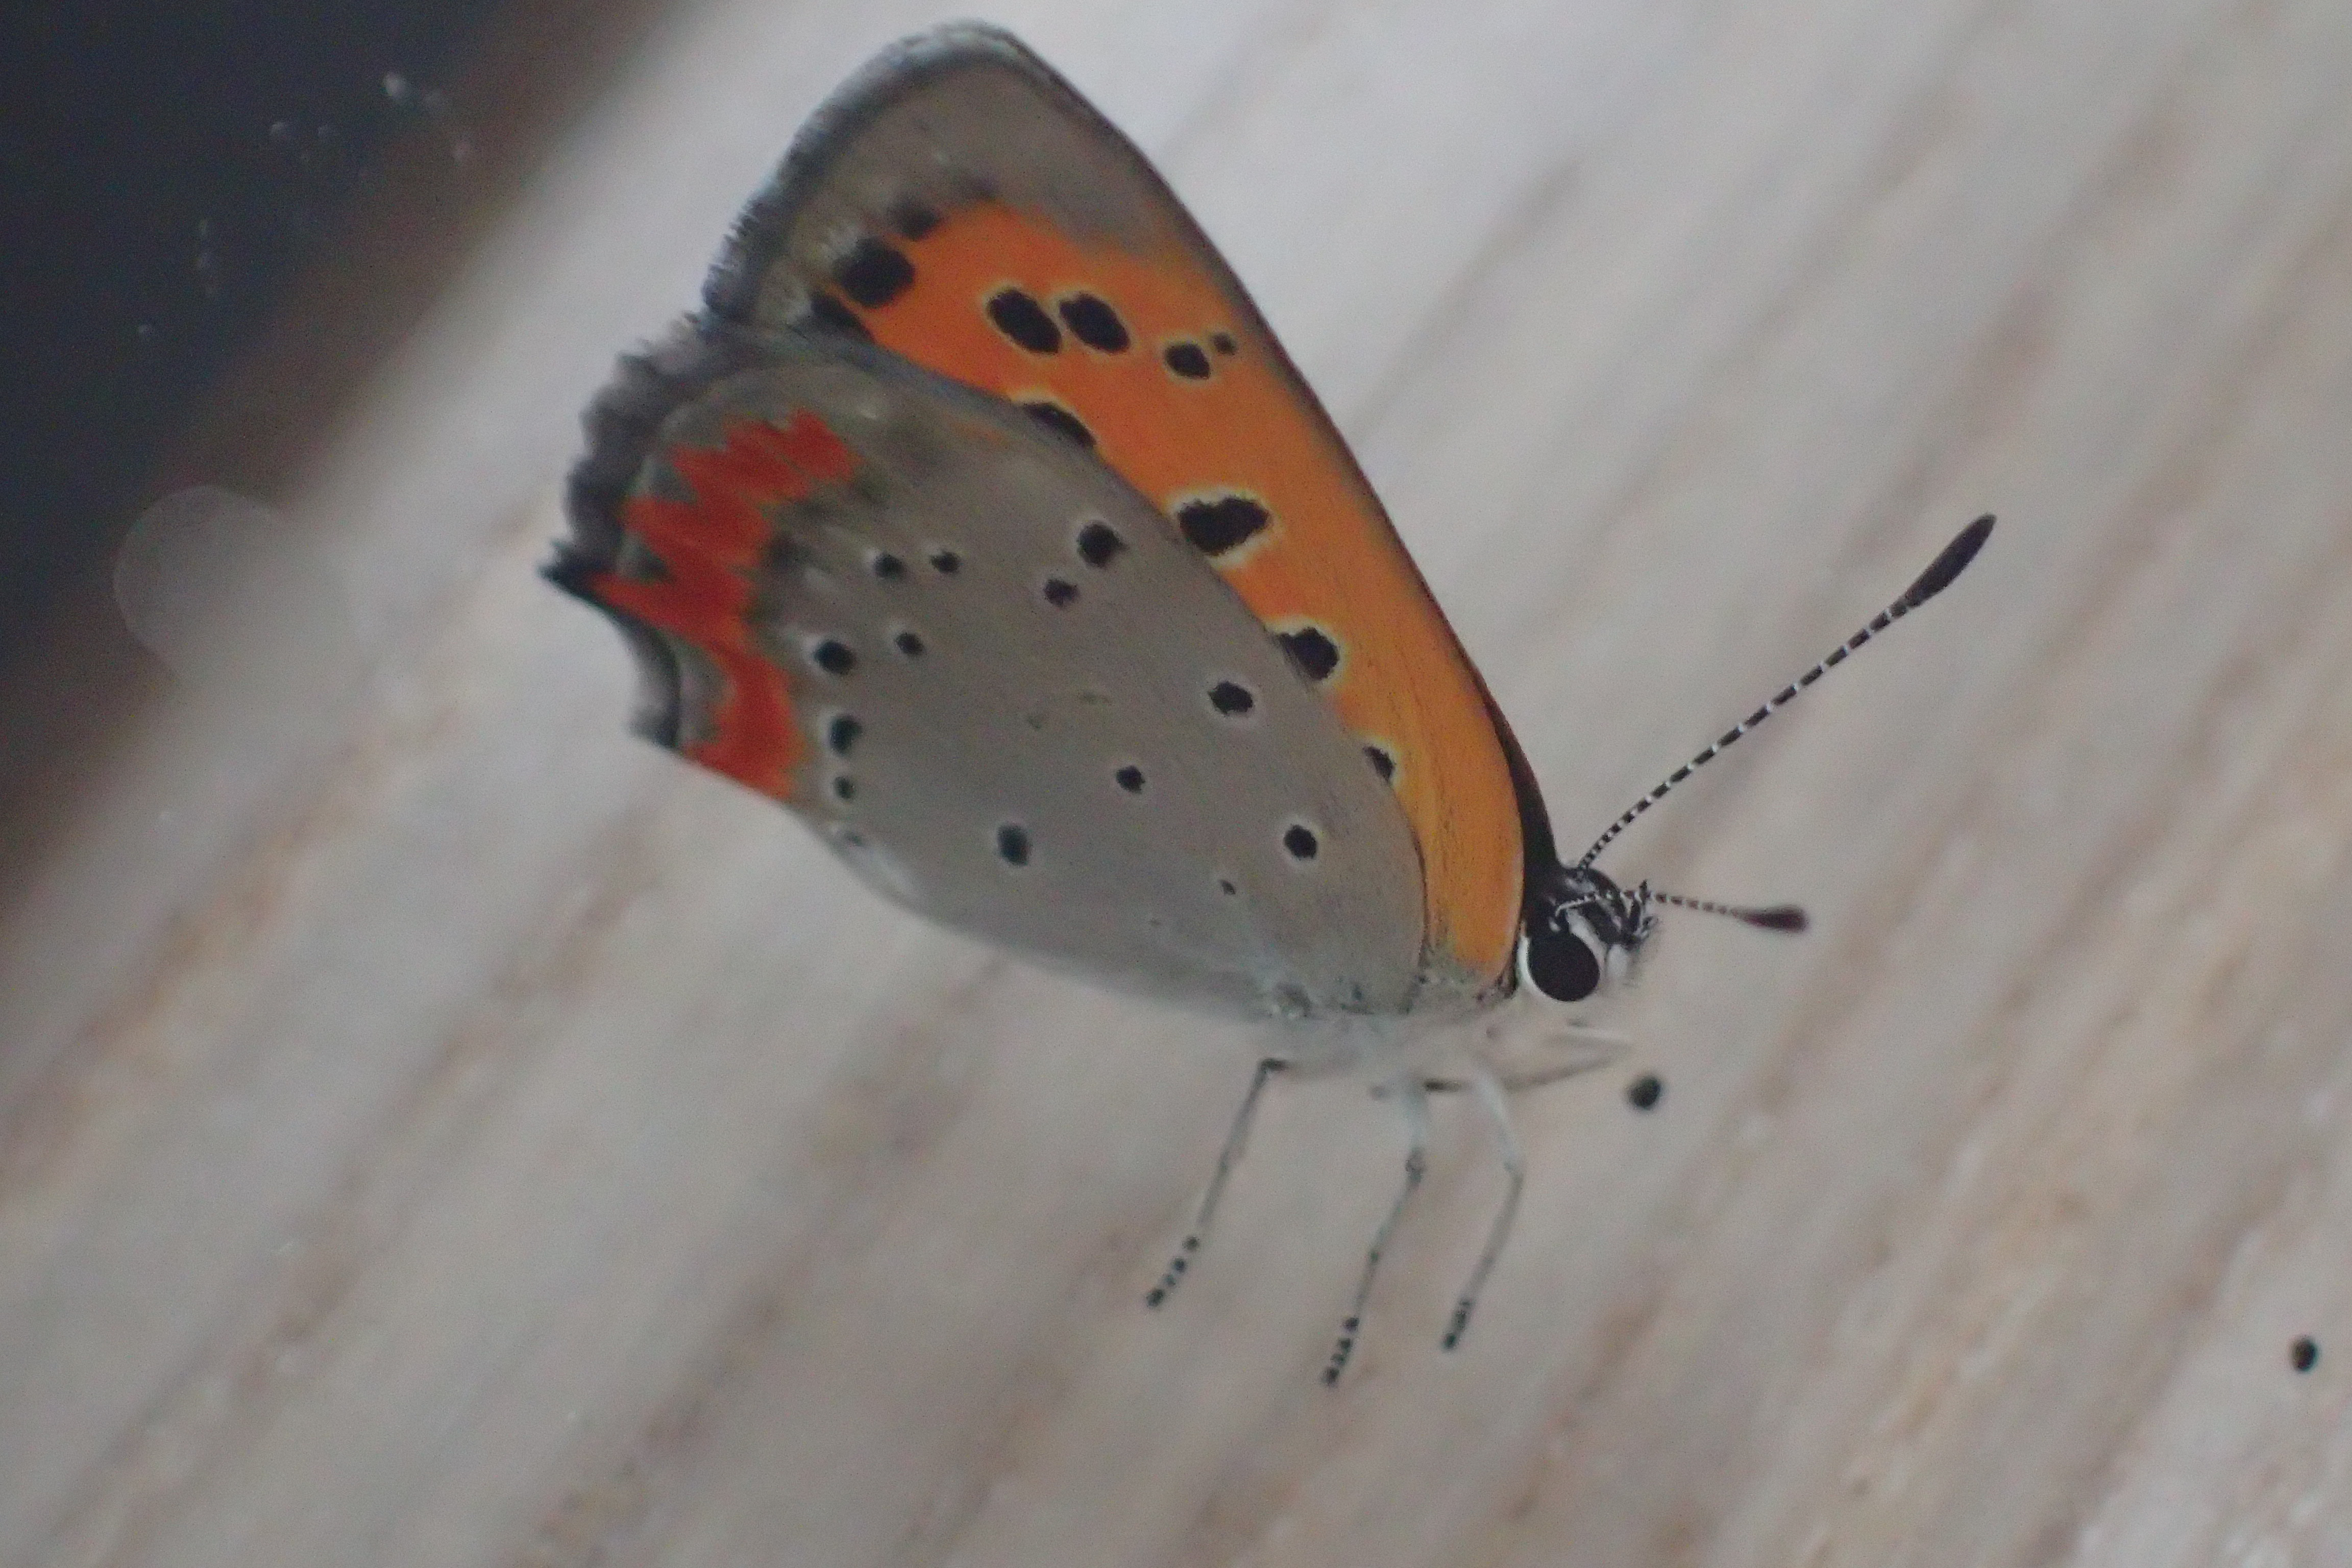
\includegraphics[width=5cm]{photo12/Larva4-emergence1.JPG}
  \end{center}
  \caption{幼虫4の羽化}
\end{figure}

\begin{figure}[htbp]
  \begin{center}
    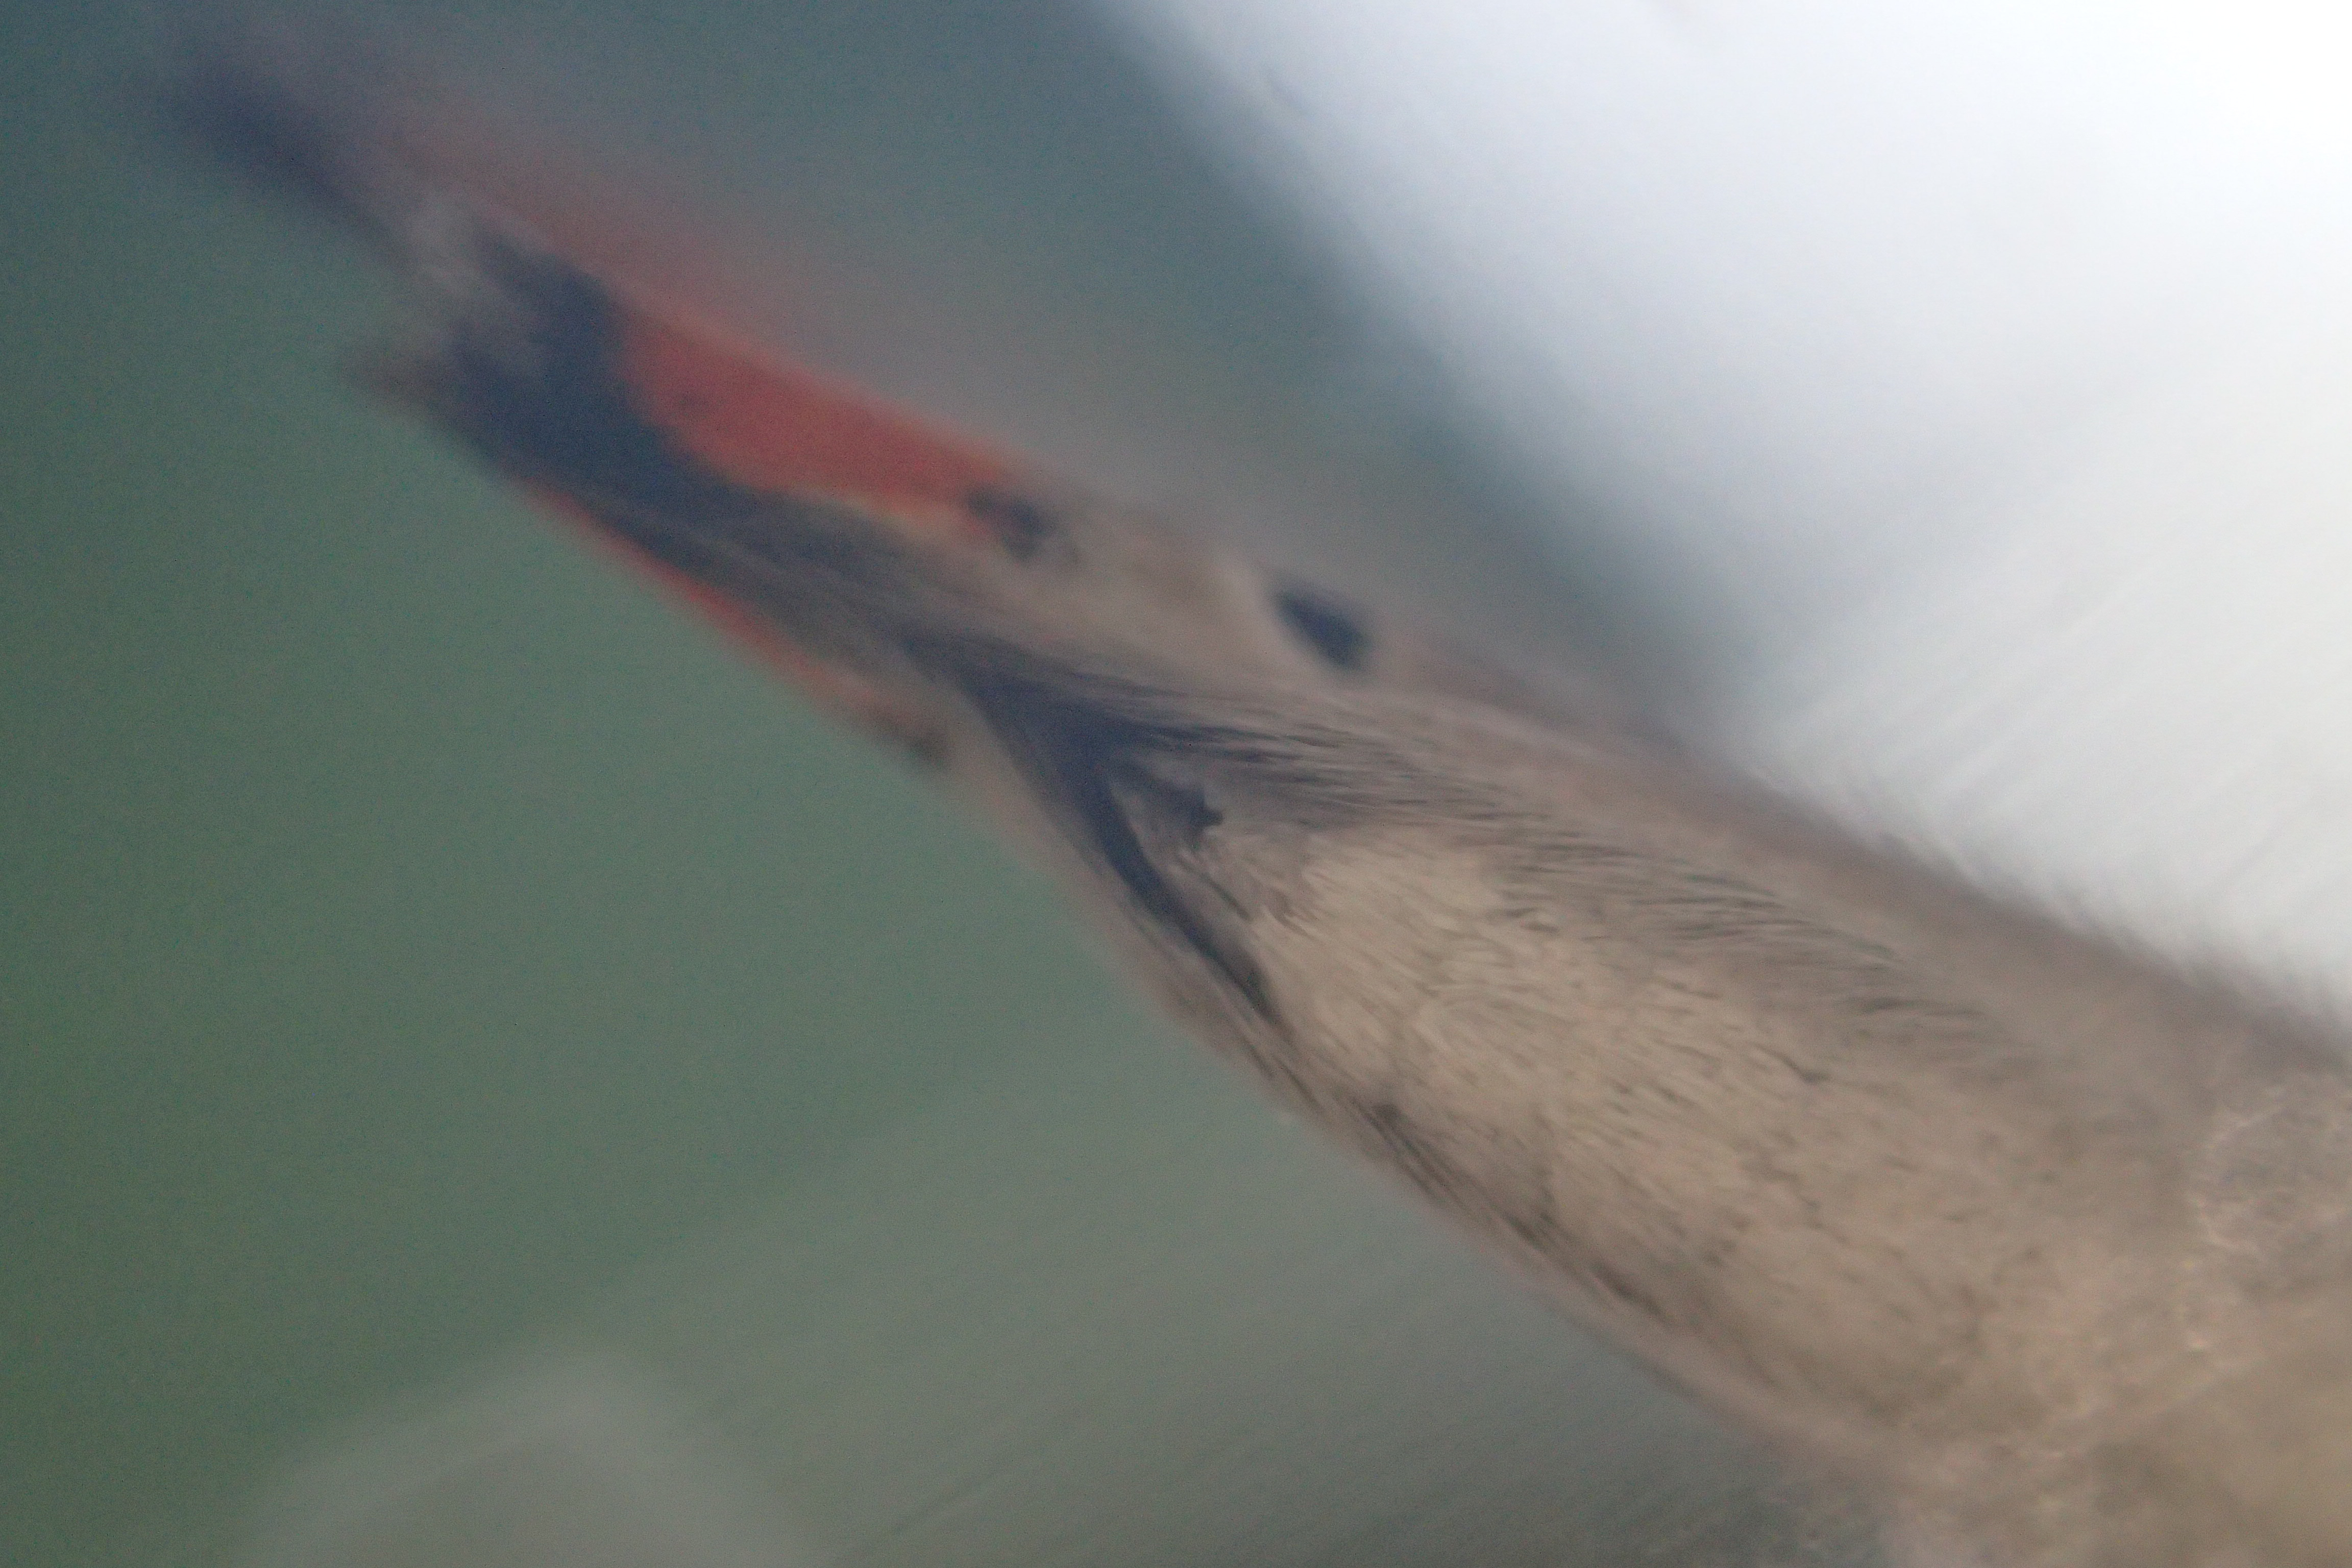
\includegraphics[width=5cm]{photo12/Larva4-abdomen.JPG}
  \end{center}
  \caption{幼虫4のは多分オス}
\end{figure}

\subsection{12時:放蝶}
いつまでも動こうとしないので, さすがに4時間も経てばOKだろうと考え, 放蝶することにした. 
途中何度か羽を開き, 典型的な夏型のオスであることが確認できた. 

\begin{figure}[htbp]
  \begin{center}
    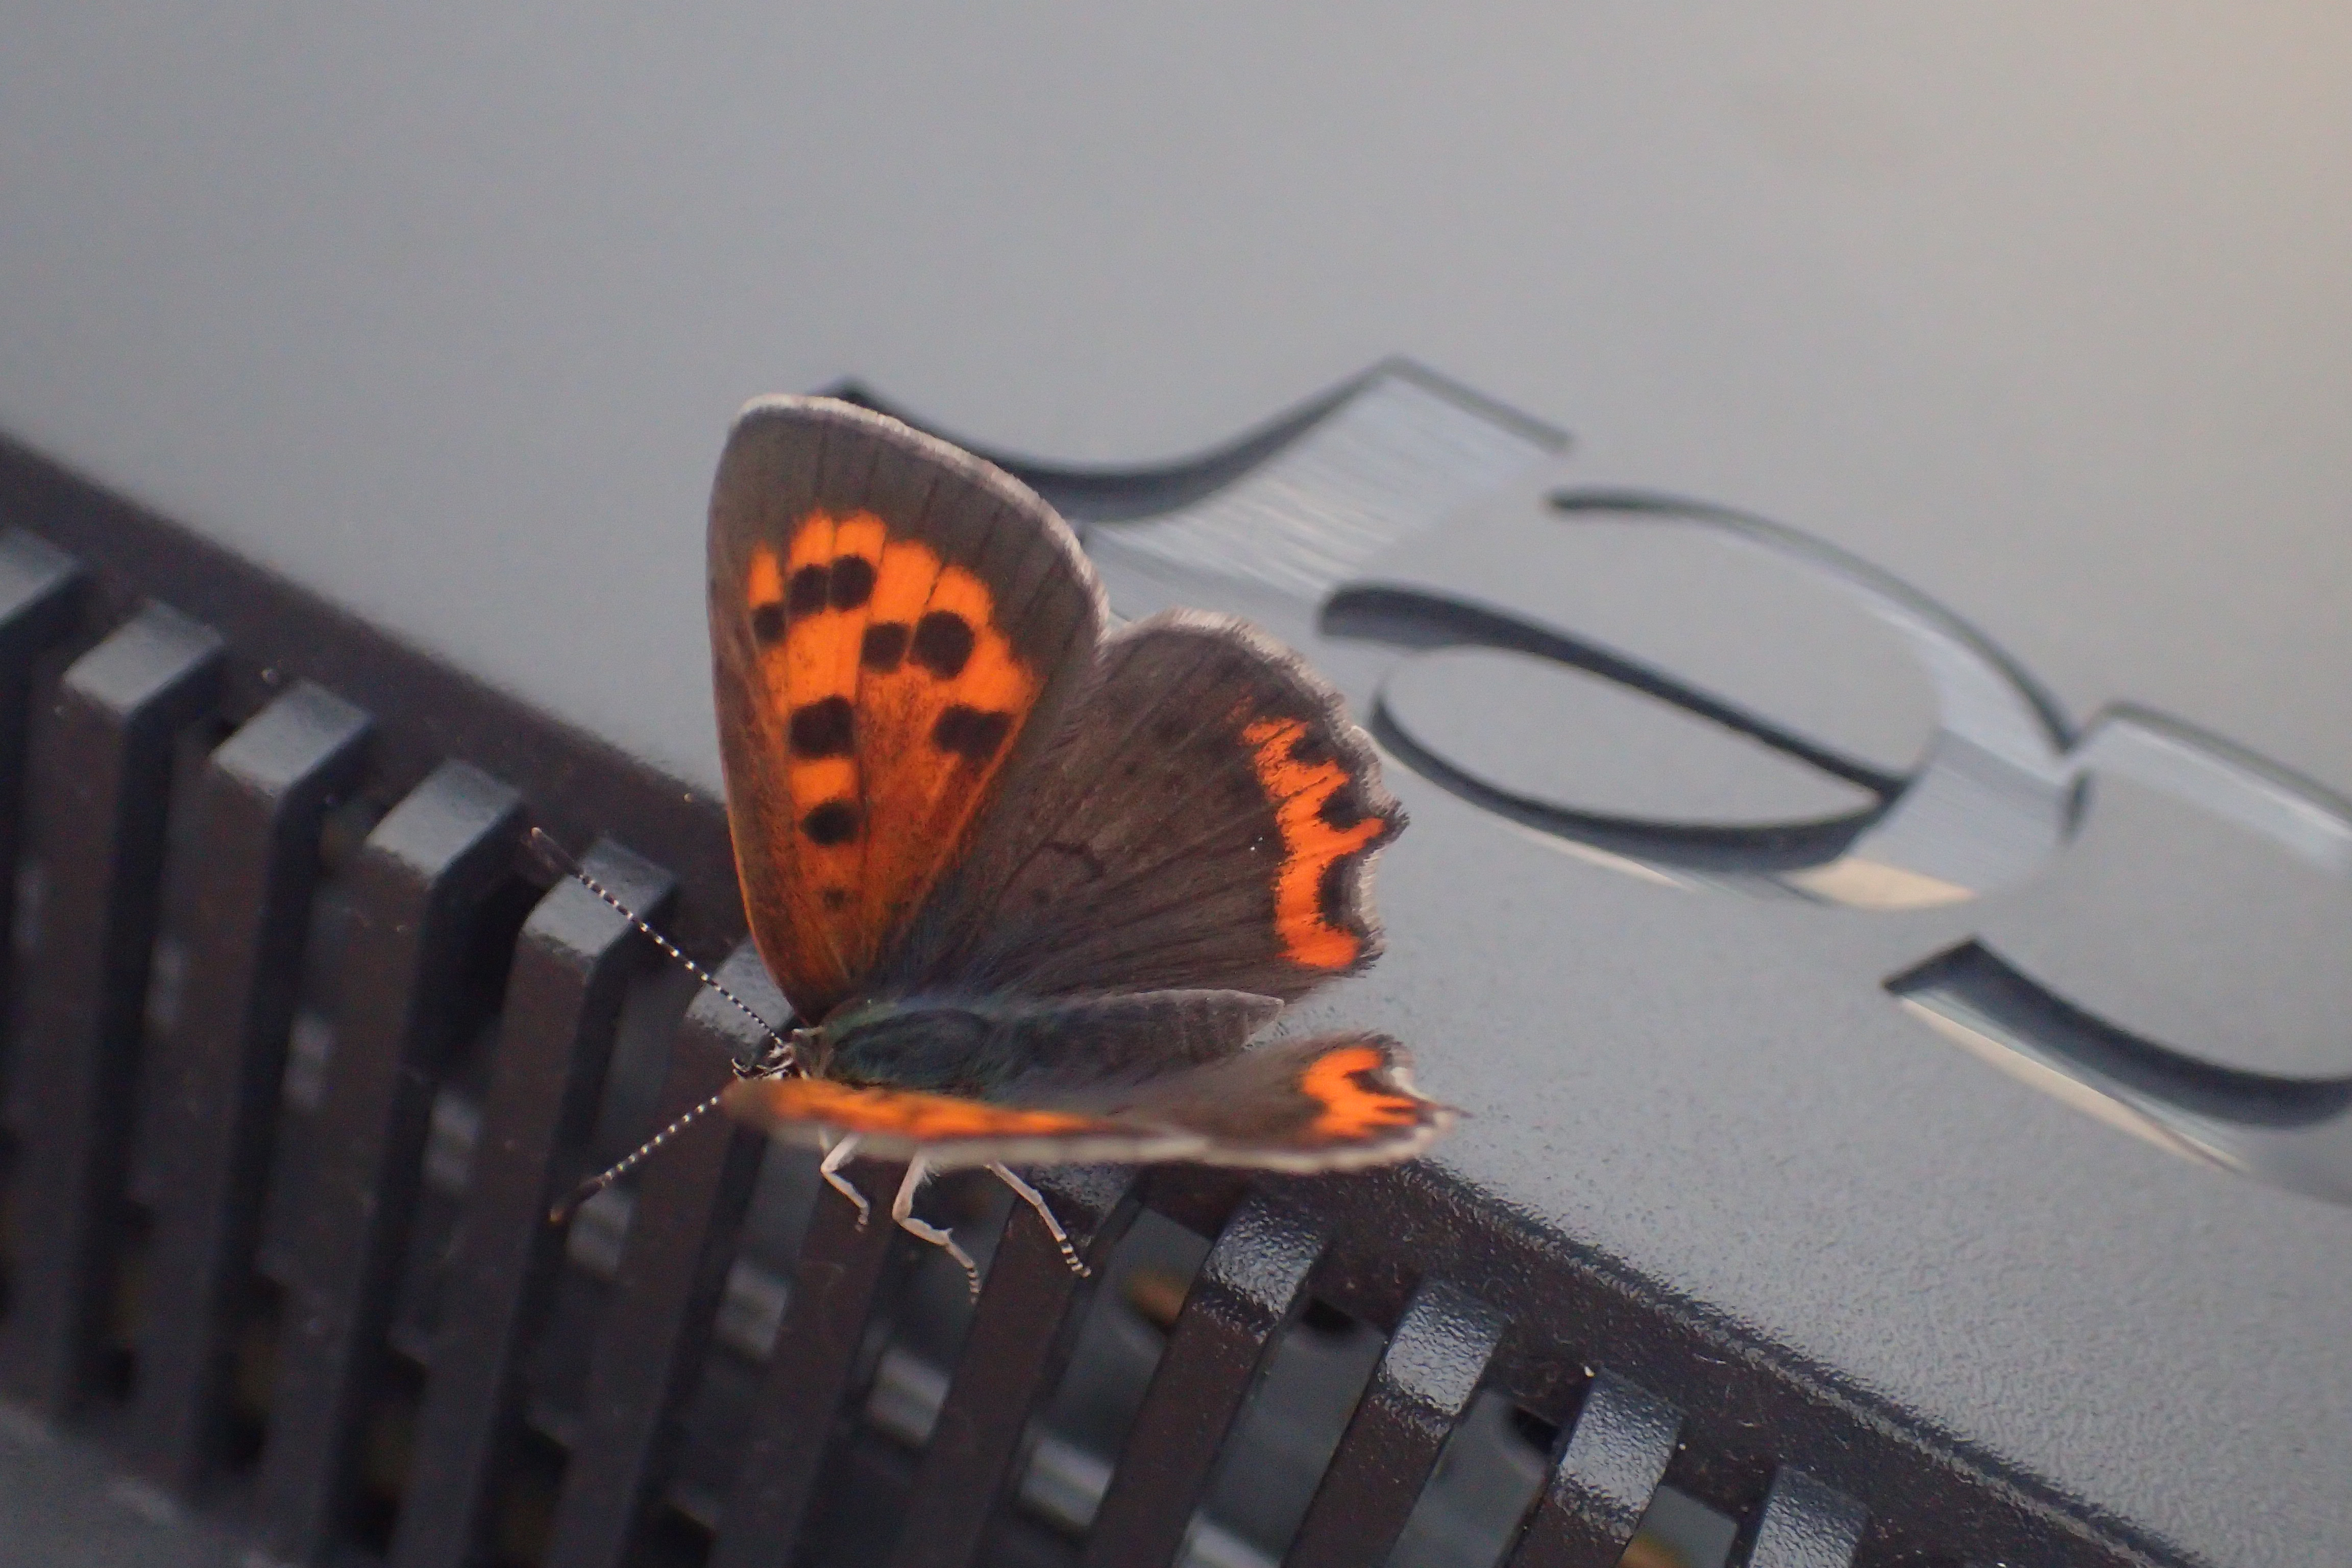
\includegraphics[width=5cm]{photo12/Larva4-fly.JPG}
  \end{center}
  \caption{幼虫4やっと羽を開いた}
\end{figure}

\section{5/29の記録}
\subsection{22時:蛹に羽の輪郭が見えている}
蛹を見ると, 蝶の羽の輪郭らしき筋が見える. 

\begin{figure}[htbp]
  \begin{center}
    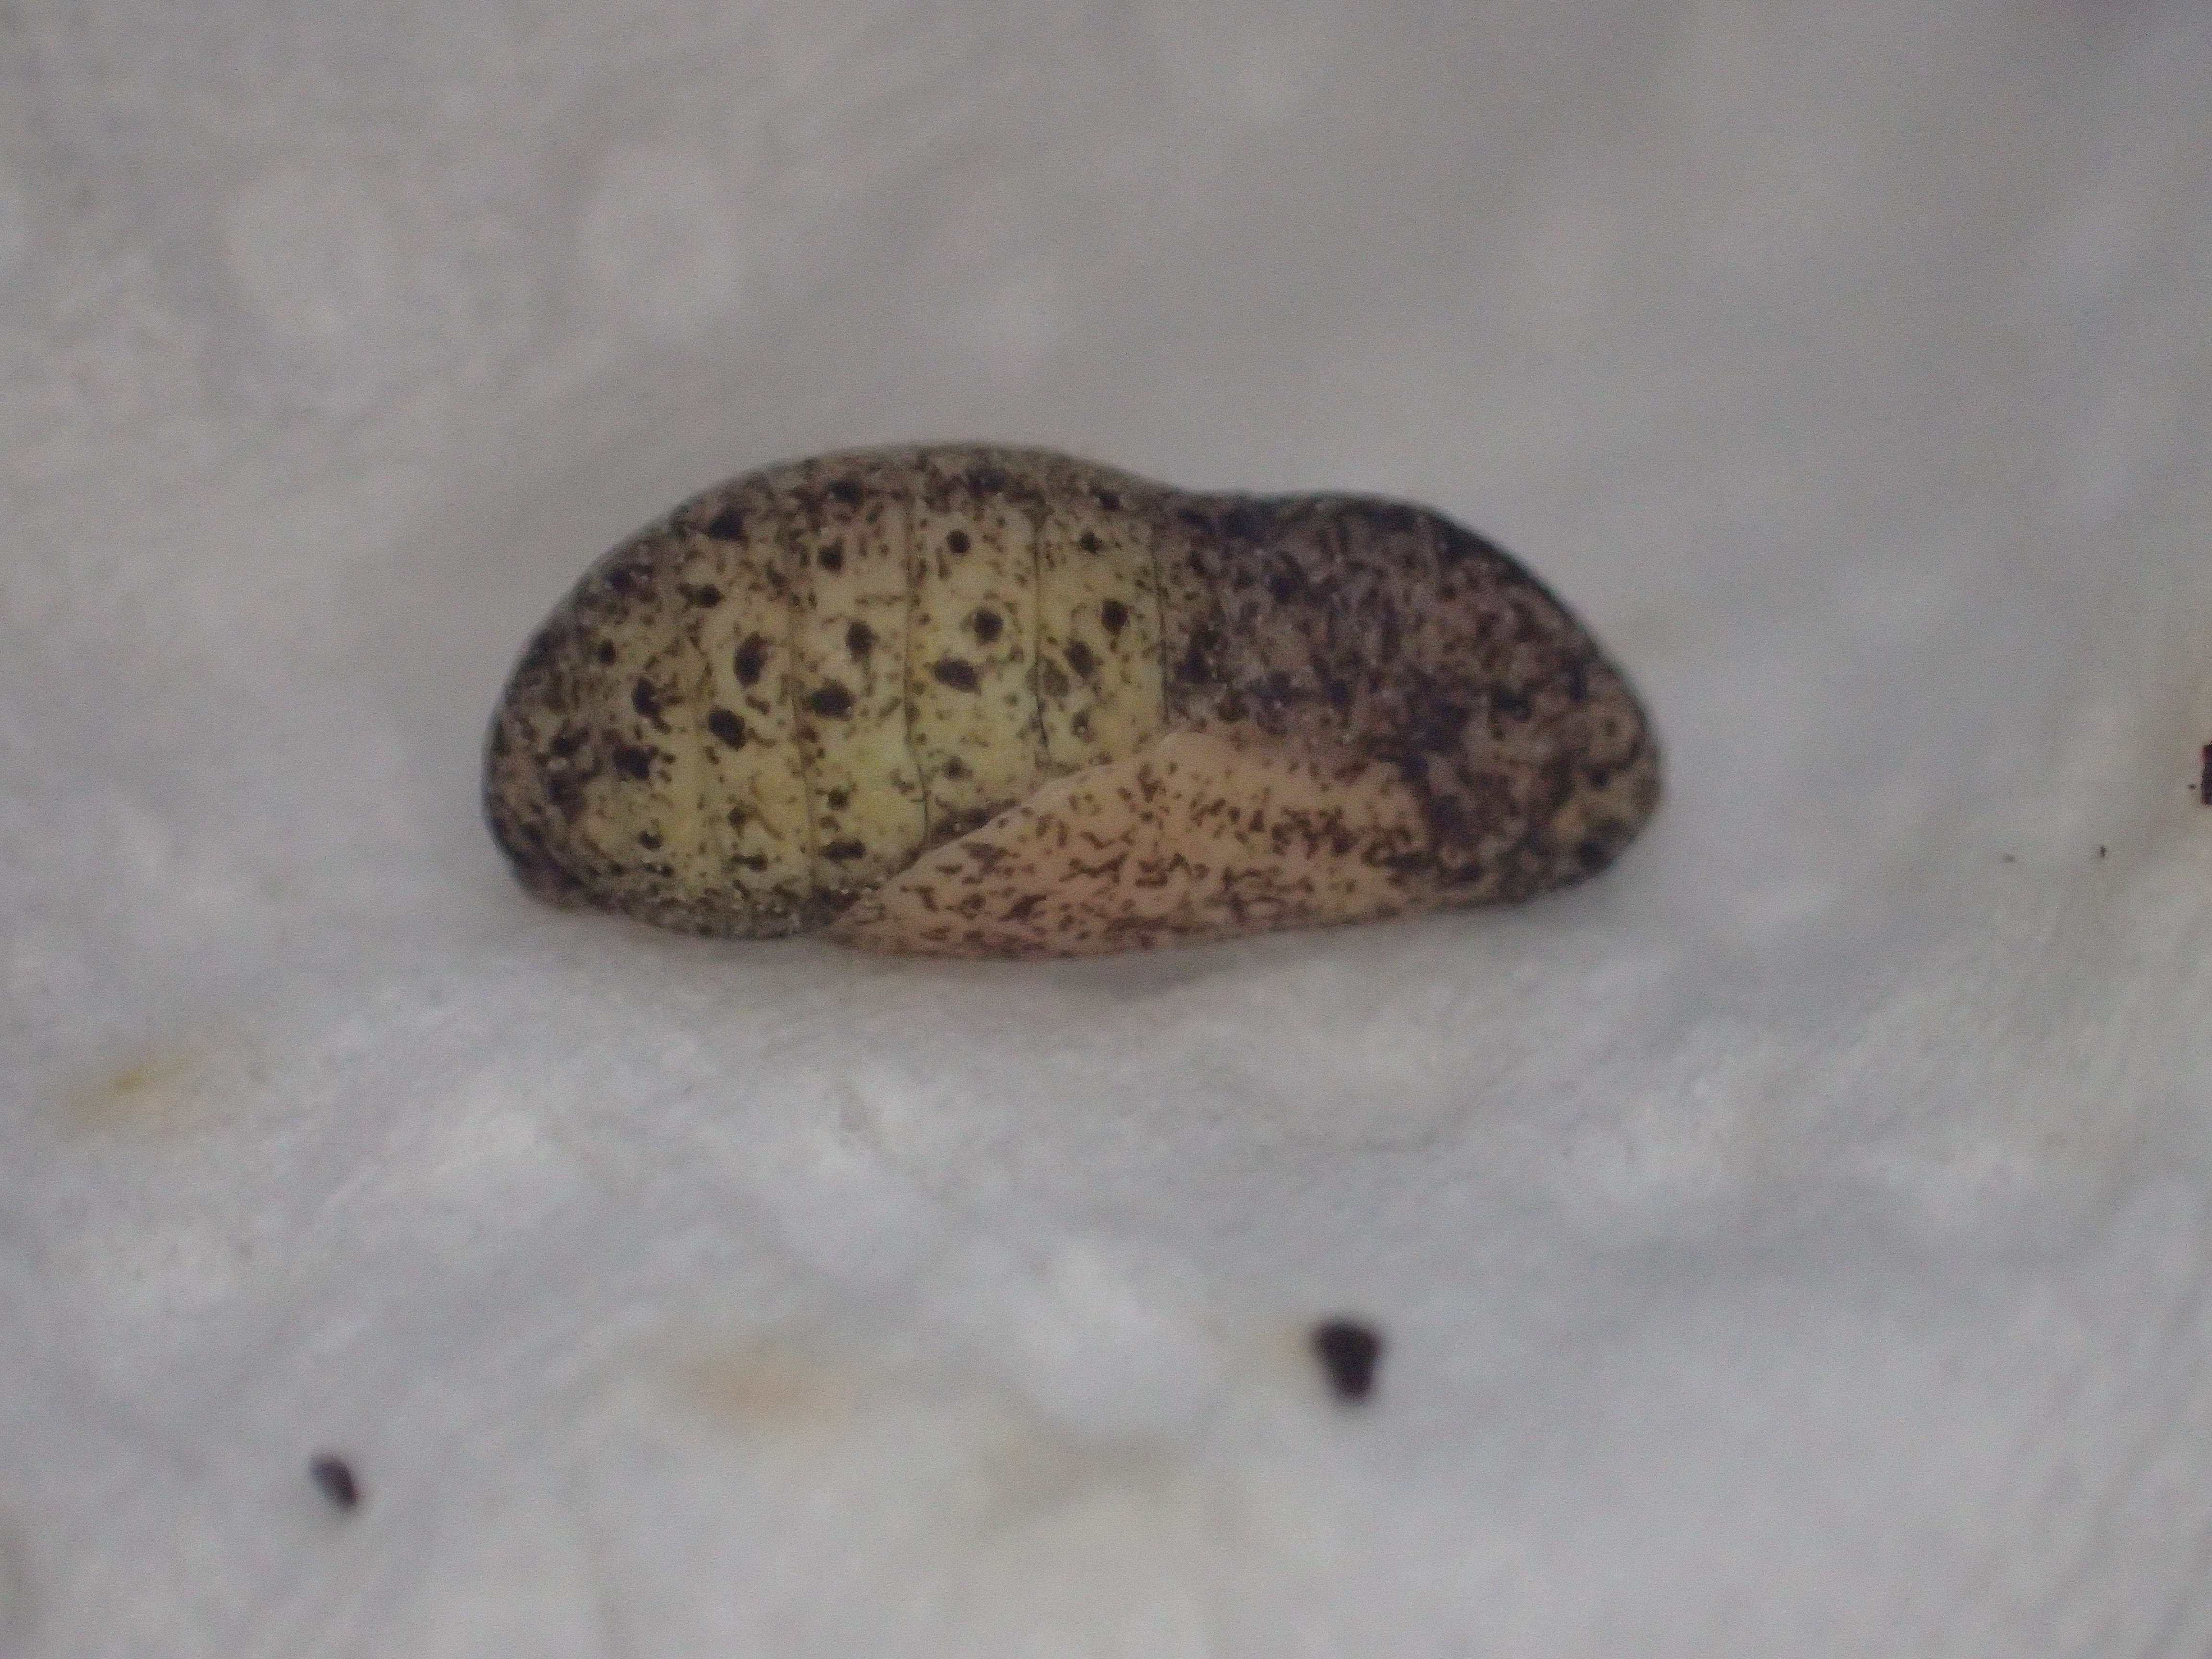
\includegraphics[width=5cm]{photo13/Larva5-pupa.JPG}
  \end{center}
  \caption{幼虫5蛹に蝶の羽の筋が見える}
\end{figure}

\section{5/31の記録}
\subsection{18時:幼虫5の蛹が黒くなってきた}
幼虫4のときと同様に, ある日突然色が変化しだす. 

\begin{figure}[htbp]
  \begin{center}
    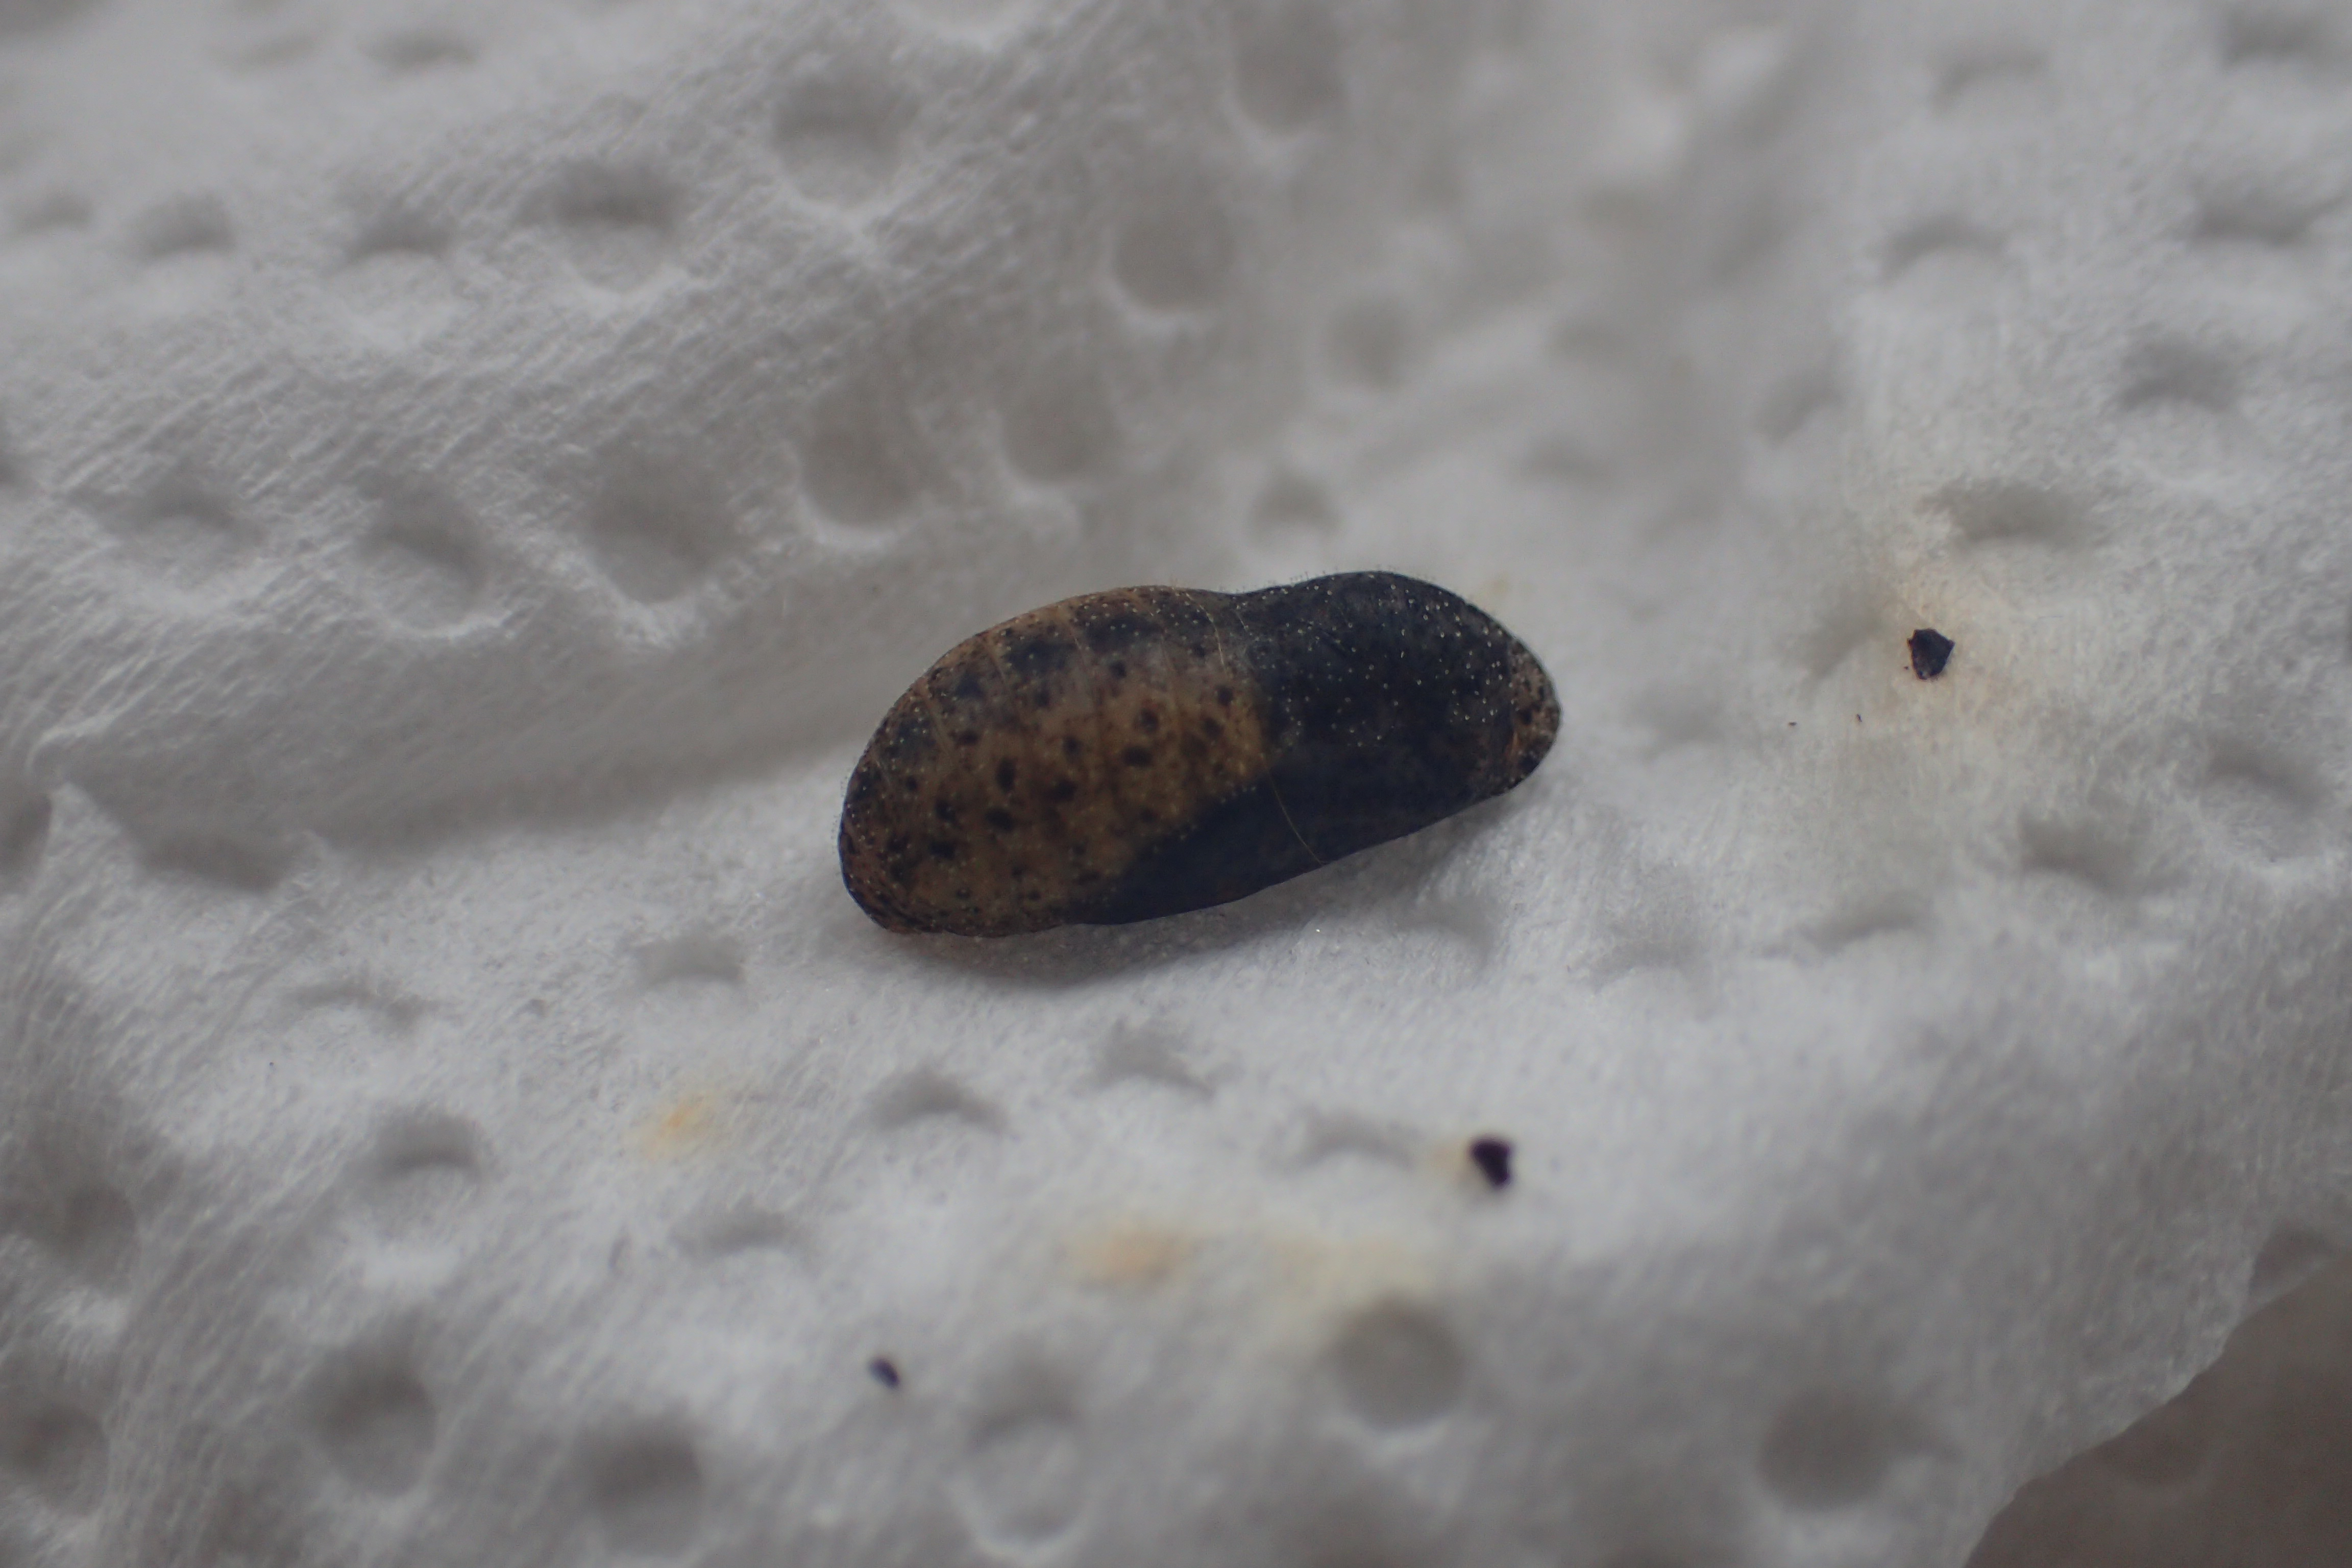
\includegraphics[width=5cm]{photo14/Larva5-pupa.JPG}
  \end{center}
  \caption{幼虫5蛹の色が変化しだす}
\end{figure}

\subsection{21時:急激に色が変化した}
幼虫4のときと同様に, 数時間の間に一気に真っ黒に変化した. 
また, 今回も寝ている間に羽化するパターンだろう. 

\begin{figure}[htbp]
  \begin{center}
    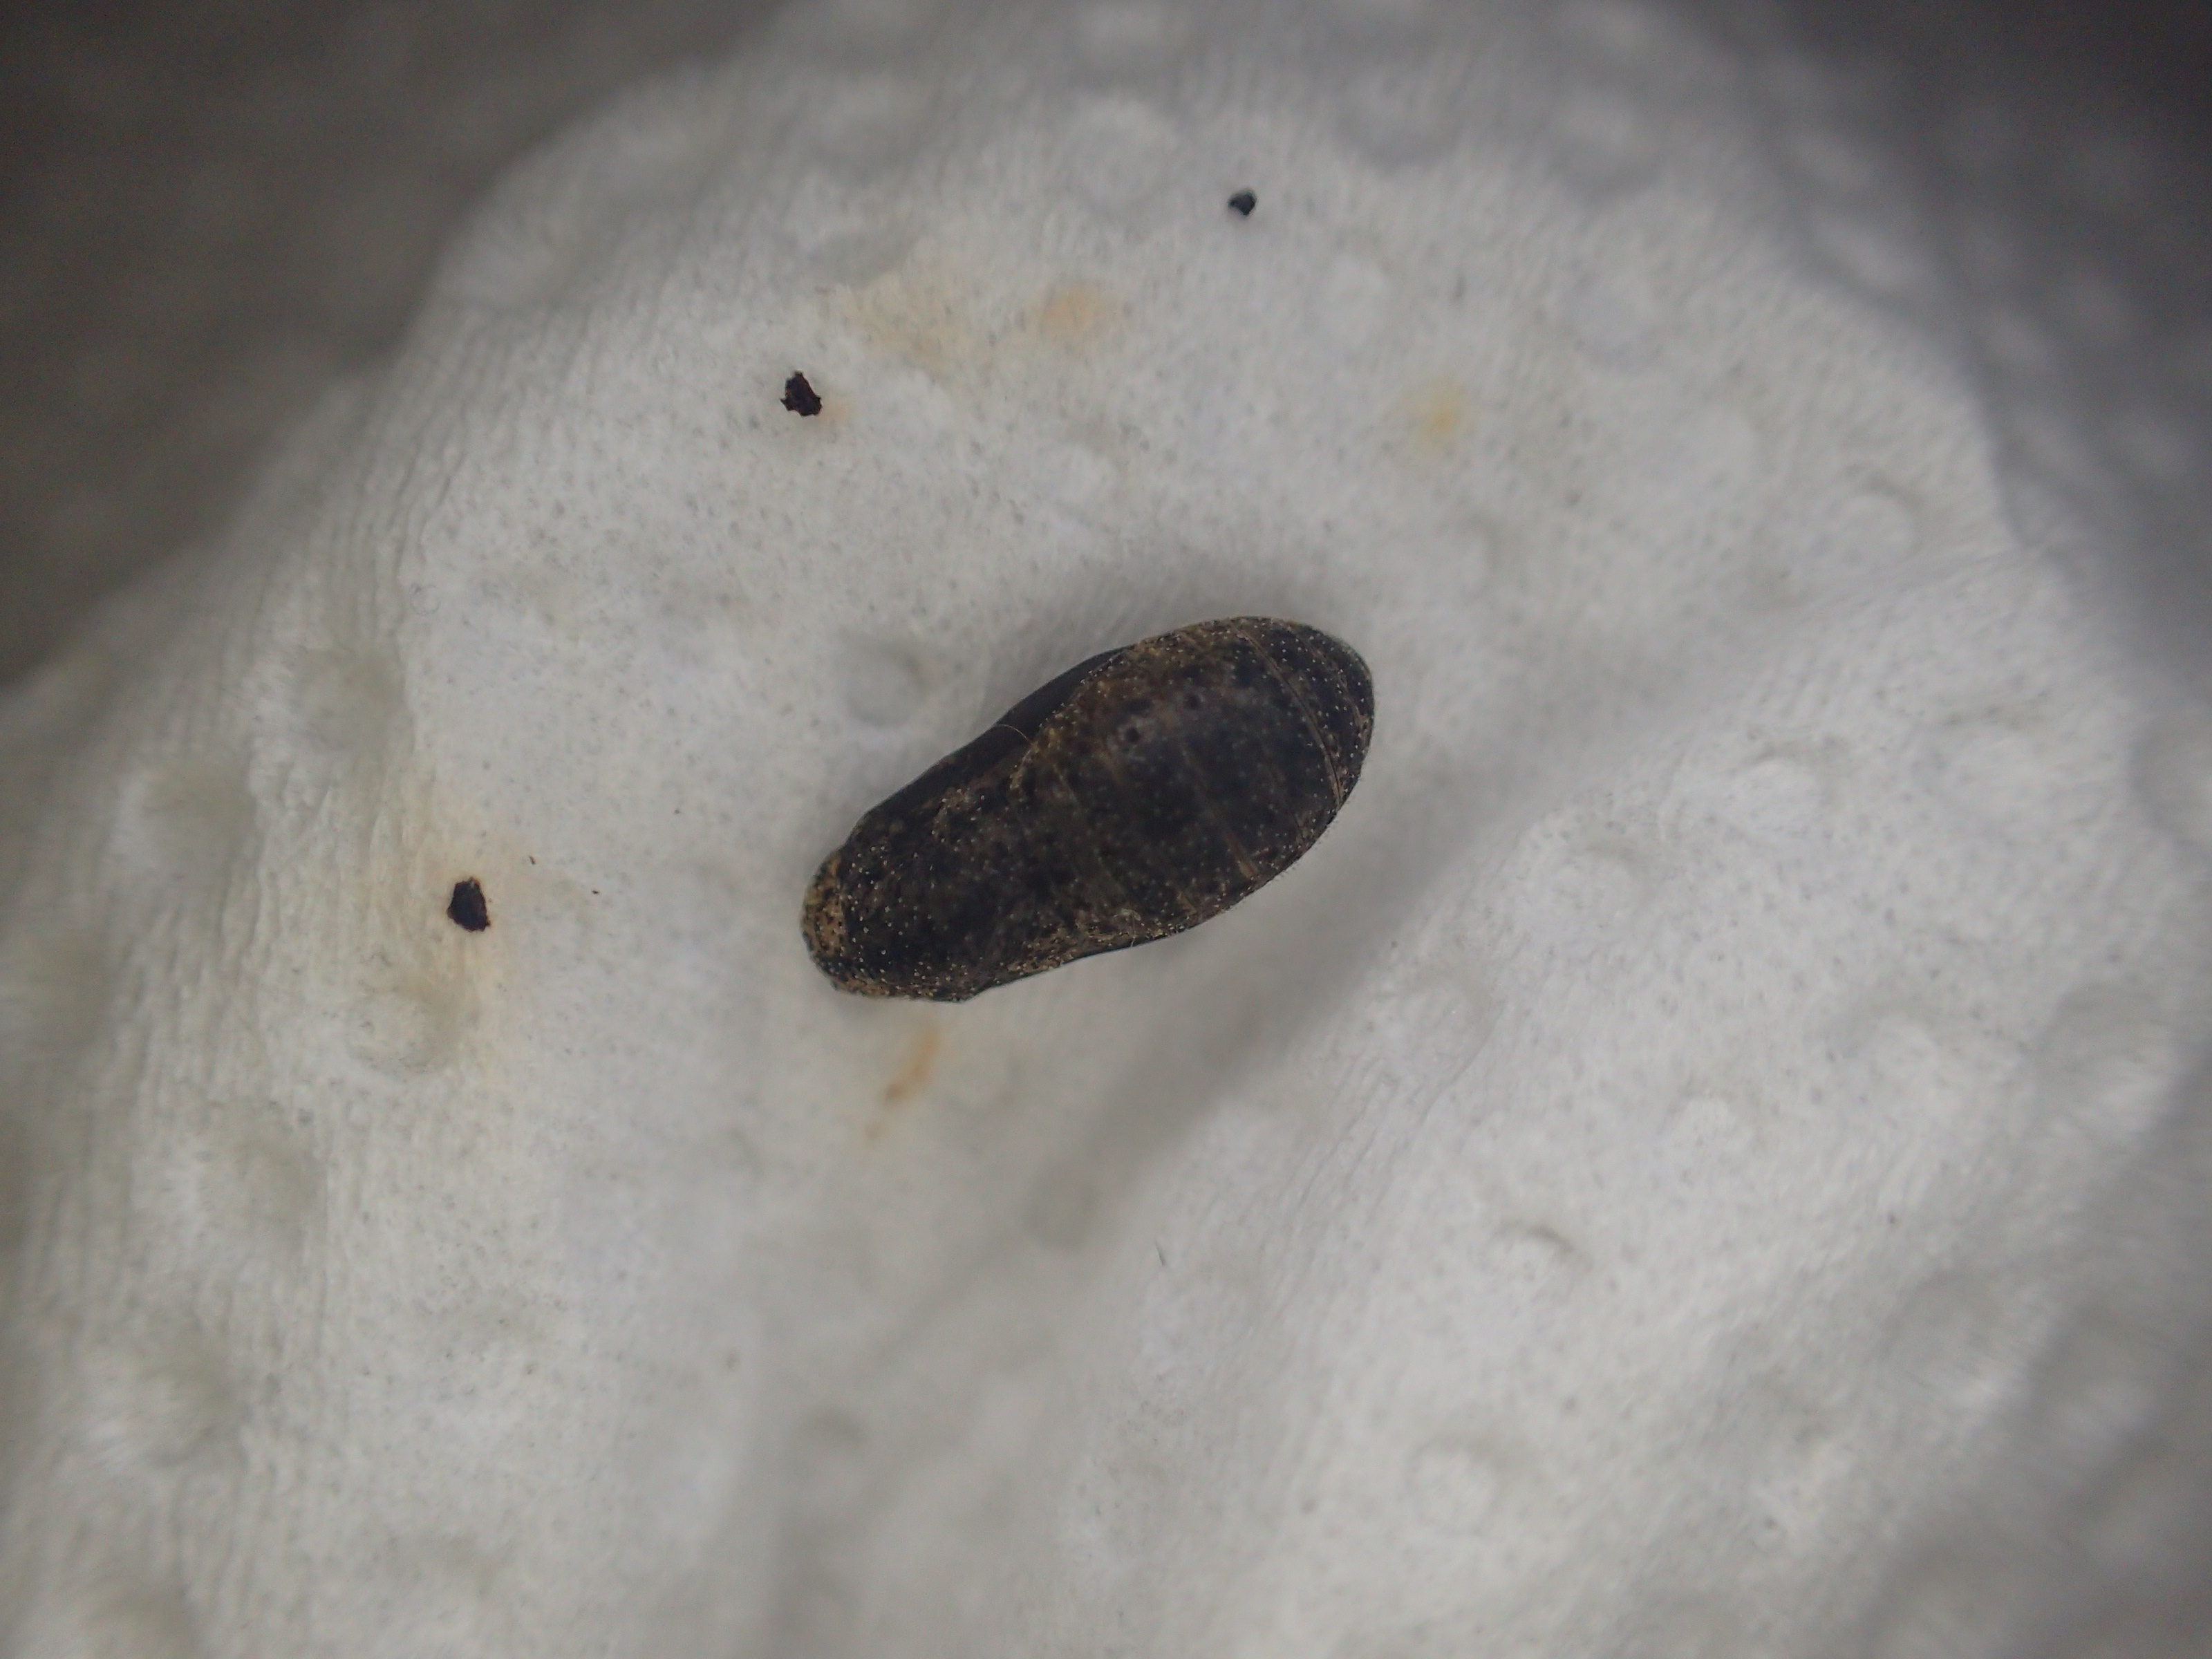
\includegraphics[width=5cm]{photo14/Larva5-pupa2.JPG}
  \end{center}
  \caption{幼虫5蛹の色が急激に変化}
\end{figure}

\end{document}
